\documentclass[11pt]{book}
\usepackage[]{authblk}
\usepackage{graphicx}
\usepackage{tabularx}
%\usepackage{color}
\usepackage{colortbl}
\usepackage[usenames,dvipsnames,table]{xcolor}
\usepackage{booktabs}
\usepackage{longtable}
\usepackage{hanging}
\usepackage{indentfirst}
\usepackage{setspace}
\usepackage{enumitem}
\usepackage{verbatim}
\usepackage{upgreek}
\usepackage{framed}
\usepackage{ textcomp }
\usepackage{url}
\usepackage{soul}
\usepackage{amsmath, amsfonts,amssymb,mathrsfs}
\usepackage{fancyhdr}
\usepackage[compact]{titlesec}
\usepackage[T1]{fontenc}
\usepackage{lmodern}
\usepackage{float}
\usepackage[caption = false]{subfig}
\usepackage{fancybox}
\usepackage{fixltx2e}

%\usepackage[backend=bibtex,hyperref=true,citestyle=authoryear,bibstyle=authortitle,firstinits=true,terseinits=true,doi=false,url=false,maxbibnames=10,maxcitenames=2]{biblatex}
%\addbibresource{../bib_tex/master_refs.bib}


\usepackage[sectionbib]{chapterbib}
\usepackage[sectionbib]{natbib}

%\input{../bib_tex/biblatex_macros}


\setlength{\evensidemargin}{0in}
\setlength{\headheight}{0in}
\setlength{\headsep}{0in}
\setlength{\oddsidemargin}{-0.25in}
\setlength{\paperheight}{11in}
\setlength{\paperwidth}{8.5in}
\setlength{\tabcolsep}{0in}
\setlength{\textheight}{9in}
\setlength{\textwidth}{7in}
\setlength{\topmargin}{0in}
\setlength{\topskip}{0in}
\setlength{\voffset}{0in}
\parskip = 0.15in
\pagestyle{plain}
\setlength{\parindent}{0cm}

\definecolor{citescol}{RGB}{60,179,113}
\definecolor{urlscol}{RGB}{0,150,206}
\definecolor{linkscol}{RGB}{34,139,34}
\definecolor{mycol}{RGB}{25,23,191}
\definecolor{outputcol}{RGB}{34,139,34}
\definecolor{tcol}{RGB}{165,0,14}


\DeclareMathAlphabet{\msfsl}{T1}{cmr}{m}{it}
\DeclareMathAlphabet{\msyf}{OMX}{pcr}{m}{it}
\newcommand{\alf}{\upalpha}
\newcommand{\hilight}[1]{\colorbox{yellow}{#1}}

\newcommand{\levelone}[1]{
\bigskip
\noindent{\LARGE{\textsc{#1}}}
\vspace {0.05in}
}

\newcommand{\leveltwo}[1]{
\bigskip
\noindent{\Large{\textit{#1}}}
\vspace {-1mm}
}

\newcommand{\descriptionhead}[1]{
\noindent{\textbf{\textit{#1}}}\\ \vspace{-7mm}
}

\newcommand{\dhead}[1]{
\noindent{\textbf{\textit{#1 --}}}
}


\newcommand{\exs}[1]{
\vspace{-4mm}
\begin{itemize}
\item #1 \\ \vspace{-8mm}
\end{itemize}
}

\newcommand{\nbo}[1]{{\color{red}{#1}}}


\newcommand{\stepbullet}{\noindent \textbullet \ }
\newcommand{\mi}[1]{\textbf{\textit{#1}}}


\newcommand{\levelthree}[1]{\textit{#1 --}}


%\bibliographystyle{apalike}
%\bibpunct[; ]{(}{)}{;}{a}{,}{;}

\usepackage[breaklinks,pdfhighlight ={/N}]{hyperref}
\usepackage[all]{hypcap}
\hypersetup{colorlinks=true,linkcolor=linkscol,citecolor=citescol,urlcolor=urlscol}


% Abbreviations
\usepackage{xspace}
\newcommand{\IE}{{\it i.e.,}\xspace}
\newcommand{\EG}{{\it e.g.,}\xspace}
\newcommand{\CF}{{\it cf.}\xspace}
\newcommand{\IID}{i.i.d.\xspace}

\newcommand{\BAMM}{\texttt{BAMM}\xspace}
\newcommand{\BEAST}{\texttt{BEAST}\xspace}
\newcommand{\BiSSE}{\texttt{BiSSE}\xspace}
\newcommand{\DDD}{\texttt{DDD}\xspace}
\newcommand{\diversitree}{\texttt{diversitree}\xspace}
\newcommand{\FigTree}{\texttt{FigTree}\xspace}
\newcommand{\HiSSE}{\texttt{HiSSE}\xspace}
\newcommand{\Laser}{\texttt{laser}\xspace}
\newcommand{\MrBayes}{\texttt{MrBayes}\xspace}
\newcommand{\PAML}{\texttt{PAML}\xspace}
\newcommand{\PBD}{\texttt{PBD}\xspace}
\newcommand{\PhyloBayes}{\texttt{PhyloBayes}\xspace}
\newcommand{\Phylowood}{\texttt{Phylowood}\xspace}
\newcommand{\R}{\texttt{R}\xspace}
\newcommand{\Rev}{\texttt{Rev}\xspace}
\newcommand{\RevBayes}{\texttt{RevBayes}\xspace}
\newcommand{\RevGadgets}{\texttt{RevGadgets}\xspace}
\newcommand{\TESS}{\texttt{TESS}\xspace}
\newcommand{\Tracer}{\texttt{Tracer}\xspace}
\newcommand{\TreePar}{\texttt{TreePar}\xspace}

\newcommand{\COO}{CO\textsubscript{2}\xspace}


\let\otheriint\iint
\let\iint\relax
\usepackage{ wasysym }

\usepackage{framed}
\usepackage[]{listings}
%\usepackage{fontspec}
\usepackage{placeins}
\usepackage{epstopdf}

\lstset{breaklines=true}

\lstdefinestyle{textboxSmall}{
  language=Matlab,
  stepnumber=1,
  numbersep=10pt,
  tabsize=4,
  showspaces=false,
  showstringspaces=false
}

%\definecolor{shadecolor}{RGB}{238,224,229}
%\definecolor{shadecolor}{RGB}{135,206,250}
\definecolor{shadecolor}{RGB}{183,207,237}

%\definecolor{TextFieldBackgroundColor}{rgb}{0.56, 0.74, 0.56}
\definecolor{TextFieldBackgroundColor}{rgb}{.85 .85 .85}
%\definecolor{TextFieldBoxColor}{RGB}{0.56, 0.74, 0.56}
\definecolor{TextFieldBoxColor}{RGB}{1, 1, 1}
\definecolor{TextFieldTextColor}{RGB}{0, 0, 0}
\newcommand{\TextFieldWidth}{0.92\textwidth}

\setlength{\tabcolsep}{5pt}
\setlength{\topmargin}{-0.4in}
\setlength{\headheight}{14.5pt}
\pagestyle{fancy}


\newcommand{\forceindent}{\leavevmode{\parindent=25pt\indent}}

\newcommand{\taha}[1]{{\textcolor{red}{[TAH comment: #1]}}} % TAH comment

\titlespacing{\section}{0pt}{*0}{*0}
\titlespacing{\subsection}{0pt}{*0}{*0}
\titlespacing{\subsubsection}{0pt}{*0}{*0}

\titleformat{\section}
  {\normalfont\Large\bfseries\color{mycol}}
  {\thesection}{1em}{}

\titleformat{\subsection}
  {\normalfont\large\bfseries\color{mycol}}
  {\thesubsection}{1em}{}

\titleformat{\subsubsection}
  {\normalfont\bfseries\color{mycol}}
  {\thesubsubsection}{1em}{}

% command for MrBayes command-line step
\newcommand{\cl}[1]{{\texttt{\textbf{#1}}}}

\newcommand{\colx}[1]{{\textcolor{tcol}{#1}}}

\newcommand{\rbprmt}{ > } 
\newcommand{\rbcl}[1]{\exs{\cl{\rbprmt{#1}}}}
\newcommand{\rbout}[1]{\cl{\textcolor{outputcol}{#1}}}
\newcommand{\rbdn}{{\Large \symbol{126}}} % This makes a copy/pasteable tilde
\newcommand{\rbclml}[1]{\exs{\cl{\ \ \ \ \ \ \ \ \ \ \ {#1}}}}



% text box settings
% requires compiling w/ XeLaTeX
%\newfontfamily\listingsfont[Scale=1.0]{Courier New}
%\lstset{basicstyle=\listingsfont, columns=texcl}
%\defaultfontfeatures{Mapping=tex-text}

%\lstset{columns=fullflexible}
%\lstset{basicstyle=\ttfamily,columns=flexible}
\lstdefinelanguage{Rev}
{morekeywords={RevBayes},
sensitive=false,
morecomment=[l]{\#},
moredelim=[il][\color{gray}\ttfamily]{|*},
}
%\lstdefinelanguage{Rev}
%{morecomment=[l]{#},
%moredelim=[il][\color{gray}\ttfamily]{|*},
%}
\lstset{
    language=Rev,
    basicstyle=\ttfamily,
    columns=flexible
}
%\lstset{morecomment=[l]{\#}}


% Some commands to keep the sysbio.bst from generating weird errors
\newcommand{\bibAnnoteFile}[1]{%
\IfFileExists{#1}{\begin{quotation}\noindent\textsc{Key:} #1\\
\textsc{Annotation:}\ \input{#1}\end{quotation}}{}}

\newcommand{\bibAnnote}[2]{%
\begin{quotation}\noindent\textsc{Key:} #1\\
\textsc{Annotation:}\ #2\end{quotation}}

\bibliographystyle{sysbio}
\bibpunct[; ]{(}{)}{;}{a}{}{;}



\makeatletter
\lst@CCPutMacro\lst@ProcessOther {"2D}{\lst@ttfamily{-{}}{-{}}}
\@empty\z@\@empty
\makeatother

% commands
\newcommand{\impmark}{\strut\vadjust{\domark}}
\newcommand{\domark}{%
  \vbox to 0pt{
    \kern-\dp\strutbox
    \smash{\llap{$\rightarrow$\kern1em}}
    \vss
  }%
}



%\usepackage[square,numbers,sectionbib]{natbib}
%\usepackage{chapterbib}
%\usepackage[sectionbib]{natbib}
%\usepackage{biblatex}

%\usepackage[backend=bibtex,hyperref=true,citestyle=authoryear,bibstyle=authortitle,firstinits=true,terseinits=true,doi=false,url=false,maxbibnames=10,maxcitenames=2]{biblatex}
%\addbibresource{../bib_tex/master_refs.bib}
%\input{../bib_tex/biblatex_macros}


\begin{document}
\renewcommand{\headrulewidth}{0.5pt}
\headsep = 20pt
\lhead{ }
\rhead{\textsc {RevBayes Manual}}

%\thispagestyle{plain}

\frontmatter

\title{\Huge \textbf{Statistical Phylogenetic Inference using RevBayes} }
\author{
Sebastian H{\"o}hna,
%\and
Michael J.~Landis,
%\and
Tracy A.~Heath,
%\and
Bastien Boussau,
%\and
Will A.~Freyman,
%\and
Will Pett,
%\and
April Wright,
%\and
Mike R.~May,
%\and
Wade Dismukes,
%\and
Nicolas Lartillot,
%\and
Brian R.~Moore,
%\and
Fredrik Ronquist, and
%\and
John P.~Huelsenbeck
}


\maketitle

\tableofcontents


\include{preface}

\mainmatter

\def \GlobalResourcePath {./}

\part{Getting Started with \RevBayes}

\chapter{A (very short) general Introduction}
\def \ResourcePath {RB_Getting_Started/}

\section{Overview}

\RevBayes has as its central idea that any statistical model, for example a phylogenetic model, is composed of smaller parts that can be decomposed and put back together in a modular fashion \citep{Hoehna2016b}. 
This comes from considering (phylogenetic) models as \textit{probabilistic graphical models}, which lends flexibility and enhances the capabilities of the program. 
Users interact with \RevBayes via an interactive shell.
Users communicate commands using a language specifically designed for \RevBayes, called \Rev; an R-like language (complete with control statements, user-defined functions, and loops) that enables the user to build up (phylogenetic) models from simple parts (random variables, variable/parameter transformations, models, and constants of different sorts).
 
Here we assume that you have successfully installed \RevBayes.
If this isn't the case, then please consult our website on how to install \RevBayes.



\bigskip
\section{Getting Started}

For the examples outlined in each tutorial, we will use \RevBayes interactively by typing commands in the command-line console.
For the exercises you can either use \RevBayes interactively or run an entire script.
Execute the \RevBayes binary. If this program is in your path, then you can simply type in your Unix terminal:

\exs{\cl{\$ rb}}

When you execute the program, you will see a brief program information, including the current version number. 
Remember that more information can be obtained from \href{www.RevBayes.com}{www.RevBayes.com}.
When you execute the program with an additional filename, \EG
\exs{\cl{\$ rb my\_analysis.Rev}}
then \RevBayes will run all commands specified in your file.

You may want to run \RevBayes in parallel using multiple processes.
This can be done by starting \RevBayes with
\exs{\cl{\$ mpirun -np 4 rb-mpi}}
which starts 4 processes of \RevBayes.
You may want to change the number of processes depending on your available hardware.

The format of the exercises uses \colorbox{shadecolor}{\tt blue shaded boxes} to delineate code examples that you should type into \RevBayes. 
For example, after opening the \RevBayes program, you can load your data file:
{\tt \begin{snugshade*}
\begin{lstlisting}
data <- readDiscreteCharacterData("data/primates_cytb.nex")
\end{lstlisting}
\end{snugshade*}}

%Multi-line entries, particularly loops, will often be displayed in boxes.
The \cl{RevBayes >} prompt that you see in your terminal is omitted so that the examples can be copied and pasted wholly. 
This is especially useful for larger command blocks, particularly loops, which will often be displayed in boxes
{\tt \begin{snugshade*}
\begin{lstlisting}
for( i in 1:12 ){
  x[i] ~ dnExponential(1.0)
}
\end{lstlisting}
\end{snugshade*}}

The various \RevBayes commands and syntax within the text are specified using \cl{typewriter text}. 

Most tutorials also includes hyperlinks: bibliographic citations are {\textcolor{citescol}{medium sea green}} and link to the full citation in the references, external URLs are {\textcolor{urlscol}{cerulean}}, and internal references to figures and equations are {\textcolor{linkscol}{forest green}}.

The various exercises in this tutorial take you through the steps required to perform phylogenetic analyses of the example datasets. 
In addition, we have provided the \Rev scripts and output files for some exercises so you can verify your results.
(Note that since the MCMC runs you perform will start from different random seeds, the output files resulting from your analyses \textit{will not} be identical to the ones we provide you.)


\bigskip
\section{Probabilistic Graphical Models}

\RevBayes uses \textit{probabilistic graphical models} for model specification, visualization, and implementation \citep{Hoehna2014b}. 
Graphical models are frequently used in machine learning and statistics to conceptually represent the conditional dependence structure of complex statistical models with many parameters \citep{Gilks1994,Lunn2000,Jordan2004,Koller2009,Lunn2009}. 
The graphical model framework allows for flexible model specification and implementation and reduces redundant code. 
This framework provides a set of symbols for depicting a \href{http://en.wikipedia.org/wiki/Directed_acyclic_graph}{\textit{directed acyclic graph}} (DAG). 
\citet{Hoehna2014b} described the use of probabilistic graphical models for phylogenetics. 
The different nodes and components of a phylogenetic graphical model are shown in Figure \ref{gmnotation} \citep[Fig. 1 from][]{Hoehna2014b}. 
\begin{figure}[h!]
\centering
\fbox{\includegraphics[width=1.8in,angle=0]{\ResourcePath figures/GM_notation_figure.eps}}
\caption{\small The symbols for a visual representation of a graphical model. 
a) Solid squares represent constant nodes, which specify fixed-valued variables. 
b) Stochastic nodes are represented by solid circles. 
These variables correspond to random variables and may depend on other variables. 
c) Deterministic nodes (dotted circles) indicate variables that are determined by a specific function applied to another variable. 
They can be thought of as variable transformations. 
d) Observed states are placed in clamped stochastic nodes, represented by gray-shaded circles. e) Replication over a set of variables is indicated by enclosing the replicated nodes in a plate (dashed rectangle). 
[Partially reproduced from Fig.~1 in \citet{Hoehna2014b}.]
}
\label{gmnotation}
\end{figure}

To represent the DAG, nodes are connected with arrows indicating dependency. 
A simple, albeit abstract, graphical model is shown in Figure \ref{simpleGM}. 
In this model, we observe a set of states for parameter $x$. 
We assume that the values of $x$ are samples from a lognormal distribution with a location parameter (log mean) $\mu$ and a standard deviation $\sigma$. 
It is more straightforward to model our uncertainty in the expectation of a lognormal distribution, rather than $\mu$, thus we place a gamma distribution on the mean $M$. 
This gamma hyperprior has two parameters that we specify with fixed values (constant nodes): the shape $\alpha$ and rate $\beta$. 
The variable $M$ is a stochastic node with this prior density.
The standard deviation, $\sigma$, is also a stochastic node with an exponential prior density with rate parameter $\lambda$.
For any value of $M$ and any value of $\sigma$ we can compute the deterministic variable $\mu$ using the formula $\mu = \ln(M) - \frac{\sigma^2}{2}$. 
This formula is known from using simple algebra on the equation for the mean of any \href{http://en.wikipedia.org/wiki/Log-normal_distribution}{lognormal distribution}.
With this model structure, we can then calculate the probability of the data conditional on the model and parameter values (the likelihood): 
$\mathbb{P}(\boldsymbol{x} \mid \mu, \sigma)$. 
Next we can get the posterior probability using Bayes' theorem:
$$\mathbb{P}(M,\sigma \mid \boldsymbol{x}, \alpha, \beta, \lambda) = \frac{\mathbb{P}(\boldsymbol{x} \mid \mu, \sigma) \mathbb{P}(M \mid \alpha,\beta) \mathbb{P}(\sigma \mid \lambda)}{\mathbb{P}(\boldsymbol{x})}.$$
\begin{figure}[h!]
\centering
\fbox{\includegraphics[width=2.5in,angle=0]{\ResourcePath figures/simple_GM.eps}}
\caption{\small Graphical model representation of a simple lognormal model. A total of $N$ observations of variable $x$ are observed and occupy a clamped node. 
This parameter is log-normally distributed with parameters $\mu$ and $\sigma$ (log mean and standard deviation, respectively). 
The parameter $\mu$ is a deterministic node that is calculated from the stochastic nodes $M$ (the mean of the distribution) and $\sigma$. 
Dotted arrows indicate deterministic functions and are used to connect deterministic nodes to their parent variables. 
A gamma distribution is applied as a hyperprior on $M$ with constant nodes for the shape $\alpha$ and rate $\beta$.
The stochastic variable $\sigma$ is exponentially distributed with fixed value for the rate $\lambda$.
}
\label{simpleGM}
\end{figure}



\bigskip
\section{\Rev: The \RevBayes Language}

In \RevBayes models and analyses are specified using an interpreted language called \Rev. 
\Rev bears similarities to the compiled language in WinBUGS and the interpreted \R language. 
Setting up and executing a statistical analysis in \RevBayes requires the user to specify all of the parameters of their model and the type of analysis (\EG an MCMC run). 
By using an interpreted language, \RevBayes enables the practitioner to build complex, hierarchical models and to check the current states of variables while building the model. 
This will be very useful in the beginning.
Later on you, when you run very complex analyses, you may want to write \Rev-scripts.

Differently to \R and BUGS, \Rev is a strongly but implicitly typed language.
It is implicitly typed, and thus similar to Python, because you do not need to provide the type of a variable (which you need to in languages such as C++ and Java).
We do implicit typing to help users who do not know about the actual types of the variables.
However, strongly typed means that every variable has a type and arguments of functions need to match the required types.
The strong type requirements ensures that you build meaningful model graphs. 
For example, the variance parameter of a normal distribution needs to be a positive number, and thus you can only use variables that are positive real numbers.
\RevBayes does automatic type conversion.

\bigskip
\subsection{Specifying Models}

\begin{table}[h!]
\centering
\caption{\Rev assignment operators, clamp function, and plate/loop syntax.}\label{operatorTable}
\begin{tabular}{@{\extracolsep{\fill}}l  c r }
\hline
\multicolumn{1}{l}{\textbf{Operator}} & \multicolumn{1}{c}{ } & \multicolumn{1}{r}{\textbf{Variable}}  \\ 
\hline
\cl{<-} & \hspace{10mm} &  constant variable\\
\cl{\rbdn} & \hspace{10mm} &  stochastic variable\\
\cl{:=} & \hspace{10mm} &  deterministic variable\\
\cl{node.clamp(data)} & \hspace{10mm} &  clamped variable\\
\cl{=} & \hspace{10mm} &  inference (\IE non-model) variable\\
\cl{for(i in 1:N)\{...\}} & \hspace{10mm} &  plate\\
\hline
\end{tabular}
\end{table}

The variables/parameters of a statistical model are created using different operators in \Rev (Table \ref{operatorTable}). 
In Figure \ref{revgmexample}, the \Rev syntax for creating the model in Figure \ref{simpleGM} is provided.
Because \Rev is an interpreted language, it is important to consider the order in which you specify your variables (\CF BUGS where the order is not important). 
Thus, typically the first variables that are instantiated are \emph{constant variables}. 
Constant variables require you to assign a fixed value using the \cl{<-} operator. 
Stochastic variables are initialized using the \cl{\rbdn} operator followed by the constructor function for a distribution. 
In \Rev, the naming convention for distributions is \cl{dn*}, where \cl{*} is a wildcard representing the name of the distribution. 
Each distribution function requires hyperparameters passed in as arguments.
This is effectively linking nodes using arrows in the graphical model.
The following code snippet creates a stochastic variable called \cl{M} which is assigned a gamma-distributed hyperprior, with shape \cl{alpha} and rate \cl{beta}:
{\tt \begin{snugshade*}
\begin{lstlisting}
alpha <- 2.0
beta <- 4.0
M ~ dnGamma(alpha, beta)
\end{lstlisting}
\end{snugshade*}}

The flexibility gained from the graphical model framework and the interpreted language allows you to easily change a model by swapping components. 
For example, if you decide that a bimodal lognormal distribution is a better representation of your uncertainty in \cl{M}, then you can simply change the distribution associated with \cl{M} (after initializing the bimodal lognormal hyperparameters):
{\tt \begin{snugshade*}
\begin{lstlisting}
mean_1 <- 0.5
mean_2 <- 2.0
sd_1 <- 1.0
sd_2 <- 1.0
weight <- 0.5
M ~ dnBimodalLognormal(mean_1, mean_2, sd_1, sd_2, weight)
\end{lstlisting}
\end{snugshade*}}

\Rev does allow you to specify constant-variable values in the distribution constructor function; therefore this also works:
{\tt \begin{snugshade*}
\begin{lstlisting}
M ~ dnBimodalLognormal(0.5, 2.0, 1.0, 1.0, 0.5)
\end{lstlisting}
\end{snugshade*}}
Both ways to specify priors are equivalent.
The only difference is that one code may be more readable than the other.



\begin{figure}[h!]
\centering
\fbox{\includegraphics[width=5in,angle=0]{\ResourcePath figures/simple_GM_rev.eps}}
\caption{\small Specifying a model with \Rev. 
The graphical model of the observed parameter $x$ is shown on the left. 
In this example, $x$ is log-normally distributed with a location parameter of $\mu$ and a standard deviation of $\sigma$, thus $x \sim \mbox{Lognormal}(\mu, \sigma)$. 
The expected value of $x$ (or mean) is equal to $M$: $\mathbb{E}(x) = M$. 
In this model, $M$ and $\sigma$ are random variables and each are assigned hyperpriors. 
We assume that the mean is drawn from a gamma distribution with shape parameter $\alpha$ and rate parameter $\beta$: $M \sim \mbox{Gamma}(\alpha, \beta)$. 
The standard deviation of the lognormal distribution is assigned an exponential hyperprior with rate $\lambda$: $\sigma \sim \mbox{Exponential}(\lambda)$. 
Since we are conditioning our model on the \emph{expectation}, we must compute the location parameter ($\mu$) to 
calculate the probability of our model. 
Thus, $\mu$ is a deterministic node that is the result of the function$^*$ executed on $M$ and $\sigma$: $\mu = \ln(M) - \frac{\sigma^2}{2}$. 
Since we observe values of $x$, we \emph{clamp} this node.
}
\label{revgmexample}
\end{figure}

Deterministic variables are parameter transformations and initialized using the \cl{:=} operator followed by the function or formula for calculating the value. 
Previously we created a variable for the expectation of the lognormal distribution.
Now, if you have an exponentially distributed stochastic variable $\sigma$, you can create a deterministic variable for the mean $\mu$:
{\tt \begin{snugshade*}
\begin{lstlisting}
lambda <- 1.0
sigma ~ dnExponential(lambda)
mu := ln(M) - (sigma^2)/2.0
\end{lstlisting}
\end{snugshade*}}

Replication over lists of variables as a plate object is specified using \cl{for} loops. 
A for-loop is an iterator statement that performs a function a given number of times. 
In \Rev you can use this syntax to create a vector of 7 stochastic variables, each drawn from a lognormal distribution:
{\tt \begin{snugshade*}
\begin{lstlisting}
for( i in 1:7 ) {
  x[i] ~ dnLognormal(mu, sigma)
}
\end{lstlisting}
\end{snugshade*}}
The \cl{for} loop executes the statement \cl{x[i] $\sim$ dnLognormal(mu, sigma)} for different values of $i$ repeatedly, where $i$ takes the values 1 to 7.
Thus, we created a vector $x$ of seven variables, each being independent and identically distributed (\IID).

A clamped node/variable has observed data attached to it. 
Thus, you must first read in or input the data, then clamp it to a stochastic variable. 
In Figure \ref{revgmexample} the observations are assigned and clamped to the stochastic variables.
If we observed 7 values for \cl{x} we would create 7 clamped variables:
{\tt \begin{snugshade*}
\begin{lstlisting}
observations <- [0.20, 0.21, 0.03, 0.40, 0.65, 0.87, 0.22]
N <- observations.size()
for( i in 1:N ){
  x[i].clamp(observations[i])
}
\end{lstlisting}
\end{snugshade*}}
You may notice that the value of $x$ has now changed and is equal to the observations.



\section{Getting help in \RevBayes}

\RevBayes provides an elaborate help system. 
Most of the help is found online on our website \\
http://www.RevBayes.com.
Within \RevBayes you can display the help for a function, distribution or any other type using the \cl{?} symbol followed by the command you want help for:
{\tt \begin{snugshade*}
\begin{lstlisting}
?dnNorm
?mcmc
?mcmc.run
\end{lstlisting}
\end{snugshade*}}

Additionally, \RevBayes will print the correct usage of a function if you only type in its name and hit return:
{\tt \small \begin{snugshade*}
\begin{lstlisting}
mcmc
|*   MCMC function (Model model, Monitor[] monitors, Move[] moves, String moveschedule = "sequential" | "random" | "single", Natural nruns)
\end{lstlisting}
\end{snugshade*}}

If you typed in \cl{?dnNorm} and you didn't see the help but got instead an error message then you have most likely an incorrect path variable to the help directory.
You can check the current path to help directory by
{\tt \small \begin{snugshade*}
\begin{lstlisting}
getOption("helpdir")
|*   "/Users/hoehna/Software-Development/revbayes-development/help"
\end{lstlisting}
\end{snugshade*}}
Check where the help files on your system are and then set the correct path
{\tt \small \begin{snugshade*}
\begin{lstlisting}
setOption("helpdir", "/Users/hoehna/Software-Development/revbayes-development/help")
\end{lstlisting}
\end{snugshade*}}

\bigskip
\subsection{RevBayes Users' Forum}

An email list has been created for users of \RevBayes to discuss \RevBayes-related topics, including: \RevBayes installation and use, scripting and programming, phylogenetics, population genetics, models of evolution, graphical models, etc. The forum is hosted by Google Groups:

\exs{\href{http://bit.ly/107aW2R}{revbayes-users}}


\bibliographystyle{sysbio}
\bibliography{\GlobalResourcePath refs}



\chapter{Introduction to \RevBayes and \Rev}
\def \ResourcePath {RB_Intro_Tutorial/}
\section{Basic \Rev Commands}

\subsection{Introduction}

This tutorial demonstrates the very basic syntactical features of \RevBayes and \Rev. 
A more elaborate introduction into \Rev and probabilistic graphical models is provided .
A good reference for probabilistic graphical models for Bayesian phylogenetic inference is given in \cite{Hoehna2014b}.
The statistical examples are borrowed from a fourth year statistics course taught in the fall term 2011 at Stockholm University.

The first section of this tutorial involves 
\begin{enumerate}
\item Creating different types of variables.
\item Learning about functions. 
\end{enumerate}

Then we will see how to perform statistical inference using \RevBayes and \Rev  by implementing a Monte Carlo algorithm. 
Finally, we will see how \RevBayes 's built-in functions vastly simplify this inference task.

Let's start with the basic concepts for the interactive use of \RevBayes with \Rev (the language of \RevBayes). 
You should try to execute the statements step by step, look at the output and try to understand what and why things are happening. 
We start with some simple concepts to get familiar and used to \RevBayes. 
By now you should have executed \RevBayes and you should see the command prompt waiting for input. 
The best exercise is to write these statements exactly in \RevBayes. 

\subsection{Starting \RevBayes}
This tutorial demonstrates the basic syntactical features of \texttt{RevBayes} and the \texttt{Rev} scripting language.
Let's start with the basic concepts for the interactive use of \texttt{RevBayes} with \texttt{Rev} (the language of \texttt{RevBayes}). 
You should try to execute the statements step by step, look at the output and try to understand what and why things are happening.

First, open up your terminal and type \RevBayes.
This should launch \RevBayes and give you a command prompt (the \texttt{>} character).
This means \RevBayes is waiting for input.
\begin{figure}[H]
	\centering
	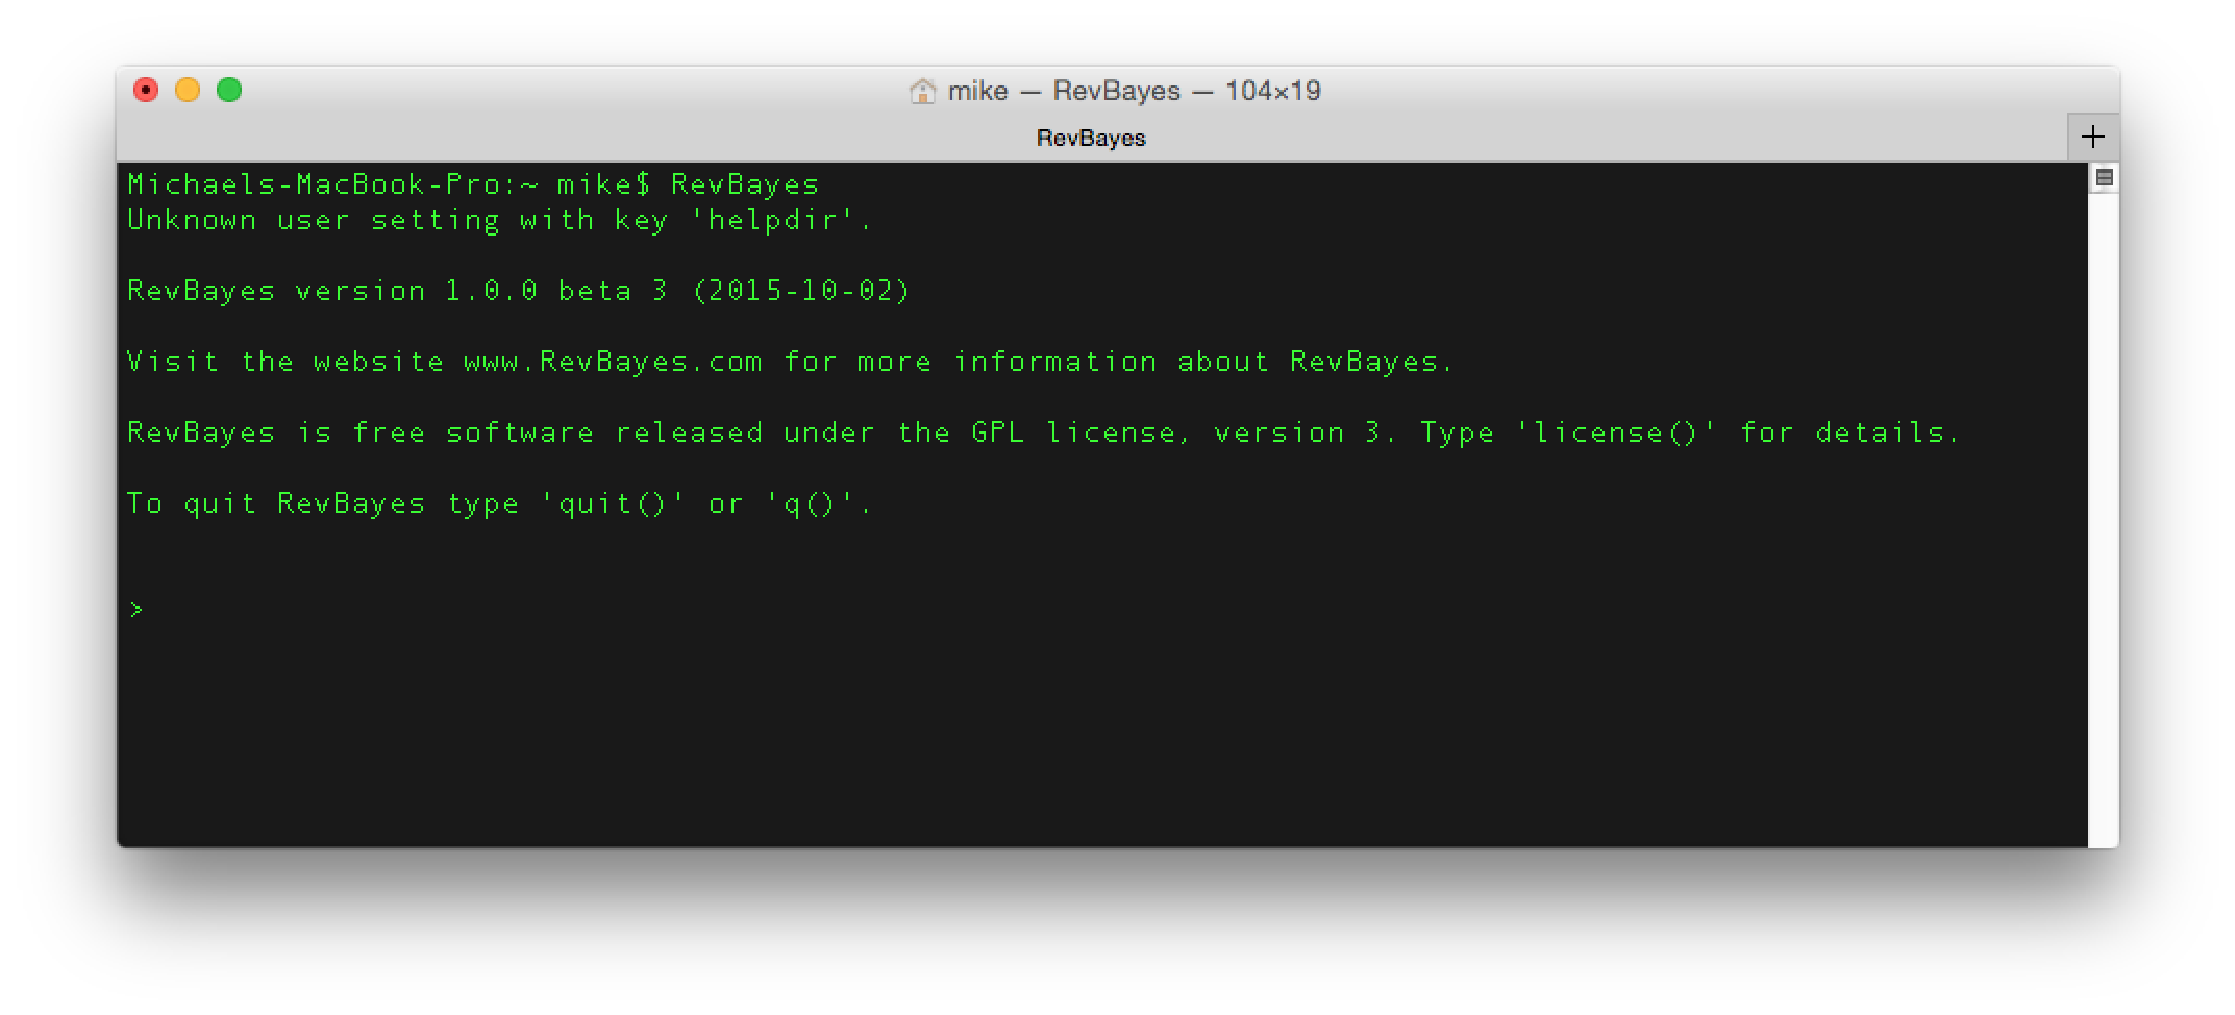
\includegraphics[width=\linewidth]{\ResourcePath figures/terminal.pdf}
\end{figure}

\subsection{Operators and Functions}

\Rev is an interpreted language for statistical computing and phylogenetic analysis.
Therefore, the basics are simple mathematical operations.
Entering each of the following lines will automatically execute these operations.
{\tt \begin{snugshade*}
\begin{lstlisting}    
# Simple mathematical operators:
1 + 1                            # Addition
10 - 5                           # Subtraction
5 * 5                            # Multiplication
10 / 2                           # Division
2^3                              # Exponentiation
5%2                              # Modulo
\end{lstlisting}
\end{snugshade*}}

\begin{figure}[H]
	\centering
	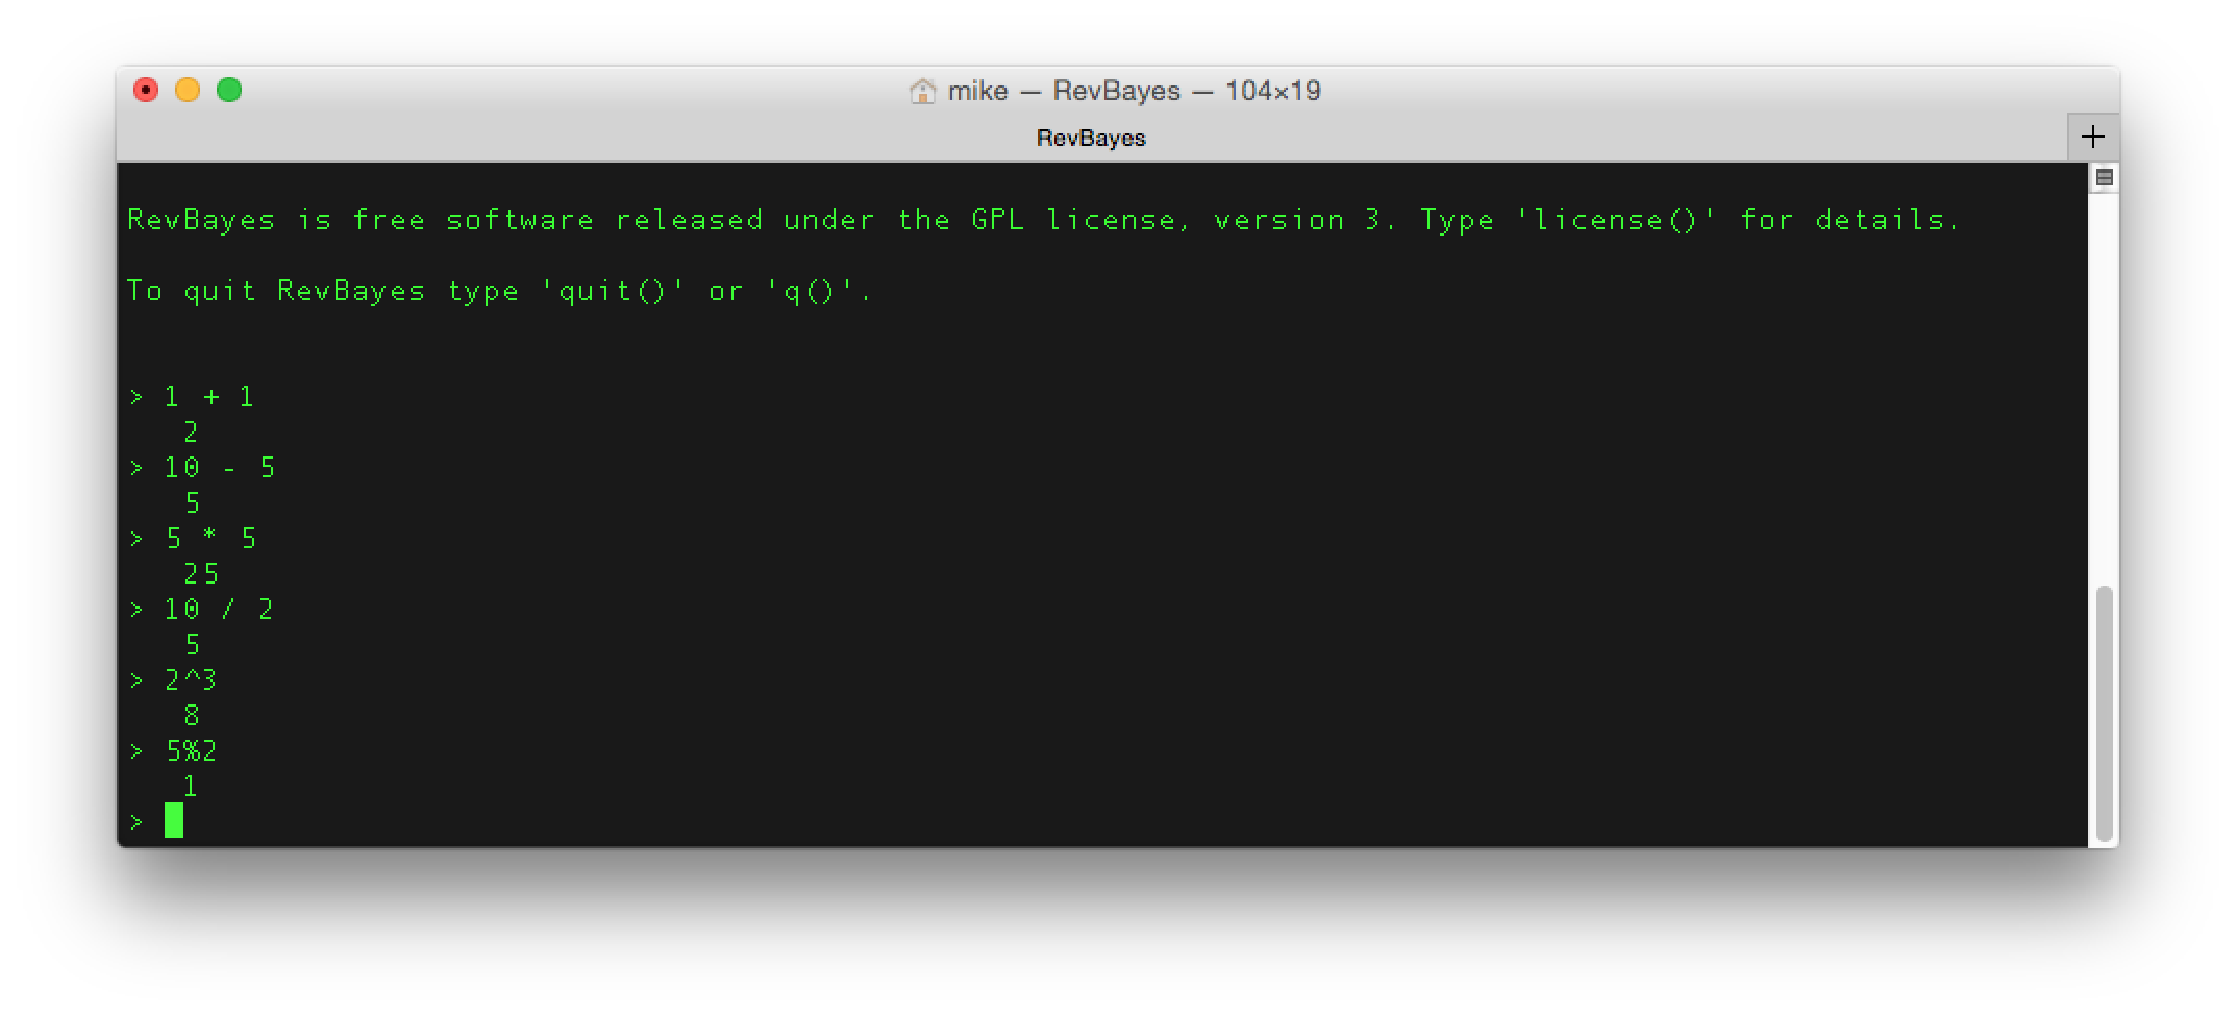
\includegraphics[width=\linewidth]{\ResourcePath figures/revbayes_operations.pdf}
\end{figure}
\noindent From now on, we will omit images of the terminal.

Each set of operations constitutes a \emph{statement}.
As you work through these tutorials, it is helpful to write the statements you enter into a blank text file, then copy-and-paste the statements into \Rev to execute them.
This way, you have a complete history of everything you've done, and can easily start over without having to rewrite everything.
We refer to the text file containing the list of commands as a \emph{script}, because it describes line-by-line instructions for the program to follow.

You can write multiple statements in the same line if you separate them by a semicolon (\texttt{;}).
The statements will execute as if you wrote each on a single line.
{\tt \begin{snugshade*}
\begin{lstlisting}    
1 + 1; 2 + 2                    # Multiple statements in one line
\end{lstlisting}
\end{snugshade*}}

Here you can see that comments always start with the hash symbol (\texttt{\#}).
Everything after the `\texttt{\#}'-symbol will be ignored.
In addition to these simple mathematical operations, \Rev provides some standard math functions which can be called by:
{\tt \begin{snugshade*}
\begin{lstlisting}    
# Math functions
exp(1)                           # exponential function
ln(1)                            # logarithmic function with natural base
sqrt(16)                         # square root function 
power(2,2)                       # power function: power(a,b) = a^b
\end{lstlisting}
\end{snugshade*}}
Notice that \Rev is case-sensitive.
That means, \Rev distinguishes upper and lower case letter for both variable names and function names.
For example, only the first of these two calls will work:
{\tt \begin{snugshade*}
\begin{lstlisting}    
exp(1)                           # correct lower case name
Exp(1)                           # wrong upper case name
\end{lstlisting}
\end{snugshade*}}

%\clearpage
\subsection{Variable Declaration and Assignment}
One of the most important features of \RevBayes (or any programming language, really) is the ability to declare and assign variables.
Variables store information to be referenced later, and can change throughout the execution of the program.
There are three kinds of variables in \RevBayes, called \emph{constant}, \emph{deterministic}, and \emph{stochastic} variables.
Constant variables contain values that are not random in your model.
Deterministic variables are functions of other variables.
Stochastic variables are random variables in your model, and will change during your analysis; importantly, stochastic variables (being random variables) are always associated with a particular statistical distribution.

Different types of variables differ in how you create them and assign values to them.
We will begin by creating a constant variable with name \texttt{a} that starts with the value 1. 
The left arrow assignment (\texttt{<-}) always creates a constant variable, and automatically assigns the following value to it.
{\tt \begin{snugshade*}
\begin{lstlisting}    
# Variable assignment: constant
a <- 1                           # assignment of constant node `a'
\end{lstlisting}
\end{snugshade*}}
You see the value of `a' by just typing in the variable name and pressing enter.
{\tt \begin{snugshade*}
\begin{lstlisting}    
a                                # printing the value of `a'
\end{lstlisting}
\end{snugshade*}}

Next, we create a deterministic variable \texttt{b} using the \texttt{:=} assignment computed by \texttt{exp(a)} and another deterministic variable \texttt{c} computed by \texttt{ln(b)}. 
Deterministic variables are always created using the colon-equal assignment (\texttt{:=}). 

{\tt \begin{snugshade*}
\begin{lstlisting}    
# Variable assignment: deterministic

# assignment of deterministic node `b' with
# the exponential function with parameter `a'
b := exp(a)  
b

# assignment of deterministic node `c' with
# logarithmic function with parameter `b'
c := ln(b)              
c 
\end{lstlisting}
\end{snugshade*}}

Finally, we will create the third type of variables in \Rev: stochastic variables.
We will create a random variable \texttt{x} from an exponential distribution with parameter \texttt{lambda}.  
Stochastic assignments use the $\sim$ operation.
{\tt \begin{snugshade*}
\begin{lstlisting}     
# Variable assignment: stochastic

# assign constant node `lambda' with value `1'
lambda <- 1.0

# create stochastic node with exponential 
# distribution and parameter `lambda'
x ~ dnExponential(lambda)
\end{lstlisting}
\end{snugshade*}}
The value of \texttt{x} is a random draw from the distribution. 
You can see the value and the probability (or log-probability) of the current value under the current parameter values by
{\tt \begin{snugshade*}
\begin{lstlisting}    
x                                # print value of stochastic node `x'
x.probability()                  # print the probability if `x'
x.lnProbability()                # print the log-probability if `x'
\end{lstlisting}
\end{snugshade*}}



\subsection{Distributions and Random Numbers}

\Rev provides functions for common statistical distributions.
We'll demonstrate by generating random exponential numbers as we did in lecture.
Recall that we can transform a random variable $u$ sampled from a Uniform(0,1) distribution into an exponential distribution with rate parameter $\lambda$:
\begin{align*}
	u &\sim \text{Uniform(0,1)}\\
	x &= -\frac{1}{\lambda \ln u}
\end{align*}
In \Rev, we might describe $u$ as a stochastic variable, and $x$ as a deterministic variable (since it is a function of $u$):
{\tt \begin{snugshade*}
\begin{lstlisting}
# create the random variable u
u ~ dnUniform(0,1)
u

# determine the rate parameter
lambda <- 1.0

# create x as a deterministic function of u
x := - 1 / lambda * ln(u)
x
\end{lstlisting}
\end{snugshade*}}
\noindent Alternatively, we can create $x$ directly as an exponential random variable:
{\tt \begin{snugshade*}
\begin{lstlisting}
# create the random variable x
x ~ dnExponential(lambda)
x
\end{lstlisting}
\end{snugshade*}}



\subsection{Vectors}
Individual variables can have more than one value.
Variables that have more than one value are called \emph{vectors}.
The simplest way to create a vector is like this:
{\tt \begin{snugshade*}
\begin{lstlisting}    
v <- v(1.0,2.0,3.0)              # create a vector
\end{lstlisting}
\end{snugshade*}}
\noindent You can refer to a specific value in the vector using brackets, \texttt{[i]}, where \texttt{i} is the index of the variable of interest.
{\tt \begin{snugshade*}
\begin{lstlisting}    
v[1]                             # print the first entry
v[1] <- 10                       # change the value of the first entry
v
\end{lstlisting}
\end{snugshade*}}



\subsection{\texttt{for} loops}
\texttt{for} loops are important programming structures that allow you to repeat the same statement a number of times on different variables.
The basic structure of a \texttt{for} loop is:
{\tt \begin{snugshade*}
\begin{lstlisting}    
# a for loop
for (<variable> in <set of values>) {
   <statements using variable>
}
\end{lstlisting}
\end{snugshade*}}
\noindent The \texttt{for} statement is followed by a set of parenthesis containing \texttt{<variable>}, which contains the name of the variable being iterated, and \texttt{<set of values>}, which are the values that the variable iterates over.
The \texttt{for} loop variable is a special variable that is created by the \texttt{for} loop: you do not have to create it before executing the loop.
This simple \texttt{for} loop creates the variable \texttt{i}, and for each value of \texttt{i} from 1 to 100, prints the value of \texttt{i} to the screen.
{\tt \begin{snugshade*}
\begin{lstlisting}    
for (i in 1:100) {
  i
}
\end{lstlisting}
\end{snugshade*}}

\noindent \texttt{for} loops are very powerful programming tools.
We can use a \texttt{for} loop to create an entire \emph{vector} of uniform random numbers, and transform them into a \emph{second} vector of exponential random numbers.
{\tt \begin{snugshade*}
\begin{lstlisting}    
for (i in 1:100) {
  u[i] ~ dnUniform(0,1)
  x[i] := - 1.0 / lambda * ln(u[i])
}
\end{lstlisting}
\end{snugshade*}}

\noindent Close \Rev using the statement \texttt{q()}.
{\tt \begin{snugshade*}
\begin{lstlisting}    
q()
\end{lstlisting}
\end{snugshade*}}

\subsection{References}

\bibliographystyle{sysbio}
\bibliography{\GlobalResourcePath refs}

\section{Exercises to the \RevBayes introduction}

\begin{enumerate}
\item Create a variable called $z$ with the value 10 (\texttt{z <- 10}). What kind of variable is this (constant, stochastic or deterministic)?

\bigskip
\TextField[name=var_type,backgroundcolor=TextFieldBackgroundColor,color=TextFieldTextColor,bordercolor=TextFieldBoxColor,height=1cm,width=\TextFieldWidth,multiline=true]{}
\bigskip

\item Create a second variable $y$ which is $y := f(z) := z ^ 2$. What kind of variable is $y$? What is its value?

\bigskip
\TextField[name=var_type_func,backgroundcolor=TextFieldBackgroundColor,color=TextFieldTextColor,bordercolor=TextFieldBoxColor,height=1cm,width=\TextFieldWidth,multiline=true]{}
\bigskip

\bigskip
\item Change the value of $z$ to 100. Before printing $y$, can you guess its value?

\bigskip
\TextField[name=z_value,backgroundcolor=TextFieldBackgroundColor,color=TextFieldTextColor,bordercolor=TextFieldBoxColor,height=1cm,width=\TextFieldWidth,multiline=true]{}

\bigskip
\item Write a \texttt{for} loop that creates 1000 random uniform numbers $u$ and 1000 exponential random numbers $x$ with $\lambda = 1$, as we did in the tutorial. Then, use the same random uniform numbers $u$ to create 1000 exponential numbers $y$ with $\lambda = 10$. Using the \texttt{mean()} function, compare the means of $x$ and $y$. Which has a greater mean? Write your code and answer!


\bigskip
\TextField[name=random_numbers,backgroundcolor=TextFieldBackgroundColor,color=TextFieldTextColor,bordercolor=TextFieldBoxColor,height=2cm,width=\TextFieldWidth,multiline=true]{}

\bigskip
\item Experiment with different values of $\lambda$. How does the mean of $x$ depend on $\lambda$?

\bigskip
\TextField[name=var_dependencies,backgroundcolor=TextFieldBackgroundColor,color=TextFieldTextColor,bordercolor=TextFieldBoxColor,height=2cm,width=\TextFieldWidth,multiline=true]{}

\end{enumerate}

	
%\end{enumerate}



\chapter{General Syntax of \Rev}
\def \ResourcePath {RB_Rev_Tutorial/}
\section{Basic \Rev Commands}

\subsection{Introduction}

This tutorial demonstrates the basic syntactical features of \RevBayes and \Rev and shows how to set up and perform an analysis on ``toy'' statistical models for linear regression. 
This tutorial focuses on explaining probabilistic graphical models and the language \Rev \citep{Hoehna2016b}.
A good reference for probabilistic graphical models for Bayesian phylogenetic inference is given in \cite{Hoehna2014b}.
The statistical examples are borrowed from a fourth year statistics course taught in the fall term 2011 at Stockholm University.

The first section of this tutorial involves 
\begin{enumerate}
\item Creating different types of variables.
\item Learning about functions. 
\end{enumerate}

Then we will see how to perform statistical inference using \RevBayes and \Rev  by implementing a Monte Carlo algorithm. 
Finally, we will see how \RevBayes 's built-in functions vastly simplify this inference task.

All of the files for this analysis are provided for you, and you can run these without significant effort using the \cl{source()} function in the \RevBayes console:
{\tt \begin{snugshade*}
\begin{lstlisting}
source("RevBayes_scripts/basics.Rev")
\end{lstlisting}
\end{snugshade*}}
Nevertheless, you will learn more if you type in the commands directly.

Let's start with the basic concepts for the interactive use of \RevBayes with \Rev (the language of \RevBayes). 
You should try to execute the statements step by step, look at the output and try to understand what and why things are happening. 
We start with some simple concepts to get familiar and used to \RevBayes. 
By now you should have executed \RevBayes and you should see the command prompt waiting for input. 
The best exercise is to write these statements exactly in \RevBayes. 

\Rev is an interpreted language for statistical computing and analyses in evolutionary biology. Therefore, the basics are simple mathematical operations, such as 
{\tt \begin{snugshade*}
\begin{lstlisting}    
# Simple mathematical operators:
1 + 1                            # Addition
10 - 5                           # Subtraction
5 * 5                            # Multiplication
10 / 2                           # Division
2^3                              # Exponentiation
5%2                              # Modulo
\end{lstlisting}
\end{snugshade*}}
Just as a side note, you can also write multiple statements in the same line if you separate these by a semicolon (\cl{;}).
The statements will be executed as if you wrote each on a single line.
{\tt \begin{snugshade*}
\begin{lstlisting}    
1 + 1; 2 + 2                    # Multiple statements in one line
\end{lstlisting}
\end{snugshade*}}
    
Here you can see that comments always start with the hash symbol (\cl{\#}). 
Everything after the `\cl{\#}'-symbol will be ignored.
In addition to these simple mathematical operations, we provide some standard math functions which can be called by:
    
{\tt \begin{snugshade*}
\begin{lstlisting}    
# Math-Functions
exp(1)                           # exponential function
ln(1)                            # logarithmic function with natural base
sqrt(16)                         # square root function 
power(2,2)                       # power function: power(a,b) = a^b
\end{lstlisting}
\end{snugshade*}}
Notice that \Rev is case-sensitive. That means, \Rev distinguishes upper and lower case letter for both variable names and function names. For example, only the first of these two calls will work
{\tt \begin{snugshade*}
\begin{lstlisting}    
exp(1)                           # correct lower case name
Exp(1)                           # wrong upper case name
\end{lstlisting}
\end{snugshade*}}
Moreover, we provide functions for the common statistical distributions.
{\tt \begin{snugshade*}
\begin{lstlisting}    
# distribution functions
dexp(x=1,lambda=1)       # exponential distribution density function
qexp(0.5,1)              # exponential distribution quantile function
rexp(n=10,1)             # random draws from an exponential distribution
dnorm(-2.0,0.0,1.0)      # normal distribution density function
rnorm(n=10,0,1)          # random draws from a normal distribution
\end{lstlisting}
\end{snugshade*}}
You may have noticed that we sometimes provided labels of the arguments and sometimes not. 
You can always provide the argument labels and then \RevBayes will match the arguments based on the labels.
{\tt \begin{snugshade*}
\begin{lstlisting}    
dnorm(x=0.5,mean=0.0,sd=1)       # normal distribution density function
\end{lstlisting}
\end{snugshade*}}
If you do not provide the argument labels, then \RevBayes  will match the arguments by the best fitting types and the order in which you provided the arguments.
{\tt \begin{snugshade*}
\begin{lstlisting}    
dnorm(0.5,0.5,1)         # correct order
dnorm(0.5,1,0.5)         # mismatched order
\end{lstlisting}
\end{snugshade*}}
You may provide also just some arguments with labels and leave the other arguments without labels.
{\tt \begin{snugshade*}
\begin{lstlisting}    
dnorm(0.0,x=0.5,sd=1)    # partially labeled
\end{lstlisting}
\end{snugshade*}}
If you do not remember what the parameter name or parameter names of a function are, then you can simply type in the function name and \RevBayes will tell you the possible parameters with their names.
{\tt \begin{snugshade*}
\begin{lstlisting}    
dnorm
\end{lstlisting}
\end{snugshade*}}

\subsection{Variable Declaration}
The next, and very important feature of \RevBayes, is variable declaration. 
We have three types of (model) variables, namely constant, deterministic and stochastic variables, which represent the same three types of DAG nodes. 
Here we show how to construct the different variables and how they behave differently. 
First, we focus on the difference between constant and deterministic variables.

Let us begin by creating a constant variable with name \cl{a} and assigned the value 1 to it. 
The left arrow assignment (\cl{<-}) always creates a constant variable.
{\tt \begin{snugshade*}
\begin{lstlisting}    
# Variable assignment: constant and deterministic
a <- 1                           # assignment of constant node 'a'
\end{lstlisting}
\end{snugshade*}}
You see the value of 'a' by just typing in the variable name and pressing enter.
{\tt \begin{snugshade*}
\begin{lstlisting}    
a                                # printing the value of 'a'
\end{lstlisting}
\end{snugshade*}}
If you want to see which type of variable (constant, deterministic or stochastic) 'a' has, then call the structure function for it.
{\tt \begin{snugshade*}
\begin{lstlisting}    
str(a)                           # printing the structure information of 'a'
|*   _variable     = a
|*   _RevType      = Natural
|*   _RevTypeSpec  = [ Natural, Integer, RevObject ]
|*   _value        = 1
|*   _dagType      = Constant DAG node
|*   _children     = [  ]
|*   .methods = void function ()
\end{lstlisting}
\end{snugshade*}}
% Maybe not all of the above info is shown anymore?  I see only _variable, _dagType, and _children.
An additional quite useful built-in function in \RevBayes  is the \cl{type} function which gives you only the type information of the variable and thus is a subset of the \cl{str} function.
{\tt \begin{snugshade*}
\begin{lstlisting}    
type(a)                          # printing the type information of 'a'
|*    Natural
\end{lstlisting}
\end{snugshade*}}
Next, we create a deterministic variable \cl{b} using the \cl{:=} assignment computed by \cl{exp(a)} and another deterministic variable \cl{c} computed by \cl{ln(b)}. 
Deterministic variables are always created using the colon-equal assignment (\cl{:=}). 

{\tt \begin{snugshade*}
\begin{lstlisting}    
b := exp(a)                      # assignment of deterministic node 'b' with the exponential function with parameter 'a'
b                                # printing the value of 'b'
c := ln(b)                       # assignment of deterministic node 'c' with logarithmic function with parameter 'b'
c                                # printing the value of 'c'
\end{lstlisting}
\end{snugshade*}}
Again, you see the type of the variable and additional information such as which the parents and children are by calling the structure function on it.
{\tt \begin{snugshade*}
\begin{lstlisting}    
str(b)                           # printing the structure information of 'b'
\end{lstlisting}
\end{snugshade*}}
For example, see the difference to the creation of variable 'd', which is a constant variable.
{\tt \begin{snugshade*}
\begin{lstlisting}    
d <- ln(b)                       # assignment of constant node 'd' with the value if the logarithmic function with parameter 'b'
d                                # printing the value of 'd'
str(d)                           # printing the structure information of 'd'
\end{lstlisting}
\end{snugshade*}}
Currently, the variables \cl{c} and \cl{d} have the same value. 
We can check this using the equal comparison (\cl{==}).
{\tt \begin{snugshade*}
\begin{lstlisting}    
e := (c == d)			
e
\end{lstlisting}
\end{snugshade*}}
Now, if we assign a new value to variable \cl{a}, then naturally the value of \cl{a} changes. 
This has the consequence that all deterministic variables that use 'a' as a parameter, i.e., the variable \cl{b}, change their value automatically too.
{\tt \begin{snugshade*}
\begin{lstlisting}    
a <- 2                           # reassignment of variable a; every deterministic node which has 'a' as a parameter changes its value
a                                # printing the value of 'a'
b                                # printing the value of 'b'
c                                # printing the value of 'c'
d                                # printing the value of 'd'
e
\end{lstlisting}
\end{snugshade*}}
Since variable \cl{d} was a constant variable it did not change its value. 
This also means that \cl{e} is now false.

Finally, we show you how to create the third type of variables in \Rev: the stochastic variables. 
We will create a random variable \cl{x} from an exponential distribution with parameter \cl{lambda}.  
Stochastic assignments use the \cl{\rbdn} operation.
{\tt \begin{snugshade*}
\begin{lstlisting}     
# Variable assignment: stochastic
lambda <- 1                      # assign constant node 'lambda' with value '1'
x ~ dnExponential(lambda)        # create stochastic node with exponential distribution and parameter 'lambda'
\end{lstlisting}
\end{snugshade*}}
The value of \cl{x} is a random draw from the distribution. 
You can see the value and the probability (or log-probability) of the current value under the current parameter values by
{\tt \begin{snugshade*}
\begin{lstlisting}    
x                                # print value of stochastic node 'x'
x.probability()                  # print the probability if 'x'
x.lnProbability()                # print the log-probability if 'x'
str(x)                           # printing all the information of 'x'
\end{lstlisting}
\end{snugshade*}}
Similarly, we create a random variable \cl{y} from a normal distribution by
{\tt \begin{snugshade*}
\begin{lstlisting}    
mu <- 0
sigma <- 1
y ~ dnNorm(mu,sigma)	
y.probability()                  # print the probability of 'y'
y.lnProbability()                # print the log-probability if 'y'
str(y)                           # printing all the information of 'y'
\end{lstlisting}
\end{snugshade*}}

Variables that are not part of a model are assigned with \cl{=}, for example, \cl{i = 0}.

Now you know everything there is about creating the different types of variables and the different ways in which these variables behave.



\subsubsection{Simple variable manipulation and other types of assignments}
\Rev provides some convenience variable manipulation operations that are equivalent to variable manipulations in other programming languages such as C/C++, Java and Python.
You can increment (\cl{++}) and decrement (\cl{-\,-}) a variable.
The increment operation increases the current value of a variable by 1 and the decrement operation decreases the value by 1.
A post increment (\cl{a++}) increases the value after returning the value, that is, the old value is returned.
A pre increment (\cl{++a}) increases the value before returning the value, that is, the new value is returned.
{\tt \begin{snugshade*}
\begin{lstlisting}    
index <- 1
index++                          # post increment
++index                          # pre increment
index--                          # post decrement
--index                          # pre decrement
\end{lstlisting}
\end{snugshade*}}
Additionally, you can use addition (\cl{a += b}), subtraction (\cl{a -= b}), multiplication (\cl{a *= b}) and division (\cl{a /= b}) to an existing variable.
{\tt \begin{snugshade*}
\begin{lstlisting}    
index += 10                      # add 10 to the current value
index *= 2                       # double the current value
\end{lstlisting}
\end{snugshade*}}
These variable manipulations will come in very handy for indices of vectors/arrays.

\subsubsection{Vectors}
Common values in \RevBayes are of scalar types.
That means that not everything is a vector by default.
Instead, you can create a vector using three different ways.
First, you can call the vector function.
{\tt \begin{snugshade*}
\begin{lstlisting}    
v <- v(1,2,3)                    # create a vector
\end{lstlisting}
\end{snugshade*}}
Interestingly, we can use the same name for a variable as for a function: the variable \cl{v} and the function \cl{v(\ldots)}.
Both will still be fully functional and our interpreter checks if you asked for a function or a variable.

Second, you can use the square bracket notation.
{\tt \begin{snugshade*}
\begin{lstlisting}    
w <- [1,2,3]                     # create a vector
\end{lstlisting}
\end{snugshade*}}
And third, you can implicitly create the vector by assigning elements.
{\tt \begin{snugshade*}
\begin{lstlisting}    
z[1] <-1                         # implicit creation of a vector
z[2] <-2                   
z[3] <-3                  
\end{lstlisting}
\end{snugshade*}} 
The implicit creation does not need to instantiate the variable beforehand.
There are other useful built-in functions that produce vectors.
{\tt \begin{snugshade*}
\begin{lstlisting}    
1:10                             # range function
rep(10,1)                        # replicate an element n times
seq(1,20,2)                      # built a sequence from a to b by c
\end{lstlisting}
\end{snugshade*}} 

Vectors in \Rev belong to the class of objects that have methods.
You  can call a member method by
{\tt \begin{snugshade*}
\begin{lstlisting}    
x.<method name>(<arguments>)                 
\end{lstlisting}
\end{snugshade*}} 
You have seen two methods previously, \cl{probability} and \cl{lnProbability}.
If you don't remember what the methods were called, or if this object has any member methods, then you can get these by
{\tt \begin{snugshade*}
\begin{lstlisting}    
v.methods()                 
\end{lstlisting}
\end{snugshade*}} 
In general, this is very, very useful.
So for a vector we can get the size --- the number of elements --- by calling its member function:
{\tt \begin{snugshade*}
\begin{lstlisting}    
v.size()                 
\end{lstlisting}
\end{snugshade*}} 


\subsubsection{Control Structures}
In this next part we will learn about control structures in \Rev. 
The first control structure that we will look at is the \cl{for} loop.
A \cl{for} loop executes a single statement or a block of statements.
{\tt \begin{snugshade*}
\begin{lstlisting}    
# loops
for (<variable> in <set of value>) <single statement>
 
for (<variable> in <set of value>) 
   <single statement>

for (<variable> in <set of value>) {
   <multiple statements>
   <multiple statements>
   <multiple statements>
}
\end{lstlisting}
\end{snugshade*}}
The statement(s) will be executed for each value of variable of the \cl{for} loop.
A simple example is a \cl{for} loop that computes the sum of a sequence.
{\tt \begin{snugshade*}
\begin{lstlisting}    
sum <- 0
for (i in 1:100) {
   sum <- sum + i
}
sum
\end{lstlisting}
\end{snugshade*}}
Another example using a \cl{for} loop is the computation of the \href{http://en.wikipedia.org/wiki/Fibonacci_number}{Fibonacci number} for a given integer. 
{\tt \begin{snugshade*}
\begin{lstlisting}    
# Fibonacci series using a for loop
fib[1] <- 1
fib[2] <- 1
for (j in 3:10) {
   fib[j] <- fib[j - 1] + fib[j - 2]
}
fib
\end{lstlisting}
\end{snugshade*}}
We could also compute the Fibonacci numbers using a \cl{while} loop.
The \cl{while} loop continues to execute the statement(s) until the condition is wrong.
{\tt \begin{snugshade*}
\begin{lstlisting}    
# Fibonacci series using a while loop
fib[1] <- 1
fib[2] <- 1
j <- 3
while (j <= 10) {
   fib[j] <- fib[j - 1] + fib[j - 2]
   j++
}
fib
\end{lstlisting}
\end{snugshade*}}

\subsubsection{User Defined Functions}
In \Rev you can write your own functions as well.
The syntax for writing a function is:
{\tt \begin{snugshade*}
\begin{lstlisting}    
function <return value type> <function name> (<list of arguments>) { <statements> }
\end{lstlisting}
\end{snugshade*}}
As a simple example, let's write a function that computes the square of a number.
We expect that the function takes in any real number.
The type of real number is \cl{Real}.
Since the square is always a positive real number, we choose the return to be \cl{RealPos}
{\tt \begin{snugshade*}
\begin{lstlisting}    
# simple square function
function RealPos square ( Real x ) { x * x }
\end{lstlisting}
\end{snugshade*}}
Now we can call our own function the same way as we call other already built-in functions in \RevBayes.
{\tt \begin{snugshade*}
\begin{lstlisting}    
a <- square(5.0)
a
\end{lstlisting}
\end{snugshade*}}
As an exercise, let's write a function that computes the factorial of a natural number.
{\tt \begin{snugshade*}
\begin{lstlisting}    
# function for computing the factorial
function Natural fac(i) {
   if (i > 1) {
      return i * fac(i-1)
   } else {
      return 1
   }
}
b <- fac(6)
b
\end{lstlisting}
\end{snugshade*}}
Here you see that within your own function you can call your function as well, which is commonly called recursive function calls.

Now let us write a recursive function for the sum of numbers which we computed before using a \cl{for} loop.
{\tt \begin{snugshade*}
\begin{lstlisting}    
# function for computing the sum
function Integer sum(Integer j) {
   if (j > 1) {
      return j + sum(j-1)
   } else {
      return 1
   }
}
c <- sum(100)
c
\end{lstlisting}
\end{snugshade*}}
We can do the same for our favorite example, the Fibonacci series.
{\tt \begin{snugshade*}
\begin{lstlisting}    
# function for computing the fibonacci series
function Integer fib(Integer k) {
   if (k > 1) {
      return fib(k-1) + fib(k-2)
   } else {
      return k
   }
}
d <- fib(6)
d
\end{lstlisting}
\end{snugshade*}}
Now that should be enough to get you going with our first example analyses.




\newpage
\FloatBarrier
\section{Exercise: Poisson Regression Model for Airline Fatalities}

This exercise will demonstrate how to approximate the posterior distribution of some parameters using a simple Metropolis algorithm. 
The focus here lies in the Metropolis algorithm, Bayesian inference, and model specification---but not in the model or the data. 
After completing this computer exercise, you should be familiar with the basic Metropolis algorithm, analyzing output generated from a MCMC algorithm, and performing standard Bayesian inference.

\subsection{Model and Data}
We will use the data example from \cite{Gelman2003}.
A summary is given in Table~\ref{tab:airlineFatalities}.
\begin{table}[!hbtp]
\caption{Airline fatalities from 1976 to 1985. Reproduced from \cite[][Table~2.2 on p.~69]{Gelman2003}.}
\label{tab:airlineFatalities}
\smallskip
\centering
\begin{tabular}{ l | r r r r r r r r r r }
  \hline                       
  Year & 1976 & 1977 & 1978 & 1979 & 1980 & 1981 & 1982 & 1983 & 1984 & 1985 \\
  Fatalities & 24 & 25 & 31 & 31 & 22 & 21 & 26 & 20 & 16 & 22\\
  \hline  
\end{tabular}
\end{table}

These data can be loaded into \RevBayes by typing:
{\tt \begin{snugshade*}
\begin{lstlisting}    
observed_fatalities <- v(24,25,31,31,22,21,26,20,16,22)
\end{lstlisting}
\end{snugshade*}}

The model is a \href{http://en.wikipedia.org/wiki/Poisson_regression}{Poisson regression} model with parameters $\alpha$ and $\beta$
\begin{equation*}
y \sim \text{Poisson}(\exp(\alpha+\beta*x))
\end{equation*} 
where $y$ is the number of fatal accidents in year $x$. 
For simplicity, we choose uniform priors for $\alpha$ and $\beta$.
\begin{eqnarray*}
\alpha & \sim & \text{Uniform}(-10,10)\\
\beta &  \sim & \text{Uniform}(-10,10)
\end{eqnarray*}
The probability density can be computed in \RevBayes for a single year by
{\tt \begin{snugshade*}
\begin{lstlisting}    
dpoisson(y[i],exp(alpha+beta*x[i]))
\end{lstlisting}
\end{snugshade*}}

\subsection{Problems}

\subsubsection{Metropolis Algorithm}%

The source file for this sub-exercise \cl{airline\_fatalities\_part1.Rev}.

Let us construct a Metropolis algorithm that simulates from the posterior distribution $P(\alpha,\beta|y)$. 
We will construct this algorithm explicitly, without using the high-level functions existing in \RevBayes  to perform MCMC. 
In the next section, we will repeat the same analysis, this time using the high-level functions.
(More background on MCMC is provided in the \href{https://github.com/revbayes/revbayes_tutorial/raw/master/tutorial_TeX/RB_MCMC_Intro_Tutorial/RB_MCMC_Intro_Tutorial.pdf}{Introduction to Markov Chain Monte Carlo Algorithms tutorial}.)
 
For simplicity of the calculations you can ``normalize'' the years, e.g. 
{\tt \begin{snugshade*}
\begin{lstlisting}    
x <- 1976:1985 - mean(1976:1985)
\end{lstlisting}
\end{snugshade*}}

A common proposal distribution for $\alpha^{\prime} \sim P(\alpha[i-1])$ is the normal distribution with mean $\mu = \alpha[i-1]$ and standard deviation $\sigma = \delta_\alpha$:
% \begin{equation}
% \alpha^{\prime} \sim \text{norm}(alpha[i-1],delta\_alpha)
% \end{equation}

{\tt \begin{snugshade*}
\begin{lstlisting}    
alpha_prime <- rnorm(1,alpha[i-1],delta_alpha)
\end{lstlisting}
\end{snugshade*}}
A similar distribution should be used for $\beta^{\prime}$. 
{\tt \begin{snugshade*}
\begin{lstlisting}    
delta_alpha <- 1.0
delta_beta <- 1.0
\end{lstlisting}
\end{snugshade*}}
After you look at the output of the MCMC (later), play around to find appropriate values for $\delta_{\alpha}$ and $\delta_{\beta}$.

Now we need to set starting values for the MCMC algorithm.
Usually, these are drawn from the prior distribution, but sometimes if the prior is very uninformative, then these parameter values result in a likelihood of 0.0 (or log-likelihood of -Inf).
{\tt \begin{snugshade*}
\begin{lstlisting}    
alpha[1] <- -0.01     # you can also use runif(-1.0,1.0)
beta[1] <- -0.01      # you can also use runif(-1.0,1.0)
\end{lstlisting}
\end{snugshade*}}
Next, create some output for our MCMC algorithm.
The output will be written into a file that can be read into \R or Tracer \citep{Rambaut2011}.
{\tt \begin{snugshade*}
\begin{lstlisting}    
# create a file output
write("iteration","alpha","beta",file="airline_fatalities.log")
write(0,alpha[1],beta[1],file="airline_fatalities.log",append=TRUE)
\end{lstlisting}
\end{snugshade*}}
Note that we need a first iteration with value 0 so that Tracer can load in this file.

Finally, we set up a \cl{for} loop over each iteration of the MCMC.
{\tt \begin{snugshade*}
\begin{lstlisting}    
for (i in 2:10000) {
\end{lstlisting}
\end{snugshade*}}
Within the \cl{for} loop we propose new parameter values.
{\tt \begin{snugshade*}
\begin{lstlisting}    
    alpha_prime <- rnorm(1,alpha[i-1],delta_alpha)[1]
    beta_prime <- rnorm(1,beta[i-1],delta_beta)[1]
\end{lstlisting}
\end{snugshade*}}
For the newly proposed parameter values we compute the prior ratio.
In this case we know that the prior ratio is 0.0 as long as the new parameters are within the limits.
{\tt \begin{snugshade*}
\begin{lstlisting}    
    ln_prior_ratio <- dunif(alpha_prime,-10.0,10.0,log=TRUE) + dunif(beta_prime,-10.0,10.0,log=TRUE) - dunif(alpha[i-1],-10.0,10.0,log=TRUE) - dunif(beta[i-1],-10.0,10.0,log=TRUE)
\end{lstlisting}
\end{snugshade*}}
Similarly, we compute the likelihood ratio for each observation.
{\tt \begin{snugshade*}
\begin{lstlisting}    
    ln_likelihood_ratio <- 0
    for (j in 1:x.size() ) {
       lambda_prime <- exp( alpha_prime + beta_prime * x[j] )
       lambda <- exp( alpha[i-1] + beta[i-1] * x[j] )
       ln_likelihood_ratio += dpoisson(observed_fatalities[j],lambda_prime) - dpoisson(observed_fatalities[j],lambda)
    }
    ratio <- ln_prior_ratio + ln_likelihood_ratio
\end{lstlisting}
\end{snugshade*}}
And finally we accept or reject the newly proposed parameter values with probability \cl{ratio}.
{\tt \begin{snugshade*}
\begin{lstlisting}    
    if ( ln(runif(1)[1]) < ratio) {
       alpha[i] <- alpha_prime
       beta[i] <- beta_prime
    } else {
       alpha[i] <- alpha[i-1]
       beta[i] <- beta[i-1]
    }
\end{lstlisting}
\end{snugshade*}}
Then we log the current parameter values to the file by appending the file.
{\tt \begin{snugshade*}
\begin{lstlisting}    
    # output to a log-file
    write(i-1,alpha[i],beta[i],file="airline_fatalities.log",append=TRUE)
 }
\end{lstlisting}
\end{snugshade*}}
As a quick summary you can compute the posterior mean of the parameters.
{\tt \begin{snugshade*}
\begin{lstlisting}    
mean(alpha)
mean(beta)
\end{lstlisting}
\end{snugshade*}}
You can also load the file into \R or Tracer to analyze the output.


In this section of the first exercise we wrote our own little Metropolis algorithm in \Rev.
This becomes very cumbersome, difficult and slow if we'ld need to do this for every model.
Here we wanted to show you only the basic principle of any MCMC algorithm.
In the next section we will use the built-in MCMC algorithm of \RevBayes.




\subsubsection{MCMC analysis using the built-in algorithm in \RevBayes}
Before starting with this new approach it would be good if you either start a new \RevBayes session or clear all previous variables using the \cl{clear} function.
Currently we may have some minor memory problems and if you get stuck it may help to restart \RevBayes.

We start by loading in the data to \RevBayes.
{\tt \begin{snugshade*}
\begin{lstlisting} 
observed_fatalities <- v(24,25,31,31,22,21,26,20,16,22)
x <- 1976:1985 - mean(1976:1985)
\end{lstlisting}
\end{snugshade*}}
Then we create the parameters with their prior distributions.
{\tt \begin{snugshade*}
\begin{lstlisting} 
alpha ~ dnUnif(-10,10) 
beta ~ dnUnif(-10,10)
\end{lstlisting}
\end{snugshade*}}
It may be good to set some reasonable starting values especially if you choose a very uninformative prior distribution.
If by chance you had starting values that gave a likelihood of -Inf, then \RevBayes will try several times to propose new starting values drawn from the prior distribution.
{\tt \begin{snugshade*}
\begin{lstlisting} 
# let us use reasonable starting value
alpha.setValue(0.0)
beta.setValue(0.0)
\end{lstlisting}
\end{snugshade*}}
Our next step is to set up the moves.
Moves are algorithms that propose new values and know how to reset the values if the proposals are rejected.
We use the same sliding window move as we implemented above by ourselves.
{\tt \begin{snugshade*}
\begin{lstlisting} 
mi <- 0
moves[mi++] = mvSlide(alpha)
moves[mi++] = mvSlide(beta)
\end{lstlisting}
\end{snugshade*}}
Then we set up the model.
This means we create a stochastic variable for each observation and clamp its value with the observed data.
{\tt \begin{snugshade*}
\begin{lstlisting} 
for (i in 1:x.size() ) {
    lambda[i] := exp( alpha + beta * x[i] )
    y[i] ~ dnPoisson(lambda[i])
    y[i].clamp(observed_fatalities[i])
}
\end{lstlisting}
\end{snugshade*}}
We can now create the model by pulling up the model graph from any variable that is connected to our model graph.
{\tt \begin{snugshade*}
\begin{lstlisting} 
mymodel = model( alpha )
\end{lstlisting}
\end{snugshade*}}
We also need some monitors that report the current values during the MCMC run.
We create two monitors, one printing all numeric non-constant variables to a file and one printing some information to the screen.
{\tt \begin{snugshade*}
\begin{lstlisting} 
monitors[1] = mnModel(filename="output/airline_fatalities.log",printgen=10, separator = "	")
monitors[2] = mnScreen(printgen=10, alpha, beta)
\end{lstlisting}
\end{snugshade*}}
Finally we create an MCMC object.
The MCMC object takes in a model object, the vector of monitors and the vector of moves.
{\tt \begin{snugshade*}
\begin{lstlisting} 
mymcmc = mcmc(mymodel, monitors, moves)
\end{lstlisting}
\end{snugshade*}}
On the MCMC object we call its member method \cl{run} to run the MCMC.
{\tt \begin{snugshade*}
\begin{lstlisting} 
mymcmc.run(generations=3000)
\end{lstlisting}
\end{snugshade*}}
And now we are done {\LARGE \smiley}


\subsubsection{Posterior Distribution of $\alpha$ and $\beta$}
 
Report the posterior mean and 95\% credible intervals for $\alpha$ and $\beta$. 
Additionally, plot the posterior distribution of $\alpha$ and $\beta$ by plotting a histogram of the samples. 
% You can use the \R function
% \RCode{
% hist(alpha,nclass=20)
% }
%For more information consult the \R help about the histogram function. To export the figure you need to use commands similar to
%\RCode{
%png("myFigure.png")
%}
%then your commands for printing the figure (e.g. hist(alpha,nclass=20)) and then
%\RCode{
%dev.off()
%}

Plot the curve of $m(x) = \text{E}[\exp(\alpha+\beta*x)|y]$ for $x = [1976,1985]$. 
You can generate draws from the posterior distribution of the expected value for a specific $x$ by recording the current expected value at a iteration $i$ of the Metropolis algorithm $m\_sample(x)[i] = \text{E}[\exp(\alpha[i]+\beta[i]*x)|y]$ and taking the mean of those samples (\cl{m(x) = \text{mean}(m\_sample(x))}) afterwards. Since \RevBayes provides you with the samples of $m(x) = \text{E}[\exp(\alpha+\beta*x)|y] = \lambda_x$ you can simply plot these posterior curves.
 
%A plot of the posterior mean curve $m(x)=E(\exp(\alpha+\beta*x)|y)$ over a suitable range. 
%A few draws from the posterior curve, i.e. \cl{exp(alpha[i]+beta[i]*x)} for a few i:s would also be nice.
%(These are somewhat cumbersome to do in R, you may need to present sample code).

 
Produce a histogram of the predictive distribution of the number of fatalities in 2014 and estimate the posterior mean. 
The predictive distribution can be approximated simultaneously with the Metropolis algorithm. 
This means, for any iteration $i$ you simulate draws from the conditional distribution for $x = 2014$ and the current values of $\alpha[i]$ and $\beta[i]$.
 
Estimate the distribution of the mean of the posterior predictive distribution of the the number of fatalities in 2014. 
Therefore, let us denote the expected value of the posterior distribution by $\mu$. 
Since we do not know this value $\mu$ exactly, we can follow the Bayesian approach and associate a probability for each value $m$ as being the true expected value of the posterior distribution, given the observations $y$ ($P(m = \mu|y)$).
You can approximate this distribution by recording the expected value for the number of fatalities in 2014 ($\text{E}[\exp(\alpha+\beta*x)|y]$) in each iteration $i$ of the Metropolis algorithm. 
Plot a histogram of the expected values, compute the mean of the expected values and compare it to the previously obtained estimate of the mean of the posterior predictive distribution.
 
Follow the same approach as for the posterior predictive distribution for $x = 2014$, but this time for $x = 2016$ and estimate the probability of no fatality.
 
 
 
 

\newpage
\FloatBarrier
\section{Exercise: Poisson Regression Model for Coal-mine Accidents}
 
We will analyze a dataset coal-mine accidents.
The values are the dates of major (more than 10 casualties) coal-mining disasters in the UK from 1851 to 1962. 


\subsection{A model for disasters}

A common model for the number of events that occur over a period of time is a Poisson process, in which the numbers of events in disjoint time-intervals are independent and Poisson-distributed. 
We will discretize and look at the yearly number of accidents. 

In order to take into account the possible change of rate, we will allow for different rates before and after year $\theta$, where $\theta$ is unknown to us. 
Thus, the observation distribution of our model is 
$y_t \sim Poisson(\lambda_t)$ with $t = 1851,\ldots,1962$ and
\begin{eqnarray*}
\lambda_t & = & \begin{cases}
\beta & \mbox{if } t < \theta \\
\gamma & \mbox{if } t \geq \theta
\end{cases}
\end{eqnarray*}
Thus, the rate $\lambda_t$ is defined by three unknown parameters: $\beta$, $\gamma$ and $\theta$. A hierarchical choice of priors is given by
\begin{eqnarray*}
 \eta & \sim & Gamma(10.0;20.0) \\ 
 \beta & \sim & Gamma(2.0;\eta) \\
 \gamma & \sim &Gamma(2.0;\eta) \\
 \theta & \sim & Uniform(1852,\ldots,1962)
\end{eqnarray*}
which brings an additional parameter $\eta$ in the model. 
For $\theta$ we have used a uniform prior over the years, but excluded year 1851 in order to make sure at least one year has rate $\beta$.
The hierarchical prior carries the belief that $\beta$ and $\gamma$ are somewhat similar in size,
since they both depend on $\eta$. 

\subsection*{The model in \Rev}

We start as usual by loading in the data.
{\tt \begin{snugshade*}
\begin{lstlisting} 
observed_fatalities <-  v(4, 5, 4, 1, 0, 4, 3, 4, 0, 6, 3, 3, 4, 0, 2, 6, 3, 3, 5, 4, 5, 3, 1, 4, 4, 1, 5, 5, 3, 4, 2, 5, 2, 2, 3, 4, 2, 1, 3, 2, 2, 1, 1, 1, 1, 3, 0, 0, 1, 0, 1, 1, 0, 0, 3, 1, 0, 3, 2, 2, 0, 1, 1, 1, 0, 1, 0, 1, 0, 0, 0, 2, 1, 0, 0, 0, 1, 1, 0, 2, 3, 3, 1, 1, 2, 1, 1, 1, 1, 2, 3, 3, 0, 0, 0, 1, 4, 0, 0, 0, 1, 0, 0, 0, 0, 0, 1, 0, 0, 1, 0, 1)
year <- 1851:1962
\end{lstlisting}
\end{snugshade*}}
In \Rev we specify this prior choice by
{\tt \begin{snugshade*}
\begin{lstlisting} 
eta ~ dnGamma(10.0,20.0)
beta ~ dnGamma(2.0,eta)
gamma ~ dnGamma(2.0,eta)
theta ~ dnUnif(1852.0,1962.0)
\end{lstlisting}
\end{snugshade*}}
Then we select moves for each parameter.
For the rate parameters --- which are defined only on the positive real line --- we choose a scaling move.
Only for \cl{theta} we choose the sliding window proposal.
{\tt \begin{snugshade*}
\begin{lstlisting} 
mi <- 0
moves[mi++] = mvScale(eta)
moves[mi++] = mvScale(beta)
moves[mi++] = mvScale(gamma)
moves[mi++] = mvSlide(theta)
\end{lstlisting}
\end{snugshade*}}
Then, we set up the model by computing the conditional rate of the Poisson distribution, creating random variables for each observation and attaching (clamping) data to the variables.
{\tt \begin{snugshade*}
\begin{lstlisting} 
for (i in 1:year.size() ) {
    rate[i] := ifelse(theta > year[i], beta, gamma)
    y[i] ~ dnPoisson(rate[i])
    y[i].clamp(observed_fatalities[i])
}
\end{lstlisting}
\end{snugshade*}}
Finally, we create the model object from the variables, add some monitors and run the MCMC algorithm.
{\tt \begin{snugshade*}
\begin{lstlisting} 
mymodel = model( theta )

monitors[1] = mnModel(filename="output/coal_accidents.log",printgen=10, separator = "	")
monitors[2] = mnScreen(printgen=10, eta, lambda, gamma, theta)

mymcmc = mcmc(mymodel, monitors, moves)

mymcmc.run(generations=3000)
\end{lstlisting}
\end{snugshade*}}




%\subsection*{Output analysis}
%
%Run the algorithm for say N = 10000 iterations or more. 
%
%a) In 1872, legislation on safety in mines was strengthened. 
%In 1878 and 1897 legislation on liability of employers for accidents was strengthened. Approximate the probability that the change occurred in the year after either of these changes (expect small numbers).
%b) How could the information given in a) be used to construct a prior for ?


%\subsection*{Posterior curves}

%We will now look at ways of visualising the posterior of the rate-function t, t =
%1851; : : : ; 1962. First we plot data together with a few posterior draws:
%par(mfrow=c(1,1))
%plot(year,y)
%I <- (1:10)*500
%for (i in I){
%points(c(1851,theta[i],1962),c(lambda[i],gamma[i],gamma[i]),type="s")
%}
%This gives a visual impression of the posterior uncertainty involved. As a point-estimate,
%we start with the mean curve, i.e. t ! m(t) = E(tjy). This can be approximated as
%follows
%t<-1851:1962
%for (i in 1:112){
%m[i]<-mean(lambda*(theta>=t[i])+gamma*(theta<t[i]))
%}
%and added to the plot in green
%lines(t,m,lwd=4,col="green")
%An alternative point-estimate of t is the mode, i.e. the curve that maximises the posterior probability. In order to find this you need the stored values of the log-posterior
%in lp: we want the index i that gives the largest lp[i]. This is provided in R by
%i <- which.max(lp)
%next, plot in red by
%points(c(1851,theta[i],1962),c(lambda[i],gamma[i],gamma[i]),type="s",lwd=4,col="red")


\bigskip
\subsection{Batch Mode}

If you wish to run this exercise in batch mode, the files are provided for you. 

You can carry out these batch commands by providing the file name when you execute the \cl{rb} binary in your unix terminal (this will overwrite all of your existing run files).
\exs{\cl{\$ rb RevBayes\_scripts airline\_fatalities\_part1.Rev}}
\exs{\cl{\$ rb RevBayes\_scripts airline\_fatalities\_part2.Rev}}
\exs{\cl{\$ rb RevBayes\_scripts coalmine\_accidents.Rev}}


\bibliographystyle{sysbio}
\bibliography{\GlobalResourcePath refs}


\chapter{Reading and manipulating data}
\def \ResourcePath {RB_Data_Tutorial/}
\include{RB_Data_Tutorial/RB_Data_Tutorial_content}



\part{Bayesian Inference and MCMC Simulation}

\chapter{Introduction to Markov chain Monte Carlo Algorithms using an Archery Example}
\def \ResourcePath {RB_MCMC_Archery_Tutorial/}

\section{Overview}\label{sect:Overview}

This tutorial is intended to provide a introduction to the basics of Markov chain Monte Caro (MCMC) using the  Metropolis-Hastings algorithm. This will provide a brief introduction to MCMC moves as well as prior distributions. We begin with a simple example of estimating the probability distribution of an archer's ability to shoot at a target, and the distance those arrows land from the center. We will simulate data using this example and attempt to estimate the posterior distribution using a variety of MCMC moves. 

\bigskip
\subsection{Requirements}\label{subsect:Overview-Requirements}

\subsubsection{Required Software}\label{subsub:Req-Software}
This tutorial requires that you download and install the latest release of \RevBayes \citep{Hoehna2017a}, which is available for Mac OS X, Windows, and Linux operating systems. 
Directions for downloading and installing the software are available on the program webpage:
%\begin{center}
\href{http://revbayes.com/}{http://revbayes.com}.
%\end{center} 

The exercise provided also requires additional programs for editing text files and visualizing output. 
The following are very useful tools for working with \RevBayes:
\begin{itemize}[noitemsep,topsep=0pt]
\item A good text editor -- if you do not already have one that you like, we recommend one that has features for syntax coloring, easy navigation between different files, line numbers, etc.
Good options include \href{http://www.sublimetext.com/}{\tt Sublime Text} or \href{https://atom.io/}{\tt Atom}, which are available for Mac OSX, Windows, and Linux.
\item \href{http://tree.bio.ed.ac.uk/software/tracer/}{\tt Tracer} -- for visualizing and assessing numerical parameter samples from \RevBayes
\end{itemize}


\section{Modeling an Archer's Shots on a Target}\label{sect:Exercise}

\begin{figure}[h!]
\centering
\fbox{%
\begin{minipage}{0.7\linewidth}\centering     
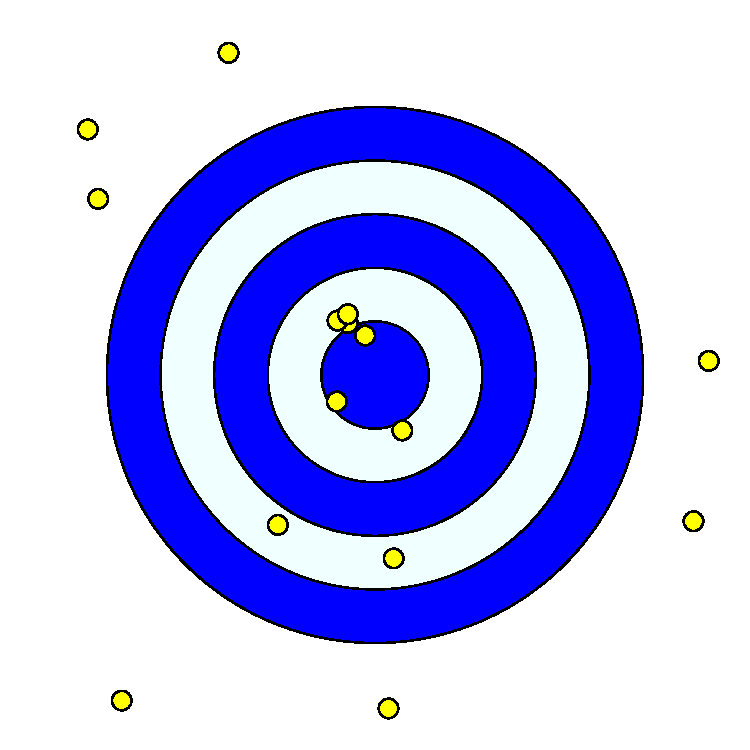
\includegraphics[width=2.25in,angle=0]{\ResourcePath figures/target.pdf}
\caption{Visual representation of the archery data used in this tutorial.
Each yellow dot represents the position of an arrow shot by an archer.
The distance of each arrow from the the center of the target is assumed to be exponentially distributed with mean $\mu$.}
\end{minipage}}
\label{fig:archery_model}
\end{figure}

We'll begin our exploration of Bayesian inference with a simple archery model.
For this model, there is an unknown archer shooting $n$ arrows at a target (Fig.\ \ref{fig:archery_model}). 
The distance $d$ of each arrow from the target's center is measured.
Let's assume that the distance of each arrow from the bullseye follows an exponential distribution---\IE $d\sim\mbox{Exp}(\mu^{-1})$.
This implies the archer has an inherent ability to shoot arrows at an average distance $\mu$.
Then, the probability density of each arrow distance $d_i$ is
\begin{align*}
P(d_i \mid \mu) = \frac{1}{\mu} e^{-d_i/\mu}
\end{align*}
Simple intuition suggests that, given that we observe $n$ arrows, a good estimate of $\mu$ is simply the average of all the arrow distances $\bar d = \frac{1}{n}\sum_{i=1}^n d_i$.
Indeed this is the maximum likelihood estimate!
In fact, given $n$ arrows whose distances follow an exponential distribution, it turns out that the observed average $\bar d$ follows a gamma distribution, with parameters $n$ and $n/\mu$.
\begin{align*}
P(\bar d \mid \mu,n) = \frac{(n/\mu)^n}{\Gamma(n)} {\bar d}^{n-1}e^{-n\bar d /\mu}
\end{align*}
In this case, the average $\bar d$ acts as a \emph{sufficient statistic} for $\mu$. This means that it tells just as much about $\mu$ as the collection of individual arrow distances.
Therefore, we will use a Gamma$(n, n/\mu)$ distribution on $\bar d$ as the likelihood of our data.

From Bayes' theorem, the \emph{posterior distribution} of $\mu$ given $\bar d$, $P(\mu \mid \bar d)$, is:
\begin{align*}
\overbrace{P(\mu \mid \bar d)}^{\text{posterior distribution}} = \frac{ \overbrace{P(\bar d \mid \mu)}^{\text{likelihood}} \times \overbrace{P(\mu)}^{\text{prior}}}{\underbrace{P(\bar d)}_{\text{marginal likelihood}}}
\end{align*}
The take-home message here is that, if we're interested in doing Bayesian inference for the archery model, we need to specify a \emph{likelihood function} and a \emph{prior distribution} for $\mu$.
In virtually all practical cases, we cannot compute the posterior distribution directly and instead use numerical procedures, such as a Markov chain Monte Carlo (MCMC) algorithm.
Therefore, we will also have to write a MCMC algorithm that samples parameter values in the frequency of their posterior probability.

We'll use a simple exponential distribution as a prior on the parameter of the model, $\mu$.
The \href{https://en.wikipedia.org/wiki/Exponential_distribution}{exponential distribution} has one parameter $\alpha$ representing our prior belief about the mean arrow distance (Figure~\ref{fig:exponential_distribution}).
Different choices for $\alpha$ represent different prior beliefs.
\begin{figure}[h!]
\centering 
\fbox{%
\begin{minipage}{0.7\linewidth}\centering    
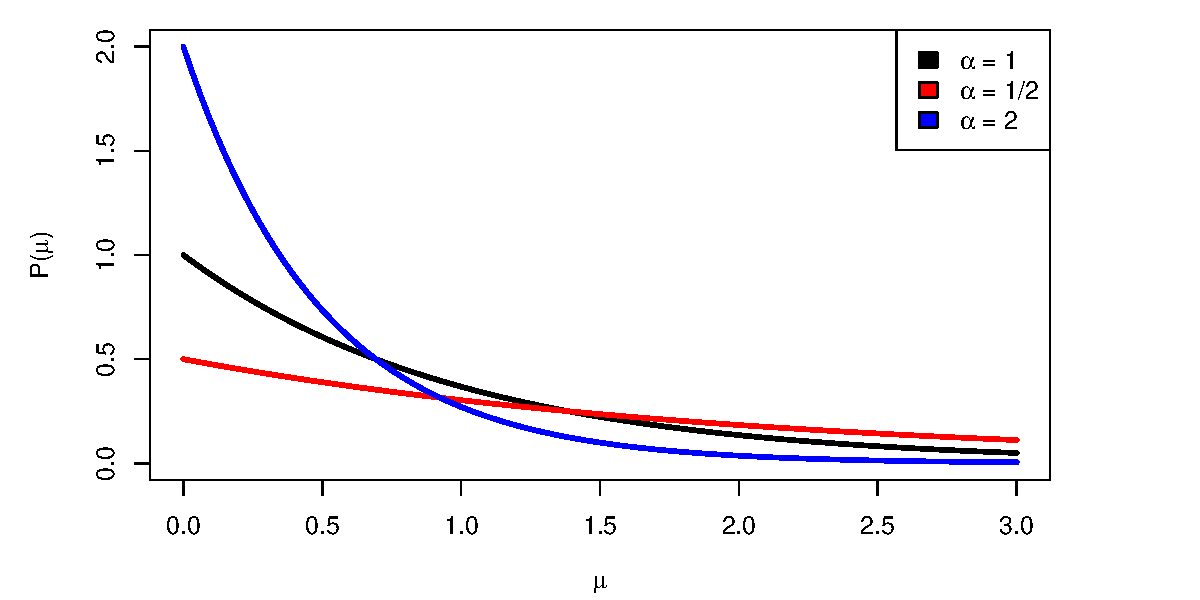
\includegraphics[width=0.7\linewidth,angle=0]{\ResourcePath figures/exp.pdf}
\caption{An exponential distribution with one parameter $\alpha$. This distribution is used as a prior distribution on the average arrow distance  $\mu$.
Here we show different curves for the exponential distribution when using different parameters.}
\end{minipage}}
\label{fig:exponential_distribution}
\end{figure}

Figure~\ref{fig:archery_model} shows the graphical model for the archery model.
This nicely visualizes the dependency structure in the model.
We see that the parameter $\alpha$ is drawn in a solid square, representing that this variable is constant (\IE it takes a ``known'' value).
Following the graph in figure~\ref{fig:archery_model}, we see an arrow connecting $\alpha$ and the variable $\mu$.
That simply means that $\mu$ depends on $\alpha$.
More specifically, $\mu$ is a stochastic variable (shown as a solid circle) that is drawn from an exponential distribution with parameter $\alpha$.
Another constant variable, $n$, represents the number of shots taken by the archer.
Finally, we have the observed data $\bar d$ which is drawn from a gamma distribution with parameters $\mu$ and $n$, as can be seen by the arrows pointing from those parameters to $d$.
Furthermore, the solid circle of $\bar d$ is shaded which means that the variable has data attached to it.
\begin{figure}[h!]
\centering
\fbox{%
\begin{minipage}{0.7\linewidth}\centering    
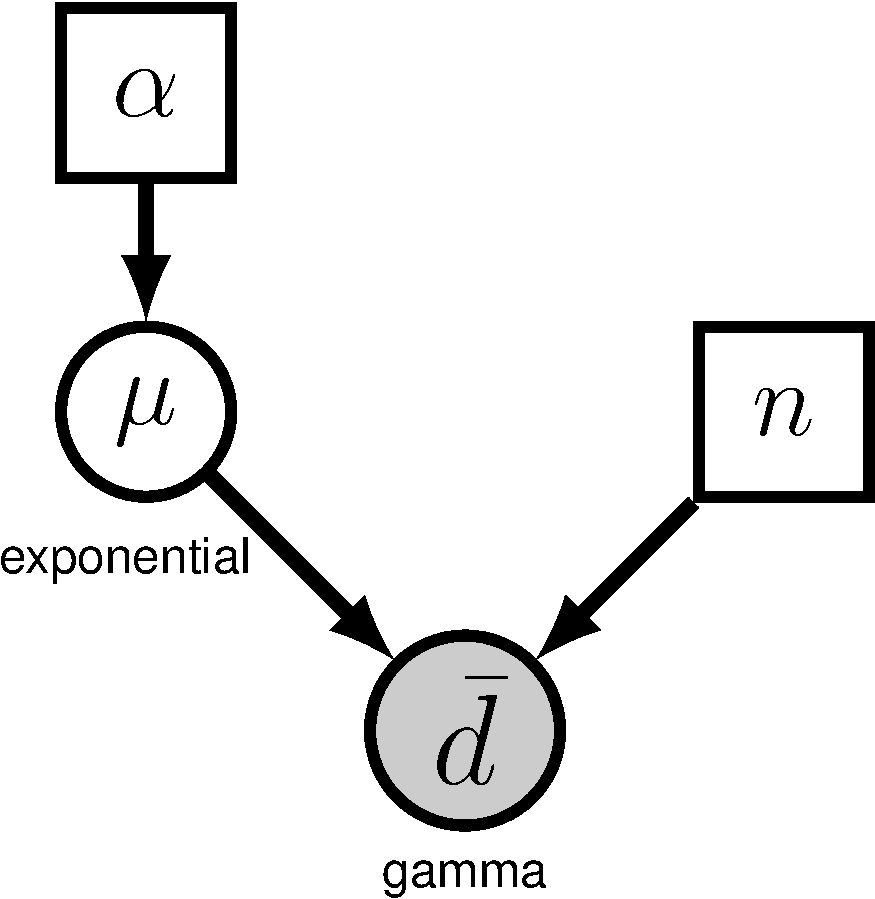
\includegraphics[width=1.8in,angle=0]{\ResourcePath figures/archery_graphical_model.pdf}
\caption{A graphical model for the archery model.}
\end{minipage}}
\label{fig:archery_model}
\end{figure}




\section{Writing MCMC from Scratch}\label{sect:MCMC-scratch}

\medskip
\subsection{Tutorial Format}\label{subsect:Exercise-Format}

This tutorial follows a specific format for issuing instructions and information.

{\begin{framed}
The boxed instructions guide you to complete tasks that are not part of the \RevBayes syntax, but rather direct you to create directories or files or similar.
\end{framed}}

Information describing the commands and instructions will be written in paragraph-form before or after they are issued.

All command-line text, including all \Rev syntax, are given in \cl{monotype font}. 
Furthermore, blocks of \Rev code that are needed to build the model, specify the analysis, or execute the run are given in separate shaded boxes.
For example, we will instruct you to create a new variable called \cl{n} that is equal to \cl{10} using the \cl{=} operator like this:
{\tt \begin{snugshade*}
\begin{lstlisting}
n = 10
\end{lstlisting}
\end{snugshade*}}

It is important to be aware that some PDF viewers may render some characters given as \colorbox{shadecolor}{\tt{Rev commands}} differently. 
Thus, if you copy and paste text from this PDF, you may introduce some incorrect characters. 
Because of this, we recommend that you type the instructions in this tutorial or copy them from the scripts provided (\href{https://github.com/revbayes/revbayes_tutorial/tree/master/RB_MCMC_Archery_Tutorial}{link}). 

\subsection{Create Your Script File}

%\impmark 
{\begin{framed}
Make yourself familiar with the example script called \href{https://raw.githubusercontent.com/revbayes/revbayes_tutorial/master/RB_MCMC_Archery_Tutorial/archery_MH.Rev}{\cl{archery\_MH.Rev}} which shows the code for the following sections. Then, start a new and empty script in your text editor and follow each step provided  as \colorbox{shadecolor}{\tt{Rev commands}} below.

Name the script file \cl{my\_archery\_MH.Rev} or anything you'd like.
\end{framed}}

\subsection{The Metropolis-Hastings Algorithm}\label{sect:MH_algorithm}
Though \RevBayes implements efficient and easy-to-use Markov chain Monte Carlo algorithms, we'll begin by writing one ourselves to gain a better understanding of the moving parts.
The Metropolis-Hastings MCMC algorithm \citep{Metropolis1953,Hastings1970} proceeds as follows:

\begin{enumerate}
	\item Generate initial values for the parameters of the model (in this case, $\mu$).
	\item Propose a new value (which we'll call $\mu^\prime$) for some parameters of the model, (possibly) based on their current values \label{sect:MH:step2}
	\item Calculate the acceptance probability, $R$, according to:
	\begin{align*}
		R = \text{min}\left\{1, \frac{P(\bar d \mid \mu^\prime)}{P(\bar d \mid \mu)} \times \frac{P(\mu^\prime)}{P(\mu)} \times \frac{q(\mu)}{q(\mu^\prime)} \right\}
	\end{align*}\label{sect:MH:step3}
	\item Generate a uniform random number $u$ between 1 and 0. 
%If it is less than $R$, accept the move (set $\mu = \mu^\prime$). Otherwise, keep the current value of $\mu$.
    \begin{description}
        \item [if $u<R$:] then accept the move and set $\mu = \mu^\prime$.
        \item [else (if $u\geq R$):] the value of $mu$ does not change and the move is rejected: $\mu = \mu$.
    \end{description}\label{sect:MH:step4}
	\item Record the values of the parameters.\label{sect:MH:step5}
	\item Return to step 2 many, many times, keeping track of the value of $\mu$.\label{sect:MH_alg:step6}
\end{enumerate}

\subsection{Reading in the data}
%Actually, in this case, we're just going to simulate some data on the spot.
Since we do not have access to archery data, we will simulate the the shots of our archer using the simulation tools in \RevBayes.
By simulating the data, we can also evaluate how well our moves and prior model perform---\IE how robust and accurate are our estimators.
After completing this exercise, feel free to repeat it and alter the true values to see how they influence the posterior distribution.
{\tt \begin{snugshade*}
\begin{lstlisting}    
# Simulate some data (i.e. shoot some arrows)
# First we need the number of arrows to shoot
n = 10
# Then we need a true mean distance
mu_true = 1
# Simulate the observed mean distance of the arrows shot from a gamma distribution
arrow_mean = rgamma(1, n, n/mu_true)[1]
\end{lstlisting}
\end{snugshade*}}

The \Rev code above uses the \cl{rgamma()} function to simulate a single observed \cl{arrow\_mean} from $n=10$ arrows shot on target.
The \cl{[1]} following the \cl{rgamma()} function is needed because this function always returns a {\emph vector} even when we only request a single value. Thus, in order to treat \cl{arrow\_mean} as a single value, we have to request the first element of the vector returned by that function.


\subsection{Initializing the Markov chain}
We have to start the MCMC off with some initial values for all of the parameters.
One way to do this is to randomly draw values of the parameters (just $\mu$, in this case) from the prior distribution.
We'll assume a simple exponential prior distribution; that is, one with $\alpha = 1$.
{\tt \begin{snugshade*}
\begin{lstlisting}
# Initialize the chain with some starting value
alpha = 1.0
mu = rexp(1, alpha)[1]
\end{lstlisting}
\end{snugshade*}}

%Now \cl{mu} is set to an initial value drawn from the exponential distribution. 


\subsubsection{Likelihood function}
Next we will specify the likelihood function, which will compute the probability of our data given the prior model.
We use the gamma distribution for the likelihood. Since the likelihood is defined only for values of $\mu$ greater than 0, we return a likelihood of 0.0 if $\mu$ is negative:
{\tt \begin{snugshade*}
\begin{lstlisting}
# Define the likelihood function on the mean 
function likelihood(mu){
    if(mu < 0.0)
        return 0.0

    return dgamma(arrow_mean, n, n/mu, log=false)
}
\end{lstlisting}
\end{snugshade*}}

In \Rev, we can create a {\em user-defined function} using the \cl{function} keyword. In our function definition above, \cl{likelihood()} takes a single value as an argument that is expected to be the mean ($\mu$) value.
All other parameters in our function are expected to be defined before \cl{likelihood()} is called.


\subsubsection{Prior distribution}
Similarly, we need to define a function for the prior distribution.
Here, we use the exponential probability distribution for the prior on $\mu$:
{\tt \begin{snugshade*}
\begin{lstlisting}    
# Define the prior function on the mean 
function prior(mu){
    if(mu < 0.0)
        return 0.0

    return dexp(mu, alpha, log=false)
}
\end{lstlisting}
\end{snugshade*}}



\subsubsection{Monitoring parameter values}
Additionally, we are going to monitor, \IE store, parameter values into a file during the MCMC simulation.
For this file we need to write the column headers in the first line of our output file, which we will name \cl{archery\_MH.log} (you may have to change the newline characters from \cl{"$\backslash$n"} to \cl{"$\backslash$r$\backslash$n"} if you're using a Windows operating system.):
{\tt \begin{snugshade*}
\begin{lstlisting}
# Prepare a file to log our samples
write("iteration","mu","\n",file="archery_MH.log")
write(0,mu,"\n",file="archery_MH.log",append=TRUE)
\end{lstlisting}
\end{snugshade*}}

We'll also monitor the parameter values to the screen, so let's print the initial values:
{\tt \begin{snugshade*}
\begin{lstlisting}
# Print the initial values to the screen
print("iteration","mu")
print(0,mu)
\end{lstlisting}
\end{snugshade*}}

\subsection{Writing the Metropolis-Hastings Algorithm}
At long last, we can write our MCMC algorithm.
First, we define how often we print to file (\IE monitor); this is called thinning if we do not choose to save every value of our parameter to file.
If we set the variable \cl{printgen=1}, then we will store the parameter values at every iteration; if we instead choose \cl{printgen=10}, then we'll only save the values every $10^{th}$ step in our Markov chain.
{\tt \begin{snugshade*}
\begin{lstlisting}
# Write the MH algorithm    
printgen = 10
\end{lstlisting}
\end{snugshade*}}
We will repeat this resampling procedure many times and iterate the MCMC using a \cl{for} loop (\EG step \ref{sect:MH_alg:step6} in Sect.\ \ref{sect:MH_algorithm}). 
We will start this part by defining the number of iterations for our MCMC (\cl{reps = 10000}) and writing the first line of our \cl{for} loop.
We'll also define a variable \cl{delta} (explained momentarily).
{\tt \begin{snugshade*}
\begin{lstlisting}
reps = 10000
delta = 1
for(rep in 1:reps){
\end{lstlisting}
\end{snugshade*}}
In \Rev, the contents of every \cl{for} loop must be enclosed within a set of  `curly braces' \cl{\{...\}}. Our loop will not be complete until we finish it and add the closing brace. 
Additionally, it is good style to make our loops readable by indenting the contents within the \cl{\{...\}}. 
We recommend that you use 4 spaces to represent these indents.

For our MCMC algorithm, the first thing we do is generate a new value of $\mu^\prime$ to evaluate (step \ref{sect:MH:step2} of Sect.\ \ref{sect:MH_algorithm}).
We'll propose a new value of $\mu$ by drawing a random number from a uniform window and then adding this random number to the current value (\IE centered on the previous value).
The value of \cl{delta} defines the width of the uniform window from which we draw new values.
Thus, if \cl{delta} is large, then the proposed values are more likely to be very different from the current value of $\mu$.
Conversely, if \cl{delta} is small, then the proposed values are more likely to be very close to the current value of $\mu$.
By changing the value of \cl{delta} we can tune the behavior of the proposal, and therefore \cl{delta} is called a \emph{tuning parameter}.
{\tt \begin{snugshade*}
\begin{lstlisting}    
    # Propose a new value of p
    mu_prime <- mu + runif(n=1,-delta,delta)[1]
\end{lstlisting}
\end{snugshade*}}

Next, we compute the proposed likelihood and prior probabilities using the functions we defined above, as well as the acceptance probability, $R$ (step \ref{sect:MH:step3} of Sect.\ \ref{sect:MH_algorithm}):
{\tt \begin{snugshade*}
\begin{lstlisting}    
    # Compute the acceptance probability
    R = ( likelihood(mu_prime)/likelihood(mu) ) * ( prior(mu_prime)/prior(mu) )
\end{lstlisting}
\end{snugshade*}}

Then, we accept the proposal with probability $R$ and reject otherwise (step \ref{sect:MH:step4} of Sect.\ \ref{sect:MH_algorithm}):
{\tt \begin{snugshade*}
\begin{lstlisting}    
    # Accept or reject the proposal
    u <- runif(1,0,1)[1]
    if(u < R){
        # Accept the proposal
        mu <- mu_prime
    }
\end{lstlisting}
\end{snugshade*}}

\pagebreak Finally, we store the current value of $\mu$ in our log file (step \ref{sect:MH:step5} of Sect.\ \ref{sect:MH_algorithm}).
Here, we actually check if we want to store the value during this iteration.
{\tt \begin{snugshade*}
\begin{lstlisting}
    if ( (rep % printgen) == 0 ) {
        # Write the samples to a file
        write(rep,mu,"\n",file="archery_MH.log",append=TRUE)
        # Print the samples to the screen
        print(rep,mu)
    }
} # end MCMC\end{lstlisting}
\end{snugshade*}}

\bigskip
\subsection{Execute the MCMC Analysis}\label{subsect:Exercise-RunMCMC}

Now that you have defined your model and written functions to compute the probability and sample values of $\mu$, you are now ready to run your analysis. 

{\begin{framed}
Begin by running the \RevBayes executable. 
You can do this by navigating to the folder containing your \RevBayes executable and running it. If you're on a Unix system you can do this by typing:

\colorbox{black}{\strut\hspace{1mm}\textcolor[rgb]{0,1,1}{\cl{./rb}}\hspace{0.925\textwidth}}

{\em Alternatively}, if you are on a Unix system and the \RevBayes binary is in your path, you only have to type the following from any directory:

\colorbox{black}{\strut\hspace{1mm}\textcolor[rgb]{0,1,1}{\cl{rb}}\hspace{0.925\textwidth}}
\end{framed}}

Now you can run your \RevBayes script:
{\tt \begin{snugshade*}
\begin{lstlisting}
source("my_archery_MH.Rev")
\end{lstlisting}
\end{snugshade*}}

\subsection{Exercise 1}

% TODO: I don't like how the "Step" goes into the margin (TAH)
\begin{enumerate}[label=\textnormal{Step \arabic*)},leftmargin=1.5cm]
	\item Write and execute the script outlined above, which you can give any name you like (there is also an example file called \cl{archery\_MH.Rev}).
	\item The \cl{.log} file will contain samples from the posterior distribution of the model. Open the file in \Tracer to learn about various features of the posterior distribution, for example: the posterior mean or the 95\% credible interval.
\end{enumerate}
Pretty awesome, right?

Below we show an example of the obtained output in \Tracer.
Specifically, Figure~\ref{fig:mcmc_samples} shows the sample trace (left) and the estimated posterior distribution of $\mu$ (right).
There are other parameters, such as the posterior mean and the 95\% HPD (highest posterior density) interval, that you can obtain from \Tracer.
\begin{figure}[h!]
\centering
\fbox{%
\begin{minipage}{\textwidth}\centering    
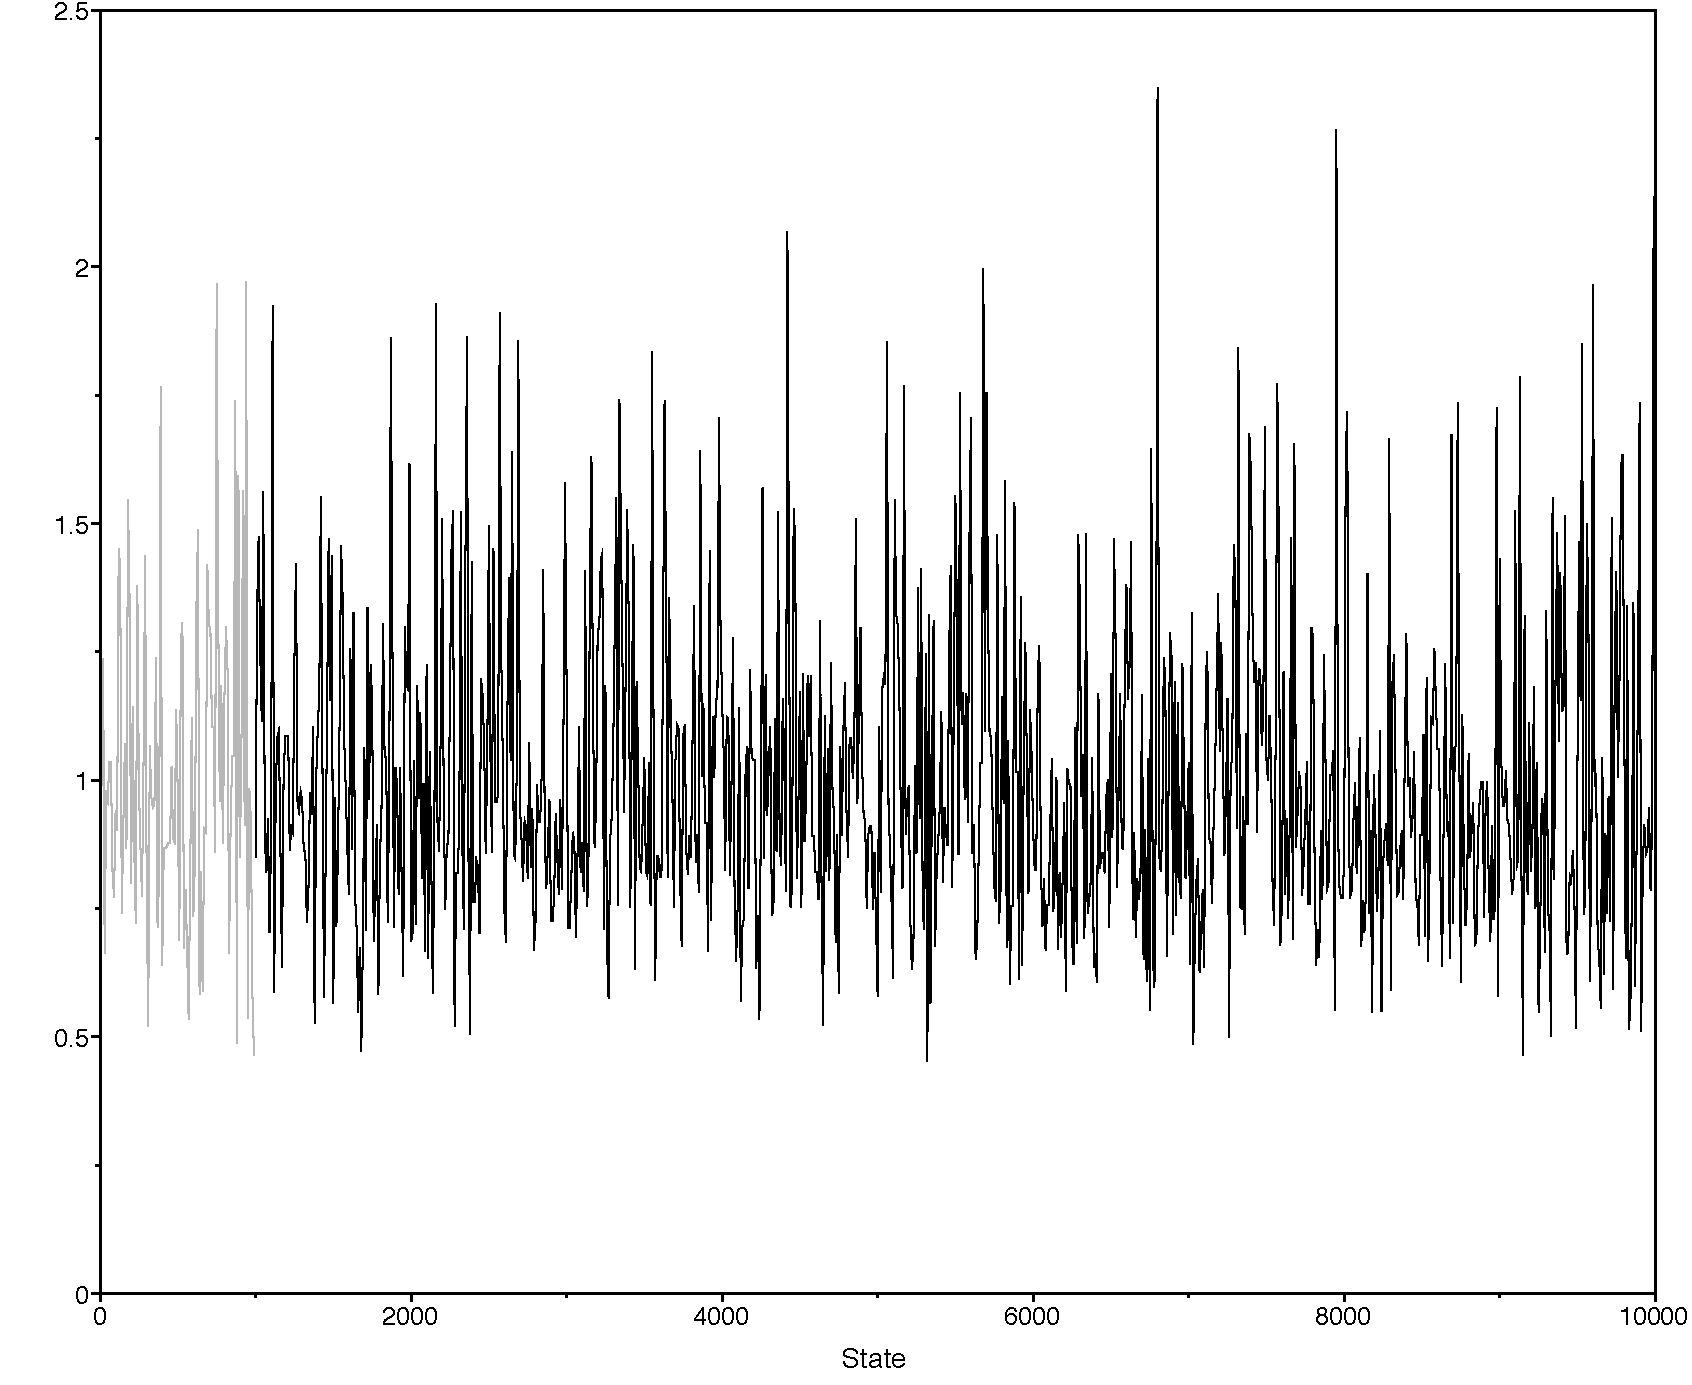
\includegraphics[width=0.45\linewidth,angle=0]{\ResourcePath figures/archery_MCMC_Trace.pdf}
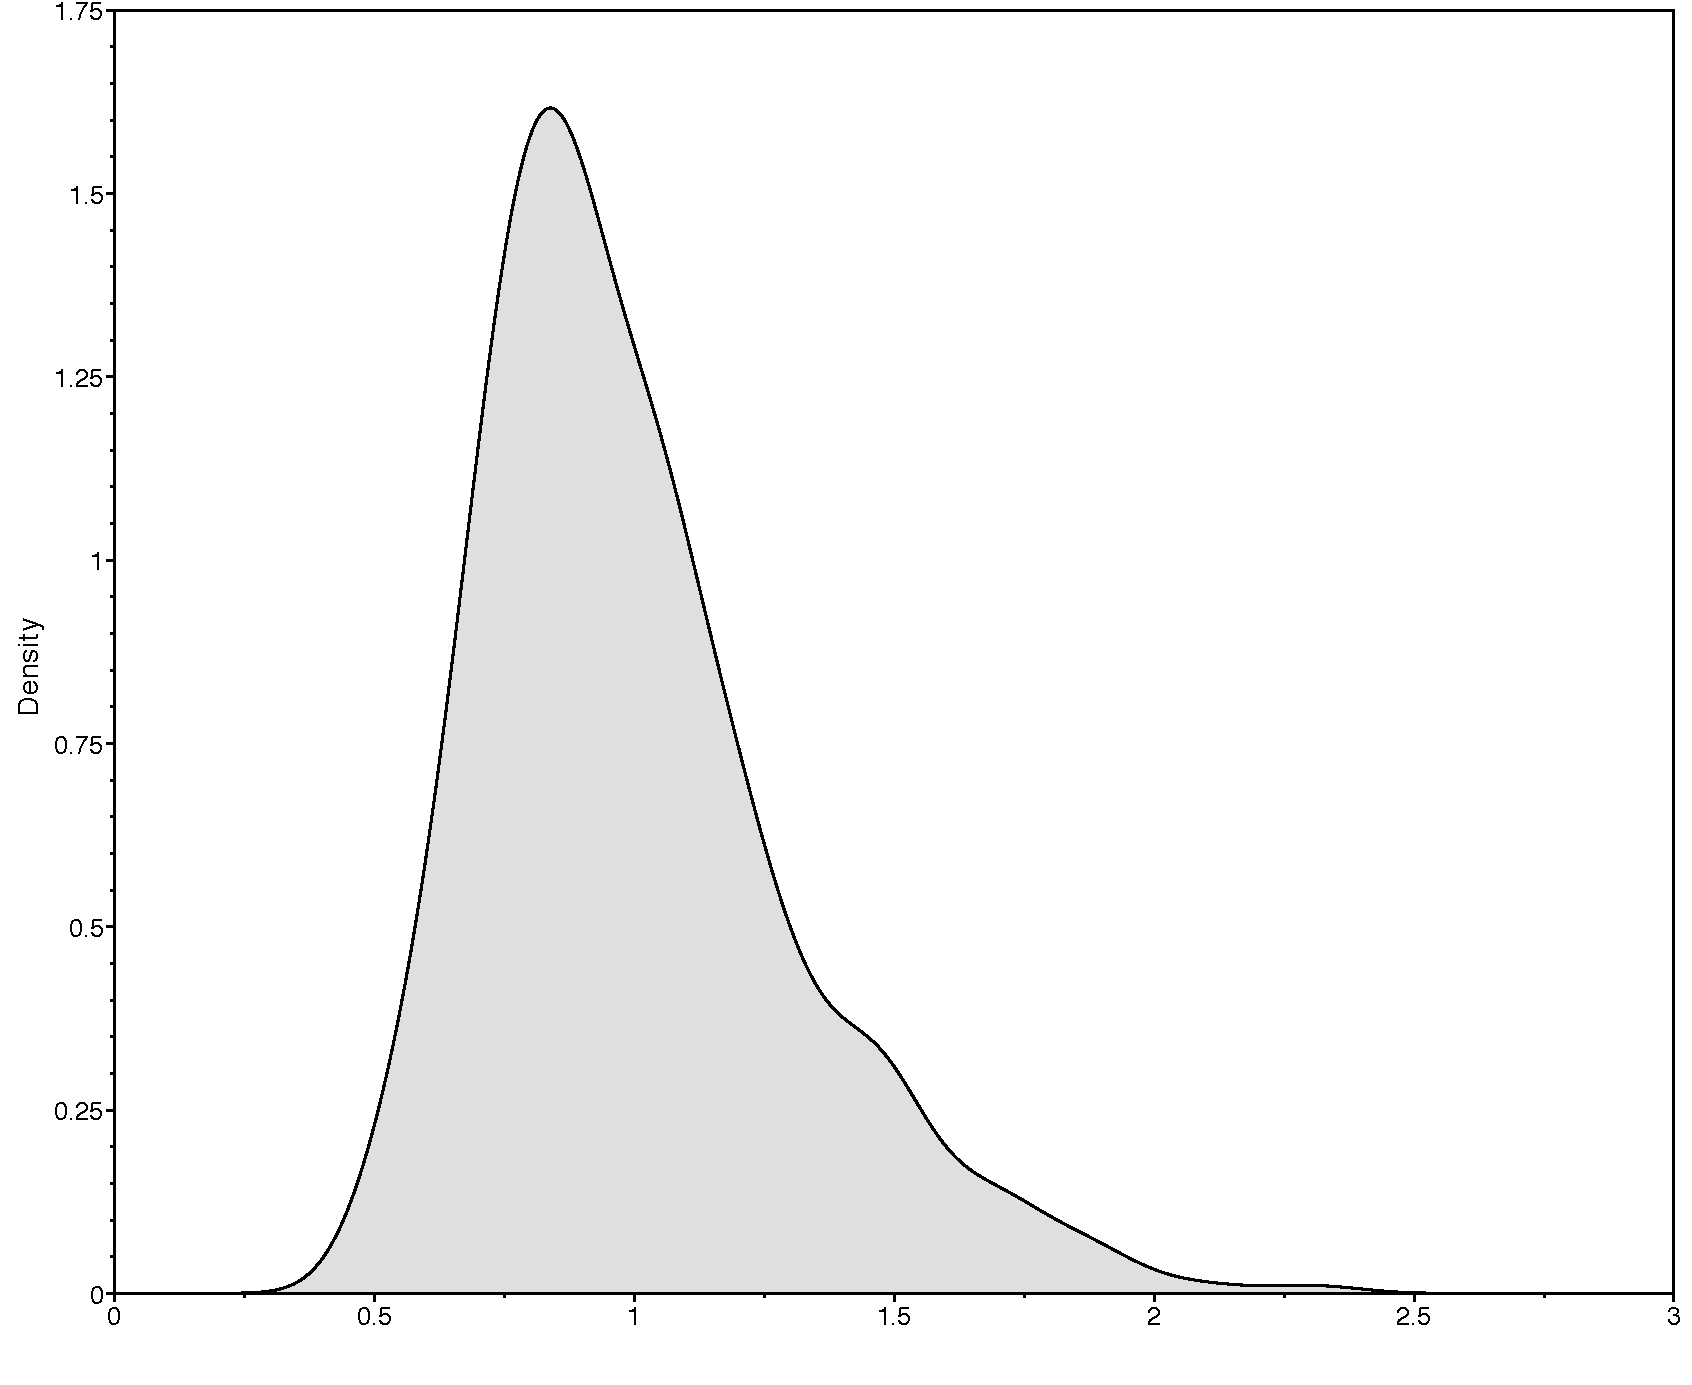
\includegraphics[width=0.45\linewidth,angle=0]{\ResourcePath figures/archery_MCMC_distribution.pdf}
\caption{Left: The \emph{Trace} of sample from an MCMC simulation. Right: The approximated posterior probability distribution for $\mu$.}
\end{minipage}}
\label{fig:mcmc_samples}
\end{figure}
\pagebreak


\section{More on Moves: Tuning and Weights}\label{sect:More_on_Moves}

In the previous example we hard coded a single move updating the variable $\mu$ by drawing a new value from a sliding window.
There are other ways how to propose new values; some of which are more efficient than others.

First, let us rewrite the MCMC loop so that instead we call a function, which we name \cl{move\_slide} for simplicity, that performs the move:
{\tt \begin{snugshade*}
\begin{lstlisting}    
for (rep in 1:reps){
    
    # call uniform move
    move_slide(1,1)
    
    if ( (rep % printgen) == 0 ) {
        # Write the samples to a file
        write(rep,p,"\n",file="archery_MH.log",append=TRUE)
        # Print the samples to the screen
        print(rep,mu)
    }

} # end MCMC
\end{lstlisting}
\end{snugshade*}}

\pagebreak\subsection{Slide move}
Now we need to actually write the \cl{move\_slide} function.
We mostly just copy the code we had before into a dedicated function
{\tt \begin{snugshade*}
\begin{lstlisting}    
function move_slide(delta, weight) {

    for (i in 1:weight) {
        # Propose a new value of mu
        mu_prime <- mu + runif(n=1,-delta,delta)[1]

        # Compute the acceptance probability
        R = ( likelihood(mu_prime)/likelihood(mu) ) * ( prior(mu_prime)/prior(mu) ) 

        # Accept or reject the proposal
        u = runif(1,0,1)[1] 
        if(u < R){
            # Accept the proposal
            mu = mu_prime 
        }
    }
} # end function
\end{lstlisting}
\end{snugshade*}}
There are a few things to consider in the function \cl{move\_slide}.
First, we do not have a return value because the move simply changes the variable $\mu$ if the move is accepted.
Second, in addition to the tuning parameter \cl{delta}, we expect an argument called \cl{weight} which will tell us how often we want to use this move.
Otherwise, this function does exactly the same what was inside the for loop previously.

(Note that you need to define this function before the for loop in your script).

%\impmark 
{\begin{framed}
Experiment with different values for \cl{delta} and check how the effective sample size (ESS) changes.
\end{framed}}

There is, {\it a priori}, no good method for knowing what values of \cl{delta} are most efficient.
However, there are some algorithms implemented in \RevBayes, called \emph{auto-tuning}, that will estimate good values for \cl{delta}.

\subsection{Scaling move}
As another move we will write a scaling move.
The scaling move proposes an update by drawing a random number from a Uniform(-0.5,0.5) distribution, exponentiating the random number, and then multiplying this scaling factor by the current value.
An interesting feature of this move is that it is not symmetrical and thus needs a Hastings ratio.
The Hastings ratio is rather trivial in this case, and one only needs to multiply the acceptance rate by the scaling factor.
{\tt \begin{snugshade*}
\begin{lstlisting}    
function move_scale(lambda, weight) {

    for (i in 1:weight) {
        # Propose a new value of p
        sf <- exp( lambda * ( runif(n=1,0,1)[1] - 0.5 ) )
        mu_prime <- mu * sf

        # Compute the acceptance probability
        R = ( likelihood(mu_prime)/likelihood(mu) ) * ( prior(mu_prime)/prior(mu) ) 

        # Accept or reject the proposal
        u = runif(1,0,1)[1] 
        if(u < R * sf){
            # Accept the proposal
            mu = mu_prime 
        }
    }
} # end function
\end{lstlisting}
\end{snugshade*}}
As before, this move has a tuning parameter called \cl{lambda}.

\begin{framed}
\IMPORANT The sliding-window and scaling moves are very common and popular moves in \RevBayes.
The code examples here are actually showing the exact same equation as implemented internally.
It will be very useful for you to understand these moves.	
\end{framed}


\subsection{Exercise 2}

\begin{enumerate}[label=\textnormal{Step \arabic*)},leftmargin=1.5cm]
	\item Rewrite your previous script to include these two different moves, and re-run the script to estimate the posterior distribution of $\mu$ again.
	\item Use only a single move and set \cl{printgen=1}. Which move has the best ESS?
	\item How does the ESS change if you use tuning parameter values \cl{delta=10} or \cl{delta=0.1} for the sliding-window move? What about \cl{lambda=10} or \cl{lambda=0.1} for the scaling move?
	\item You can keep track of your results using the following table.
\end{enumerate}
\begin{Form}
\begin{table}[h!]
\centering
\caption{\small Effective sample sizes (ESS) for two moves at three different tuning parameter values}
\resizebox{\textwidth}{!}{%
\begin{tabular}{l c c c c}
\hline
\textbf{Move} & \textbf{tuning = 10} & \textbf{tuning = 1} & \textbf{tuning = 0.1} \\ 
\hline
\vspace{1mm}
Sliding-window & \TextField[name=pp11,backgroundcolor={.85 .85 .85},color={0 0 1},height=3ex]{}  & \TextField[name=pp12,backgroundcolor={.85 .85 .85},color={0 0 1},height=3ex]{}  & \TextField[name=pp13,backgroundcolor={.85 .85 .85},color={0 0 1},height=3ex]{}\\
\hline
\vspace{1mm}
Scaling & \TextField[name=pp21,backgroundcolor={.85 .85 .85},color={0 0 1},height=3ex]{}  & \TextField[name=pp22,backgroundcolor={.85 .85 .85},color={0 0 1},height=3ex]{}  & \TextField[name=pp23,backgroundcolor={.85 .85 .85},color={0 0 1},height=3ex]{} \\
\hline
\end{tabular}}
\label{tab:pp}
\end{table}
\end{Form}

\section{The Metropolis-Hastings Algorithm with the \emph{Real} \RevBayes}
We'll now specify the exact same model in \Rev using the built-in modeling functionality and moves.
It turns out that the \Rev code to specify the above model is extremely simple and similar to the one we used before.
Again, we start by ``reading in'' (\emph{i.e.}, making up) our data.

{\tt \begin{snugshade*}
\begin{lstlisting}    
# Simulate some data (i.e. shoot some arrows)
# First we need the number of arrows to shoot
n = 10
# Then we need some true mean distance
mu_true = 1
# Simulate the observed mean distance of the arrows we shot
arrow_mean = rgamma(1, n, n/mu_true)[1]
\end{lstlisting}
\end{snugshade*}}

Now we specify our prior model.
{\tt \begin{snugshade*}
\begin{lstlisting}    
# Specify the prior distribution
alpha <- 1.0
mu ~ dnExponential(alpha)
\end{lstlisting}
\end{snugshade*}}

One difference between \RevBayes and the MH algorithm that we wrote above is that many MCMC proposals are already built-in, but we have to specify them \emph{before} we run the MCMC.
We usually define (at least) one move per parameter immediately after we specify the prior distribution for that parameter.

{\tt \begin{snugshade*}
\begin{lstlisting}    
# Define a move for our parameter, mu
moves[1] = mvSlide(mu, delta=1, weight=1.0)
\end{lstlisting}
\end{snugshade*}}

Next, our likelihood model.
{\tt \begin{snugshade*}
\begin{lstlisting}    
# Specify the likelihood model
d_bar ~ dnGamma(n, n/mu)
d_bar.clamp(arrow_mean)
\end{lstlisting}
\end{snugshade*}}

We wrap our full Bayesian model into one model object (this is a convenience to keep the entire model in a single object, and is more useful when we have very large models):
{\tt \begin{snugshade*}
\begin{lstlisting}    
# Construct the full model
my_model = model(mu)
\end{lstlisting}
\end{snugshade*}}

We use ``monitors'' to keep track of parameters throughout the MCMC.
The two kinds of monitors we use here are the \texttt{mnModel}, which writes parameters to a specified file, and the \texttt{mnScreen}, which simply outputs some parts of the model to screen (as a sort of progress bar).
{\tt \begin{snugshade*}
\begin{lstlisting}    
# Make the monitors to keep track of the MCMC
monitors[1] = mnModel(filename="archery_RB.log", printgen=10)
monitors[2] = mnScreen(printgen=1000, mu)
\end{lstlisting}
\end{snugshade*}}

Finally, we assemble the analysis object (which contains the model, the monitors, and the moves) and execute the run using the \texttt{.run} command:
{\tt \begin{snugshade*}
\begin{lstlisting}    
# Make the analysis object
analysis = mcmc(my_model, monitors, moves)

# Run the MCMC
analysis.run(100000)

# Show how the moves performed
analysis.operatorSummary()
\end{lstlisting}
\end{snugshade*}}
%\impmark 
\begin{framed}
Open the resulting \cl{archery\_RB.log} file in \Tracer.

\QUEST Do the posterior distributions for the parameter $mu$ look the same as the ones we got from our first analysis?
\end{framed}


Hopefully, you'll note that this \Rev model is substantially simpler and easier to read than the MH algorithm script we began with.
Perhaps more importantly, this \Rev analysis is \emph{orders of magnitude} faster than our own script, because it makes use of extremely efficient probability calculations built-in to \RevBayes (rather than the ones we hacked together in our own algorithm).

\subsection{Exercise 3}

\begin{enumerate}[label=\textnormal{Step \arabic*)},leftmargin=1.5cm]
	\item Run the built-in MCMC and compare the results to your own MCMC. Are the posterior estimates the same? Are the acceptance rates of the moves similar?
	\item Add a second move \cl{moves[2] = mvScale(mu,lambda=0.1,weight=1.0)}
	\item Run the analysis again and compare the output.
	\item Have a look at how the acceptance rate changes for different values of the tuning parameters.
\end{enumerate}

\section{Influence of the Prior}

So far we have used a fairly simple exponential prior with $\alpha = 1$.
However, we have not explored what impact this prior has on our estimate of $\mu$, or whether it is an appropriate prior distribution.
If the prior is very informative, then our posterior distribution will be relatively similar to our prior beliefs.
In order to explore the informativeness of the prior, we can change the true value of $\mu$ so that it is very different from our prior belief.
If we are still able to recover the correct value of $\mu$, then we can say that our prior is fairly uninformative.

If we find that our prior distribution is very informative, we have two options for minimizing sensitivity to the prior.
First, we can use a less informative prior distribution.
For example, since our data is exponentially distributed, a good choice for an uninformative prior is a Gamma(0,0) distribution (this is the Jeffreys prior).
Unfortunately, this prior distribution is \emph{improper} (it does not integrate to 1), and so we can't use it in RevBayes.
However we can approximate this prior distribution by using very small parameter values, e.g. Gamma(0.001, 0.001).
As you can see in Figure \ref{fig:gamma_distribution}, compared to the exponential distribution, the Gamma(0.001, 0.001) distribution is much more ``flat''.

\begin{figure}[h!]
\centering
\fbox{%
\begin{minipage}{0.7\linewidth}\centering     
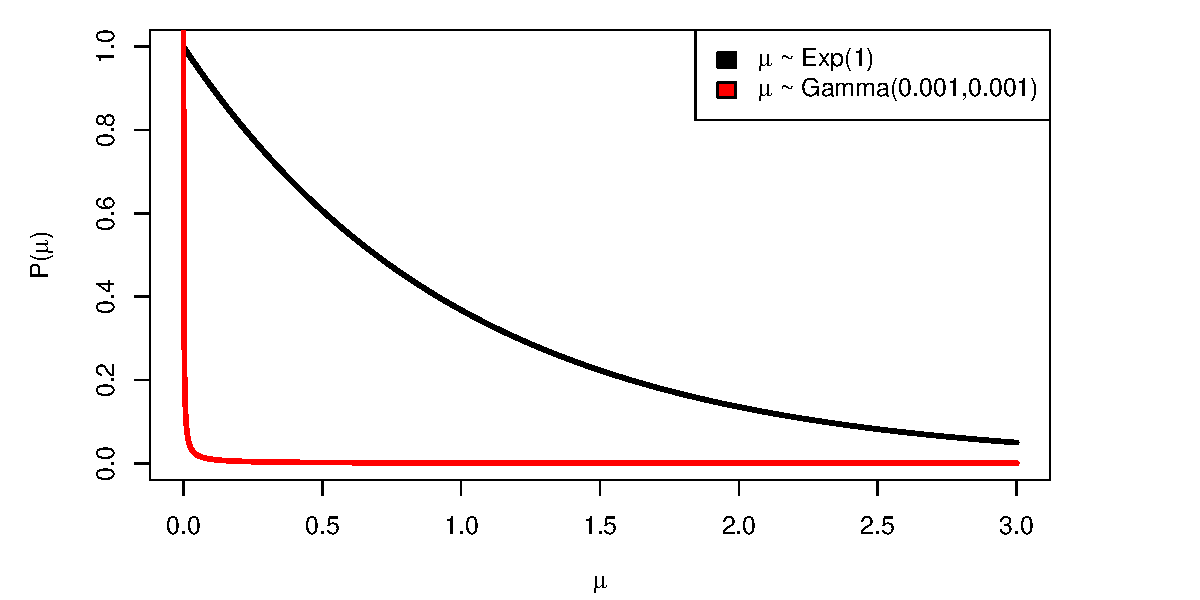
\includegraphics[width=0.7\linewidth,angle=0]{\ResourcePath figures/gamma.pdf}
\caption{Comparison of exponential distribution with $\alpha = 1$ and uninformative gamma distribution with parameters $\alpha=0.001$ and $\beta=0.001$.}
\end{minipage}}
\label{fig:gamma_distribution}
\end{figure}

The second and simplest way we can overcome the informativeness of the prior is to increase the amount of data we collect.
We can do that in our example by increasing the number of arrows we shoot.

\subsection{Exercise 4}

\begin{enumerate}[label=\textnormal{Step \arabic*)},leftmargin=1.5cm]
	\item Increase the true mean arrow distance so that it is significantly larger than $\alpha$. How does this impact your estimate of $\mu$?
	\item Now use an uninformative Gamma$(0.001, 0.001)$ prior for $\mu$. Did your estimate of $\mu$ improve?
	\item Increase the number of arrows shot. How does this change the shape and scale of the posterior distribution?
\end{enumerate}

\bibliographystyle{sysbio}
\bibliography{\GlobalResourcePath refs}


\chapter{Introduction to Markov chain Monte Carlo Algorithms using a Coin-Flip Example}
\def \ResourcePath {RB_MCMC_Binomial_Tutorial/}
\section{Overview}

This very basic tutorial provides an introduction to Bayesian inference and Markov chain Monte Carlo (MCMC) algorithms.
The tutorial explains the fundamental concepts of an MCMC algorithm, such as \emph{moves} and \emph{monitors}, which are ubiquitous in every other tutorial.
After the tutorial you should be somewhat familiar with Bayesian inference (\EG what is a prior distribution, posterior distribution, and likelihood function) and MCMC simulation (\EG what are moves and monitors and why do we need them).

\section{A Coin Flipping (Binomial) Model}

We'll begin our exploration of Bayesian inference with a simple coin-flipping model.
In this model, we imagine flipping a coin $n$ times and count the number of heads, $x$; each flip comes up heads with probability $p$.
This model gives rise to the Binomial probability distribution, with parameters $n$ and $p$:
\begin{align*}
P(x \mid n,p) = {n \choose x}p^x(1-p)^{n-x}
\end{align*}
Simple intuition suggests that, given that we observe $x$ heads in $n$ coin tosses, the maximum-likelihood estimate (MLE) of $p$ is simply $\frac{x}{n}$: if we flip a coin 100 times and observe 70 heads, we assume the probability the coin comes up heads is $\frac{70}{100} = 0.7$.
This is indeed the maximum likelihood estimate!

From Bayes' theorem, the \emph{posterior distribution} of $p$ given $x$, $P(p \mid x)$, is:
\begin{align*}
\overbrace{P(p \mid x)}^{\text{posterior distribution}} = \frac{ \overbrace{P(x \mid p)}^{\text{likelihood}} \times \overbrace{P(p)}^{\text{prior}}}{\underbrace{P(x)}_{\text{marginal likelihood}}}
\end{align*}
The take-home message here is that, if we're interested in doing Bayesian inference for the coin flipping model, we need to specify a \emph{likelihood function} and a \emph{prior distribution} for $p$.
In virtually all practical cases, we cannot compute the posterior distribution directly and instead use numerical procedures, such as a Markov chain Monte Carlo (MCMC) algorithm.
Therefore, we will also have to write an MCMC algorithm that samples parameter values in the frequency of their posterior probability.

We'll use a simple beta distribution as a prior on the parameter of the model, $p$.
The beta distribution has two parameters, $\alpha$ and $\beta$ (Figure~\ref{fig:beta_distribution}).
Different choices for $\alpha$ and $\beta$ represent different prior beliefs.
\begin{figure}[h!]
\centering
\fbox{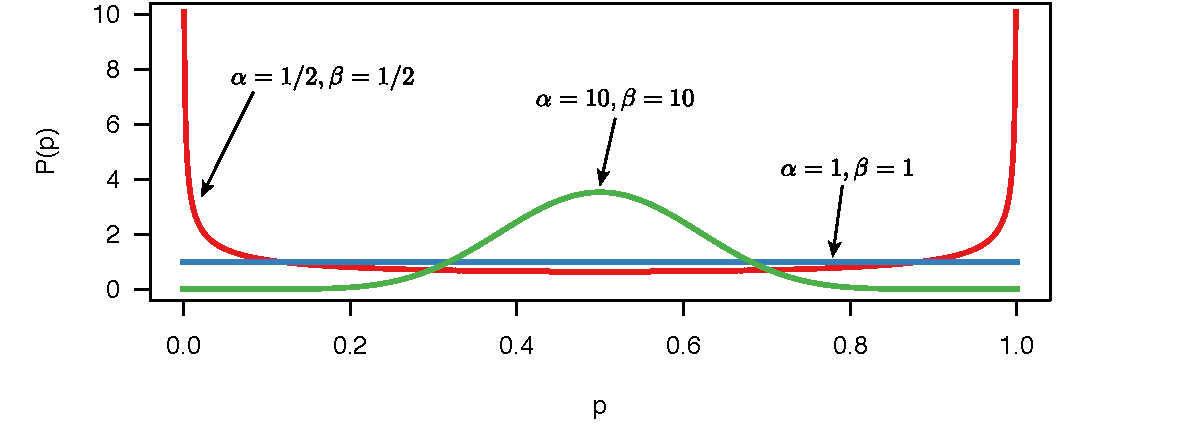
\includegraphics[width=0.7\linewidth,angle=0]{\ResourcePath figures/beta.pdf}}
\label{fig:beta_distribution}
\caption{A beta distribution with two parameters, $\alpha$ and $\beta$. This distribution is used as a prior distribution on the probability parameter $p$ of observing a head. Here we show different curves for the beta distribution when using different parameters.}
\end{figure}


Figure~\ref{fig:binomial_model} shows the graphical model for the binomial model.
This nicely visualizes the dependency structure in the model.
We see that the two parameters $\alpha$ and $\beta$ are drawn in solid squares, representing that these variables are constant.
From these two variables, we see arrows going into the variable $p$.
That simply means that $p$ depends on $\alpha$ and $\beta$.
More specifically, $p$ is a stochastic variable (shown as a solid circle) and drawn from a beta distribution with parameters $\alpha$ and $\beta$.
Then, we have another constant variable, $n$.
Finally, we have the observed data $x$ which is drawn from a Binomial distribution with parameters $p$ and $n$, as can be seen by the arrows going into $x$.
Furthermore, the solid circle of $x$ is shaded which means that the variable has data attached to it.
\begin{figure}[h!]
\centering
\fbox{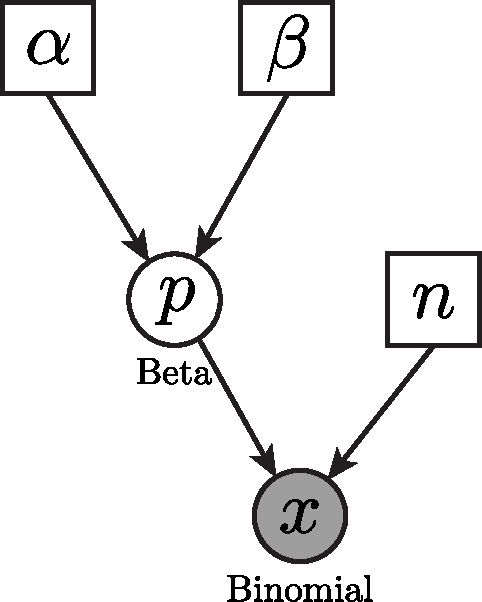
\includegraphics[width=1.8in,angle=0]{\ResourcePath figures/binomial_graphical_model.pdf}}
\label{fig:binomial_model}
\caption{A graphical model for the binomial model.}
\end{figure}



\section{Writing an MCMC from Scratch}

\impmark Make yourself familiar with the example script called \emph{Binomial\_MH\_algorithm.Rev} which shows the code for the following sections. Then, start a new and empty script and follow each step provided in the \colorbox{shadecolor}{blue boxes}.

\subsection{The Metropolis-Hastings Algorithm}
Though \RevBayes implements efficient and easy-to-use Markov chain Monte Carlo algorithms, we'll begin by writing one ourselves to gain a better understanding of the moving parts.
The Metropolis-Hastings MCMC algorithm \citep{Metropolis1953,Hastings1970} proceeds as follows:

\begin{enumerate}
	\item Generate initial values for the parameters of the model (in this case, $p$).
	\item Propose a new value (which we'll call $p^\prime$) for some parameters of the model, (possibly) based on their current values 
	\item Calculate the acceptance probability, $R$, according to:
	\begin{align*}
		R = \text{min}\left\{1, \frac{P(x \mid p^\prime)}{P(x \mid p)} \times \frac{P(p^\prime)}{P(p)} \times \frac{q(p)}{q(p^\prime)} \right\}
	\end{align*}
	\item Generate a uniform random number between 1 and 0. If it is less than $R$, accept the move (set $p = p^\prime$). Otherwise, keep the current value of $p$.
	\item Record the values of the parameters.
	\item Return to step 2 many many times, keeping track of the value of $p$.
\end{enumerate}

\subsection{Reading in the data}
Actually, in this case, we're just going to make up some data on the spot.
Feel free to alter these values to see how they influence the posterior distribution
{\tt \begin{snugshade*}
\begin{lstlisting}    
# Make up some coin flips!
# Feel free to change these numbers
n <- 100 # the number of flips
x <- 63	# the number of heads
\end{lstlisting}
\end{snugshade*}}

\subsection{Initializing the Markov chain}
We have to start the MCMC off with some initial parameter values.
One way to do this is to randomly draw values of the parameters (just $p$, in this case) from the prior distribution.
We'll assume a ``flat'' beta prior distribution; that is, one with parameters $\alpha = 1$ and $\beta = 1$.
{\tt \begin{snugshade*}
\begin{lstlisting}
# Initialize the chain with starting values
alpha <- 1
beta  <- 1
p <- rbeta(n=1,alpha,beta)[1]
\end{lstlisting}
\end{snugshade*}}
\pagebreak
\subsubsection{Likelihood function}
We also need to specify the likelihood function.
We use the binomial probability for the likelihood function. Since the likelihood is defined only for values of $p$ between 0 and 1, we return 0.0 if $p$ is outside this range:
{\tt \begin{snugshade*}
\begin{lstlisting}
# specify the likelihood function
function likelihood(p) {
    if(p < 0 || p > 1)
        return 0

    l = dbinomial(x,p,n,log=false)
    return l
}
\end{lstlisting}
\end{snugshade*}}

\subsubsection{Prior distribution}
Similarly, we need to specify a function for the prior distribution.
Here, we use the beta probability distribution for the prior on $p$:
{\tt \begin{snugshade*}
\begin{lstlisting}    
# specify the prior function
function prior(p) {
    if(p < 0 || p > 1)
        return 0
        
    pp = dbeta(p,alpha,beta,log=false)
    return pp
}
\end{lstlisting}
\end{snugshade*}}


\subsubsection{Monitoring parameter values}
Additionally, we are going to monitor, \IE store, parameter values into a file during the MCMC simulation.
For this file we need to write the column headers:
{\tt \begin{snugshade*}
\begin{lstlisting}
# Prepare a file to log our samples
write("iteration","p","\n",file="binomial_MH.log")
write(0,p,"\n",file="binomial_MH.log",append=TRUE)
\end{lstlisting}
\end{snugshade*}}
(You may have to change the newline characters to \texttt{"$\backslash$r$\backslash$n"} if you're using a Windows operating system.)
We'll also monitor the parameter values to the screen, so let's print the initial values:
{\tt \begin{snugshade*}
\begin{lstlisting}
# Print the initial values to the screen
print("iteration","p")
print(0,p)
\end{lstlisting}
\end{snugshade*}}

\subsection{Writing the MH Algorithm}
At long last, we can write our MCMC algorithm.
First, let us define the frequency how often we print to file (\IE monitor), which is also often called thinning.
If we set the variable \cl{printgen} to 1, then we will store the parameter values every single iteration; if we choose \cl{printgen=10} instead, then only every $10^{th}$ iteration.
{\tt \begin{snugshade*}
\begin{lstlisting}    
printgen = 10
\end{lstlisting}
\end{snugshade*}}
We will repeat this resampling procedure many times (here, 10000), and iterate the MCMC using a \texttt{for} loop:
{\tt \begin{snugshade*}
\begin{lstlisting}    
# Write the MH algorithm
reps = 10000 
for(rep in 1:reps){
\end{lstlisting}
\end{snugshade*}}
(remember to close your \texttt{for} loop at the end).

The first thing we do in the first generation is generate a new value of $p^\prime$ to evaluate.
We'll propose a new value of $p$ from a uniform distribution between 0 and 1.
Note that in this first example we do not condition new parameter values on the current value.
{\tt \begin{snugshade*}
\begin{lstlisting}    
	# Propose a new value of p
	p_prime <- runif(n=1,0.0,1.0)[1]
\end{lstlisting}
\end{snugshade*}}

Next, we compute the proposed likelihood and prior probabilities, as well as the acceptance probability, $R$:
{\tt \begin{snugshade*}
\begin{lstlisting}    
	# Compute the acceptance probability
	R <- ( likelihood(p_prime) / likelihood(p) ) * ( prior(p_prime) / prior(p) )
\end{lstlisting}
\end{snugshade*}}

Then, we accept the proposal with probability $R$ and reject otherwise:
{\tt \begin{snugshade*}
\begin{lstlisting}    
	# Accept or reject the proposal
	u <- runif(1,0,1)[1]
	if(u < R){
		# Accept the proposal
		p <- p_prime
	}
\end{lstlisting}
\end{snugshade*}}

Finally, we store the current value of $p$ in our log file.
Here, we actually check if we want to store the value during this iteration.
{\tt \begin{snugshade*}
\begin{lstlisting}
    if ( (rep % printgen) == 0 ) {
        # Write the samples to a file
        write(rep,p,"\n",file="binomial_MH.log",append=TRUE)
        # Print the samples to the screen
        print(rep,p)
    }
} # end MCMC\end{lstlisting}
\end{snugshade*}}


\subsection{Visualizing the samples of an MCMC simulation}

Below we show an example of the obtained output in \Tracer.
Specifically, Figure~\ref{fig:mcmc_samples} shows the sample trace (left) and the estimated posterior distribution of $p$ (right).
There are other parameters, such as the posterior mean and the 95\% HPD (highest posterior density) interval, that you can obtain from \Tracer.
\begin{figure}[h!]
\centering
\fbox{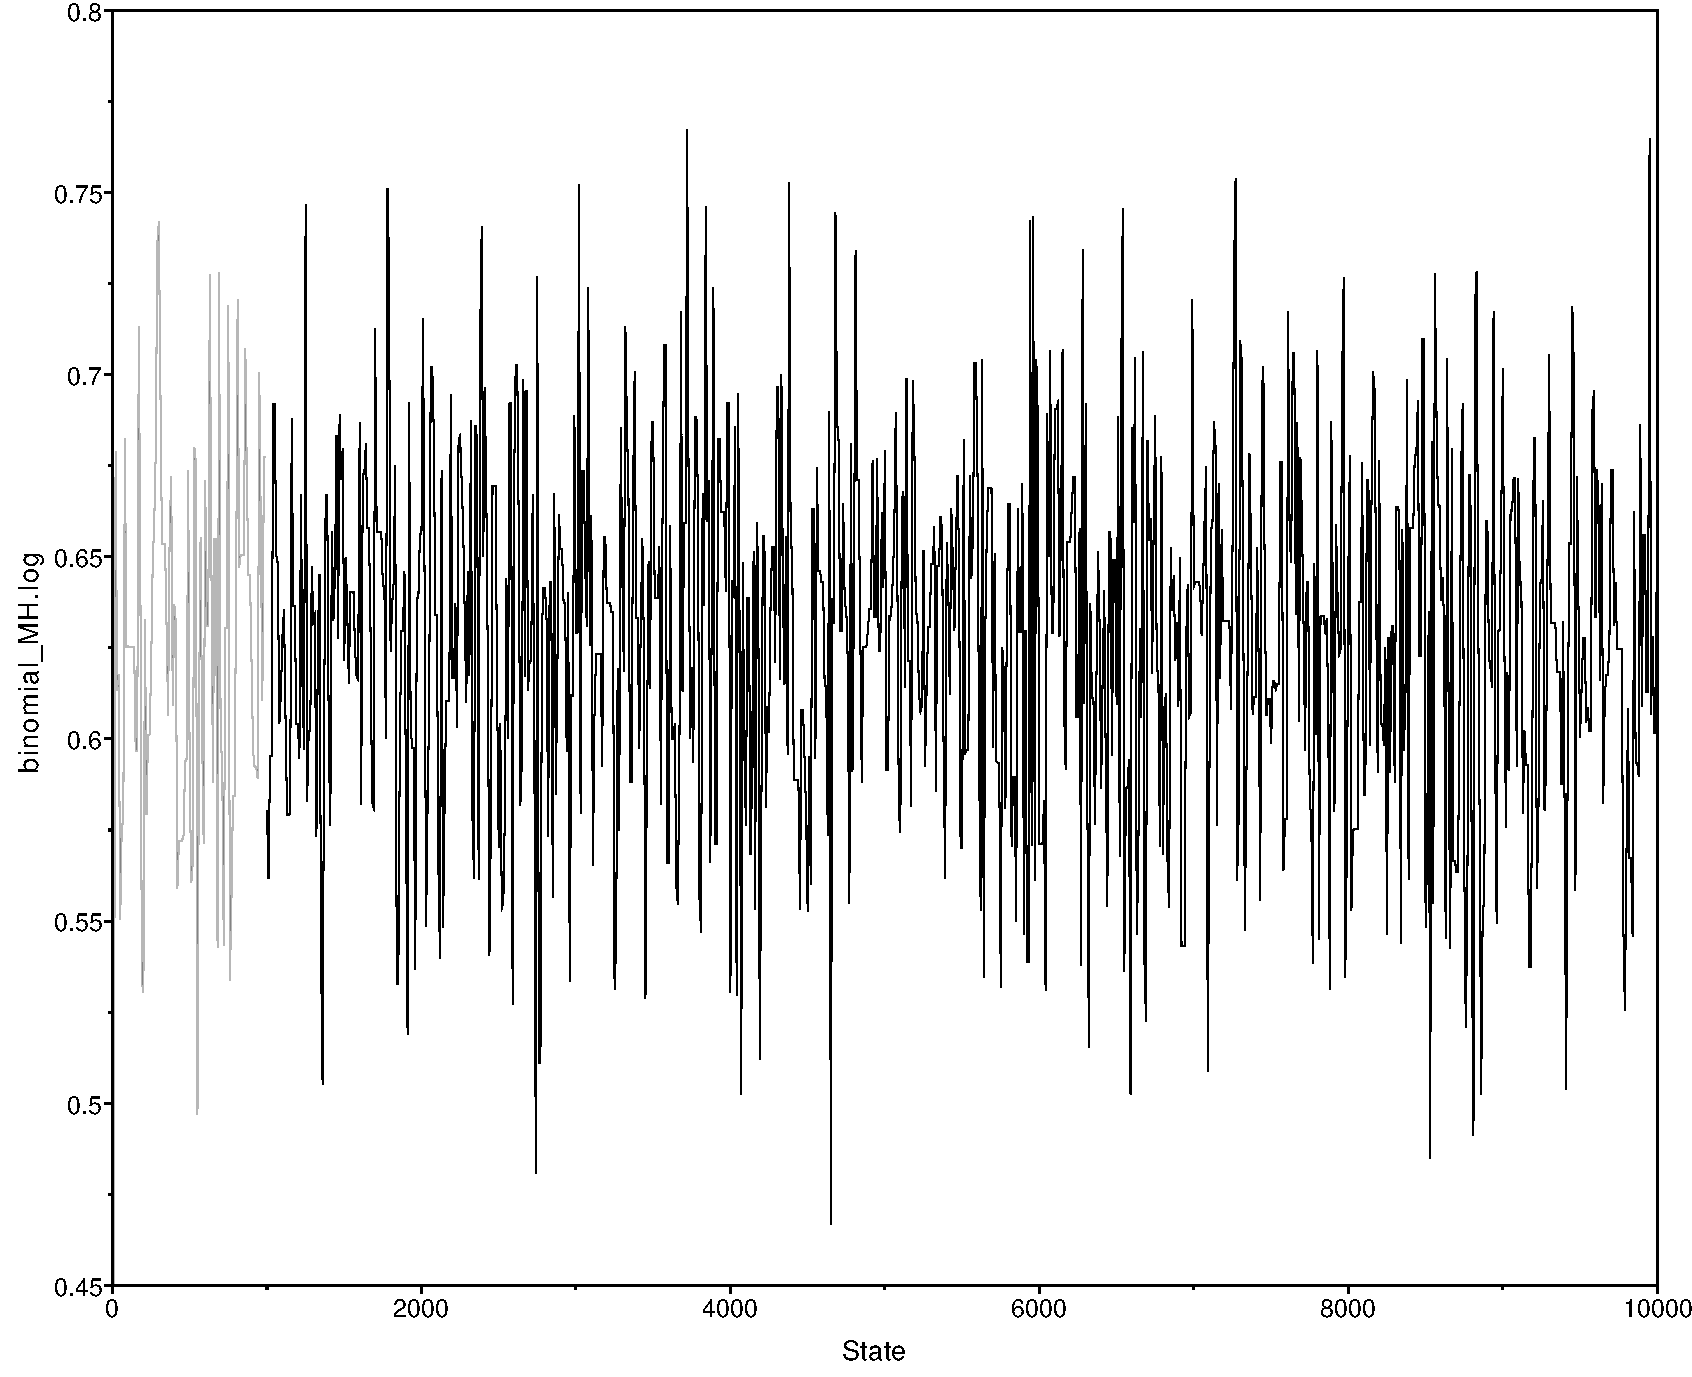
\includegraphics[width=0.45\linewidth,angle=0]{\ResourcePath figures/binomial_MCMC_Trace.pdf}
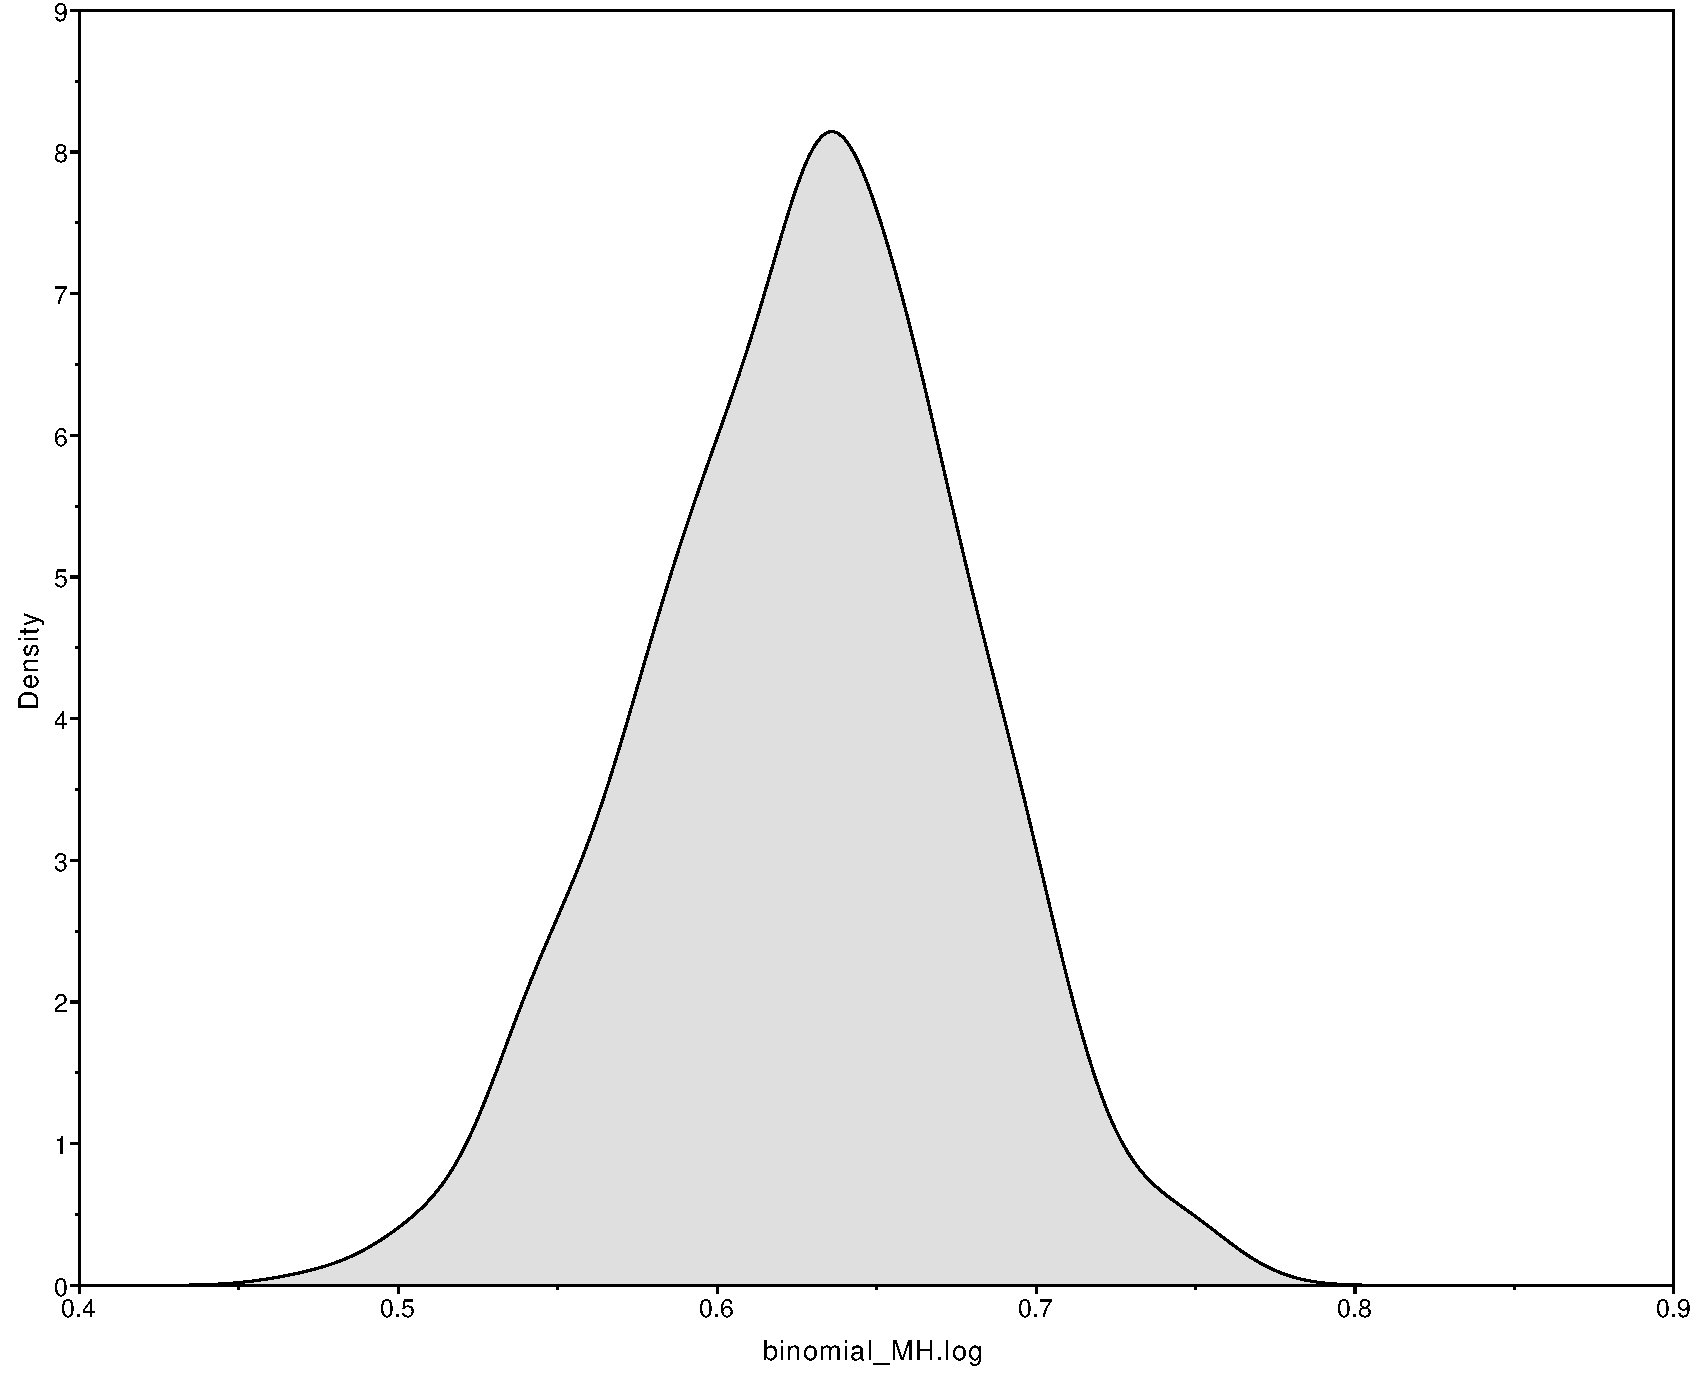
\includegraphics[width=0.45\linewidth,angle=0]{\ResourcePath figures/binomial_MCMC_distribution.pdf}}
\label{fig:mcmc_samples}
\caption{Left: The \emph{Trace} of sample from an MCMC simulation. Right: The approximated posterior probability distribution for $p$.}
\end{figure}

\section{More on Moves: Tuning and weights}

In the previous example we hard coded a single move updating the variable $p$ by drawing a new value from a uniform(0,1) distribution.
There are actually many other ways how to propose new values; some of which are more efficient than others.

First, let us rewrite the MCMC loop so that we use instead a function, which we call \cl{move\_uniform} for simplicity, that performs the move:
{\tt \begin{snugshade*}
\begin{lstlisting}    
for (rep in 1:reps){
    
    # call uniform move
    move_uniform(1)
    
    if ( (rep % printgen) == 0 ) {
        # Write the samples to a file
        write(rep,p,"\n",file="binomial_MH.log",append=TRUE)
    }

} # end MCMC
\end{lstlisting}
\end{snugshade*}}
This loop looks already much cleaner.

\subsection{Uniform move}
Now we need to actually write the \cl{move\_uniform} function.
We mostly just copy the code we had before into a dedicated function
{\tt \begin{snugshade*}
\begin{lstlisting}    
function move_uniform( Natural weight) {

    for (i in 1:weight) {
        # Propose a new value of p
        p_prime <- runif(n=1,0.0,1.0)[1]

        # Compute the acceptance probability
        R <- ( likelihood(p_prime) / likelihood(p) ) * ( prior(p_prime) / prior(p) )
    
        # Accept or reject the proposal
        u <- runif(1,0,1)[1]
        if (u < R){
            # Accept the proposal
            p <- p_prime
        } else {
            # Reject the proposal
            # (we don't have to do anything here)
        }
    }
    
}
\end{lstlisting}
\end{snugshade*}}
There are a few things to consider in the function \cl{move\_uniform}.
First, we do not have a return value because the move simply changes the variable $p$ if the move is accepted.
Second, we expect an argument called \cl{weight} which will tell us how often we want to use this move.
Otherwise, this function does exactly the same what was inside the for loop previously.

(Note that you need to define this function before the for loop in your script).


\subsection{Sliding-window move}
As a second move we will write a sliding-window move.
The sliding-window moves propose an update by drawing a random number from a uniform distribution and then adding this random number to the current value (\IE centered on the previous value).
{\tt \begin{snugshade*}
\begin{lstlisting}    
function move_slide( RealPos delta, Natural weight) {

    for (i in 1:weight) {
        # Propose a new value of p
        p_prime <- p + runiform(n=1,-delta,delta)[1]

        # Compute the acceptance probability
        R <- ( likelihood(p_prime) / likelihood(p) ) * ( prior(p_prime) / prior(p) )
    
        # Accept or reject the proposal
        u <- runif(1,0,1)[1]
        if (u < R) {
            # Accept the proposal
            p <- p_prime
        } else {
            # Reject the proposal
            # (we don't have to do anything here)
        }
    }
    
}
\end{lstlisting}
\end{snugshade*}}
In addition to the weight of the move, this move has another argument, \cl{delta}.
The argument \cl{delta} defines the width of the uniform window from which we draw new values.
Thus, if \cl{delta} is large, then the proposed values are more likely to be very different from the current value of $p$.
Conversely, if \cl{delta} is small, then the proposed values are more likely to be very close to the current value of $p$.

\impmark Experiment with different values for \cl{delta} and check how the effective sample size (ESS) changes.

There is, a priori, no good method for knowing what values of \cl{delta} are most efficient.
However, there are some algorithms implemented in \RevBayes, called \emph{auto-tuning}, that will estimate good values for \cl{delta}.

\subsection{Scaling move}
As a third and final move we will write a scaling move.
The scaling move proposes an update by drawing a random number from a uniform(-0.5,0.5) distribution, exponentiating the random number, and then multiplying this scaling factor by the current value.
An interesting feature of this move is that it is not symmetrical and thus needs a Hastings ratio.
The Hastings ratio is rather trivial in this case, and one only needs to multiply the acceptance rate by the scaling factor.
{\tt \begin{snugshade*}
\begin{lstlisting}    
function move_scale( RealPos lambda, Natural weight) {

    for (i in 1:weight) {
        # Propose a new value of p
        sf <- exp( lambda * ( runif(n=1,0,1)[1] - 0.5 ) )
        p_prime <- p * sf

        # Compute the acceptance probability
        R <- ( likelihood(p_prime) / likelihood(p) ) * ( prior(p_prime) / prior(p) ) * sf
    
        # Accept or reject the proposal
        u <- runif(1,0,1)[1]
        if (u < R){
            # Accept the proposal
            p <- p_prime
        } else {
            # Reject the proposal
            # (we don't have to do anything here)
        }
    }
    
}
\end{lstlisting}
\end{snugshade*}}
As before, this move has a tuning parameter called \emph{lambda}.

\begin{framed}
The sliding-window and scaling moves are very common and popular moves in \RevBayes.
The code examples here are actually showing the exact same equation as implemented internally.
It will be very useful for you to understand these moves.	
\end{framed}

\pagebreak

However, this MCMC algorithm is \emph{very} specific to our binomial model and thus hard to extend (also it's pretty inefficient!).


\section{The Metropolis-Hastings Algorithm with the \emph{Real} \RevBayes}
We'll now specify the exact same model in \Rev using the built-in modeling functionality.
It turns out that the \Rev code to specify the above model is extremely simple and similar to the one we used before.
Again, we start by ``reading in'' (\emph{i.e.}, making up) our data.

{\tt \begin{snugshade*}
\begin{lstlisting}    
# Make up some coin flips!
# Feel free to change these numbers
n <- 100 # the number of flips
x <- 63	# the number of heads
\end{lstlisting}
\end{snugshade*}}

Now we specify our prior model.
{\tt \begin{snugshade*}
\begin{lstlisting}    
# Specify the prior distribution
alpha <- 1
beta  <- 1
p ~ dnBeta(alpha,beta)
\end{lstlisting}
\end{snugshade*}}

One difference between \RevBayes and the MH algorithm that we wrote above is that many MCMC proposals are already built-in, but we have to specify them \emph{before} we run the MCMC.
We usually define (at least) one move per parameter immediately after we specify the prior distribution for that parameter.

{\tt \begin{snugshade*}
\begin{lstlisting}    
# Define a move for our parameter, p
moves[1] = mvSlide(p,delta=0.1,weight=1)
\end{lstlisting}
\end{snugshade*}}

Next, our likelihood model.
{\tt \begin{snugshade*}
\begin{lstlisting}    
# Specify the likelihood model
k ~ dnBinomial(p, n)
k.clamp(x)
\end{lstlisting}
\end{snugshade*}}

We wrap our full Bayesian model into one model object (this is a convenience to keep the entire model in a single object, and is more useful when we have very large models):
{\tt \begin{snugshade*}
\begin{lstlisting}    
# Construct the full model
my_model = model(p)
\end{lstlisting}
\end{snugshade*}}

We use ``monitors'' to keep track of parameters throughout the MCMC.
The two kinds of monitors we use here are the \texttt{mnModel}, which writes parameters to a specified file, and the \texttt{mnScreen}, which simply outputs some parts of the model to screen (as a sort of progress bar).
{\tt \begin{snugshade*}
\begin{lstlisting}    
# Make the monitors to keep track of the MCMC
monitors[1] = mnModel(filename="binomial_MCMC.log", printgen=10, separator = TAB)
monitors[2] = mnScreen(printgen=100, p)
\end{lstlisting}
\end{snugshade*}}

Finally, we assemble the analysis object (which contains the model, the monitors, and the moves) and execute the run using the \texttt{.run} command:
{\tt \begin{snugshade*}
\begin{lstlisting}    
# Make the analysis object
analysis = mcmc(my_model, monitors, moves)

# Run the MCMC
analysis.run(100000)

# Show how the moves performed
analysis.operatorSummary()
\end{lstlisting}
\end{snugshade*}}
\impmark Open the resulting \texttt{binomial\_MCMC.log} file in \texttt{Tracer}.
Do the posterior distributions for the parameter $p$ look the same as the ones we got from our first analysis?

Hopefully, you'll note that this \Rev model is substantially simpler and easier to read than the MH algorithm script we began with.
Perhaps more importantly, this \Rev analysis is \emph{orders of magnitude} faster than our own script, because it makes use of extremely efficient probability calculations built-in to \RevBayes (rather than the ones we hacked together in our own algorithm).


\bibliographystyle{sysbio}
\bibliography{\GlobalResourcePath refs}






\section{Exercises for the MCMC Tutorial}


\subsection{Exercise 1: Performing your first simple MCMC simulation}

\begin{enumerate}[label=\textnormal{\arabic*)}]
	\item Look into the \emph{Binomial\_MH\_algorithm.Rev} script and make yourself familiar with it. All the commands should be explained in the text of the tutorial. 
	\item Execute the script \emph{Binomial\_MH\_algorithm.Rev}).
	\item The \texttt{.log} file will contain samples from the posterior distribution of the model! Open the file in \Tracer to learn about various features of the posterior distribution, for example: the posterior mean or the 95\% credible interval.
	\item Save the MCMC trace plot and posterior distribution into a PDF file and upload the files. Write here the name of your file:\medskip\\
\TextField[name=mcmc_trace,backgroundcolor=TextFieldBackgroundColor,color=TextFieldTextColor,bordercolor=TextFieldBoxColor,height=1cm,width=\TextFieldWidth,multiline=true]{}
\end{enumerate}

\subsection{Exercise 2: Different MCMC strategies (moves)}

\begin{enumerate}[label=\textnormal{\arabic*)}]
	\item Now look into the script called \emph{Binomial\_MH\_algorithm\_moves.Rev} which shows the 3 different types of moves described in this tutorial.
	\item Run the script to estimate the posterior distribution of $p$ again.
	\item Look at the output in \Tracer.
%	\item Are the distributions, mean and credible interval the same?
	\item Use only a single move and set \cl{printgen=1}. Which move has the best ESS? Enter the ESS values for the different moves here:\medskip\\
\TextField[name=mcmc_ESS,,backgroundcolor=TextFieldBackgroundColor,color=TextFieldTextColor,bordercolor=TextFieldBoxColor,height=2cm,width=\TextFieldWidth,multiline=true]{}
	\item How does the ESS change if you use a \cl{delta=10} for the sliding-window move?\medskip\\
\TextField[name=mcmc_ESS_delta,,backgroundcolor=TextFieldBackgroundColor,color=TextFieldTextColor,bordercolor=TextFieldBoxColor,height=1cm,width=\TextFieldWidth,multiline=true]{}
	\item Add to each move a counter variable that counts how often the move was accepted. For example:
{\tt \begin{snugshade*}
\begin{lstlisting}    
        if (u < R){
            # Accept the proposal
            p <- p_prime
            ++num_sliding_move_accepted
        } \end{lstlisting}
\end{snugshade*}}
	\item Have a look at how the acceptance rate changes for different values of the tuning parameters.\medskip\\
\TextField[name=mcmc_acceptance,,backgroundcolor=TextFieldBackgroundColor,color=TextFieldTextColor,bordercolor=TextFieldBoxColor,height=2cm,width=\TextFieldWidth,multiline=true]{}
\end{enumerate}

\subsection{Exercise 3: MCMC in \RevBayes}

\begin{enumerate}[label=\textnormal{\arabic*)}]
	\item Run the built-in MCMC (\emph{Binomial\_MCMC.Rev}) and compare the results to your own MCMC. Are the posterior estimates the same? Are the ESS values similar? Which script was the fastest?\medskip\\
\TextField[name=mcmc_builtin,,backgroundcolor=TextFieldBackgroundColor,color=TextFieldTextColor,bordercolor=TextFieldBoxColor,height=2cm,width=\TextFieldWidth,multiline=true]{}
	\item Next, add a second move \cl{moves[2] = mvScale(p,lambda=0.1,tune=true,weight=1.0)} just after the first one.
	\item Run the analysis again and upload your trace file. Write here the name of your file:\medskip\\
\TextField[name=mcmc_trace_builtin,,backgroundcolor=TextFieldBackgroundColor,color=TextFieldTextColor,bordercolor=TextFieldBoxColor,height=1cm,width=\TextFieldWidth,multiline=true]{}
	\item Finally, run a pre-burnin using \cl{analysis.burnin(generations=10000,tuningInterval=200)} just before you call \cl{analysis.run(100000)}. This will auto-tune the tuning parameters (\EG \cl{delta} and \cl{lambda}) so that the acceptance ratio is between 0.4 and 0.5.
	\item What are the tuned values for \cl{delta} and \cl{lambda}? Did the auto-tuning increase the ESS?\medskip\\
\TextField[name=mcmc_autotunig,backgroundcolor=,backgroundcolor=TextFieldBackgroundColor,color=TextFieldTextColor,bordercolor=TextFieldBoxColor,height=2cm,width=\TextFieldWidth,multiline=true]{}
\end{enumerate}


\subsection{Exercise 4: Approximating the posterior distribution}

Modify the script \emph{Binomial\_MCMC.Rev}. Assume you flipped a coin 100 times and got 34 heads. Run the MCMC for 100,000 generations, printing every 100 samples to the file. 

\begin{enumerate}[label=\textnormal{\arabic*)}]
	\item What is the posterior mean estimate of p? The 95\% credible interval?\medskip\\
\TextField[name=mcmc_posterior_estimates,backgroundcolor=TextFieldBackgroundColor,color=TextFieldTextColor,bordercolor=TextFieldBoxColor,height=2cm,width=\TextFieldWidth,multiline=true]{}
	\item Pretend you flipped the coin 900 more times, for a total of 1000 flips. Among those 1000 flips, you observed 340 heads (change your script accordingly!). What is your posterior mean estimate of p now? How has the 95\% credible interval changed? Provide an intuitive explanation for this change.\medskip\\
\TextField[name=mcmc_posterior_estimates_large,,backgroundcolor=TextFieldBackgroundColor,color=TextFieldTextColor,bordercolor=TextFieldBoxColor,height=2cm,width=\TextFieldWidth,multiline=true]{}
\end{enumerate}


\subsection{Exercise 5: Exploring prior sensitivity and MCMC settings}
Play around with various parts of the model to develop on intuition for both the Bayesian model and the MCMC algorithm.
For example, how does the posterior distribution change as you increase the number of coin flips (say, increase both the number of flips and the number of heads by an order of magnitude)?
How does the estimated posterior distribution change if you change the prior model parameters, $\alpha$ and $\beta$ (\IE is the model prior sensitive)?
Does the prior sensitivity depend on the sample size?
Are the posterior estimates sensitive to the length of the MCMC?
Do you think this MCMC has been run sufficiently long, or should you run it longer? Try to answer some of these questions and explain your finding here:\\
\forceindent\TextField[name=mcmc_exploration,backgroundcolor=TextFieldBackgroundColor,color=TextFieldTextColor,bordercolor=TextFieldBoxColor,height=5cm,width=\TextFieldWidth,multiline=true]{}



%\chapter{More on Markov chain Monte Carlo Algorithms}
%\def \ResourcePath {RB_MCMC_Tutorial/}
%\include{RB_MCMC_Tutorial/RB_MCMC_Tutorial_content}

\part{Model Selection, Model Averaging, and Model Testing}

\chapter{Model Selection and Bayes Factors}
\def \ResourcePath {RB_BayesFactor_Tutorial/}
\section{Overview}

This tutorial provides the third protocol from our recent publication \citep{Hoehna2017a}.
The first protocol is described in the \href{https://github.com/revbayes/revbayes_tutorial/raw/master/tutorial_TeX/RB_CTMC_Tutorial/RB_CTMC_Tutorial.pdf}{Substitution model tutorial} and the second protocol is described in the \href{https://github.com/revbayes/revbayes_tutorial/raw/master/tutorial_TeX/RB_Partition_Tutorial/RB_Partition_Tutorial.pdf}{Partitioned data analysis tutorial}.

This tutorial demonstrates some general principles of Bayesian model comparison, which is based on estimating the marginal likelihood of competing models and then comparing their relative fit to the data using Bayes factors.
We consider the specific case of calculating Bayes factors to select among different substitution models.

\subsection{Requirements}
We assume that you have read and hopefully completed the following tutorials:
\begin{itemize}
\item \href{https://github.com/revbayes/revbayes_tutorial/raw/master/tutorial_TeX/RB_Getting_Started/RB_Getting_Started.pdf}{Getting started}
\item \href{https://github.com/revbayes/revbayes_tutorial/raw/master/tutorial_TeX/RB_Intro_Tutorial/RB_Intro_Tutorial.pdf}{\Rev basics}
\item \href{https://github.com/revbayes/revbayes_tutorial/raw/master/tutorial_TeX/RB_Rev_Tutorial/RB_Rev_Tutorial.pdf}{\Rev syntax}
\item \href{https://github.com/revbayes/revbayes_tutorial/raw/master/tutorial_TeX/RB_CTMC_Tutorial/RB_CTMC_Tutorial.pdf}{Substitution models}
\end{itemize}
Note that the \href{https://github.com/revbayes/revbayes_tutorial/raw/master/tutorial_TeX/RB_Intro_Tutorial/RB_Intro_Tutorial.pdf}{\Rev basics tutorial} introduces the basic syntax of \Rev but does not cover any phylogenetic models.
We tried to keep this tutorial very basic and introduce all the language concepts and theory on the way.
You may only need the \href{https://github.com/revbayes/revbayes_tutorial/raw/master/tutorial_TeX/RB_Rev_Tutorial/RB_Rev_Tutorial.pdf}{\Rev syntax tutorial} for a more in-depth discussion of concepts in \Rev.



%%%%%%%%
%%   Data   %%
%%%%%%%%
\section{Data and files}

We provide the data file that we will use in this tutorial.
Of course, you may want to use your own dataset instead.
In the \cl{data} folder, you will find the following file:
\begin{itemize}
\item
\cl{primates\_and\_galeopterus\_cytb.nex}: Alignment of the \textit{cytochrome b} subunit from 23 primates representing 14 of the 16 families (\textit{Indriidae} and \textit{Callitrichidae} are missing).
\end{itemize}



\section{Introduction}

For most sequence alignments, several (possibly many) substitution models of varying complexity are plausible \emph{a priori}.
We therefore need a way to objectively identify the model that balances estimation bias and inflated error variance associated with under- and over-parameterized models, respectively.
Increasingly, model selection is based on \emph{Bayes factors} \citep[\EG][]{Suchard2001,Lartillot2006,Xie2011,Baele2012,Baele2013}, which involves first calculating the marginal likelihood of each candidate model and then comparing the ratio of the marginal likelihoods for the set of candidate models.

 
Given two models, $M_0$ and $M_1$, the Bayes-factor comparison assessing the relative fit of each model to the data, $BF(M_0,M_1)$, is:
$$BF(M_0,M_1) = \frac{\mbox{posterior odds}}{\mbox{prior odds}}.$$
The posterior odds is the posterior probability of $M_0$ given the data, $\mathbf X$, divided by the posterior odds of $M_1$ given the data:
$$\mbox{posterior odds} = \frac{\mathbb{P}(M_0 \mid \mathbf X)}{\mathbb{P}(M_1 \mid \mathbf X)},$$
and the prior odds is the prior probability of $M_0$ divided by the prior probability of $M_1$:
$$\mbox{prior odds} = \frac{\mathbb{P}(M_0)}{\mathbb{P}(M_1)}.$$
Thus, the Bayes factor measures the degree to which the data alter our belief regarding the support for $M_0$ relative to $M_1$ \citep{Lavine1999}:
\begin{align}\label{BFeq1}
BF(M_0,M_1) = \frac{\mathbb{P}(M_0 \mid \mathbf X, \theta_0)}{\mathbb{P}(M_1 \mid \mathbf X, \theta_1)} \div \frac{\mathbb{P}(M_0)}{\mathbb{P}(M_1)}. 
\end{align}
Note that interpreting Bayes factors involves some subjectivity.
That is, it is up to \textsl{you} to decide the degree of your belief in $M_0$ relative to $M_1$. 
Despite the absence of an absolutely objective model-selection threshold, we can refer to the scale \citep[outlined by][]{Jeffreys1961} that provides a ``rule-of-thumb'' for interpreting these measures (Table \ref{bftable}).
\begin{table}[h]
\centering
\caption{\small The scale for interpreting Bayes factors by Harold \citet{Jeffreys1961}.} 
\label{bftable}
\begin{tabular}{l c c c}
\hline
\multicolumn{1}{r}{{Strength of evidence}} & \multicolumn{1}{l}{\textbf{$BF(M_0, M_1)$}} & \multicolumn{1}{l}{\textbf{log($BF(M_0, M_1)$)}} &  \multicolumn{1}{l}{\textbf{$\text{log}_{10}$($BF(M_0, M_1)$)}}\\ 
\hline
Negative (supports $M_1$) & $<1$ & $<0$ & $<0$\\
Barely worth mentioning & $1$ to $3.2$ & $0$ to $1.16$ & $0$ to $0.5$\\
Substantial & $3.2$ to $10$ & $1.16$ to $2.3$ & $0.5$ to $1$ \\
Strong & $10$ to $100$ & $2.3$ to $4.6$ & $1$ to $2$ \\
Decisive& $>100$ & $>4.6$ & $>2$ \\
\hline
\multicolumn{3}{l}{{\scriptsize{For a detailed description of Bayes factors see \citet{Kass1995}}}} 
\end{tabular}
\end{table}


Unfortunately, it is generally not possible to directly calculate the posterior odds to prior odds ratios.
However, we can further define the posterior odds ratio as:
\begin{align*}
\frac{\mathbb{P}(M_0 \mid \mathbf X)}{\mathbb{P}(M_1 \mid \mathbf X)} = \frac{\mathbb{P}(M_0)}{\mathbb{P}(M_1)} \frac{\mathbb{P}(\mathbf X \mid M_0)}{\mathbb{P}(\mathbf X \mid M_1)},
\end{align*}
where $\mathbb{P}(\mathbf X \mid M_i)$ is the \textit{marginal likelihood} of the data (this may be familiar to you as the denominator of Bayes Theorem, which is variously referred to as the \textit{model evidence} or \textit{integrated likelihood}).
Formally, the marginal likelihood is the probability of the observed data ($\mathbf X$) under a given model ($M_i$) that is averaged over all possible values of the parameters of the model ($\theta_i$) with respect to the prior density on $\theta_i$
\begin{align}\label{margeLike}
\mathbb{P}(\mathbf X \mid M_i) = \int \mathbb{P}(\mathbf X \mid \theta_i) \mathbb{P}(\theta_i)dt.
\end{align}
This makes it clear that more complex (parameter-rich) models are penalized by virtue of the associated prior: each additional parameter entails integration of the likelihood over the corresponding prior density.  
If you refer back to equation \ref{BFeq1}, you can see that, with very little algebra, the ratio of marginal likelihoods is equal to the Bayes factor:
\begin{align}\label{bfFormula}
BF(M_0,M_1) = \frac{\mathbb{P}(\mathbf X \mid M_0)}{\mathbb{P}(\mathbf X \mid M_1)} = \frac{\mathbb{P}(M_0 \mid \mathbf X, \theta_0)}{\mathbb{P}(M_1 \mid \mathbf X, \theta_1)} \div \frac{\mathbb{P}(M_0)}{\mathbb{P}(M_1)}. 
\end{align}
Therefore, we can perform a Bayes factor comparison of two models by calculating the marginal likelihood for each one. % Simple as pie, right?
Alas, exact solutions for calculating marginal likelihoods are not known for phylogenetic models (see equation \ref{margeLike}), thus we must resort to numerical integration methods to estimate or approximate these values. 
In this exercise, we will estimate the marginal likelihood for each partition scheme
using both the stepping-stone \citep{Xie2011,Fan2011} and path sampling estimators \citep{Lartillot2006, Baele2012}. 



\bigskip
\subsection{Substitution Models} 

The models we use here are equivalent to the models described in the previous exercise on substitution models (continuous time Markov models).
To specify the model please consult the previous exercise. Specifically, you will need to specify the following substitution models:
\begin{itemize}
\item Jukes-Cantor (JC) substitution model \citep{Jukes1969}
\item Hasegawa-Kishino-Yano (HKY) substitution model \citep{Hasegawa1985}
\item General-Time-Reversible (GTR) substitution model \citep{Tavare1986}
\item Gamma (+G) model for among-site rate variation \citep{Yang1994a}
\item Invariable-sites (+I) model \citep{Hasegawa1985}
\end{itemize}


\bigskip
\subsection{Estimating the Marginal Likelihood}

We will estimate the marginal likelihood of a given model using a `stepping-stone' (or `path-sampling') algorithm.
These algorithms are similar to the familiar MCMC algorithms, which are intended to sample from (and estimate) the joint posterior probability of the model parameters.
Stepping-stone algorithms are like a series of MCMC simulations that iteratively sample from a specified number of distributions that are discrete steps between the posterior and the prior probability distributions.
The basic idea is to estimate the probability of the data for all points between the posterior and the prior---effectively summing the probability of the data over the prior probability of the parameters to estimate the marginal likelihood. 
Technically, the steps correspond to a series of \cl{powerPosteriors()}, where the likelihood is iteratively raised to a series of numbers between 1 and 0 (Figure~\ref{fig:ss}).
When the likelihood is raised to the power of 1 (typically the first stepping stone), samples are drawn from the (untransformed) posterior.
By contrast, when the likelihood is raised to the power of 0 (typically the last stepping stone), samples are drawn from the prior.
To perform a stepping-stone simulation, we need to specify (1) the number of stepping stones (power posteriors) that we will use to traverse the path between the posterior and the prior (\EG we specify 50 or 100 stones), (2) the spacing of the stones between the posterior and prior (\EG we may specify that the stones are distributed according to a beta distribution), (3) the number of samples (and their thinning) to be drawn from each stepping stone, and (4) the direction we will take (\IE from the posterior to the prior or vice versa).



\begin{figure}[h!]
\centering
\fbox{\includegraphics[width=\textwidth,angle=0]{\ResourcePath figures/ss.pdf}}
\caption{\small Estimating marginal likelihoods using stepping-stone simulation. 
Estimating the marginal likelihood involves integrating the likelihood of the data over the entire prior probability density for the model parameters.
MCMC algorithms target the posterior probability density, which is typically concentrated in a small region of the prior probability density (A).
Accordingly, standard MCMC simulation cannot provide unbiased estimates of the marginal likelihood because it will typically fail to explore most of the prior density.
(B) Stepping-stone algorithms estimate the marginal likelihood by means of a series of MCMC-like simulations, where the likelihood is iteratively raised to a series of powers, effectively forcing the simulation to more fully explore the prior density of the model parameters.
Here, six uniformly spaced stones span the posterior, where the power posterior is $\beta=6/6=1$, to the prior, where the power posterior is $\beta=0/6=0$.}
\label{fig:ss}
\end{figure}


This method computes a vector of powers from a beta distribution, then executes an MCMC run for each power step while raising the likelihood to that power. In this implementation, the vector of powers starts with 1, sampling the likelihood close to the posterior and incrementally sampling closer and closer to the prior as the power decreases. 

Just to be safe, it is better to clear the workspace (if you did not just restart \RevBayes):
{\tt \begin{snugshade*}
\begin{lstlisting}
clear()
\end{lstlisting}
\end{snugshade*}}

Now set up the model as in the previous exercise. You should start with the simple Jukes-Cantor substitution model. 
Setting up the model requires:
\begin{enumerate}
\item Loading the data and retrieving useful variables about it (\EG number of sequences and taxon names).
\item Specifying the instantaneous-rate matrix of the substitution model.
\item Specifying the tree model including branch-length variables.
\item Creating a random variable for the sequences that evolved under the \cl{PhyloCTMC}.
\item Clamping the data.
\item Creating a model object.
\item Specifying the moves for parameter updates.
\end{enumerate}

The following procedure for estimating marginal likelihoods is valid for any model in \RevBayes.
You will need to repeat this later for other models.
First, we create the variable containing the power-posterior analysis. 
This requires that we provide a model and vector of moves, as well as an output file name. 
The \cl{cats} argument sets the number of stepping stones.
{\tt \begin{snugshade*}
\begin{lstlisting}
pow_p = powerPosterior(mymodel, moves, monitors, "output/model1.out", cats=50) 
\end{lstlisting}
\end{snugshade*}}

We can start the power-posterior analysis by first burning in the chain and and discarding the first 10000 states.  
This will help ensure that analysis starts from a region of high posterior probability, rather than from some random point.
{\tt \begin{snugshade*}
\begin{lstlisting}
pow_p.burnin(generations=10000,tuningInterval=1000)
\end{lstlisting}
\end{snugshade*}}

Now execute the run with the \cl{.run()} function:
{\tt \begin{snugshade*}
\begin{lstlisting}
pow_p.run(generations=1000)  
\end{lstlisting}
\end{snugshade*}}

Once the power posteriors have been saved to file, create a stepping stone sampler. 
This function can read any file of power posteriors and compute the marginal likelihood using stepping-stone sampling. 
{\tt \small \begin{snugshade*}
\begin{lstlisting}
ss = steppingStoneSampler(file="output/model1.out", powerColumnName="power", likelihoodColumnName="likelihood")
\end{lstlisting}
\end{snugshade*}}

These commands will execute a stepping-stone simulation with 50 stepping stones, sampling 1000 states from each step. 
Compute the marginal likelihood under stepping-stone sampling using the member function \cl{marginal()} of the \cl{ss} variable and record the value in Table \ref{tab:ml_cytb}.
{\tt \begin{snugshade*}
\begin{lstlisting}
ss.marginal() 
\end{lstlisting}
\end{snugshade*}}

Path sampling is an alternative to stepping-stone sampling and also takes the same power posteriors as input. 
{\tt \small \begin{snugshade*}
\begin{lstlisting}
ps = pathSampler(file="output/model1.out", powerColumnName="power", likelihoodColumnName="likelihood")
\end{lstlisting}
\end{snugshade*}}

Compute the marginal likelihood under stepping-stone sampling using the member function \cl{marginal()} of the \cl{ps} variable and record the value in Table \ref{tab:ml_cytb}.
{\tt \begin{snugshade*}
\begin{lstlisting}
ps.marginal() 
\end{lstlisting}
\end{snugshade*}}

\noindent \\ \impmark As an example we provide the file \textbf{RevBayes\_scripts/marginalLikelihood\_JukesCantor.Rev}.

\begin{framed}
We have kept this description of how to use stepping-stone-sampling and path-sampling very generic and did not provide the information about the model here.
Our main motivation is to show that the marginal likelihood estimation algorithms are independent of the model.
Thus, you can apply these algorithms to any	model, \EG relaxed clock models and birth-death models, as well.
\end{framed}



\subsection{Exercises}

\begin{itemize}
\item Compute the marginal likelihoods of the \textit{cytb} alignment for the following substitution models:
\begin{itemize}
\item Jukes-Cantor (JC) substitution model
\item Hasegawa-Kishino-Yano (HKY) substitution model
\item General-Time-Reversible (GTR) substitution model
\item GTR with gamma distributed-rate model (GTR+G)
\item GTR with invariable-sites model  (GTR+I)
\item GTR+I+G model
\end{itemize}
\item Enter the marginal likelihood estimate for each model in the corresponding cell of Table~\ref{tab:ml_cytb}.
%\item Repeat the above marginal likelihood analyses for the \textit{mt-COX2 gene} and enter results in Table~\ref{tab:ml_cox2}.
\item Which is the best fitting substitution model?
\end{itemize}

\begin{Form}
\begin{table}[h]
\centering
\caption{\small Estimated marginal likelihoods for different substitution models for the cytb alignment$^*$.}
\begin{tabular}{l c c c c}
\hline
\multicolumn{1}{l}{\textbf{ }} &\multicolumn{1}{r}{\textbf{ }} & \multicolumn{3}{c}{\textbf{Marginal lnL estimates}} \\ 
\cline{3-5}
\multicolumn{1}{l}{\textbf{Substitution Model}} & \multicolumn{1}{r}{\hspace{3mm}} & \multicolumn{1}{c}{\textit{Stepping-stone}} & \multicolumn{1}{r}{\hspace{3mm}} & \multicolumn{1}{c}{\textit{Path sampling}} \\ 
\hline
JC ($M_1$) & \hspace{15mm} & \TextField[name=gene1_m11,backgroundcolor={.85 .85 .85},color={1 0 0},height=4ex]{}  & \hspace{15mm} & \TextField[name=gene1_m12,backgroundcolor={.85 .85 .85},color={0 0 1},height=4ex]{} \\
\hline
HKY ($M_2$) & \hspace{3mm} &\TextField[name=gene1_m21,backgroundcolor={.85 .85 .85},color={1 0 0},height=4ex]{}   & \hspace{3mm} & \TextField[name=gene1_m22,backgroundcolor={.85 .85 .85},color={0 0 1},height=4ex]{} \\
\hline
GTR ($M_3$) & \hspace{3mm} &\TextField[name=gene1_m31,backgroundcolor={.85 .85 .85},color={1 0 0},height=4ex]{}   & \hspace{3mm} & \TextField[name=gene1_m32,backgroundcolor={.85 .85 .85},color={0 0 1},height=4ex]{} \\
\hline
GTR+$\Gamma$ ($M_4$) & \hspace{3mm} & \TextField[name=gene1_m41,backgroundcolor={.85 .85 .85},color={1 0 0},height=4ex]{} & \hspace{3mm} & \TextField[name=gene1_m42,backgroundcolor={.85 .85 .85},color={0 0 1},height=4ex]{} \\
\hline
GTR+I ($M_5$) & \hspace{3mm} & \TextField[name=gene1_m51,backgroundcolor={.85 .85 .85},color={1 0 0},height=4ex]{} & \hspace{3mm} & \TextField[name=gene1_m52,backgroundcolor={.85 .85 .85},color={0 0 1},height=4ex]{} \\
\hline
GTR+$\Gamma$+I ($M_6$) & \hspace{3mm} & \TextField[name=gene1_m61,backgroundcolor={.85 .85 .85},color={1 0 0},height=4ex]{} & \hspace{3mm} & \TextField[name=gene1_m62,backgroundcolor={.85 .85 .85},color={0 0 1},height=4ex]{} \\
\hline
{\footnotesize{$^*$you can edit this table}}\\
\end{tabular}
\label{tab:ml_cytb}
\end{table}
\end{Form}



\FloatBarrier
\section{Computing Bayes Factors and Model Selection}

Now that we have estimates of the marginal likelihood for each of our the candidate substitution models, we can evaluate their relative fit to the datasets using Bayes factors.
Phylogenetic programs log-transform the likelihood values to avoid \href{http://en.wikipedia.org/wiki/Arithmetic_underflow}{underflow}: multiplying likelihoods (numbers $< 1$) generates numbers that are too small to be held in computer memory.
Accordingly, we need to use a different form of equation \ref{bfFormula} to calculate the ln-Bayes factor (we will denote this value $\mathcal{K}$):
\begin{align}\label{LNbfFormula}
\mathcal{K}=\ln[BF(M_0,M_1)] = \ln[\mathbb{P}(\mathbf X \mid M_0)]-\ln[\mathbb{P}(\mathbf X \mid M_1)],
\end{align}
where $\ln[\mathbb{P}(\mathbf X \mid M_0)]$ is the \textit{marginal lnL} estimate for model $M_0$. 
The value resulting from equation \ref{LNbfFormula} can be converted to a raw Bayes factor by simply taking the exponent of $\cal{K}$
\begin{align}\label{LNbfFormula2}
BF(M_0,M_1) = e^{\cal{K}}.
\end{align}
Alternatively, you can directly interpret the strength of evidence in favor of $M_0$ in log space by comparing the values of $\cal{K}$ to the appropriate scale (Table \ref{bftable}, second column).
In this case, we evaluate $\cal{K}$ in favor of model $M_0$ against model $M_1$ so that:
\begin{center}
\begin{tabular}{l}
if $\mathcal{K} > 1$, model $M_0$ is preferred\\
if $\mathcal{K} < -1$, model $M_1$ is preferred.
\end{tabular}
\end{center}
Thus, values of $\mathcal{K}$ around 0 indicate that there is no preference for either model. 

Using the values you entered in Table \ref{tab:ml_cytb} and equation \ref{LNbfFormula}, calculate the ln-Bayes factors (using $\mathcal{K}$) for each model comparison. 
Enter your answers in Table \ref{bfTable2} using the stepping-stone and the path-sampling estimates of the marginal log-likelihoods. 

\begin{Form}
\begin{table}[h!]
\centering
\caption{\small Bayes factor calculation$^*$.}
\resizebox{\textwidth}{!}{%  
\begin{tabular}{l c c c c c c}
\hline
\textbf{Model comparison} & $M_1$ & $M_2$ & $M_3$ & $M_4$ & $M_5$ & $M_6$  \\ 
\hline
$M_1$ & - & \TextField[name=bf12,backgroundcolor={.85 .85 .85},color={0 0 1},height=4ex]{}  & \TextField[name=bf13,backgroundcolor={.85 .85 .85},color={0 0 1},height=4ex]{}  & \TextField[name=bf14,backgroundcolor={.85 .85 .85},color={0 0 1},height=4ex]{}  & \TextField[name=bf15,backgroundcolor={.85 .85 .85},color={0 0 1},height=4ex]{}  & \TextField[name=bf16,backgroundcolor={.85 .85 .85},color={0 0 1},height=4ex]{} \\
\hline
$M_2$ & \TextField[name=bf21,backgroundcolor={.85 .85 .85},color={1 0 0},height=4ex]{}  & - & \TextField[name=bf23,backgroundcolor={.85 .85 .85},color={0 0 1},height=4ex]{}  & \TextField[name=bf24,backgroundcolor={.85 .85 .85},color={0 0 1},height=4ex]{}  & \TextField[name=bf25,backgroundcolor={.85 .85 .85},color={0 0 1},height=4ex]{}  & \TextField[name=bf26,backgroundcolor={.85 .85 .85},color={0 0 1},height=4ex]{}  \\
\hline
$M_3$ & \TextField[name=bf31,backgroundcolor={.85 .85 .85},color={1 0 0},height=4ex]{}  & \TextField[name=bf32,backgroundcolor={.85 .85 .85},color={0 0 1},height=4ex]{}  & -  & \TextField[name=bf34,backgroundcolor={.85 .85 .85},color={0 0 1},height=4ex]{}  & \TextField[name=bf35,backgroundcolor={.85 .85 .85},color={0 0 1},height=4ex]{}  & \TextField[name=bf36,backgroundcolor={.85 .85 .85},color={0 0 1},height=4ex]{}  \\
\hline
$M_4$ & \TextField[name=bf41,backgroundcolor={.85 .85 .85},color={1 0 0},height=4ex]{}  & \TextField[name=bf42,backgroundcolor={.85 .85 .85},color={0 0 1},height=4ex]{}  & \TextField[name=bf43,backgroundcolor={.85 .85 .85},color={0 0 1},height=4ex]{}  &-  & \TextField[name=bf45,backgroundcolor={.85 .85 .85},color={0 0 1},height=4ex]{}  & \TextField[name=bf46,backgroundcolor={.85 .85 .85},color={0 0 1},height=4ex]{}  \\
\hline
$M_5$ & \TextField[name=bf51,backgroundcolor={.85 .85 .85},color={1 0 0},height=4ex]{}  & \TextField[name=bf52,backgroundcolor={.85 .85 .85},color={0 0 1},height=4ex]{}  & \TextField[name=bf53,backgroundcolor={.85 .85 .85},color={0 0 1},height=4ex]{}  & \TextField[name=bf54,backgroundcolor={.85 .85 .85},color={0 0 1},height=4ex]{}  & -  & \TextField[name=bf56,backgroundcolor={.85 .85 .85},color={0 0 1},height=4ex]{}  \\
\hline
$M_6$ & \TextField[name=bf61,backgroundcolor={.85 .85 .85},color={1 0 0},height=4ex]{}  & \TextField[name=bf62,backgroundcolor={.85 .85 .85},color={0 0 1},height=4ex]{}  & \TextField[name=bf63,backgroundcolor={.85 .85 .85},color={0 0 1},height=4ex]{}  & \TextField[name=bf64,backgroundcolor={.85 .85 .85},color={0 0 1},height=4ex]{}  & \TextField[name=bf65,backgroundcolor={.85 .85 .85},color={0 0 1},height=4ex]{}  & - \\
\hline
{\footnotesize{$^*$you can edit this table}}\\
\end{tabular}}
\label{bfTable2}
\end{table}
\end{Form}



\newpage
\section{For your consideration...}
In this tutorial you have learned how to use \RevBayes~to assess the \emph{relative} fit of a pool of candidate substitution models to a given sequence alignment.
Typically, once we have identified the ``best'' substitution model for our alignment, we would then proceed to use this model for inference.
Technically, this is a decision to condition our inferences on the selected model, which explicitly assumes that it provides a reasonable description of the process that gave rise to our data.
However, there are several additional issues to consider before proceeding along these lines, which we briefly mention below.

%\subsection{Accommodating Process Heterogeneity}
%In the analyses that we performed in this tutorial, we assumed that all sites in an alignment evolved under an identical substitution process.
%It is well established that this assumption is frequently violated in real datasets.
%Various aspects of the substitution process---the stationary frequencies, exchangeability rates, degree of ASRV, etc.---may vary across sites of our sequence alignment.
%For example, the nature of the substitution process may vary between codon positions of protein-coding genes, between stem and loop regions of ribosomal genes, or between different gene and/or genomic regions. 
%It is equally well established that failure to accommodate this \textit{process heterogeneity}---variation in the nature of the substitution process across the alignment---will cause biased estimates of the tree topology, branch lengths and other phylogenetic model parameters.
%We can accommodate process heterogeneity by adopting a \emph{mixed-model} approach, where two or more subsets of sites are allowed to evolve under distinct substitution processes.
%We will demonstrate how to specify---and select among---alternative mixed models using \RevBayes in a separate tutorial, RB\_PartitionedData\_Tutorial.


\subsection{Accommodating Model Uncertainty}
In some or many situations the number of possible models to compare is large, \EG choosing all possible combinations of substitution models \citep{Huelsenbeck2004}.
Furthermore, imagine, for example, that there are several (possibly many) alternative models that provide a similarly good fit to our given dataset.
In such scenarios, conditioning inference on \textit{any} single model (even the `best') ignores uncertainty in the chosen model, which can cause estimates to be biased.
This is the issue of \emph{model uncertainty}.
The Bayesian framework provides a natural approach for accommodating model uncertainty by means of \textit{model averaging}; we simply adopt the perspective that models (like standard parameters) are random variables, and integrate the inference over the distribution of candidate models.
We will demonstrate how to accommodate model uncertainty using \RevBayes in a separate tutorial, RB\_ModelAveraging\_Tutorial.

\subsection{Assessing Model Adequacy}
In this tutorial, we used Bayes factors to assess the fit of various substitution models to our sequence data, effectively establishing the \emph{relative} rank of the candidate models.
Even if we have successfully identified the very best model from the pool of candidates, however, the preferred model may nevertheless be woefully inadequate in an \emph{absolute} sense. 
For this reason, it is important to consider \emph{model adequacy}: whether a given model provides a reasonable description of the process that gave rise to our sequence data. 
We can assess the absolute fit of a model to a given dataset using \emph{posterior predictive simulation}.
This approach is based on the following premise: if the candidate model provides a reasonable description of the process that gave rise to our dataset, then we should be able to generate data under this model that resemble our observed data.
We will demonstrate how to assess model adequacy using \RevBayes in a separate tutorial, RB\_ModelAdequacy\_Tutorial.




\bibliographystyle{sysbio}
\bibliography{\GlobalResourcePath refs}


\chapter{Model Fit and Posterior Predictive Simulation}
\def \ResourcePath {RB_BayesFactor_Tutorial/}
\section{Overview}

This tutorial provides the third protocol from our recent publication \citep{Hoehna2017a}.
The first protocol is described in the \href{https://github.com/revbayes/revbayes_tutorial/raw/master/tutorial_TeX/RB_CTMC_Tutorial/RB_CTMC_Tutorial.pdf}{Substitution model tutorial} and the second protocol is described in the \href{https://github.com/revbayes/revbayes_tutorial/raw/master/tutorial_TeX/RB_Partition_Tutorial/RB_Partition_Tutorial.pdf}{Partitioned data analysis tutorial}.

This tutorial demonstrates some general principles of Bayesian model comparison, which is based on estimating the marginal likelihood of competing models and then comparing their relative fit to the data using Bayes factors.
We consider the specific case of calculating Bayes factors to select among different substitution models.

\subsection{Requirements}
We assume that you have read and hopefully completed the following tutorials:
\begin{itemize}
\item \href{https://github.com/revbayes/revbayes_tutorial/raw/master/tutorial_TeX/RB_Getting_Started/RB_Getting_Started.pdf}{Getting started}
\item \href{https://github.com/revbayes/revbayes_tutorial/raw/master/tutorial_TeX/RB_Intro_Tutorial/RB_Intro_Tutorial.pdf}{\Rev basics}
\item \href{https://github.com/revbayes/revbayes_tutorial/raw/master/tutorial_TeX/RB_Rev_Tutorial/RB_Rev_Tutorial.pdf}{\Rev syntax}
\item \href{https://github.com/revbayes/revbayes_tutorial/raw/master/tutorial_TeX/RB_CTMC_Tutorial/RB_CTMC_Tutorial.pdf}{Substitution models}
\end{itemize}
Note that the \href{https://github.com/revbayes/revbayes_tutorial/raw/master/tutorial_TeX/RB_Intro_Tutorial/RB_Intro_Tutorial.pdf}{\Rev basics tutorial} introduces the basic syntax of \Rev but does not cover any phylogenetic models.
We tried to keep this tutorial very basic and introduce all the language concepts and theory on the way.
You may only need the \href{https://github.com/revbayes/revbayes_tutorial/raw/master/tutorial_TeX/RB_Rev_Tutorial/RB_Rev_Tutorial.pdf}{\Rev syntax tutorial} for a more in-depth discussion of concepts in \Rev.



%%%%%%%%
%%   Data   %%
%%%%%%%%
\section{Data and files}

We provide the data file that we will use in this tutorial.
Of course, you may want to use your own dataset instead.
In the \cl{data} folder, you will find the following file:
\begin{itemize}
\item
\cl{primates\_and\_galeopterus\_cytb.nex}: Alignment of the \textit{cytochrome b} subunit from 23 primates representing 14 of the 16 families (\textit{Indriidae} and \textit{Callitrichidae} are missing).
\end{itemize}



\section{Introduction}

For most sequence alignments, several (possibly many) substitution models of varying complexity are plausible \emph{a priori}.
We therefore need a way to objectively identify the model that balances estimation bias and inflated error variance associated with under- and over-parameterized models, respectively.
Increasingly, model selection is based on \emph{Bayes factors} \citep[\EG][]{Suchard2001,Lartillot2006,Xie2011,Baele2012,Baele2013}, which involves first calculating the marginal likelihood of each candidate model and then comparing the ratio of the marginal likelihoods for the set of candidate models.

 
Given two models, $M_0$ and $M_1$, the Bayes-factor comparison assessing the relative fit of each model to the data, $BF(M_0,M_1)$, is:
$$BF(M_0,M_1) = \frac{\mbox{posterior odds}}{\mbox{prior odds}}.$$
The posterior odds is the posterior probability of $M_0$ given the data, $\mathbf X$, divided by the posterior odds of $M_1$ given the data:
$$\mbox{posterior odds} = \frac{\mathbb{P}(M_0 \mid \mathbf X)}{\mathbb{P}(M_1 \mid \mathbf X)},$$
and the prior odds is the prior probability of $M_0$ divided by the prior probability of $M_1$:
$$\mbox{prior odds} = \frac{\mathbb{P}(M_0)}{\mathbb{P}(M_1)}.$$
Thus, the Bayes factor measures the degree to which the data alter our belief regarding the support for $M_0$ relative to $M_1$ \citep{Lavine1999}:
\begin{align}\label{BFeq1}
BF(M_0,M_1) = \frac{\mathbb{P}(M_0 \mid \mathbf X, \theta_0)}{\mathbb{P}(M_1 \mid \mathbf X, \theta_1)} \div \frac{\mathbb{P}(M_0)}{\mathbb{P}(M_1)}. 
\end{align}
Note that interpreting Bayes factors involves some subjectivity.
That is, it is up to \textsl{you} to decide the degree of your belief in $M_0$ relative to $M_1$. 
Despite the absence of an absolutely objective model-selection threshold, we can refer to the scale \citep[outlined by][]{Jeffreys1961} that provides a ``rule-of-thumb'' for interpreting these measures (Table \ref{bftable}).
\begin{table}[h]
\centering
\caption{\small The scale for interpreting Bayes factors by Harold \citet{Jeffreys1961}.} 
\label{bftable}
\begin{tabular}{l c c c}
\hline
\multicolumn{1}{r}{{Strength of evidence}} & \multicolumn{1}{l}{\textbf{$BF(M_0, M_1)$}} & \multicolumn{1}{l}{\textbf{log($BF(M_0, M_1)$)}} &  \multicolumn{1}{l}{\textbf{$\text{log}_{10}$($BF(M_0, M_1)$)}}\\ 
\hline
Negative (supports $M_1$) & $<1$ & $<0$ & $<0$\\
Barely worth mentioning & $1$ to $3.2$ & $0$ to $1.16$ & $0$ to $0.5$\\
Substantial & $3.2$ to $10$ & $1.16$ to $2.3$ & $0.5$ to $1$ \\
Strong & $10$ to $100$ & $2.3$ to $4.6$ & $1$ to $2$ \\
Decisive& $>100$ & $>4.6$ & $>2$ \\
\hline
\multicolumn{3}{l}{{\scriptsize{For a detailed description of Bayes factors see \citet{Kass1995}}}} 
\end{tabular}
\end{table}


Unfortunately, it is generally not possible to directly calculate the posterior odds to prior odds ratios.
However, we can further define the posterior odds ratio as:
\begin{align*}
\frac{\mathbb{P}(M_0 \mid \mathbf X)}{\mathbb{P}(M_1 \mid \mathbf X)} = \frac{\mathbb{P}(M_0)}{\mathbb{P}(M_1)} \frac{\mathbb{P}(\mathbf X \mid M_0)}{\mathbb{P}(\mathbf X \mid M_1)},
\end{align*}
where $\mathbb{P}(\mathbf X \mid M_i)$ is the \textit{marginal likelihood} of the data (this may be familiar to you as the denominator of Bayes Theorem, which is variously referred to as the \textit{model evidence} or \textit{integrated likelihood}).
Formally, the marginal likelihood is the probability of the observed data ($\mathbf X$) under a given model ($M_i$) that is averaged over all possible values of the parameters of the model ($\theta_i$) with respect to the prior density on $\theta_i$
\begin{align}\label{margeLike}
\mathbb{P}(\mathbf X \mid M_i) = \int \mathbb{P}(\mathbf X \mid \theta_i) \mathbb{P}(\theta_i)dt.
\end{align}
This makes it clear that more complex (parameter-rich) models are penalized by virtue of the associated prior: each additional parameter entails integration of the likelihood over the corresponding prior density.  
If you refer back to equation \ref{BFeq1}, you can see that, with very little algebra, the ratio of marginal likelihoods is equal to the Bayes factor:
\begin{align}\label{bfFormula}
BF(M_0,M_1) = \frac{\mathbb{P}(\mathbf X \mid M_0)}{\mathbb{P}(\mathbf X \mid M_1)} = \frac{\mathbb{P}(M_0 \mid \mathbf X, \theta_0)}{\mathbb{P}(M_1 \mid \mathbf X, \theta_1)} \div \frac{\mathbb{P}(M_0)}{\mathbb{P}(M_1)}. 
\end{align}
Therefore, we can perform a Bayes factor comparison of two models by calculating the marginal likelihood for each one. % Simple as pie, right?
Alas, exact solutions for calculating marginal likelihoods are not known for phylogenetic models (see equation \ref{margeLike}), thus we must resort to numerical integration methods to estimate or approximate these values. 
In this exercise, we will estimate the marginal likelihood for each partition scheme
using both the stepping-stone \citep{Xie2011,Fan2011} and path sampling estimators \citep{Lartillot2006, Baele2012}. 



\bigskip
\subsection{Substitution Models} 

The models we use here are equivalent to the models described in the previous exercise on substitution models (continuous time Markov models).
To specify the model please consult the previous exercise. Specifically, you will need to specify the following substitution models:
\begin{itemize}
\item Jukes-Cantor (JC) substitution model \citep{Jukes1969}
\item Hasegawa-Kishino-Yano (HKY) substitution model \citep{Hasegawa1985}
\item General-Time-Reversible (GTR) substitution model \citep{Tavare1986}
\item Gamma (+G) model for among-site rate variation \citep{Yang1994a}
\item Invariable-sites (+I) model \citep{Hasegawa1985}
\end{itemize}


\bigskip
\subsection{Estimating the Marginal Likelihood}

We will estimate the marginal likelihood of a given model using a `stepping-stone' (or `path-sampling') algorithm.
These algorithms are similar to the familiar MCMC algorithms, which are intended to sample from (and estimate) the joint posterior probability of the model parameters.
Stepping-stone algorithms are like a series of MCMC simulations that iteratively sample from a specified number of distributions that are discrete steps between the posterior and the prior probability distributions.
The basic idea is to estimate the probability of the data for all points between the posterior and the prior---effectively summing the probability of the data over the prior probability of the parameters to estimate the marginal likelihood. 
Technically, the steps correspond to a series of \cl{powerPosteriors()}, where the likelihood is iteratively raised to a series of numbers between 1 and 0 (Figure~\ref{fig:ss}).
When the likelihood is raised to the power of 1 (typically the first stepping stone), samples are drawn from the (untransformed) posterior.
By contrast, when the likelihood is raised to the power of 0 (typically the last stepping stone), samples are drawn from the prior.
To perform a stepping-stone simulation, we need to specify (1) the number of stepping stones (power posteriors) that we will use to traverse the path between the posterior and the prior (\EG we specify 50 or 100 stones), (2) the spacing of the stones between the posterior and prior (\EG we may specify that the stones are distributed according to a beta distribution), (3) the number of samples (and their thinning) to be drawn from each stepping stone, and (4) the direction we will take (\IE from the posterior to the prior or vice versa).



\begin{figure}[h!]
\centering
\fbox{\includegraphics[width=\textwidth,angle=0]{\ResourcePath figures/ss.pdf}}
\caption{\small Estimating marginal likelihoods using stepping-stone simulation. 
Estimating the marginal likelihood involves integrating the likelihood of the data over the entire prior probability density for the model parameters.
MCMC algorithms target the posterior probability density, which is typically concentrated in a small region of the prior probability density (A).
Accordingly, standard MCMC simulation cannot provide unbiased estimates of the marginal likelihood because it will typically fail to explore most of the prior density.
(B) Stepping-stone algorithms estimate the marginal likelihood by means of a series of MCMC-like simulations, where the likelihood is iteratively raised to a series of powers, effectively forcing the simulation to more fully explore the prior density of the model parameters.
Here, six uniformly spaced stones span the posterior, where the power posterior is $\beta=6/6=1$, to the prior, where the power posterior is $\beta=0/6=0$.}
\label{fig:ss}
\end{figure}


This method computes a vector of powers from a beta distribution, then executes an MCMC run for each power step while raising the likelihood to that power. In this implementation, the vector of powers starts with 1, sampling the likelihood close to the posterior and incrementally sampling closer and closer to the prior as the power decreases. 

Just to be safe, it is better to clear the workspace (if you did not just restart \RevBayes):
{\tt \begin{snugshade*}
\begin{lstlisting}
clear()
\end{lstlisting}
\end{snugshade*}}

Now set up the model as in the previous exercise. You should start with the simple Jukes-Cantor substitution model. 
Setting up the model requires:
\begin{enumerate}
\item Loading the data and retrieving useful variables about it (\EG number of sequences and taxon names).
\item Specifying the instantaneous-rate matrix of the substitution model.
\item Specifying the tree model including branch-length variables.
\item Creating a random variable for the sequences that evolved under the \cl{PhyloCTMC}.
\item Clamping the data.
\item Creating a model object.
\item Specifying the moves for parameter updates.
\end{enumerate}

The following procedure for estimating marginal likelihoods is valid for any model in \RevBayes.
You will need to repeat this later for other models.
First, we create the variable containing the power-posterior analysis. 
This requires that we provide a model and vector of moves, as well as an output file name. 
The \cl{cats} argument sets the number of stepping stones.
{\tt \begin{snugshade*}
\begin{lstlisting}
pow_p = powerPosterior(mymodel, moves, monitors, "output/model1.out", cats=50) 
\end{lstlisting}
\end{snugshade*}}

We can start the power-posterior analysis by first burning in the chain and and discarding the first 10000 states.  
This will help ensure that analysis starts from a region of high posterior probability, rather than from some random point.
{\tt \begin{snugshade*}
\begin{lstlisting}
pow_p.burnin(generations=10000,tuningInterval=1000)
\end{lstlisting}
\end{snugshade*}}

Now execute the run with the \cl{.run()} function:
{\tt \begin{snugshade*}
\begin{lstlisting}
pow_p.run(generations=1000)  
\end{lstlisting}
\end{snugshade*}}

Once the power posteriors have been saved to file, create a stepping stone sampler. 
This function can read any file of power posteriors and compute the marginal likelihood using stepping-stone sampling. 
{\tt \small \begin{snugshade*}
\begin{lstlisting}
ss = steppingStoneSampler(file="output/model1.out", powerColumnName="power", likelihoodColumnName="likelihood")
\end{lstlisting}
\end{snugshade*}}

These commands will execute a stepping-stone simulation with 50 stepping stones, sampling 1000 states from each step. 
Compute the marginal likelihood under stepping-stone sampling using the member function \cl{marginal()} of the \cl{ss} variable and record the value in Table \ref{tab:ml_cytb}.
{\tt \begin{snugshade*}
\begin{lstlisting}
ss.marginal() 
\end{lstlisting}
\end{snugshade*}}

Path sampling is an alternative to stepping-stone sampling and also takes the same power posteriors as input. 
{\tt \small \begin{snugshade*}
\begin{lstlisting}
ps = pathSampler(file="output/model1.out", powerColumnName="power", likelihoodColumnName="likelihood")
\end{lstlisting}
\end{snugshade*}}

Compute the marginal likelihood under stepping-stone sampling using the member function \cl{marginal()} of the \cl{ps} variable and record the value in Table \ref{tab:ml_cytb}.
{\tt \begin{snugshade*}
\begin{lstlisting}
ps.marginal() 
\end{lstlisting}
\end{snugshade*}}

\noindent \\ \impmark As an example we provide the file \textbf{RevBayes\_scripts/marginalLikelihood\_JukesCantor.Rev}.

\begin{framed}
We have kept this description of how to use stepping-stone-sampling and path-sampling very generic and did not provide the information about the model here.
Our main motivation is to show that the marginal likelihood estimation algorithms are independent of the model.
Thus, you can apply these algorithms to any	model, \EG relaxed clock models and birth-death models, as well.
\end{framed}



\subsection{Exercises}

\begin{itemize}
\item Compute the marginal likelihoods of the \textit{cytb} alignment for the following substitution models:
\begin{itemize}
\item Jukes-Cantor (JC) substitution model
\item Hasegawa-Kishino-Yano (HKY) substitution model
\item General-Time-Reversible (GTR) substitution model
\item GTR with gamma distributed-rate model (GTR+G)
\item GTR with invariable-sites model  (GTR+I)
\item GTR+I+G model
\end{itemize}
\item Enter the marginal likelihood estimate for each model in the corresponding cell of Table~\ref{tab:ml_cytb}.
%\item Repeat the above marginal likelihood analyses for the \textit{mt-COX2 gene} and enter results in Table~\ref{tab:ml_cox2}.
\item Which is the best fitting substitution model?
\end{itemize}

\begin{Form}
\begin{table}[h]
\centering
\caption{\small Estimated marginal likelihoods for different substitution models for the cytb alignment$^*$.}
\begin{tabular}{l c c c c}
\hline
\multicolumn{1}{l}{\textbf{ }} &\multicolumn{1}{r}{\textbf{ }} & \multicolumn{3}{c}{\textbf{Marginal lnL estimates}} \\ 
\cline{3-5}
\multicolumn{1}{l}{\textbf{Substitution Model}} & \multicolumn{1}{r}{\hspace{3mm}} & \multicolumn{1}{c}{\textit{Stepping-stone}} & \multicolumn{1}{r}{\hspace{3mm}} & \multicolumn{1}{c}{\textit{Path sampling}} \\ 
\hline
JC ($M_1$) & \hspace{15mm} & \TextField[name=gene1_m11,backgroundcolor={.85 .85 .85},color={1 0 0},height=4ex]{}  & \hspace{15mm} & \TextField[name=gene1_m12,backgroundcolor={.85 .85 .85},color={0 0 1},height=4ex]{} \\
\hline
HKY ($M_2$) & \hspace{3mm} &\TextField[name=gene1_m21,backgroundcolor={.85 .85 .85},color={1 0 0},height=4ex]{}   & \hspace{3mm} & \TextField[name=gene1_m22,backgroundcolor={.85 .85 .85},color={0 0 1},height=4ex]{} \\
\hline
GTR ($M_3$) & \hspace{3mm} &\TextField[name=gene1_m31,backgroundcolor={.85 .85 .85},color={1 0 0},height=4ex]{}   & \hspace{3mm} & \TextField[name=gene1_m32,backgroundcolor={.85 .85 .85},color={0 0 1},height=4ex]{} \\
\hline
GTR+$\Gamma$ ($M_4$) & \hspace{3mm} & \TextField[name=gene1_m41,backgroundcolor={.85 .85 .85},color={1 0 0},height=4ex]{} & \hspace{3mm} & \TextField[name=gene1_m42,backgroundcolor={.85 .85 .85},color={0 0 1},height=4ex]{} \\
\hline
GTR+I ($M_5$) & \hspace{3mm} & \TextField[name=gene1_m51,backgroundcolor={.85 .85 .85},color={1 0 0},height=4ex]{} & \hspace{3mm} & \TextField[name=gene1_m52,backgroundcolor={.85 .85 .85},color={0 0 1},height=4ex]{} \\
\hline
GTR+$\Gamma$+I ($M_6$) & \hspace{3mm} & \TextField[name=gene1_m61,backgroundcolor={.85 .85 .85},color={1 0 0},height=4ex]{} & \hspace{3mm} & \TextField[name=gene1_m62,backgroundcolor={.85 .85 .85},color={0 0 1},height=4ex]{} \\
\hline
{\footnotesize{$^*$you can edit this table}}\\
\end{tabular}
\label{tab:ml_cytb}
\end{table}
\end{Form}



\FloatBarrier
\section{Computing Bayes Factors and Model Selection}

Now that we have estimates of the marginal likelihood for each of our the candidate substitution models, we can evaluate their relative fit to the datasets using Bayes factors.
Phylogenetic programs log-transform the likelihood values to avoid \href{http://en.wikipedia.org/wiki/Arithmetic_underflow}{underflow}: multiplying likelihoods (numbers $< 1$) generates numbers that are too small to be held in computer memory.
Accordingly, we need to use a different form of equation \ref{bfFormula} to calculate the ln-Bayes factor (we will denote this value $\mathcal{K}$):
\begin{align}\label{LNbfFormula}
\mathcal{K}=\ln[BF(M_0,M_1)] = \ln[\mathbb{P}(\mathbf X \mid M_0)]-\ln[\mathbb{P}(\mathbf X \mid M_1)],
\end{align}
where $\ln[\mathbb{P}(\mathbf X \mid M_0)]$ is the \textit{marginal lnL} estimate for model $M_0$. 
The value resulting from equation \ref{LNbfFormula} can be converted to a raw Bayes factor by simply taking the exponent of $\cal{K}$
\begin{align}\label{LNbfFormula2}
BF(M_0,M_1) = e^{\cal{K}}.
\end{align}
Alternatively, you can directly interpret the strength of evidence in favor of $M_0$ in log space by comparing the values of $\cal{K}$ to the appropriate scale (Table \ref{bftable}, second column).
In this case, we evaluate $\cal{K}$ in favor of model $M_0$ against model $M_1$ so that:
\begin{center}
\begin{tabular}{l}
if $\mathcal{K} > 1$, model $M_0$ is preferred\\
if $\mathcal{K} < -1$, model $M_1$ is preferred.
\end{tabular}
\end{center}
Thus, values of $\mathcal{K}$ around 0 indicate that there is no preference for either model. 

Using the values you entered in Table \ref{tab:ml_cytb} and equation \ref{LNbfFormula}, calculate the ln-Bayes factors (using $\mathcal{K}$) for each model comparison. 
Enter your answers in Table \ref{bfTable2} using the stepping-stone and the path-sampling estimates of the marginal log-likelihoods. 

\begin{Form}
\begin{table}[h!]
\centering
\caption{\small Bayes factor calculation$^*$.}
\resizebox{\textwidth}{!}{%  
\begin{tabular}{l c c c c c c}
\hline
\textbf{Model comparison} & $M_1$ & $M_2$ & $M_3$ & $M_4$ & $M_5$ & $M_6$  \\ 
\hline
$M_1$ & - & \TextField[name=bf12,backgroundcolor={.85 .85 .85},color={0 0 1},height=4ex]{}  & \TextField[name=bf13,backgroundcolor={.85 .85 .85},color={0 0 1},height=4ex]{}  & \TextField[name=bf14,backgroundcolor={.85 .85 .85},color={0 0 1},height=4ex]{}  & \TextField[name=bf15,backgroundcolor={.85 .85 .85},color={0 0 1},height=4ex]{}  & \TextField[name=bf16,backgroundcolor={.85 .85 .85},color={0 0 1},height=4ex]{} \\
\hline
$M_2$ & \TextField[name=bf21,backgroundcolor={.85 .85 .85},color={1 0 0},height=4ex]{}  & - & \TextField[name=bf23,backgroundcolor={.85 .85 .85},color={0 0 1},height=4ex]{}  & \TextField[name=bf24,backgroundcolor={.85 .85 .85},color={0 0 1},height=4ex]{}  & \TextField[name=bf25,backgroundcolor={.85 .85 .85},color={0 0 1},height=4ex]{}  & \TextField[name=bf26,backgroundcolor={.85 .85 .85},color={0 0 1},height=4ex]{}  \\
\hline
$M_3$ & \TextField[name=bf31,backgroundcolor={.85 .85 .85},color={1 0 0},height=4ex]{}  & \TextField[name=bf32,backgroundcolor={.85 .85 .85},color={0 0 1},height=4ex]{}  & -  & \TextField[name=bf34,backgroundcolor={.85 .85 .85},color={0 0 1},height=4ex]{}  & \TextField[name=bf35,backgroundcolor={.85 .85 .85},color={0 0 1},height=4ex]{}  & \TextField[name=bf36,backgroundcolor={.85 .85 .85},color={0 0 1},height=4ex]{}  \\
\hline
$M_4$ & \TextField[name=bf41,backgroundcolor={.85 .85 .85},color={1 0 0},height=4ex]{}  & \TextField[name=bf42,backgroundcolor={.85 .85 .85},color={0 0 1},height=4ex]{}  & \TextField[name=bf43,backgroundcolor={.85 .85 .85},color={0 0 1},height=4ex]{}  &-  & \TextField[name=bf45,backgroundcolor={.85 .85 .85},color={0 0 1},height=4ex]{}  & \TextField[name=bf46,backgroundcolor={.85 .85 .85},color={0 0 1},height=4ex]{}  \\
\hline
$M_5$ & \TextField[name=bf51,backgroundcolor={.85 .85 .85},color={1 0 0},height=4ex]{}  & \TextField[name=bf52,backgroundcolor={.85 .85 .85},color={0 0 1},height=4ex]{}  & \TextField[name=bf53,backgroundcolor={.85 .85 .85},color={0 0 1},height=4ex]{}  & \TextField[name=bf54,backgroundcolor={.85 .85 .85},color={0 0 1},height=4ex]{}  & -  & \TextField[name=bf56,backgroundcolor={.85 .85 .85},color={0 0 1},height=4ex]{}  \\
\hline
$M_6$ & \TextField[name=bf61,backgroundcolor={.85 .85 .85},color={1 0 0},height=4ex]{}  & \TextField[name=bf62,backgroundcolor={.85 .85 .85},color={0 0 1},height=4ex]{}  & \TextField[name=bf63,backgroundcolor={.85 .85 .85},color={0 0 1},height=4ex]{}  & \TextField[name=bf64,backgroundcolor={.85 .85 .85},color={0 0 1},height=4ex]{}  & \TextField[name=bf65,backgroundcolor={.85 .85 .85},color={0 0 1},height=4ex]{}  & - \\
\hline
{\footnotesize{$^*$you can edit this table}}\\
\end{tabular}}
\label{bfTable2}
\end{table}
\end{Form}



\newpage
\section{For your consideration...}
In this tutorial you have learned how to use \RevBayes~to assess the \emph{relative} fit of a pool of candidate substitution models to a given sequence alignment.
Typically, once we have identified the ``best'' substitution model for our alignment, we would then proceed to use this model for inference.
Technically, this is a decision to condition our inferences on the selected model, which explicitly assumes that it provides a reasonable description of the process that gave rise to our data.
However, there are several additional issues to consider before proceeding along these lines, which we briefly mention below.

%\subsection{Accommodating Process Heterogeneity}
%In the analyses that we performed in this tutorial, we assumed that all sites in an alignment evolved under an identical substitution process.
%It is well established that this assumption is frequently violated in real datasets.
%Various aspects of the substitution process---the stationary frequencies, exchangeability rates, degree of ASRV, etc.---may vary across sites of our sequence alignment.
%For example, the nature of the substitution process may vary between codon positions of protein-coding genes, between stem and loop regions of ribosomal genes, or between different gene and/or genomic regions. 
%It is equally well established that failure to accommodate this \textit{process heterogeneity}---variation in the nature of the substitution process across the alignment---will cause biased estimates of the tree topology, branch lengths and other phylogenetic model parameters.
%We can accommodate process heterogeneity by adopting a \emph{mixed-model} approach, where two or more subsets of sites are allowed to evolve under distinct substitution processes.
%We will demonstrate how to specify---and select among---alternative mixed models using \RevBayes in a separate tutorial, RB\_PartitionedData\_Tutorial.


\subsection{Accommodating Model Uncertainty}
In some or many situations the number of possible models to compare is large, \EG choosing all possible combinations of substitution models \citep{Huelsenbeck2004}.
Furthermore, imagine, for example, that there are several (possibly many) alternative models that provide a similarly good fit to our given dataset.
In such scenarios, conditioning inference on \textit{any} single model (even the `best') ignores uncertainty in the chosen model, which can cause estimates to be biased.
This is the issue of \emph{model uncertainty}.
The Bayesian framework provides a natural approach for accommodating model uncertainty by means of \textit{model averaging}; we simply adopt the perspective that models (like standard parameters) are random variables, and integrate the inference over the distribution of candidate models.
We will demonstrate how to accommodate model uncertainty using \RevBayes in a separate tutorial, RB\_ModelAveraging\_Tutorial.

\subsection{Assessing Model Adequacy}
In this tutorial, we used Bayes factors to assess the fit of various substitution models to our sequence data, effectively establishing the \emph{relative} rank of the candidate models.
Even if we have successfully identified the very best model from the pool of candidates, however, the preferred model may nevertheless be woefully inadequate in an \emph{absolute} sense. 
For this reason, it is important to consider \emph{model adequacy}: whether a given model provides a reasonable description of the process that gave rise to our sequence data. 
We can assess the absolute fit of a model to a given dataset using \emph{posterior predictive simulation}.
This approach is based on the following premise: if the candidate model provides a reasonable description of the process that gave rise to our dataset, then we should be able to generate data under this model that resemble our observed data.
We will demonstrate how to assess model adequacy using \RevBayes in a separate tutorial, RB\_ModelAdequacy\_Tutorial.




\bibliographystyle{sysbio}
\bibliography{\GlobalResourcePath refs}




\part{Basic Phylogeny Estimation}

\chapter{Continuous Time Markov Model for Discrete Character Evolution}
\def \ResourcePath {RB_CTMC_Tutorial/}
\section{Overview}

This tutorial provides the first protocol from our recent publication \citep{Hoehna2017a}.
The second protocol is described in the \href{https://github.com/revbayes/revbayes_tutorial/raw/master/tutorial_TeX/RB_Partition_Tutorial/RB_Partition_Tutorial.pdf}{Partitioned data analysis tutorial} and the third protocol is described in the \href{https://github.com/revbayes/revbayes_tutorial/raw/master/tutorial_TeX/RB_BayesFactor_Tutorial/RB_BayesFactor_Tutorial.pdf}{Bayes factor tutorial}.

The present tutorial demonstrates how to set up and perform analyses using common nucleotide substitution models. 
The substitution models used in molecular evolution are continuous time Markov models, which are fully characterized by their instantaneous-rate matrix:
\begin{equation*}
Q = \begin{pmatrix} -\mu_A & \mu_{GA} & \mu_{CA} & \mu_{TA} \\
\mu_{AG} & -\mu_G  & \mu_{CG} & \mu_{TG} \\
\mu_{AC} & \mu_{GC} & -\mu_C  & \mu_{TC} \\
\mu_{AT} & \mu_{GT} & \mu_{CT} & -\mu_T 
\end{pmatrix} \mbox{  ,}
\end{equation*}
where $\mu_{ij}$ represents the instantaneous rate of substitution from state $i$ to state $j$.
The diagonal elements $\mu_i$ are the rates of \emph{not} changing out of state $i$, equal to the sum of the elements in the corresponding row.
Given the instantaneous-rate matrix, $Q$, we can compute the corresponding transition probabilities for a branch of length $t$, $P(t)$, by exponentiating the rate matrix:
\begin{equation*}
P(t) = \begin{pmatrix}          
p_{AA}(t) & p_{GA}(t) & p_{CA}(t) & p_{TA}(t) \\
p_{AG}(t) & p_{GG}(t) & p_{CG}(t) & p_{TG}(t) \\
p_{AC}(t) & p_{GC}(t) & p_{CC}(t) & p_{TC}(t) \\
p_{AT}(t) & p_{GT}(t) & p_{CT}(t) & p_{TT}(t)
\end{pmatrix} = e^{Qt} = \sum_{j=0}^\infty\frac{tQ^j}{j!} \mbox{  .}
\end{equation*}
Each specific substitution model has a uniquely defined instantaneous-rate matrix, $Q$.


In this tutorial you will perform phylogeny inference under common models of DNA sequence evolution: JC, F81, HKY85, GTR, GTR+Gamma and GTR+Gamma+I.
For all of these substitution models, you will perform an MCMC analysis to estimate phylogeny and other model parameters.
The estimated trees will be unrooted trees with independent branch-length parameters. 
We will provide comments on how to modify the tutorial if you wish to estimate rooted, clock-like trees.
All the assumptions will be covered more in detail later in this tutorial.

\subsection{Requirements}
We assume that you have read and hopefully completed the following tutorials:
\begin{itemize}
\item \href{https://github.com/revbayes/revbayes_tutorial/raw/master/tutorial_TeX/RB_Getting_Started/RB_Getting_Started.pdf}{Getting Started with \RevBayes}
\item \href{https://github.com/revbayes/revbayes_tutorial/raw/master/tutorial_TeX/RB_Intro_Tutorial/RB_Intro_Tutorial.pdf}{Very Basic Introduction to \Rev}
\item \href{https://github.com/revbayes/revbayes_tutorial/raw/master/tutorial_TeX/RB_Rev_Tutorial/RB_Rev_Tutorial.pdf}{General Introduction to the \Rev syntax}
\item \href{https://github.com/revbayes/revbayes_tutorial/raw/master/tutorial_TeX/RB_MCMC_Archery_Tutorial/RB_MCMC_Archery_Tutorial.pdf}{General Introduction to MCMC using an archery example}
\item \href{https://github.com/revbayes/revbayes_tutorial/raw/master/tutorial_TeX/RB_MCMC_Binomial_Tutorial/RB_MCMC_Binomial_Tutorial.pdf}{General Introduction to MCMC using a coin-flipping example}
\end{itemize}
Note that the \href{https://github.com/revbayes/revbayes_tutorial/raw/master/tutorial_TeX/RB_Intro_Tutorial/RB_Intro_Tutorial.pdf}{\Rev basics tutorial} introduces the basic syntax of \Rev but does not cover any phylogenetic models.
We tried to keep this tutorial very basic and introduce all the language concepts and theory on the way.
You may only need the \href{https://github.com/revbayes/revbayes_tutorial/raw/master/tutorial_TeX/RB_Rev_Tutorial/RB_Rev_Tutorial.pdf}{\Rev syntax tutorial} for a more in-depth discussion of concepts in \Rev.




%%%%%%%%%%%%%%
%%   Data   %%
%%%%%%%%%%%%%%
\section{Data and files}

We provide the data file(s) which we will use in this tutorial.
You may want to use your own data instead.
In the \cl{data} folder, you will find the following files
\begin{itemize}
\item
\cl{primates\_and\_galeopterus\_cytb.nex}: Alignment of the \textit{cytochrome b} subunit from 23 primates representing 14 of the 16 families (\textit{Indriidae} and \textit{Callitrichidae} are missing). Note that there is one outgroup species included: \emph{Galeopterus variegatus}.
\end{itemize}



\section{Example: Character Evolution under the Jukes-Cantor Substitution Model}

\bigskip
\subsection{Getting Started}

The first section of this exercise involves:
(1) setting up a Jukes-Cantor (JC) substitution model for an alignment of the cytochrome b subunit;
(2) approximating the posterior probability of the tree topology and node ages (and all other parameters) using MCMC, and; 
(3) summarizing the MCMC output by computing the maximum \textit{a posteriori} tree. 

\begin{figure}[h!]
\centering
\fbox{\includegraphics[width=\textwidth,angle=0]{\ResourcePath figures/jc_graphical_model.pdf}}
\caption{\small Graphical model representation of a simple phylogenetic model. 
The graphical model shows the dependencies between the parameters.
Here, the rate matrix $Q$ is a constant variable because it is fixed and does not depend on any parameters.
The only free parameters of this model, the Jukes-Cantor model, are the tree $\Psi$ including the node ages.}
\label{fig:jc}
\end{figure}

We first consider the simplest substitution model described by \cite{Jukes1969}.
The instantaneous-rate matrix for the JC substitution model is defined as
\begin{equation*}
Q_{JC69} = \begin{pmatrix} 
{*} & \frac{1}{3} & \frac{1}{3} & \frac{1}{3} \\ 
\frac{1}{3} & {*} & \frac{1}{3} & \frac{1}{3} \\ 
\frac{1}{3} & \frac{1}{3} & {*} & \frac{1}{3} \\ 
\frac{1}{3} & \frac{1}{3} & \frac{1}{3} & {*}  
\end{pmatrix} \mbox{  ,}
\end{equation*}
which has the advantage that the transition probability matrix can be computed analytically
\begin{equation*}
P_{JC69} = \begin{pmatrix} {{1\over4} + {3\over4}e^{-rt}} & {{1\over4} - {1\over4}e^{-rt}} & {{1\over4} - {1\over4}e^{-rt}} & {{1\over4} - {1\over4}e^{-rt}} \\\\ {{1\over4} - {1\over4}e^{-rt}} & {{1\over4} + {3\over4}e^{-rt}} & {{1\over4} - {1\over4}e^{-rt}} & {{1\over4} - {1\over4}e^{-rt}} \\\\ {{1\over4} - {1\over4}e^{-rt}} & {{1\over4} - {1\over4}e^{-rt}} & {{1\over4} + {3\over4}e^{-rt}} & {{1\over4} - {1\over4}e^{-rt}} \\\\ {{1\over4} - {1\over4}e^{-rt}} & {{1\over4} - {1\over4}e^{-rt}} & {{1\over4} - {1\over4}e^{-rt}} & {{1\over4} + {3\over4}e^{-rt}}  
\end{pmatrix} \mbox{  ,}
\end{equation*}
where $t$ is the branch length in units of time, and $r$ is the rate (clock) for the process.
In the later exercises you will be asked to specify more complex substitution models.
\textbf{Don't worry, you won't have to calculate all of the transition probabilities, because
\RevBayes will take care of all the computations for you.} 
Here we only provide some of the equations for the models in case you might be interested in the details.
You will be able to complete the exercises without understanding the underlying math.


\noindent \\ \impmark The files for this example analysis are provided for you, which can easily be run using the \cl{source()} function in the \RevBayes console:
{\tt \begin{snugshade*}
\begin{lstlisting}
source("scripts/mcmc_JC.Rev")
\end{lstlisting}
\end{snugshade*}}

If everything loaded properly, then you should see the program initiate the Markov chain Monte Carlo analysis that estimates the posterior distribution. 
If you continue to let this run, then you will see it output the states of the Markov chain once the MCMC analysis begins. 

Ultimately, this is how you will execute most analyses in \RevBayes, with the full specification of the model and analyses contained in the sourced files. 
You could easily run this entire analysis on your own data by substituting your data file name for that in the model-specification file. 
However, it is important to understand the components of the model to be able to take full advantage of the flexibility and richness of \RevBayes.
Furthermore, without inspecting the \Rev scripts sourced in \cl{mcmc\_JC.Rev}, you may end up inadvertently performing inappropriate analyses on your dataset, which would be a waste of your time and CPU cycles. 
The next steps will walk you through the full specification of the model and MCMC analyses. 

\bigskip

\subsection{Loading the Data}

\noindent \\ \impmark Download data and output files (if you don't have them already) from: \\ \href{http://revbayes.github.io/tutorials.html}{http://revbayes.github.io/tutorials.html}


First load in the sequences using the \cl{readDiscreteCharacterData()} function. 
{\tt \begin{snugshade*}
\begin{lstlisting}
data <- readDiscreteCharacterData("data/primates_and_galeopterus_cytb.nex")
\end{lstlisting}
\end{snugshade*}}
Executing these lines initializes the data matrix as the respective \Rev variables. 
To report the current value of any variable, simply type the variable name and press enter. For the \cl{data} matrix, this provides information about the alignment:
{\tt \begin{snugshade*}
\begin{lstlisting}
data
|*   DNA character matrix with 23 taxa and 1141 characters
|*   =====================================================
|*   Origination:                      primates_and_galeopterus_cytb.nex
|*   Number of taxa:                   23
|*   Number of included taxa:          23
|*   Number of characters:             1141
|*   Number of included characters: 1141
|*   Datatype:                         DNA
\end{lstlisting}
\end{snugshade*}}


Next we will specify some useful variables based on our dataset. The variable \cl{data} has \emph{member functions} that we can use to retrieve information about the dataset. 
These include, for example, the number of species and the taxa.
We will need that taxon information for setting up different parts of our model.
{\tt \begin{snugshade*}
\begin{lstlisting}
n_species <- data.ntaxa()
n_branches <- 2 * n_species - 3
taxa <- data.taxa()
\end{lstlisting}
\end{snugshade*}}

Additionally, we set up a counter variable for the number of moves that we already added to our analysis.
[Recall that moves are algorithms used to propose new parameter values during the MCMC simulation.]
This will make it much easier if we extend the model or analysis to include additional moves or to remove some moves.
Similarly, we set up a counter variable for the number of monitors. 
[Monitors print the values of model parameters to the screen and/or log files during the MCMC analysis].
{\tt \begin{snugshade*}
\begin{lstlisting}
mvi = 1 
mni = 1
\end{lstlisting}
\end{snugshade*}}
You may have noticed that we used the \cl{=} operator to create the move index.
This simply means that the variable is not part of the model.
You will later see that we use this operator more often, \EG when we create moves and monitors.

With the data loaded, we can now proceed to specify our Jukes-Cantor substitution model.

\subsection{Jukes-Cantor Substitution Model}

A given substitution model is defined by its corresponding instantaneous-rate matrix, $Q$.
The Jukes-Cantor substitution model does not have any free parameters (as the substitution rates are all assumed to be equal, and there is a separate parameter that scales their overall magnitude), so we can define it as a constant variable.
The function \cl{fnJC(n)} will create an instantaneous-rate matrix for a character with $n$ states.
Since we use DNA data here, we create a 4x4 instantaneous-rate matrix:
{\tt \begin{snugshade*}
\begin{lstlisting}
Q <- fnJC(4) 
\end{lstlisting}
\end{snugshade*}}
You can see the rates of the $Q$ matrix by typing
{\tt \begin{snugshade*}
\begin{lstlisting}
Q
|*   [ [ -1.0000, 0.3333, 0.3333, 0.3333 ] ,
|*     0.3333, -1.0000, 0.3333, 0.3333 ] ,
|*     0.3333, 0.3333, -1.0000, 0.3333 ] ,
|*     0.3333, 0.3333, 0.3333, -1.0000 ] ]
\end{lstlisting}
\end{snugshade*}}
As you can see, all substitution rates are equal.


\bigskip
\subsection{Tree Topology and Branch Lengths}

The tree topology and branch lengths are stochastic nodes in our phylogenetic model. 
In Figure \ref{fig:jc}, the tree topology is denoted $\Psi$ and the length of the branch leading to node $i$ is $bl_i$.

We will assume that all possible labeled, unrooted tree topologies have equal probability. 
This is the \cl{dnUniformTopology()} distribution in \RevBayes. 
Note that in \RevBayes it is advisable to specify the outgroup for your study system if you use an unrooted tree prior, whereas other software, \EG \MrBayes uses the first taxon in the data matrix file as the outgroup.
Specify the \cl{topology} stochastic node by passing in the tip labels \cl{names} to the \cl{dnUniformTopology()} distribution:
{\tt \begin{snugshade*}
\begin{lstlisting}
out_group = clade("Galeopterus_variegatus")
topology ~ dnUniformTopology(taxa, outgroup=out_group)
\end{lstlisting}
\end{snugshade*}}

Some types of stochastic nodes can be updated by a number of alternative moves. 
Different moves may explore parameter space in different ways, and it is possible to use multiple different moves for a given parameter to improve mixing (the efficiency of the MCMC simulation). 
In the case of our unrooted tree topology, for example, we can use both a nearest-neighbor interchange move (\cl{mvNNI}) and a subtree-prune and regrafting move (\cl{mvSPR}). 
These moves do not have tuning parameters associated with them, thus you only need to pass in the \cl{topology} node and proposal \cl{weight}. 
{\tt \begin{snugshade*}
\begin{lstlisting}
moves[mvi++] = mvNNI(topology, weight=1.0)
moves[mvi++] = mvSPR(topology, weight=1.0)
\end{lstlisting}
\end{snugshade*}}
The weight specifies how often the move will be applied either on average per iteration or relative to all other moves.
Have a look at the \href{https://github.com/revbayes/revbayes_tutorial/raw/master/tutorial_TeX/RB_MCMC_Tutorial/RB_MCMC_Tutorial.pdf}{MCMC Diagnosis tutorial} for more details about moves and MCMC strategies (found on the \href{http://revbayes.github.io/tutorials.html}{\RevBayes~Tutorials Website}).


Next we have to create a stochastic node for each of the $2N-3$ branches in our tree (where $N=$ \cl{n\_species}). 
We can do this using a \cl{for} loop --- this is a plate in our graphical model. In this loop, we can create each of the branch-length nodes and assign each move. 
Copy this entire block of \Rev~code into the console:
{\tt \small \begin{snugshade*}
\begin{lstlisting}
for (i in 1:n_branches) {
   br_lens[i] ~ dnExponential(10.0)
   moves[mvi++] = mvScale(br_lens[i]) 
}
\end{lstlisting}
\end{snugshade*}}

It is convenient for monitoring purposes to add the tree length as deterministic variable. 
The tree length is simply the sum of all branch lengths. 
%This parameter is denoted $\mathbb{L}$ in Figure \ref{fig:jc}.
Accordingly, the tree length can be computed using the \cl{sum()} function, which calculates the sum of any vector of values.
{\tt \begin{snugshade*}
\begin{lstlisting}
TL := sum(br_lens)
\end{lstlisting}
\end{snugshade*}}

\begin{framed}
\textbf{Alternative branch-length priors}\\
Some studies, \EG \cite{Brown2010,Rannala2012}, have criticized the exponential prior distribution for branch lengths because it induces a gamma-dsitributed tree-length and the mean of this gamma distribution grows with the number of taxa.
For example, we can use instead a specific gamma prior distribution (or any other distribution defined on a positive real variable) for the tree length, and then use a Dirichlet prior distribution to break the tree length into the corresponding branch lengths \citep{Zhang2012}.
{\tt \begin{snugshade*}
\begin{lstlisting}
# specify a prior distribution on the tree length with your desired mean
TL ~ dnGamma(2,4)
moves[mvi++] = mvScale(TL) 

# now create a random variable for the relative branch lengths
rel_branch_lengths ~ dnDirichlet( rep(1.0,n_branches) )
moves[mvi++] = mvBetaSimplex(rel_branch_lengths, weight=n_branches)
moves[mvi++] = mvDirichletSimplex(rel_branch_lengths, weight=n_branches/10.0)

# finally, transform the relative branch lengths into actual branch lengths
br_lens := rel_branch_lengths * TL
\end{lstlisting}
\end{snugshade*}}
\end{framed}


Finally, we can create a \emph{phylogram} (a phylogeny in which the branch lengths are proportional to the expected number of substitutions/site) by combining the tree topology and branch lengths.
We do this using the \cl{treeAssembly()} function, which applies the value of the $i^{th}$ member of the \cl{br\_lens} vector to the branch leading to the $i^{th}$ node in \cl{topology}. 
Thus, the \cl{psi} variable is a deterministic node: 

{\tt \begin{snugshade*}
\begin{lstlisting}
psi := treeAssembly(topology, br_lens)
\end{lstlisting}
\end{snugshade*}}

\begin{framed}
\textbf{Alternative Analysis\\Prior on Time-Trees: Tree Topology and Node Ages}\\
Alternatively, you may want to specify a prior on time-trees.
Here we will briefly indicate how to specify such an prior which will lead to inference of time trees.

The tree (the topology and node ages) is a stochastic node in our phylogenetic model. 
For simplicity, we will assume a uniform prior on both topologies and node ages.
The distribution in \RevBayes is \cl{dnUniformTimeTree()}. 

\impmark{Fore more information on tree priors, such as birth-death processes, please read the \href{https://github.com/revbayes/revbayes_tutorial/raw/master/tutorial_TeX/RB_DiversificationRate_Tutorial/RB_DiversificationRate_Tutorial.pdf}{RB\_DiversificationRate\_Tutorial}.}

First, we need to specify the age of the tree:
{\tt \begin{snugshade*}
\begin{lstlisting}
root_age <- 10.0
\end{lstlisting}
\end{snugshade*}}
Here we simply assumed that the tree is 10.0 time units old. 
We could also specify a prior on the root age if we have fossil calibrations (see \href{https://github.com/revbayes/revbayes_tutorial/raw/master/tutorial_TeX/RB_DivergenceTime_Calibration_Tutorial/RB_DivergenceTime_Calibration_Tutorial.pdf}{Divergence Time and Calibration Tutorial}).
Next, we specify the \cl{tree} stochastic variable by passing in the taxon information \cl{taxa} to the \cl{dnUniformTimeTree()} distribution:
{\tt \begin{snugshade*}
\begin{lstlisting}
psi ~ dnUniformTimeTree(rootAge=root_age, taxa=taxa)
\end{lstlisting}
\end{snugshade*}}

Some types of stochastic nodes can be updated by a number of alternative moves. 
Different moves may explore parameter space in different ways, and it is possible to use multiple different moves for a given parameter to improve mixing (the efficiency of the MCMC simulation). 
In the case of our rooted tree, for example, we can use both a nearest-neighbor interchange move without and with changing the node ages (\cl{mvNarrow} and \cl{mvNNI}) and a fixed-nodeheight subtree-prune and regrafting move (\cl{mvFNPR}) and its Metropolized-Gibbs variant (\cl{mvGPR}) \citep{Hoehna2008,Hoehna2012}. 
We also need moves that change the ages of the internal nodes, for example, \cl{mvSubtreeScale} and \cl{mvNodeTimeSlideUniform}.
These moves do not have tuning parameters associated with them, thus you only need to pass in the \cl{psi} node and proposal \cl{weight}. 
{\tt \begin{snugshade*}
\begin{lstlisting}
moves[mvi++] = mvNarrow(psi, weight=5.0)
moves[mvi++] = mvNNI(psi, weight=1.0)
moves[mvi++] = mvFNPR(psi, weight=3.0)
moves[mvi++] = mvGPR(psi, weight=3.0)
moves[mvi++] = mvSubtreeScale(psi, weight=3.0)
moves[mvi++] = mvNodeTimeSlideUniform(psi, weight=15.0)
\end{lstlisting}
\end{snugshade*}}
The weight specifies how often the move will be applied either on average per iteration or relative to all other moves.
Have a look at the MCMC tutorial for more details about moves and MCMC strategies: \href{http://revbayes.github.io/tutorials.html}{http://revbayes.github.io/tutorials.html}
\vspace{0.3cm}

\textbf{Molecular clock}\\
Additionally, in the case of time-calibrated trees, we need to add a molecular clock rate parameter.
For example, we know from empirical estimates that the molecular clock rate is about  0.01 (=1\%) per million years per site.
Nevertheless, we can estimate it here because we fixed the root age.
We use a uniform prior on the log-transform clock rate.
This specifies our lack of prior knowledge on the magnitude of the clock rate.
{\tt \begin{snugshade*}
\begin{lstlisting}
log_clock_rate ~ dnUniform(-6,1)
moves[mvi++] = mvSlide(log_clock_rate, weight=2.0)
clock_rate := 10^log_clock_rate
\end{lstlisting}
\end{snugshade*}}

Instead, you could also fix the clock rate and estimate the root age.
\impmark{Fore more information on molecular clocks please read the \href{https://github.com/revbayes/revbayes_tutorial/raw/master/tutorial_TeX/RB_DivergenceTime_Tutorial/RB_DivergenceTime_Tutorial.pdf}{RB\_DivergenceTime\_Tutorial}.}

\end{framed}


\subsection{Putting it All Together}

We have fully specified all of the parameters of our phylogenetic model---the tree topology with branch lengths, and the substitution model that describes how the sequence data evolved over the tree with branch lengths.  
Collectively, these parameters comprise a distribution called the \textit{phylogenetic continuous-time Markov chain}, and we use the \cl{dnPhyloCTMC} constructor function to create this node.
This distribution requires several input arguments: 
(1) the \cl{tree} with branch lengths; 
(2) the instantaneous-rate matrix \cl{Q};
(3) the \cl{type} of character data.


Build the random variable for the character data (sequence alignment).
{\tt \begin{snugshade*}
\begin{lstlisting}
# the sequence evolution model
seq ~ dnPhyloCTMC(tree=psi, Q=Q, type="DNA")
\end{lstlisting}
\end{snugshade*}}


Once the \cl{PhyloCTMC} model has been created, we can attach our sequence data to the tip nodes in the tree.
{\tt \begin{snugshade*}
\begin{lstlisting}
seq.clamp(data)
\end{lstlisting}
\end{snugshade*}}
[Note that although we assume that our sequence data are random variables---they are realizations of our phylogenetic model---for the purposes of inference, we assume that the sequence data are ``clamped''.]
When this function is called, \RevBayes sets each of the stochastic nodes representing the tips of the tree to the corresponding nucleotide sequence in the alignment. 
This essentially tells the program that we have observed data for the sequences at the tips. 

Finally, we wrap the entire model to provide convenient access to the DAG. 
To do this, we only need to give the \cl{model()} function a single node. 
With this node, the \cl{model()} function can find all of the other nodes by following the arrows in the graphical model:
{\tt \begin{snugshade*}
\begin{lstlisting}
mymodel = model(Q)
\end{lstlisting}
\end{snugshade*}}

Now we have specified a simple phylogenetic analysis---each parameter of the model will be estimated from every site in our alignment.
If we inspect the contents of \cl{mymodel} we can review all of the nodes in the DAG:
{\tt \begin{snugshade*}
\begin{lstlisting}
mymodel
\end{lstlisting}
\end{snugshade*}}

\bigskip
\subsection{Performing an MCMC Analysis Under the Jukes-Cantor Model}

In this section, will describe how to set up the MCMC sampler and summarize the resulting posterior distribution of trees. 

\subsubsection{Specifying Monitors}

For our MCMC analysis, we need to set up a vector of \textit{monitors} to record the states of our Markov chain. 
The monitor functions are all called \cl{mn*}, where \cl{*} is the wildcard representing the monitor type.
First, we will initialize the model monitor using the \cl{mnModel} function. This creates a new monitor variable that will output the states for all model parameters when passed into a MCMC function. 
{\tt \begin{snugshade*}
\begin{lstlisting}
monitors[mni++] = mnModel(filename="output/primates_cytb_JC.log", printgen=10)
\end{lstlisting}
\end{snugshade*}}

The \cl{mnFile} monitor will record the states for only the parameters passed in as arguments. We use this monitor to specify the output for our sampled trees and branch lengths.

{\tt \begin{snugshade*}
\begin{lstlisting}
monitors[mni++] = mnFile(filename="output/primates_cytb_JC.trees", printgen=10, psi)
\end{lstlisting}
\end{snugshade*}}


Finally, create a screen monitor that will report the states of specified variables to the screen with \cl{mnScreen}:
{\tt \begin{snugshade*}
\begin{lstlisting}
monitors[mni++] = mnScreen(printgen=1000, TL)
\end{lstlisting}
\end{snugshade*}}
This monitor mostly helps us to see the progress of the MCMC run.

\subsubsection{Initializing and Running the MCMC Simulation}

With a fully specified model, a set of monitors, and a set of moves, we can now set up the MCMC algorithm that will sample parameter values in proportion to their posterior probability. 
The \cl{mcmc()} function will create our MCMC object:
{\tt \begin{snugshade*}
\begin{lstlisting}
mymcmc = mcmc(mymodel, monitors, moves)
\end{lstlisting}
\end{snugshade*}}
\iffalse
Notice that we also specified \cl{nruns=2} which means that \RevBayes will automatically run 2 independent MCMC runs.
You will find that the output is created in two files with extension \cl{\_run\_1} and \cl{\_run\_2} for each replicate and additionally the samples from both runs are combined into one file for more convenient post-processing.
\fi
We may wish to run the \cl{.burnin()} member function.
Recall that this function \textbf{does not} specify the number of states that we wish to discard from the MCMC analysis as burnin (i.e., the samples collected before the chain converges to the stationary distribution).  
Instead, the \cl{.burnin()} function specifies a \textit{completely separate} preliminary MCMC analysis that is used to tune the scale of the moves to improve mixing of the MCMC analysis.
{\tt \begin{snugshade*}
\begin{lstlisting}
mymcmc.burnin(generations=10000,tuningInterval=200)
\end{lstlisting}
\end{snugshade*}}


Now, run the MCMC:
{\tt \begin{snugshade*}
\begin{lstlisting}
mymcmc.run(generations=30000)
\end{lstlisting}
\end{snugshade*}}

When the analysis is complete, you will have the monitored files in your output directory.


Methods for visualizing the marginal densities of parameter values are not currently available in \RevBayes itself. 
Thus, it is important to use programs like \Tracer \citep{Rambaut2011} to evaluate mixing and non-convergence.

\noindent \\ \impmark Look at the file called \cl{output/primates\_cytb\_JC.log} in \Tracer. There you see the posterior distribution of the continuous parameters, \EG the tree length variable \cl{TL}.
\begin{figure}[htbp!]
\centering
\fbox{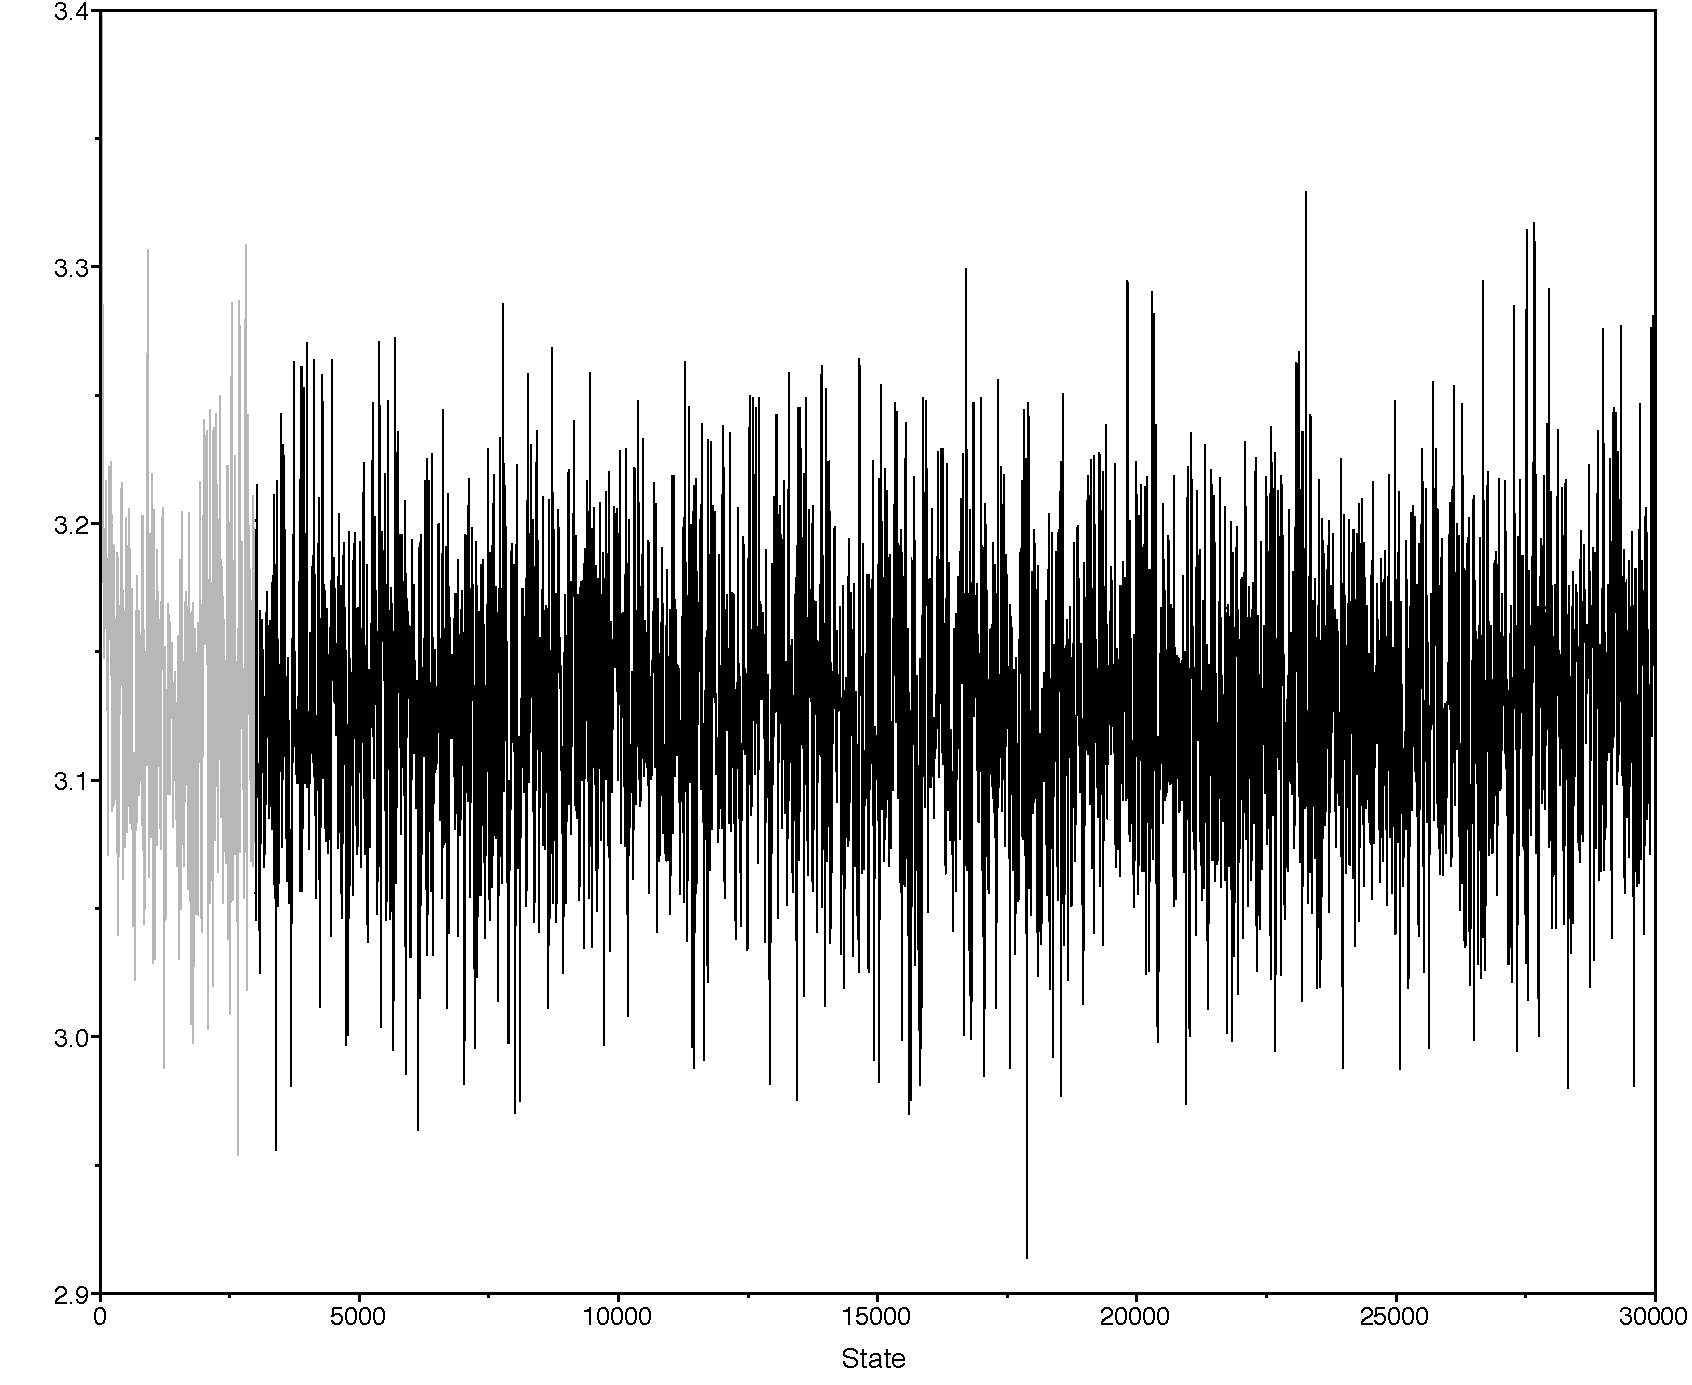
\includegraphics[width=0.4\textwidth]{\ResourcePath figures/primates_cytb_JC_TL_Trace.pdf}
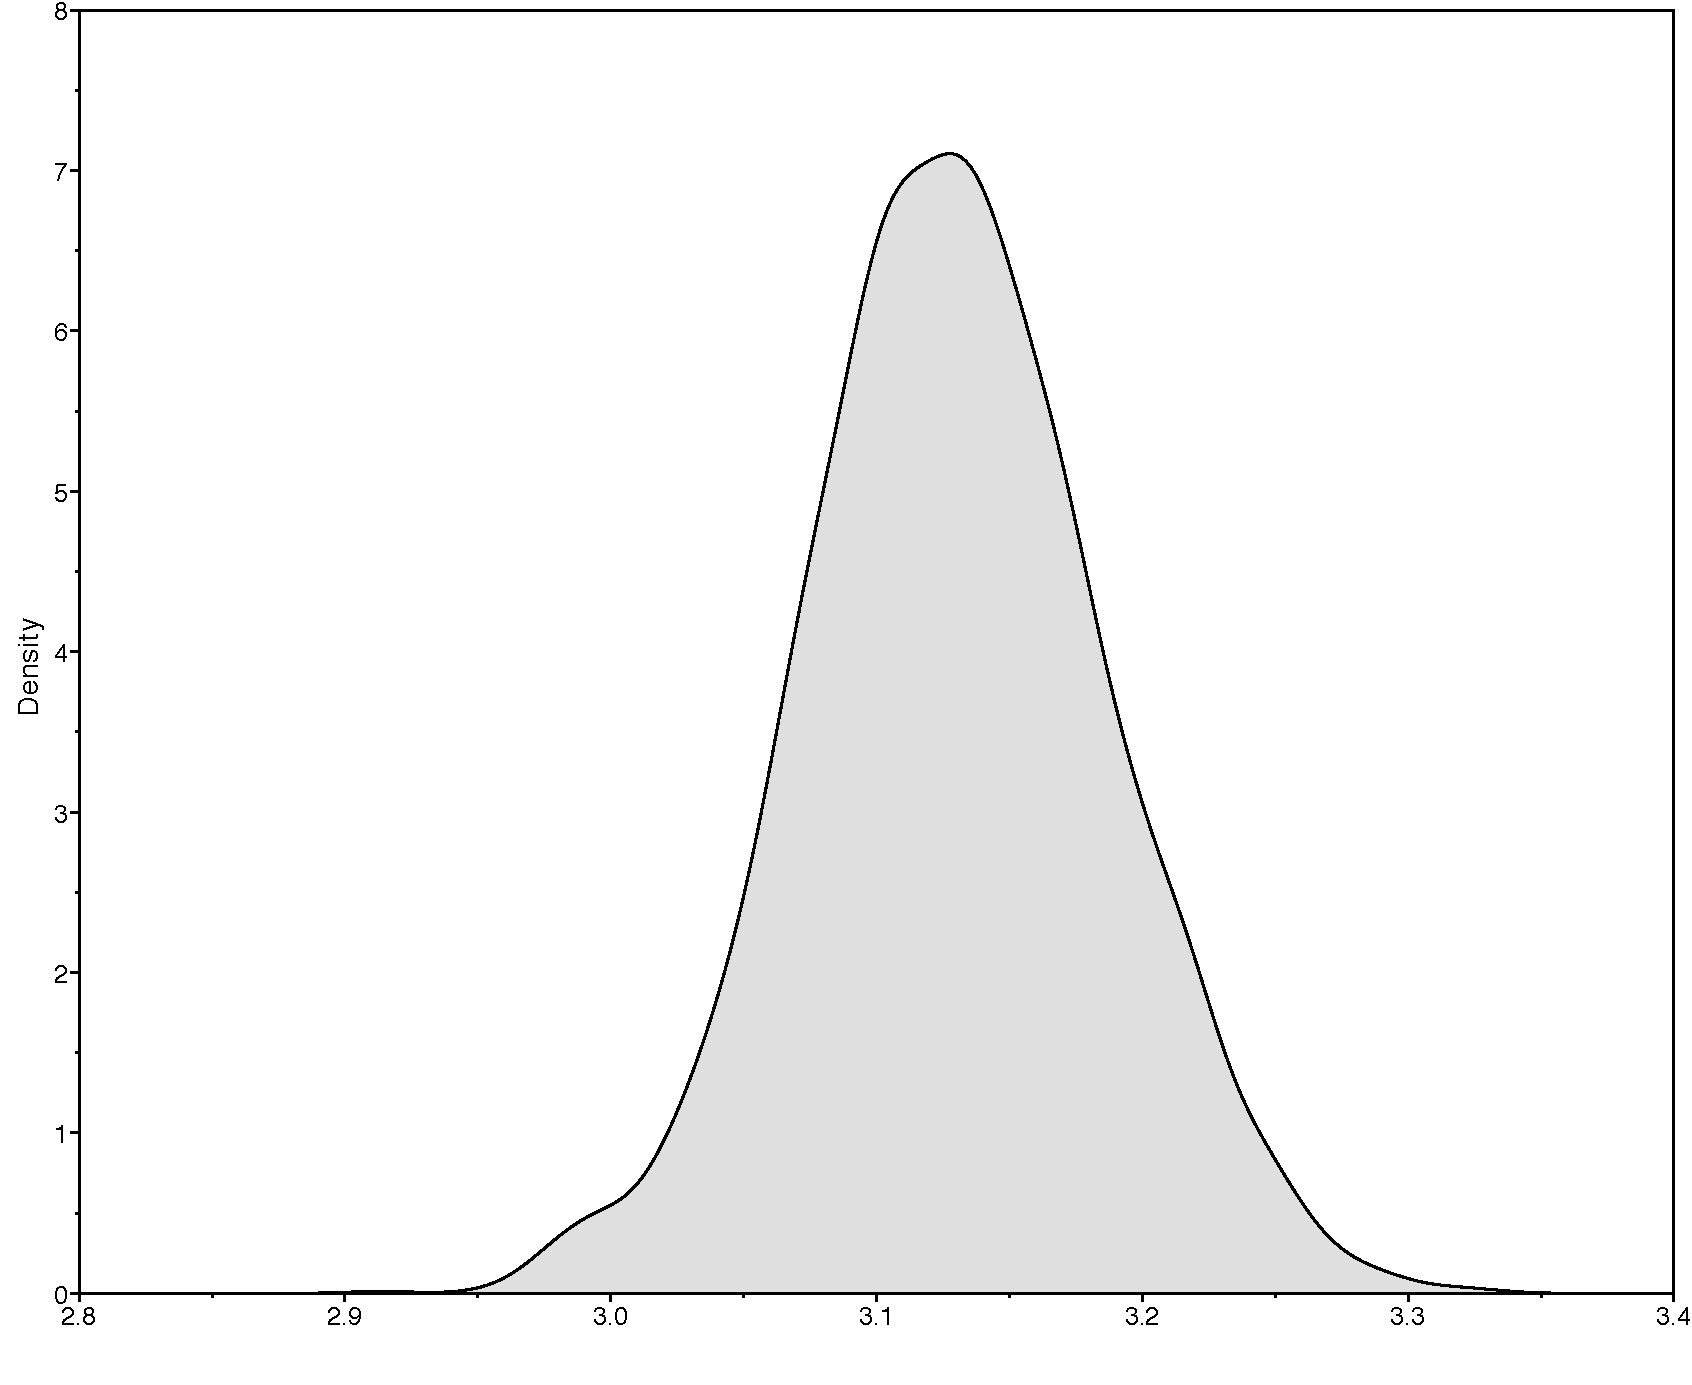
\includegraphics[width=0.4\textwidth]{\ResourcePath figures/primates_cytb_JC_TL_Distribution.pdf}}
\caption{\small Left: Trace of tree-length samples for one MCMC run. 
The caterpillar-like look is a good sign.
You will also see that the effective sample size is comparably large, \IE much larger than 200.
Right: Posterior distribution of the tree length of the primate phylogeny under a Jukes-Cantor substitution model.}
\label{fig:jc_tree}
\end{figure}

\subsection{Exercise 1}

We are interested in the phylogenetic relationship of the Tarsiers. Therefore, we need to summarize the trees sampled from the posterior distribution.
\RevBayes can summarize the sampled trees by reading in the tree-trace file:
{\tt \begin{snugshade*}
\begin{lstlisting}
treetrace = readTreeTrace("output/primates_cytb_JC.trees", treetype="non-clock")
\end{lstlisting}
\end{snugshade*}}
The \cl{mapTree()} function will summarize the tree samples and write the maximum \textit{a posteriori} tree to file:
{\tt \begin{snugshade*}
\begin{lstlisting}
map_tree = mapTree(treetrace,"output/primates_cytb_JC_MAP.tree")
\end{lstlisting}
\end{snugshade*}}
\begin{figure}[htbp!]
\centering
\fbox{\includegraphics[width=0.8\textwidth]{\ResourcePath figures/primates_cytb_JC_tree.pdf}}
\caption{\small Maximum a posteriori estimate of the primate phylogeny under a Jukes-Cantor substitution model. 
The numbers at the nodes show the posterior probabilities for the clades.
We have rooted the tree at the outgroup \emph{Galeopterus\_variegatus}}
\label{fig:jc_tree}
\end{figure}
\noindent \\ \impmark Look at the file called \cl{output/primates\_cytb\_JC\_MAP.tree} in \texttt{FigTree}. We show it in Figure~\ref{fig:jc_tree}.

\pagebreak
\noindent \impmark Fill in the following table as you go through the tutorial.

Note, you can query the posterior probability of a clade being monophyletic using the following command:
{\tt \begin{snugshade*}
\begin{lstlisting}
Lemuroidea <- clade("Cheirogaleus_major", 
                    "Daubentonia_madagascariensis", 
                    "Lemur_catta", 
                    "Lepilemur_hubbardorum",
                    "Microcebus_murinus",
                    "Propithecus_coquereli",
                    "Varecia_variegata_variegata")
                    
treetrace.cladeProbability( Lemuroidea )
\end{lstlisting}
\end{snugshade*}}

\begin{Form}
\begin{table}[h!]
\centering
\caption{\small Posterior probabilities of primate phylogenetic relationships$^*$.}
\resizebox{\textwidth}{!}{%
\begin{tabular}{l c c c c}
\hline
\textbf{Model} & \textbf{Lemuroidea} & \textbf{Lorisoidea} & \textbf{Platyrrhini} & \textbf{Catarrhini} \\ 
\hline
\vspace{1mm}
Jukes-Cantor & \TextField[name=pp11,backgroundcolor={.85 .85 .85},color={1 0 0},height=4ex]{}  & \TextField[name=pp12,backgroundcolor={.85 .85 .85},color={0 0 1},height=4ex]{}  & \TextField[name=pp13,backgroundcolor={.85 .85 .85},color={0 0 1},height=4ex]{}  & \TextField[name=pp14,backgroundcolor={.85 .85 .85},color={0 0 1},height=4ex]{}\\
\hline
\vspace{1mm}
HKY85 & \TextField[name=pp21,backgroundcolor={.85 .85 .85},color={1 0 0},height=4ex]{}  & \TextField[name=pp22,backgroundcolor={.85 .85 .85},color={0 0 1},height=4ex]{}  & \TextField[name=pp23,backgroundcolor={.85 .85 .85},color={0 0 1},height=4ex]{}  & \TextField[name=pp24,backgroundcolor={.85 .85 .85},color={0 0 1},height=4ex]{} \\
\hline
\vspace{1mm}
F81 & \TextField[name=pp31,backgroundcolor={.85 .85 .85},color={1 0 0},height=4ex]{}  & \TextField[name=pp32,backgroundcolor={.85 .85 .85},color={0 0 1},height=4ex]{}  & \TextField[name=pp33,backgroundcolor={.85 .85 .85},color={0 0 1},height=4ex]{}  & \TextField[name=pp34,backgroundcolor={.85 .85 .85},color={0 0 1},height=4ex]{} \\
\hline
\vspace{1mm}
GTR & \TextField[name=pp41,backgroundcolor={.85 .85 .85},color={1 0 0},height=4ex]{}  & \TextField[name=pp42,backgroundcolor={.85 .85 .85},color={0 0 1},height=4ex]{}  & \TextField[name=pp43,backgroundcolor={.85 .85 .85},color={0 0 1},height=4ex]{}  & \TextField[name=pp44,backgroundcolor={.85 .85 .85},color={0 0 1},height=4ex]{} \\
\hline
\vspace{1mm}
GTR+$\Gamma$ & \TextField[name=pp51,backgroundcolor={.85 .85 .85},color={1 0 0},height=4ex]{}  & \TextField[name=pp52,backgroundcolor={.85 .85 .85},color={0 0 1},height=4ex]{}  & \TextField[name=pp53,backgroundcolor={.85 .85 .85},color={0 0 1},height=4ex]{}  & \TextField[name=pp54,backgroundcolor={.85 .85 .85},color={0 0 1},height=4ex]{} \\
\hline
\vspace{1mm}
GTR+$\Gamma$+I & \TextField[name=pp61,backgroundcolor={.85 .85 .85},color={1 0 0},height=4ex]{}  & \TextField[name=pp62,backgroundcolor={.85 .85 .85},color={0 0 1},height=4ex]{}  & \TextField[name=pp63,backgroundcolor={.85 .85 .85},color={0 0 1},height=4ex]{}  & \TextField[name=pp64,backgroundcolor={.85 .85 .85},color={0 0 1},height=4ex]{} \\
\hline
{\footnotesize{$^*$you can edit this table}}\\
\end{tabular}}
\label{tab:pp}
\end{table}
\end{Form}

\begin{table}[h!]
\centering
\caption{\small Primate species and famaly relationships.}
\begin{tabular}{l l l l}
\hline
\textbf{Species} & \textbf{Family} & \textbf{Parvorder} & \textbf{Suborder} \\ 
\hline
%Alouatta palliata & Atelidae & Platyrrhini (NWM) & Haplorrhini \\
Aotus trivirgatus & Aotidae & Platyrrhini (NWM) & Haplorrhini \\
Callicebus donacophilus & Pitheciidae & Platyrrhini (NWM) & Haplorrhini \\
Cebus albifrons & Cebidae & Platyrrhini (NWM) & Haplorrhini \\
Cheirogaleus major & Cheirogaleidae & Lemuroidea & Strepsirrhini \\
Chlorocebus aethiops & Cercopithecoidea & Catarrhini & Haplorrhini \\
Colobus guereza & Cercopithecoidea & Catarrhini & Haplorrhini \\
Daubentonia madagascariensis & Daubentoniidae & Lemuroidea & Strepsirrhini \\
Galago senegalensis & Galagidae & Lorisidae & Strepsirrhini \\
Hylobates lar & Hylobatidea & Catarrhini & Haplorrhini \\
Lemur catta & Lemuridae & Lemuroidea & Strepsirrhini \\
Lepilemur hubbardorum & Lepilemuridae & Lemuroidea & Strepsirrhini \\
Loris tardigradus & Lorisidae & Lorisidae & Strepsirrhini \\
Macaca mulatta & Cercopithecoidea & Catarrhini & Haplorrhini \\
Microcebus murinus & Cheirogaleidae & Lemuroidea & Strepsirrhini \\
Nycticebus coucang & Lorisidae & Lorisidae & Strepsirrhini \\
Otolemur crassicaudatus & Galagidae & Lorisidae & Strepsirrhini \\
Pan paniscus & Hominoidea & Catarrhini & Haplorrhini \\
Perodicticus potto & Lorisidae & Lorisidae & Strepsirrhini \\
Propithecus coquereli & Indriidae & Lemuroidea & Strepsirrhini \\
Saimiri sciureus & Cebidae & Platyrrhini (NWM) & Haplorrhini \\
Tarsius syrichta & Tarsiidae &  & Haplorrhini \\
Varecia variegata variegata & Lemuridae & Lemuroidea & Strepsirrhini \\
\hline
\end{tabular}
\label{tab:primates}
\end{table}




\newpage
\section{The Hasegawa-Kishino-Yano (HKY) 1985 Substitution Model}

The Jukes-Cantor model assumes that all substitution rates are equal, which also implies that the stationary frequencies of the four nucleotide bases are equal.
These assumptions are not very biologically reasonable, so we might wish to consider a more realistic substitution model that relaxes some of these assumptions.
For example, we might allow stationary frequencies, $\pi$, to be unequal, and allow rates of transition and transversion substitutions to differ, $\kappa$.
This corresponds to the substitution model proposed by \citet[][HKY]{Hasegawa1985}, which is specified with the following instantaneous-rate matrix: 
\begin{equation*}
Q_{HKY} = \begin{pmatrix} 
{\cdot} 			& {\pi_C} 	& {\kappa\pi_G} 			& {\pi_T} \\ 
{\pi_A} 		& {\cdot} 			& {\pi_C} 			& {\kappa\pi_T} \\ 
{\kappa\pi_A} 			& {\pi_C} 			& {\cdot} 			& {\pi_T} \\ 
{\pi_A} 			& {\kappa\pi_C} 			& {\pi_G} 	& {\cdot}  
\end{pmatrix} \mbox{  .}
\end{equation*}
[The diagonal ${\cdot}$ entries are equal to the negative sum of the elements in the corresponding row.] 

\noindent \\ \impmark Use the file \cl{mcmc\_JC.Rev} as a starting point for the HKY analysis.

Note that we are adding two new variables to our model.
We can define a variable \cl{pi} for the stationary frequencies that are drawn from a flat Dirichlet distribution by
{\tt \begin{snugshade*}
\begin{lstlisting}
pi_prior <- v(1,1,1,1) 
pi ~ dnDirichlet(pi_prior)
\end{lstlisting}
\end{snugshade*}}
Since \cl{pi} is a stochastic variable, we need to specify a move to propose updates to it.
A good move on variables drawn from a Dirichlet distribution is the \cl{mvBetaSimplex}.
This move randomly takes an element from the simplex, proposes a new value for it drawn from a Beta distribution, and then rescales all values of the simplex to sum to 1 again.
{\tt \begin{snugshade*}
\begin{lstlisting}
moves[mvi++] = mvBetaSimplex(pi, weight=2)
moves[mvi++] = mvDirichletSimplex(pi, weight=1)
\end{lstlisting}
\end{snugshade*}}

The second new variable is $\kappa$, which specifies the ratio of transition-transversion rates.
The $\kappa$ parameter must be a positive-real number and a natural choice as the prior distribution is the lognormal distribution:
{\tt \begin{snugshade*}
\begin{lstlisting}
kappa ~ dnLognormal(0.0, 1.0)
\end{lstlisting}
\end{snugshade*}}
Again, we need to specify a move for this new stochastic variable.
A simple scaling move should do the job.
{\tt \begin{snugshade*}
\begin{lstlisting}
moves[mvi++] = mvScale(kappa)
\end{lstlisting}
\end{snugshade*}}

Finally, we need to create the HKY instantaneous-rate matrix using the \cl{fnHKY} function:
{\tt \begin{snugshade*}
\begin{lstlisting}
Q := fnHKY(kappa,pi)
\end{lstlisting}
\end{snugshade*}}
This should be all for the HKY model.

\noindent \\ \impmark Don't forget to change the output file names, otherwise your old analyses files will be overwritten.

\subsection{Exercise 2}

\begin{itemize}
\item With figure \ref{fig:jc} as your guide, draw the probabilistic graphical model of the HKY model.
\item Copy the file called  \cl{mcmc\_JC.Rev} and modify it by including the necessary parameters to specify the HKY substitution model.
\item Run an MCMC analysis to estimate the posterior distribution under the HKY substitution model.
\item Are the resulting estimates of the base frequencies equal? 
	If not, how much do they differ? 
	Are the estimated base frequencies similar to the empirical base frequencies? 
	The empirical base frequencies are the frequencies of the characters in the alignment, which can be computed with \RevBayes by \cl{data.getEmpiricalBaseFrequencies()}.
\item Is the inferred rate of transition substitutions higher than the rate of transversion substitutions? If so, by how much?
\item Like the HKY model, the Felsenstein 1981 (F81) substitution model has unequal stationary frequencies, but it assumes equal transition-transversion rates \citep{Felsenstein1981}.
	Can you set up the F81 model and run an analysis?
\item Complete the Table \ref{tab:pp} by reporting the posterior probabilities of phylogenetic relationships.
\end{itemize}






\section{The General Time-Reversible (GTR) Substitution Model}

The HKY substitution model can accommodate unequal base frequencies and different rates of transition and transversion substitutions.
Despite these extensions, the HKY model may still be too simplistic for many real datasets.
Here, we extend the HKY model to specify the General Time Reversible (GTR) substitution model \citep{Tavare1986}, which allows all six exchangeability rates to differ (Figure \ref{fig:gtr}).

The instantaneous-rate matrix for the GTR substitution model is:
\begin{equation*}
\resizebox{4in}{!}{%  
$Q_{GTR} = \begin{pmatrix}
{\cdot}	   & {r_{AC}\pi_C} & {r_{AG}\pi_G} & {r_{AT}\pi_T} \\
{r_{AC}\pi_A} & {\cdot}       & {r_{CG}\pi_G} & {r_{CT}\pi_T} \\
{r_{AC}\pi_A} & {r_{CG}\pi_C} & {\cdot}       & {r_{GT}\pi_T} \\
{r_{AC}\pi_A} & {r_{CT}\pi_C} & {r_{GT}\pi_G} & {\cdot}       \\
\end{pmatrix} \mbox{  ,} $}
\end{equation*}

where the six exchangeability parameters, $r_{ij}$, specify the relative rates of change between states $i$ and $j$.  


\begin{figure}[h!]
\centering
\fbox{\includegraphics[width=\textwidth,angle=0]{\ResourcePath figures/gtr_graphical_model.pdf}}
\caption{\small Graphical model representation of the General Time Reversible (GTR) phylogenetic model.}
\label{fig:gtr}
\end{figure}

The GTR model requires that we define and specify a prior on the six exchangeability rates, which we will describe using a flat Dirichlet distribution.
As we did previously for the Dirichlet prior on base frequencies, we first define a constant node specifying the vector of concentration-parameter values using the \cl{v()} function:
{\tt \begin{snugshade*}
\begin{lstlisting}
er_prior <- v(1,1,1,1,1,1) 
\end{lstlisting}
\end{snugshade*}}
This node defines the concentration-parameter values of the Dirichlet prior distribution on the exchangeability rates. 
Now, we can create a stochastic node for the exchangeability rates using the \cl{dnDirichlet()} function, which takes the vector of concentration-parameter values as an argument and the \cl{\rbdn} operator. 
Together, these create a stochastic node named \cl{er} ($\theta$ in Figure \ref{fig:gtr}): 
{\tt \begin{snugshade*}
\begin{lstlisting}
er ~ dnDirichlet(er_prior)
\end{lstlisting}
\end{snugshade*}}


The Dirichlet distribution assigns probability densities to a group of parameters: e.g., those that measure proportions and must sum to 1. 
Here, we have specified a six-parameter Dirichlet prior, where each value describes one of the six relative rates of the GTR model: 
(1) $A\leftrightarrows C$; (2) $A\leftrightarrows G$; (3) $A\leftrightarrows T$; (4) $C\leftrightarrows G$; (5) $C\leftrightarrows T$; (6) $G\leftrightarrows T$. 
The input parameters of a Dirichlet distribution are called shape (or concentration) parameters. 
The expectation and variance for each variable are related to the sum of the shape parameters.
The prior we specified above is a `flat' or symmetric Dirichlet distribution; all of the shape parameters are equal (1,1,1,1,1,1).
This describes a model that allows for equal rates of change between nucleotides, such that the expected rate for each is equal to $\frac{1}{6}$ (Figure \ref{dirichletFig}a).
We might also parameterize the Dirichlet distribution such that all of the shape parameters were equal to 100, which would also specify a prior with an expectation of equal exchangeability rates (Figure \ref{dirichletFig}b). 
However, by increasing the values of the shape parameters, \cl{er\_prior <- v(100,100,100,100,100,100)}, the Dirichlet distribution will more strongly favor equal exchangeability rates; ({\it i.e.}, a relatively {\em informative} prior).
Alternatively, we might consider an asymmetric Dirichlet parameterization that could reflect a strong prior belief that transition and transversion substitutions occur at different rates.
For example, we might specify the prior density \cl{er\_prior <- v(4,8,4,4,8,4)}.   
Under this model, the expected rate for transversions would be $\frac{4}{32}$ and that for transitions would be $\frac{8}{32}$, and there would be greater prior probability on sets of GTR rates that matched this configuration (Figure \ref{dirichletFig}c). 
Yet another aymmetric prior could specify that each of the six GTR rates had a different value conforming to a Dirichlet(2,4,6,8,10,12). 
This would lead to a different prior probability density for each rate parameter (Figure \ref{dirichletFig}d).
Without strong prior knowledge about the pattern of relative rates, however, we can better reflect our uncertainty by using a vague prior on the GTR rates. 
Notably, all patterns of relative rates have the same probability density under \cl{er\_prior <- v(1,1,1,1,1,1)}.
\begin{figure}[h!]
\centering
\fbox{\includegraphics[width=5in]{\ResourcePath figures/dirichlet_rates.pdf}}
\caption{\small Four different examples of Dirichlet priors on exchangeability rates.}
\label{dirichletFig}
\end{figure}


For each stochastic node in our model, we must also specify a proposal mechanism if we wish to estimate that parameter. 
The Dirichlet prior on our parameter \cl{er} creates a \href{http://en.wikipedia.org/wiki/Simplex}{\textit{simplex}} of values that sum to 1. 

{\tt\small \begin{snugshade*}
\begin{lstlisting}
moves[mvi++] = mvBetaSimplex(er, weight=3)
moves[mvi++] = mvDirichletSimplex(er, weight=1)
\end{lstlisting}
\end{snugshade*}}

We can use the same type of distribution as a prior on the 4 stationary frequencies ($\pi_A, \pi_C, \pi_G, \pi_T$) since these parameters also represent proportions. 
Specify a flat Dirichlet prior density on the base frequencies:
{\tt \begin{snugshade*}
\begin{lstlisting}
pi_prior <- v(1,1,1,1) 
pi ~ dnDirichlet(pi_prior)
\end{lstlisting}
\end{snugshade*}}

The node \cl{pi} represents the $\pi$ node in Figure \ref{fig:gtr}.
Now add the simplex scale move on the stationary frequencies to the moves vector:
{\tt \small \begin{snugshade*}
\begin{lstlisting}
moves[mvi++] = mvBetaSimplex(pi, weight=2)
moves[mvi++] = mvDirichletSimplex(pi, weight=1)
\end{lstlisting}
\end{snugshade*}}

We can finish setting up this part of the model by creating a deterministic node for the GTR instantaneous-rate matrix \cl{Q}. 
The \cl{fnGTR()} function takes a set of exchangeability rates and a set of base frequencies to compute the instantaneous-rate matrix used when calculating the likelihood of our model.
{\tt \begin{snugshade*}
\begin{lstlisting}
Q := fnGTR(er,pi)
\end{lstlisting}
\end{snugshade*}}




\subsection{Exercise 3}

\begin{itemize}
\item Use one of your previous analysis files---either the \cl{mcmc\_JC.Rev} or \cl{HKY.Rev}---to specify a GTR analysis in a new file called \cl{mcmc\_GTR.Rev}.
	Adapt the old analysis to be performed under the GTR substitution model. 
\item Run an MCMC analysis to estimate the posterior distribution.
\item Complete the table of the phylogenetic relationship of primates.
\end{itemize}






\section{The Discrete Gamma Model of Among Site Rate Variation}


Members of the GTR family of substitution models assume that rates are homogeneous across sites, an assumption that is often violated by real data.
We can accommodate variation in substitution rate among sites (ASRV) by adopting the discrete-gamma model \citep{Yang1994a}.
This model assumes that the substitution rate at each site is a random variable that is described by a discretized gamma distribution, which has two parameters: the shape parameter, $\alpha$, and the rate parameter, $\beta$. 
In order that we can interpret the branch lengths as the expected number of substitutions per site, this model assumes that the mean site rate is equal to 1.
The mean of the gamma is equal to $\alpha/\beta$, so a mean-one gamma is specified by setting the two parameters to be equal, $\alpha=\beta$.
This means that we can fully describe the gamma distribution with the single shape parameter, $\alpha$. 
The degree of among-site substitution rate variation is inversely proportional to the value of the $\alpha$-shape parameter.
As the value of the $\alpha$-shape increases, the gamma distribution increasingly resembles a normal distribution with decreasing variance, which therefore corresponds to decreasing levels of ASRV (Figure \ref{asrhGammaFig}).
By contrast, when the value of the $\alpha$-shape parameter is $< 1$, the gamma distribution assumes a concave distribution that concentrates most of the prior density on low rates, but retains some prior mass on sites with very high rates, which therefore corresponds to high levels of ASRV (Figure \ref{asrhGammaFig}).
Note that, when $\alpha = 1$, the gamma distribution collapses to an exponential distribution with a rate parameter equal to $\beta$.


\begin{figure}[h]
\centering
\fbox{\includegraphics[width=3.5in]{\ResourcePath figures/asrh_gamma.pdf}}
\caption{\small The probability density of mean-one gamma-distributed rates for different values of the $\alpha$-shape parameter.}
\label{asrhGammaFig}
\end{figure}

We typically lack prior knowledge regarding the degree of ASRV for a given alignment.
Accordingly, rather than specifying a precise value of $\alpha$, we can instead estimate the value of the $\alpha$-shape parameter from the data.
This requires that we specify a diffuse (relatively `uninformative') prior on the $\alpha$-shape parameter.
For this analysis, we will use a lognormal distribution with a mean parameter, \cl{alpha\_prior\_mean}, equal to \cl{5.0}, and standard deviation, \cl{alpha\_prior\_sd}, equal to 0.587405 (thus, 95\% of the prior density spans exactly one order of magnitude).

This approach for accommodating ASRV is another example of a hierarchical model (Figure \ref{fig:gtrg}).
That is, variation in substitution rates across sites is addressed by applying a site-specific rate multiplier to each of the $j$ sites, $r_j$.
These rate-multipliers are drawn from a discrete, mean-one gamma distribution; the shape of this prior distribution (and the corresponding degree of ASRV) is governed by the $\alpha$-shape parameter.
The $\alpha$-shape parameter, in turn, is treated as a lognormal distributed random variable.
Finally, the shape of the lognormal prior is governed by the mean and standard deviation parameters, which are set to fixed values.   

\begin{figure}[h!]
\centering
\fbox{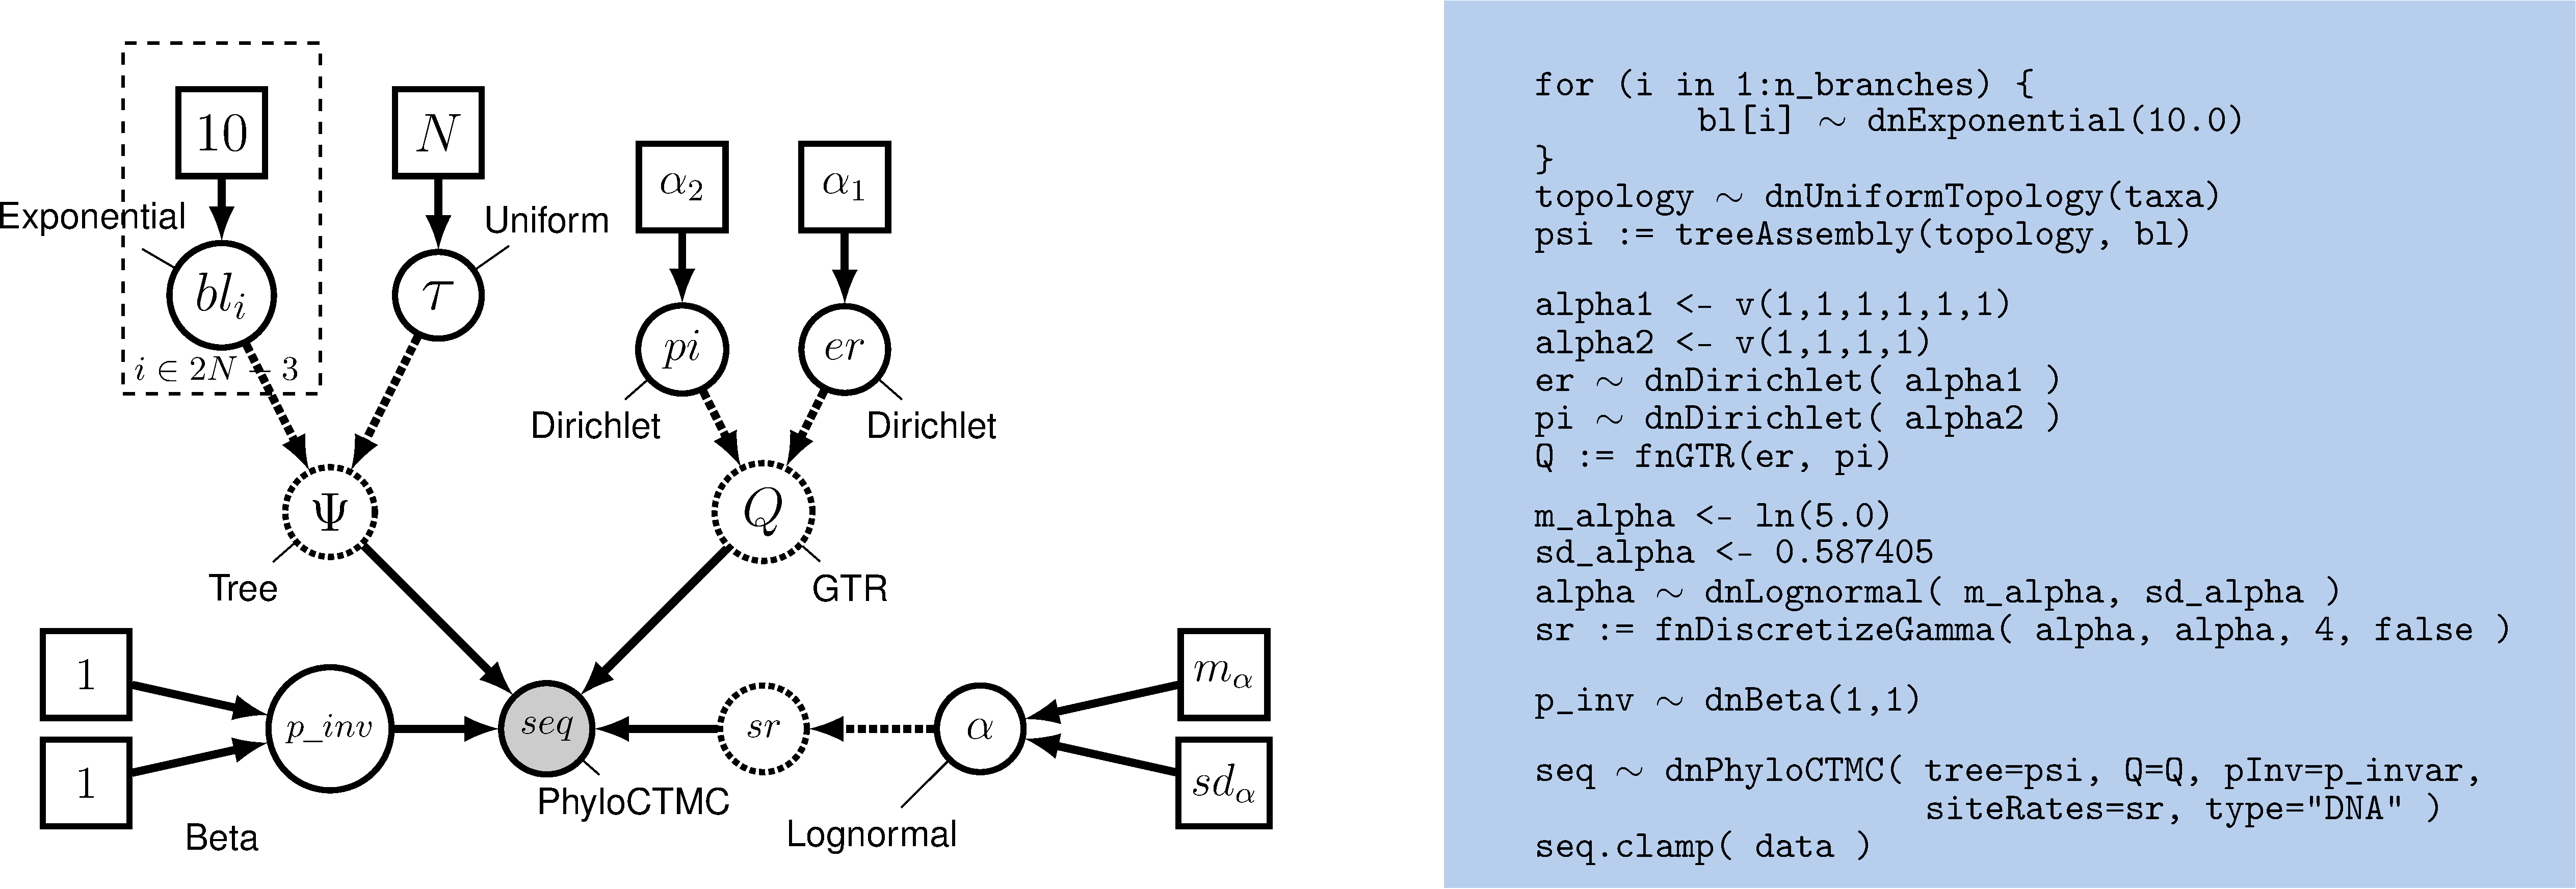
\includegraphics[width=\textwidth,angle=0]{\ResourcePath figures/gtrg_graphical_model.pdf}}
\caption{\small Graphical model representation of the General Time Reversible (GTR) + Gamma phylogenetic model with invariable sites.}
\label{fig:gtrg}
\end{figure}

\subsection{Setting up the Gamma Model in \RevBayes}

Create a constant node called \cl{alpha\_prior\_mean} for the mean parameter and a constant node called \cl{alpha\_prior\_sd} for the standard deviation of the lognormal prior on the gamma-shape parameter (this is represented as the constant $m_\alpha$ and $sd_\alpha$ parameters in Figure \ref{fig:gtrg}):
{\tt\begin{snugshade*}
\begin{lstlisting}
alpha_prior_mean <- ln(5.0)
alpha_prior_sd <- 0.587405
\end{lstlisting}
\end{snugshade*}}

Then create a stochastic node called \cl{alpha} with a lognormal prior (this represents the stochastic node for the $\alpha$-shape parameter in Figure \ref{fig:gtrg}):
{\tt\begin{snugshade*}
\begin{lstlisting}
alpha ~ dnLognormal( alpha_prior_mean, alpha_prior_sd )
\end{lstlisting}
\end{snugshade*}}

The way the ASRV model is implemented involves discretizing the mean-one gamma distribution into a set number of rate categories, $k$. 
Thus, we can analytically marginalize over the uncertainty in the rate at each site. 
The likelihood of each site is averaged over the $k$ rate categories, where the rate multiplier is the mean (or median) of each of the discrete $k$ categories. 
To specify this, we need a deterministic node that is a vector that will hold the set of $k$ rates drawn from the gamma distribution with $k$ rate categories. 
The \cl{fnDiscretizeGamma()} function returns this deterministic node and takes three arguments: the shape and rate of the gamma distribution and the number of categories. 
Since we want to discretize a mean-one gamma distribution, we can pass in \cl{alpha} for both the shape and rate.

Initialize the \cl{gamma\_rates} deterministic node vector using the  \cl{fnDiscretizeGamma()} function with \cl{4} bins:
{\tt \begin{snugshade*}
\begin{lstlisting}
gamma_rates := fnDiscretizeGamma( alpha, alpha, 4 )
\end{lstlisting}
\end{snugshade*}}

Note that here, by convention, we set $k = 4$.
The random variable that controls the rate variation is the stochastic node \cl{alpha}. 
We will apply a simple scale move to this parameter.
{\tt \begin{snugshade*}
\begin{lstlisting}
moves[mvi++] = mvScale(alpha, weight=2.0)
\end{lstlisting}
\end{snugshade*}}

Remember that you need to call the \cl{PhyloCTMC} constructor to include the new site-rate parameter:
{\tt \begin{snugshade*}
\begin{lstlisting}
seq ~ dnPhyloCTMC(tree=psi, Q=Q, siteRates=gamma_rates, type="DNA")
\end{lstlisting}
\end{snugshade*}}


\subsection{Exercise 4}

Modify the previous GTR analysis to specify the GTR+Gamma model. 
Run an MCMC simulation to estimate the posterior distribution.
\begin{itemize}
\item Is there an impact on the estimated phylogeny compared with the previous analyses? 
	Look at the MAP tree and the posterior probabilities of the clades.
\item Complete the table of the phylogenetic relationship of primates.
\end{itemize}



\newpage
\section{Modeling Invariable Sites}
All of the substitution models described so far assume that the sequence data are potentially variable.
That is, we assume that the sequence data are random variables; specifically, we assume that they are realizations of the specified \cl{PhyloCTMC} distribution. 
However, some sites may not be free to vary---when the substitution rate of a site is zero, it is said to be \emph{invariable}.
Invariable sites are often confused with \emph{invariant} sites---when each species exhibits the same state, it is said to be invariant.
The concepts are related but distinct.
If a site is truly invariable, it will necessarily give rise to an invariant site pattern, as such sites will always have a zero substitution rate.
However, an invariant site pattern may be achieved via multiple substitutions that happen to end in the same state for every species.

Here we describe an extension to our phylogenetic model to accommodate invariable sites.
Under the invariable-sites model \citep[][]{Hasegawa1985}, each site is invariable with probability \cl{pinvar}, and variable with probability $1-$\cl{pinvar}.

First, let's have a look at the data and see how many invariant sites we have:
{\tt \begin{snugshade*}
\begin{lstlisting}
data.getNumInvariantSites()
\end{lstlisting}
\end{snugshade*}}
There seem to be a substantial number of invariant sites.

Now let's specify the invariable-sites model in \RevBayes.
We need to specify the prior probability that a site is invariable.
A Beta distribution is a common choice for parameters representing probabilities.
{\tt \begin{snugshade*}
\begin{lstlisting}
pinvar ~ dnBeta(1,1)
\end{lstlisting}
\end{snugshade*}}
The \cl{Beta(1,1)} distribution is a flat prior distribution that specifies equal probability for all values between 0 and 1.

Then, as usual, we add a move to change this stochastic variable; we'll used a simple sliding window move.
{\tt \begin{snugshade*}
\begin{lstlisting}
moves[mvi++] = mvSlide(pinvar)
\end{lstlisting}
\end{snugshade*}}

Finally, you need to call the \cl{PhyloCTMC} constructor to include the new\cl{pinvar} parameter:
{\tt \begin{snugshade*}
\begin{lstlisting}
seq ~ dnPhyloCTMC(tree=psi, Q=Q, siteRates=gamma_rates, pInv=pinvar, type="DNA")
\end{lstlisting}
\end{snugshade*}}

\subsection{Exercise 5}

\begin{itemize}
\item Extend the GTR model to account for invariable sites and run an analysis.
\item What is the estimated probability of invariable sites and how does it relate to the ratio of invariant sites to the total number of sites?
\item Extend the GTR+$\Gamma$ model to account for invariable sites and run an analysis.
\item What is the estimated probability of invariable sites now?
\item Complete the table of the phylogenetic relationship of primates.
\end{itemize} 


\bibliographystyle{sysbio}
\bibliography{\GlobalResourcePath refs}


\chapter{Partitioned Data Analysis}
\def \ResourcePath {RB_Partition_Tutorial/}
\include{RB_Partition_Tutorial/RB_Partition_Tutorial_content}





\part{Divergence Time Estimation}

%\chapter{A Brief Introduction, Overview and Example of Dating, Calibration and Relaxed Clocks}
%\def \ResourcePath {RB_Dating_Tutorial/}
%\include{RB_Dating_Tutorial/RB_Dating_Tutorial_content}

\chapter{Overview}
\def \ResourcePath {RB_DivergenceTime_Tutorial/}
\include{RB_DivergenceTime_Tutorial/RB_DivergenceTime_Tutorial_content}

\chapter{Node and Fossil Calibration}
\def \ResourcePath {RB_DivergenceTime_Calibration_Tutorial/}
\include{RB_DivergenceTime_Calibration_Tutorial/RB_DivergenceTime_Calibration_Tutorial_content}

\chapter{Relaxed Clocks}
\def \ResourcePath {RB_DivergenceTime_RelaxedClock_Tutorial/}
\include{RB_DivergenceTime_RelaxedClock_Tutorial/RB_DivergenceTime_RelaxedClock_Tutorial_content}

%\chapter{Node Calibration}
%\def \ResourcePath {RB_NodeCalibration_Tutorial/}
%\include{RB_NodeCalibration_Tutorial/RB_NodeCalibration_Tutorial_content}




\part{Gene tree - Species tree estimation}

\chapter{Overview}
\def \ResourcePath {RB_GTST_Tutorial/}
\include{RB_GTST_Tutorial/RB_GTST_Tutorial_content}

\chapter{Estimating species tree using gene concatenation}
\def \ResourcePath {RB_GeneConcatenation_Tutorial/}
\include{RB_GeneConcatenation_Tutorial/RB_GeneConcatenation_Tutorial_content}

\chapter{Multispecies Coalescent}
\def \ResourcePath {RB_MultispeciesCoalescent_Tutorial/}
\include{RB_MultispeciesCoalescent_Tutorial/RB_MultispeciesCoalescent_Tutorial_content}



\part{Diversification Rate Estimation}

\chapter{Overview}
\def \ResourcePath {RB_DiversificationRateIntro_Tutorial/}
\include{RB_DiversificationRateIntro_Tutorial/RB_DiversificationRateIntro_Tutorial_content}

\chapter{Basic Diversification Rate Estimation}
\def \ResourcePath {RB_DiversificationRate_Tutorial/}
\include{RB_DiversificationRate_Tutorial/RB_DiversificationRate_Tutorial_content}

\chapter{Episodic Diversification Rate Estimation}
\def \ResourcePath {RB_DiversificationRate_Episodic_Tutorial/}
\section{Estimating Speciation \& Extinction Rates Through Time}

\subsection{Outline}

This tutorial describes how to specify an episodic branching-process model in \RevBayes; a birth-death process where diversification rates vary episodically through time modeled as piecewise-constant rates \citep{Stadler2011,Hoehna2015a}.
The probabilistic graphical model is given once at the beginning of this tutorial.
Your goal is to estimate speciation and extinction rates through-time using Markov chain Monte Carlo (MCMC).


\subsection{Requirements}
We assume that you have read and hopefully completed the following tutorials:
\begin{itemize}
\item \href{https://github.com/revbayes/revbayes_tutorial/raw/master/tutorial_TeX/RB_Getting_Started/RB_Getting_Started.pdf}{Getting started}
\item \href{https://github.com/revbayes/revbayes_tutorial/raw/master/tutorial_TeX/RB_Intro_Tutorial/RB_Intro_Tutorial.pdf}{Very Basic Introduction to \Rev}
\item \href{https://github.com/revbayes/revbayes_tutorial/raw/master/tutorial_TeX/RB_Rev_Tutorial/RB_Rev_Tutorial.pdf}{General Introduction to the \Rev syntax}
\item \href{https://github.com/revbayes/revbayes_tutorial/raw/master/tutorial_TeX/RB_MCMC_Archery_Tutorial/RB_MCMC_Archery_Tutorial.pdf}{General Introduction to MCMC using an archery example}
\item \href{https://github.com/revbayes/revbayes_tutorial/raw/master/tutorial_TeX/RB_MCMC_Binomial_Tutorial/RB_MCMC_Binomial_Tutorial.pdf}{General Introduction to MCMC using a coin-flipping example}
\item \href{https://github.com/revbayes/revbayes_tutorial/raw/master/tutorial_TeX/RB_DiversificationRate_Tutorial/RB_DiversificationRate_Tutorial.pdf}{Basic Diversification Rate Estimation}
\end{itemize}
Note that the \href{https://github.com/revbayes/revbayes_tutorial/raw/master/tutorial_TeX/RB_Intro_Tutorial/RB_Intro_Tutorial.pdf}{\Rev basics tutorial} introduces the basic syntax of \Rev but does not cover any phylogenetic models.
We tried to keep this tutorial very basic and introduce all the language concepts and theory on the way.
You may only need the \href{https://github.com/revbayes/revbayes_tutorial/raw/master/tutorial_TeX/RB_Rev_Tutorial/RB_Rev_Tutorial.pdf}{\Rev syntax tutorial} for a more in-depth discussion of concepts in \Rev.


%%%%%%%%
%%   Data   %%
%%%%%%%%
\section{Data and files}

We provide the data file(s) which we will use in this tutorial.
You may want to use your own data instead.
In the \cl{data} folder, you will find the following files
\begin{itemize}
\item \cl{primates\_tree.nex}: Dated primates phylogeny including 233 out of 367 species from \cite{MagnusonFord2012}.
\end{itemize}


\impmark{Open the tree \cl{data/primates\_tree.nex} in \FigTree.}


\bigskip
\section{Episodic Birth-Death Model}

The basic idea behind the model is that speciation and extinction rates are constant within time intervals but can be different between time intervals.
Thus, we will divide time into equally sized intervals, with the only exception that the first 20\% of the time does not have any rate changes.
Our only reason to do so is because there are too few lineages in the reconstructed tree at that time to obtain reliable parameter estimates.
An overview of the underlying theory of the specific model and implementation is given in \cite{Hoehna2015a}.
\begin{figure}[h!]
\centering
\fbox{\includegraphics[width=\textwidth]{\ResourcePath figures/EBD_scenarios.pdf}}
\caption{\small Two scenarios of birth-death models. On the left we show constant diversification. On the right we show an example of an episodic birth-death process where rates are constant in each time interval (epoch). The top panel of this figure shows an example realization under the given rates.}
\label{fig:EBD}
\end{figure}
Figure~\ref{fig:EBD} shows an example of a constant rate birth-death process and an episodic birth-death process.

We assume that the log-transformed rates are drawn from a normal distribution.
Furthermore, we will assume that rates are autocorrelated, that is, rates in the current time interval will be centered around the rates in the previous time interval.
Thus, we model (log-transformed) diversification rates by a Brownian motion.
The assumption of autocorrelated rates does not only makes sense biologically but also improves our ability to estimate parameters.
\begin{figure}[h!]
\centering
\fbox{\includegraphics[width=\textwidth]{\ResourcePath figures/graphical_model_EBD.pdf}}
\caption{\small A graphical model with the outline of the \Rev code. On the left we see the graphical model describing the correlated (Brownian motion) model for rate-variation through time. On the right we show the corresponding \Rev commands to instantiate this model. This figure gives a complete overview of the model that we use here in this analysis.}
\label{fig:EBD_GM}
\end{figure}
We show a graphical model of the episodic birth-death process with autocorrelated rates in Figure~\ref{fig:EBD_GM}.
This graphical model shows you which variables are included in the model, and the dependency between the variables.
Thus, it makes the structure and assumption of the model clear and visible instead of a black-box \citep{Hoehna2014b}.
For example, you see how the speciation and extinction rates in each time interval depend on the rates of the previous interval, and that we use a hyperprior for the standard deviation of rates between time intervals.


\subsection{Read the tree}

Begin by reading in the ``observed'' tree.

{\tt \begin{snugshade*}
\begin{lstlisting}
T <- readTrees("data/primates_tree.nex")[1]
\end{lstlisting}
\end{snugshade*}}

From this tree, we get some helpful variables, such as the taxon information which we need to instantiate the birth-death process.
{\tt \begin{snugshade*}
\begin{lstlisting}
taxa <- T.taxa()
\end{lstlisting}
\end{snugshade*}}

Additionally, we initialize an iterator variable for our vector of moves and monitors.
{\tt \begin{snugshade*}
\begin{lstlisting}
mvi = 0
mni = 0
\end{lstlisting}
\end{snugshade*}}

Finally, we create a helper variable that specifies the number of intervals.
{\tt \begin{snugshade*}
\begin{lstlisting}
NUM_INTERVALS = 10
\end{lstlisting}
\end{snugshade*}}
Using this variable we can easily change our script to break-up time into many (\EG~\cl{NUM\_INTERVALS = 100}) or few (\EG~\cl{NUM\_INTERVALS = 4}) intervals.



\subsection{Specifying the model}

\subsubsection{Priors on amount of rate variation}
We start by specifying prior distributions on the rates.
Each interval-specific speciation- and extinction-rate will be drawn from a normal distribution.
Thus, we need a parameter for the standard deviation of those normal distributions.
We use an exponential hyperprior with rate 1.0 to estimate the standard deviation, but assume that all speciation rates and all extinction rates share the same standard deviation.
The motivation for an exponential hyperprior is that it has the highest probability density at 0 which would make the variance of rates between consecutive time intervals 0 and thus represent a constant-rate process.
The data will tell us if there should be much variation in rates through time.
(You may want to experiment with this hyperprior if you are interested.)
{\tt \begin{snugshade*}
\begin{lstlisting}
speciation_sd ~ dnExponential(1.0)
extinction_sd ~ dnExponential(1.0)
\end{lstlisting}
\end{snugshade*}}
We apply a simple scaling move on each prior parameter.
{\tt \begin{snugshade*}
\begin{lstlisting}
moves[++mvi] = mvScale(speciation_sd,weight=5.0)
moves[++mvi] = mvScale(extinction_sd,weight=5.0)
\end{lstlisting}
\end{snugshade*}}



\subsubsection{Specifying episodic rates}
As we mentioned before, we will apply normal distributions as priors for each log-transformed rate.
We begin with the rate at the present which is our initial rate parameter.
The rates at the present will be specified slightly differently because they are not correlated to any previous rates.
This is because we are actually modeling rate-changes backwards in time and there is no previous rate for the rate at the present.
Modeling rates backwards in time makes it easier for us if we had some prior information about some event affected diversification sometime before the present, \EG 25 million years ago.

We use a uniform distribution between -10 and 10 because of our lack of prior knowledge on the diversification rate.
This actually means that we allow speciation and extinction rates between $e^{-10}$ and $e^10$, so we should clearly cover the true values.
(Note that for diversification rate estimates, $e^{-10}$ is virtually 0 since the rate is so slow).
{\tt \begin{snugshade*}
\begin{lstlisting}
log_speciation[1] ~ dnUniform(-10.0,10.0)
log_speciation[1] ~ dnUniform(-10.0,10.0)
\end{lstlisting}
\end{snugshade*}}
Notice that we store the diversification rate variables in vectors.
Storing the rate parameters in vectors will be useful and important later when we pass the rates into the birth-death process.

We apply simple sliding window moves for the rates.
Normally we would use scaling moves but in this case we work on the log-transformed parameters and thus sliding moves perform better.
(If you are keen you can test the differences.)
{\tt \begin{snugshade*}
\begin{lstlisting}
moves[++mvi] = mvSlide(log_speciation[1], weight=2)
moves[++mvi] = mvSlide(log_extinction[1], weight=2)
\end{lstlisting}
\end{snugshade*}}
Now we transform the diversification rate parameters into actual rates using an exponential parameter transformation.
{\tt \begin{snugshade*}
\begin{lstlisting}
speciation[1] := exp( log_speciation[1] )
extinction[1] := exp( log_extinction[1] )
\end{lstlisting}
\end{snugshade*}}

Next, we specify the speciation and extinction rates for each time interval (\IE epoch).
This can be done efficiently using a \cl{for}-loop.
We will use a specific index variable so that we can more easily refer to the rate at the previous interval.
Remember that we want to model the rates as a Brownian motion, which we achieve by specifying a normal distribution as the prior distribution on the rates centered around the previous rate (\IE the mean of the normal distribution is equal to the previous rate).
{\tt \begin{snugshade*}
\begin{lstlisting}
for (i in 1:NUM_INTERVALS) {
    index = i+1

    log_speciation[index] ~ dnNormal( mean=log_speciation[i], sd=speciation_sd )
    log_extinction[index] ~ dnNormal( mean=log_extinction[i], sd=extinction_sd )

    moves[++mvi] = mvSlide(log_speciation[index], weight=2)
    moves[++mvi] = mvSlide(log_extinction[index], weight=2)

    speciation[index] := exp( log_speciation[index] )
    extinction[index] := exp( log_extinction[index] )

}
\end{lstlisting}
\end{snugshade*}}
Finally, we apply moves that slide all values in the rate vectors, \IE all speciation or extinction rates.
We will use an \cl{mvVectorSlide} move.
{\tt \begin{snugshade*}
\begin{lstlisting}
moves[++mvi] = mvVectorSlide(log_speciation, weight=10)
moves[++mvi] = mvVectorSlide(log_extinction, weight=10)
\end{lstlisting}
\end{snugshade*}}

Additionally, we apply a \cl{mvShrinkExpand} move which changes the spread of several variables around their mean.
{\tt \begin{snugshade*}
\begin{lstlisting}
moves[++mvi] = mvShrinkExpand( log_speciation, sd=speciation_sd, weight=10 )
moves[++mvi] = mvShrinkExpand( log_extinction, sd=extinction_sd, weight=10 )
\end{lstlisting}
\end{snugshade*}}
Both moves considerably improve the efficiency of our MCMC analysis.

\subsubsection{Setting up the time intervals}
In \RevBayes you actually have the possibility to specify unequal time intervals or even different intervals for the speciation and extinction rate.
This is achieved by providing a vector of times when each interval ends.
Here we simply break-up the most recent 80\% of time since the root in equal-length intervals.
{\tt \begin{snugshade*}
\begin{lstlisting}
interval_times <- T.rootAge() * (1:NUM_INTERVALS) / (NUM_INTERVALS) * 0.8
\end{lstlisting}
\end{snugshade*}}
This vector of times will be used for both the speciation and extinction rates.
Also, remember that the times of the intervals represent ages going backwards in time.

\subsubsection{Incomplete Taxon Sampling}

We know that we have sampled 233 out of 367 living primate species.
To account for this we can set the sampling parameter as a constant node with a value of 233/367.
For simplicity, and since almost all species have been sampled, we assume \emph{uniform} taxon sampling \citep{Hoehna2011,Hoehna2014a},
{\tt \begin{snugshade*}
\begin{lstlisting}
rho <- T.ntips()/367
\end{lstlisting}
\end{snugshade*}}


\subsubsection{Root age}

The birth-death process requires a parameter for the root age.
In this exercise we use a fixed tree and thus we know the age of the tree.
Hence, we can get the value for the root from the \citet{MagnusonFord2012} tree.
{\tt \begin{snugshade*}
\begin{lstlisting}
root_time <- T.rootAge()
\end{lstlisting}
\end{snugshade*}}

\subsubsection{The time tree}

Now we have all of the parameters we need to specify the full episodic birth-death model.
We initialize the stochastic node representing the time tree.
{\tt \begin{snugshade*}
\begin{lstlisting}
timetree ~ dnEpisodicBirthDeath(rootAge=T.rootAge(), lambdaRates=speciation, lambdaTimes=interval_times, muRates=extinction, muTimes=interval_times, rho=rho, samplingStrategy="uniform", condition="survival", taxa=taxa)
\end{lstlisting}
\end{snugshade*}}
You may notice that we explicitly specify that we want to condition on survival.
It is possible to change this condition to the \emph{time of the process} or \emph{the number of sampled taxa} too.

Then we attach data to the \cl{timetree} variable.
{\tt \begin{snugshade*}
\begin{lstlisting}
timetree.clamp(T)
\end{lstlisting}
\end{snugshade*}}

Finally, we create a workspace object of our whole model using the \cl{model()} function.
{\tt \begin{snugshade*}
\begin{lstlisting}
mymodel = model(speciation)
\end{lstlisting}
\end{snugshade*}}

The \cl{model()} function traversed all of the connections and found all of the nodes we specified.


\subsection{Running an MCMC analysis}

\subsubsection{Specifying Monitors}

For our MCMC analysis, we need to set up a vector of \textit{monitors} to record the states of our Markov chain.
First, we will initialize the model monitor using the \cl{mnModel} function. This creates a new monitor variable that will output the states for all model parameters when passed into a MCMC function.
{\tt \begin{snugshade*}
\begin{lstlisting}
monitors[++mni] = mnModel(filename="output/primates_EBD.log",printgen=10, separator = TAB)
\end{lstlisting}
\end{snugshade*}}

Additionally, we create four separate file monitors, one for each vector of speciation and extinction rates and for each speciation and extinction rate epoch (\IE the times when the interval ends).
We want to have the speciation and extinction rates stored separately so that we can plot them nicely afterwards.
{\tt \begin{snugshade*}
\begin{lstlisting}
monitors[++mni] = mnFile(filename="output/primates_EBD_speciation_rates.log",printgen=10, separator = TAB, speciation)
monitors[++mni] = mnFile(filename="output/primates_EBD_speciation_times.log",printgen=10, separator = TAB, interval_times)
monitors[++mni] = mnFile(filename="output/primates_EBD_extinction_rates.log",printgen=10, separator = TAB, extinction)
monitors[++mni] = mnFile(filename="output/primates_EBD_extinction_times.log",printgen=10, separator = TAB, interval_times)
\end{lstlisting}
\end{snugshade*}}

Finally, we create a screen monitor that will report the states of specified variables to the screen with \cl{mnScreen}:
{\tt \begin{snugshade*}
\begin{lstlisting}
monitors[++mni] = mnScreen(printgen=1000, extinction_sd, speciation_sd)
\end{lstlisting}
\end{snugshade*}}

\subsubsection{Initializing and Running the MCMC Simulation}

With a fully specified model, a set of monitors, and a set of moves, we can now set up the MCMC algorithm that will sample parameter values in proportion to their posterior probability.
The \cl{mcmc()} function will create our MCMC object:
{\tt \begin{snugshade*}
\begin{lstlisting}
mymcmc = mcmc(mymodel, monitors, moves)
\end{lstlisting}
\end{snugshade*}}

First, we will run a pre-burnin to tune the moves and to obtain starting values from the posterior distribution.
{\tt \begin{snugshade*}
\begin{lstlisting}
mymcmc.burnin(generations=10000,tuningInterval=200)
\end{lstlisting}
\end{snugshade*}}


Now, run the MCMC:
{\tt \begin{snugshade*}
\begin{lstlisting}
mymcmc.run(generations=50000)
\end{lstlisting}
\end{snugshade*}}

When the analysis is complete, you will have the monitored files in your output directory.
You can then visualize the rates through time using \R using our package \RevGadgets.
If you don't have the R-package \RevGadgets installed, or if you have trouble with the package, then please read the separate tutorial about the package.

Just start \R in the main directory for this analysis and then type the following commands:
{\tt \begin{snugshade*}
\begin{lstlisting}
library(RevGadgets)

tree <- read.nexus("data/primates_tree.nex")

rev_out <- rev.process.div.rates(speciation_times_file = "output/primates_EBD_speciation_times.log", speciation_rates_file = "output/primates_EBD_speciation_rates.log", extinction_times_file = "output/primates_EBD_extinction_times.log", extinction_rates_file = "output/primates_EBD_extinction_rates.log", tree, burnin=0.25,numIntervals=100)

pdf("EBD.pdf")
par(mfrow=c(2,2))
rev.plot.output(rev_out,use.geoscale=FALSE)
dev.off()
\end{lstlisting}
\end{snugshade*}}
(Note, you may want to add a nice geological timescale to the plot by setting \cl{use.geoscale=TRUE} but then you can only plot one figure per page.)

\impmark{The \Rev file for performing this analysis: \href{https://github.com/revbayes/revbayes_tutorial/raw/master/RB_DiversificationRate_Episodic_Tutorial/scripts/mcmc_EBD.Rev}{\cl{mcmc\_EBD.Rev}}.}

\begin{figure}[h!]
\centering
\fbox{\includegraphics[width=\textwidth]{\ResourcePath figures/EBD_10_Result.pdf}}
\caption{\small Resulting diversification rate estimations when using 10 intervals. You should obtain similar results when you use 10 intervals. The estimated rates might change when you use a different resolution, \IE a different number of intervals.}
\label{fig:EBD_Results}
\end{figure}

\subsection{Exercise 1}

\begin{itemize}
\item Run an MCMC simulation to estimate the posterior distribution of the speciation rate and extinction rate.
\item Visualize the rate through time using \R.
\item Do you see evidence for rate decreases or increases? What is the general trend?
\item Is there evidence for rate variation? Look at the estimates of \cl{speciation\_sd} and \cl{extinction\_sd}: Is there information in the data to change the estimates from the prior?
\item Run the analysis using a different number of intervals, \EG 5 or 50. How do the rates change?
\end{itemize}


\subsection{Exercise 2}

\begin{itemize}
\item In our results we see that the extinction rate is fairly constant. Modify the model by using a constant-rate for the extinction rate parameter but still let the speciation rate vary through time.
\begin{itemize}
\item Remove all previous occurrences of the extinction rates (\IE priors, parameters and moves).
\item Specify a lognormal prior distribution on the constant extinction rate \\(\cl{extinction $\sim$ dnLognormal(-5,sd=2*0.587405)})
\item Add a move for the new extinction rate parameter \\\cl{moves[++mvi] = mvScale(extinction,weight=5.0)}.
\item Remove the argument \cl{muTimes=interval\_times} from the birth-death process.
\end{itemize}
\item How does this influence your estimated rates?
\end{itemize}



\bibliographystyle{sysbio}
\bibliography{\GlobalResourcePath refs}


\chapter{Environmental-correlated Diversification Rate Estimation}
\def \ResourcePath {RB_DiversificationRate_Environmental_Tutorial/}
\section{Estimating Environmental-dependent Speciation \& Extinction Rates}

\subsection{Outline}

This tutorial describes how to specify a branching-process model with diversification rate correlated with an environmental variable in \RevBayes.
Diversification rates are assumed to be equal among all lineages but vary through time correlated with an environmental predictor variable.
Thus, this model can be used to test for correlations between diversification rates and environmental variables, such as \COO and temperature.
However, these tests are only to establish a correlation, not a causality.

As usual, we provide the probabilistic graphical model at the beginning of this tutorial.
Hopefully this will help you to get a better idea of all the variables in the model and their dependencies.
Our goal in this tutorial is to estimate the correlation coefficient between speciation and extinction rates to historical \COO measurements using Markov chain Monte Carlo (MCMC).


\subsection{Requirements}
We assume that you have read and hopefully completed the following tutorials:
\begin{itemize}
\item \href{https://github.com/revbayes/revbayes_tutorial/raw/master/tutorial_TeX/RB_Getting_Started/RB_Getting_Started.pdf}{Getting started}
\item \href{https://github.com/revbayes/revbayes_tutorial/raw/master/tutorial_TeX/RB_Intro_Tutorial/RB_Intro_Tutorial.pdf}{Very Basic Introduction to \Rev}
\item \href{https://github.com/revbayes/revbayes_tutorial/raw/master/tutorial_TeX/RB_Rev_Tutorial/RB_Rev_Tutorial.pdf}{General Introduction to the \Rev syntax}
\item \href{https://github.com/revbayes/revbayes_tutorial/raw/master/tutorial_TeX/RB_MCMC_Archery_Tutorial/RB_MCMC_Archery_Tutorial.pdf}{General Introduction to MCMC using an archery example}
\item \href{https://github.com/revbayes/revbayes_tutorial/raw/master/tutorial_TeX/RB_MCMC_Binomial_Tutorial/RB_MCMC_Binomial_Tutorial.pdf}{General Introduction to MCMC using a coin-flipping example}
\item \href{https://github.com/revbayes/revbayes_tutorial/raw/master/tutorial_TeX/RB_DiversificationRate_Tutorial/RB_DiversificationRate_Tutorial.pdf}{Basic Diversification Rate Estimation}
\item \href{https://github.com/revbayes/revbayes_tutorial/raw/master/tutorial_TeX/RB_DiversificationRate_Episodic_Tutorial/RB_DiversificationRate_Episodic_Tutorial.pdf}{Diversification Rates Through Time}
\end{itemize}
Note that the \href{https://github.com/revbayes/revbayes_tutorial/raw/master/tutorial_TeX/RB_Intro_Tutorial/RB_Intro_Tutorial.pdf}{\Rev basics tutorial} introduces the basic syntax of \Rev but does not cover any phylogenetic models.
We tried to keep this tutorial very basic and introduce all the language concepts and theory on the way.
You may only need the \href{https://github.com/revbayes/revbayes_tutorial/raw/master/tutorial_TeX/RB_Rev_Tutorial/RB_Rev_Tutorial.pdf}{\Rev syntax tutorial} for a more in-depth discussion of concepts in \Rev.


For this tutorial it is particularly important that you have read the two tutorials on diversification rate estimation: \href{https://github.com/revbayes/revbayes_tutorial/raw/master/tutorial_TeX/RB_DiversificationRate_Tutorial/RB_DiversificationRate_Tutorial.pdf}{Basic Diversification Rate Estimation tutorial} and \href{https://github.com/revbayes/revbayes_tutorial/raw/master/tutorial_TeX/RB_DiversificationRate_Episodic_Tutorial/RB_DiversificationRate_Episodic_Tutorial.pdf}{Diversification Rates Through Time tutorial}.
Specifically the \href{https://github.com/revbayes/revbayes_tutorial/raw/master/tutorial_TeX/RB_DiversificationRate_Episodic_Tutorial/RB_DiversificationRate_Episodic_Tutorial.pdf}{Diversification Rates Through Time tutorial} present the underlying diversification model and thus foundation for this tutorial.
Here we will build on the episodic diversification rate tutorial by modifying the prior model on diversification rates through time to depend on some environmental variable.

%%%%%%%%
%%   Data   %%
%%%%%%%%
\section{Data and files}

We provide the data file(s) which we will use in this tutorial.
You may want to use your own data instead.
In the \cl{data} folder, you will find the following files
\begin{itemize}
\item \cl{primates\_springer.tre}: Dated primates phylogeny including 369 out of 377 species from \cite{Springer2012}.
\end{itemize}


\impmark{Open the tree \cl{data/primates\_springer.tre} in \FigTree.}


\bigskip
\section{Environmental-dependent Diversification Rates}

The fundamental idea of this model is the question if diversification rates are correlated with an environmental variable.
Examples of environmental variables are \COO and temperature.
\begin{figure}[h!]
\centering
\fbox{\includegraphics[width=0.6\textwidth]{\ResourcePath figures/Historical_CO2.pdf}}
\caption{\small Estimates of historical \COO values. These estimates are obtained from {\color{red}XXX}. The unit of \COO represents {\color{red}XXX}.}
\label{fig:CO2}
\end{figure}
Have a look at Figure~\ref{fig:CO2} which shows the historical value \COO in the last 50 million years.
We can clearly see that the \COO dropped drastically around 30 million years ago.

\begin{figure}[h!]
\centering
\fbox{\includegraphics[width=0.6\textwidth]{\ResourcePath figures/EBD_Results.pdf}}
\caption{\small Estimated diversification rates through time. These estimates are taken from the episodic birth-death model with autocorrelated (Brownian motion) rate as described in the \href{https://github.com/revbayes/revbayes_tutorial/raw/master/tutorial_TeX/RB_DiversificationRate_Episodic_Tutorial/RB_DiversificationRate_Episodic_Tutorial.pdf}{Diversification Rates Through Time tutorial}.}
\label{fig:EBD_estimates}
\end{figure}
In our previous \href{https://github.com/revbayes/revbayes_tutorial/raw/master/tutorial_TeX/RB_DiversificationRate_Episodic_Tutorial/RB_DiversificationRate_Episodic_Tutorial.pdf}{Diversification Rates Through Time tutorial} we estimated diversification as shown in Figure~\ref{fig:EBD_estimates}.
We clearly see that diversification rates were not constant through time.
Now we wonder if perhaps the diversification rates are correlated with \COO.

We want to build on our episodic birth-death model so that our environmental correlation model collapses to the episodic birth-death model if there is no correlation.
Recall that we used a Brownian motion model on the log-transformed rates.
Hence, we assumed that the rates in the next time interval (epoch) have the current value as their expectation:
\begin{equation}
E[\log( \lambda(t) )] = \log( \lambda(t-\Delta t) )
\end{equation}
For the environmental dependent birth-death model, we have additional observation from the environmental variable.
Thus, we know how much the environmental variable changed between time intervals (epochs).
We can compute this change by taking the ratio between two consecutive measurements: $\frac{\text{CO}_2(t)}{\text{CO}_2(t-\Delta t)}$.
Hence, if the \COO double from one epoch to the next we would compute a change of 2.
This has the clear advantage that our computation is less sensitive to the unit and magnitude of the environmental variable.

Now let us assume that our diversification rates shift synchronously with the environmental variable if they are actually correlated.
Then we can express our expectation of the log-transformed diversification rate in the next time interval (epoch) as being equal the log-transform diversification rate in the current time interval plus the log-transformed change in the environmental variable:
\begin{equation}
E[\log( \lambda(t) )] = \log( \lambda(t-\Delta t) ) + \beta \times \log\left( \frac{\text{CO}_2(t)}{\text{CO}_2(t-\Delta t)} \right) \mbox{ .}
\end{equation}
Here we denote the correlation coefficient by $\beta$.
If $\beta > 0$ then there is a positive correlation between the speciation rate and \COO, that is, if the \COO increases then the speciation increases also.
If $\beta < 0$ then there is a negative correlation between the speciation rate and \COO, that is, if the \COO increases then the speciation decreases.
Finally, if $\beta = 0$ then there is no correlation and our model collapses to the episodic birth-death model.

In summary, we use a regression-like prior model for the speciation and extinction rate where the environmental variable (here \COO) is the predictor variable.
Specifically, we use a Brownian motion model for the log-transformed speciation and extinction rates where the expectation depends on the shift in the environmental variable.
Thus, our model can be considered as a Brownian motion model with drift where the drift parameter is the environmental variable.

We will now walk you through setting up this analysis in \RevBayes.

\subsection{Read the tree}

Begin by reading in the ``observed'' tree. 
{\tt \begin{snugshade*}
\begin{lstlisting}
T <- readTrees("data/primates_springer.tre")[1]
\end{lstlisting}
\end{snugshade*}}

From this tree, we get some helpful variables, such as the taxon information which we need to instantiate the birth-death process.
{\tt \begin{snugshade*}
\begin{lstlisting}
taxa <- T.taxa()
\end{lstlisting}
\end{snugshade*}}

Additionally, we initialize an iterator variable for our vector of moves and monitors.
{\tt \begin{snugshade*}
\begin{lstlisting}
mvi = 0
mni = 0
\end{lstlisting}
\end{snugshade*}}



\subsection{Set up the environmental data}

We take the \COO measurement from {\color{red}XXX} and store the values on a vector; one measurement (value) per interval.
{\tt \begin{snugshade*}
\begin{lstlisting}
var <- v(297.6, 301.36, 304.84, 307.86, 310.36, 312.53, 314.48, 316.31, 317.42, 317.63, 317.74, 318.51, 318.29, 316.5, 315.49, 317.64, 318.61, 316.6, 317.77, 328.27, 351.12, 381.87, 415.47, 446.86, 478.31, 513.77, 550.74, 586.68, 631.48, 684.13, 725.83, 757.81, 789.39, 813.79, 824.25, 812.6, 784.79, 755.25, 738.41, 727.53, 710.48, 693.55, 683.04, 683.99, 690.93, 694.44, 701.62, 718.05, 731.95, 731.56, 717.76)
\end{lstlisting}
\end{snugshade*}}
Then we specify the maximum age of the measurements.
This corresponds to the time of the last interval.
{\tt \begin{snugshade*}
\begin{lstlisting}
MAX_VAR_AGE = 50
\end{lstlisting}
\end{snugshade*}}
We will later use this maximum age to compute the times for each interval by assuming that each interval is equal in time.

Finally, we create a helper variable that specifies the number of intervals.
{\tt \begin{snugshade*}
\begin{lstlisting}
NUM_INTERVALS = var.size()-1
\end{lstlisting}
\end{snugshade*}}
This variable will help us to create the episodic diversification rate using a \cl{for}-loop.

\subsubsection{Setting up the time intervals}
In \RevBayes you actually have the possibility to specify unequal time intervals or even different intervals for the speciation and extinction rate.
This is achieved by providing a vector of times when each interval ends.
However, here we assume for simplicity that each interval has the same length because this is how we obtained our environmental data.
{\tt \begin{snugshade*}
\begin{lstlisting}
interval_times <- MAX_VAR_AGE * (1:NUM_INTERVALS) / NUM_INTERVALS
\end{lstlisting}
\end{snugshade*}}
This vector of times will be used for both the speciation and extinction rates.
Also, remember that the times of the intervals represent ages going backwards in time.


\subsection{Specifying the model}

\subsubsection{Priors on amount of rate variation}
We follow here exactly the prior specification as in the \href{https://github.com/revbayes/revbayes_tutorial/raw/master/tutorial_TeX/RB_DiversificationRate_Episodic_Tutorial/RB_DiversificationRate_Episodic_Tutorial.pdf}{Diversification Rates Through Time tutorial} because we want our model to collapse to the episodic birth-death if there is no correlation.

We start by specifying prior distributions on the rates.
Each interval-specific speciation and extinction rate will be drawn from a normal distribution.
Thus, we need a parameter for the standard deviation of those normal distributions.
We use an exponential hyperprior with rate 1.0 to estimate the standard deviation, but assume that all speciation rates and all extinction rates share the same standard deviation.
The motivation for an exponential hyperprior is that it has the highest probability density at 0 which would make the variance of rates between consecutive time intervals 0 and thus represent a constant rate process.
The data will tell us if there should be much variation in rates through time.
(You may want to experiment with this hyperprior if you are interested.)
{\tt \begin{snugshade*}
\begin{lstlisting}
speciation_sd ~ dnExponential(1.0)
extinction_sd ~ dnExponential(1.0)
\end{lstlisting}
\end{snugshade*}}
We apply a simple scaling move on each prior parameter.
{\tt \begin{snugshade*}
\begin{lstlisting}
moves[++mvi] = mvScale(speciation_sd,weight=5.0)
moves[++mvi] = mvScale(extinction_sd,weight=5.0)
\end{lstlisting}
\end{snugshade*}}


\subsubsection{Specifying the correlation coefficients}
Then we specify normal prior distributions on the correlation coefficient $\beta$ for the speciation and extinction rate.
Again, out total lack of prior knowledge, we will assume that the standard deviation of $\beta$ is $1.0$ and you may want to modify this value.
Nevertheless, this normal prior distribution is motivated by being centered at 0.0 (no correlation) and gives equal weight to positive and negative correlations.
{\tt \begin{snugshade*}
\begin{lstlisting}
beta_speciation ~ dnNormal(0,1.0)
beta_extinction ~ dnNormal(0,1.0)
\end{lstlisting}
\end{snugshade*}}
We apply simple sliding-window moves for the two correlation coefficients because they are defined on the whole real line.
{\tt \begin{snugshade*}
\begin{lstlisting}
moves[++mvi] = mvSlide(beta_speciation,delta=1.0,weight=10.0)
moves[++mvi] = mvSlide(beta_extinction,delta=1.0,weight=10.0)
\end{lstlisting}
\end{snugshade*}}
Additionally, we might be interested in the posterior probability that there is a positive correlation, $\mathbb{P}(\beta>0)$, or a negative correlation, $\mathbb{P}(\beta<0)$, respectively.
We achieve this using a deterministic variable that is 1 if $\beta<0$
{\tt \begin{snugshade*}
\begin{lstlisting}
speciation_corr_neg_prob := ifelse(beta_speciation < 0.0, 1, 0)
extinction_corr_neg_prob := ifelse(beta_extinction < 0.0, 1, 0)
speciation_corr_pos_prob := ifelse(beta_speciation > 0.0, 1, 0)
extinction_corr_pos_prob := ifelse(beta_extinction > 0.0, 1, 0)
\end{lstlisting}
\end{snugshade*}}
Note that in this model the probability of $\beta$ being 0.0 ($\mathbb{P}(\beta=0)=0$) because we are working with a prior and posterior \emph{density} on $\beta$ and thus any specific value, \EG 0.0, has a probability of 0.0.
We will circumvent this issue in the next chapter when we use reversible-jump MCMC to set $\beta$ specifically to 0.0.
Here you can also check that the posterior probability of \cl{speciation\_corr\_pos\_prob} equals 1-\cl{speciation\_corr\_neg\_prob}.

\subsubsection{Specifying correlated rates}
As we mentioned before, we will apply normal distributions as priors for each log-transformed rate.
We begin with the rate at the present which is our initial rate parameter.
The rates at the present will be specified slightly differently because they are not correlated to any previous rates.
This is because we are actually modeling rate-changes backwards in time and there is no previous rate for the rate at the present.

We use a uniform distribution between -10 and 10 because of our lack of prior knowledge on the diversification rate.
This actually means that we allow speciation and extinction rates between $e^{-10}$ and $e^10$ we should clearly cover the true values.
(Note that for diversification rate estimates $e^{-10}$ is virtually 0 since the rate is so slow).
{\tt \begin{snugshade*}
\begin{lstlisting}
log_speciation[1] ~ dnUniform(-10.0,10.0)
log_speciation[1] ~ dnUniform(-10.0,10.0)
\end{lstlisting}
\end{snugshade*}}
Notice that we store the diversification rate variables in vectors.
Storing the rate parameters in vectors will be useful and important later when we pass the rates into the birth-death process.

We apply simple sliding window moves for the rates.
Normally we would use scaling moves but in this case we work on the log-transformed parameters and thus sliding moves perform better.
(If you are keen you can test the differences.)
{\tt \begin{snugshade*}
\begin{lstlisting}
moves[++mvi] = mvSlide(log_speciation[1], weight=2)
moves[++mvi] = mvSlide(log_extinction[1], weight=2)
\end{lstlisting}
\end{snugshade*}}
Now we transform the diversification rate parameters into actual rates.
{\tt \begin{snugshade*}
\begin{lstlisting}
speciation[1] := exp( log_speciation[1] )
extinction[1] := exp( log_extinction[1] )
\end{lstlisting}
\end{snugshade*}}

Next, we specify the speciation and extinction rates for each time interval (\IE epoch).
This can be done efficiently using a \cl{for}-loop.
We will use a specific index variable so that we can easier refer to the rate at the previous interval.
Remember that we want to model the rates as a Brownian motion, which we achieve by specify a normal distribution as the prior distribution on the rates centered around the previous rate plus the change in the environmental variable (\IE the mean is equal to the previous rate plus the log-transformed ratio of the environmental variable divided by the previous value).
{\tt \begin{snugshade*}
\begin{lstlisting}
for (i in 1:NUM_INTERVALS) {
    index = i+1
    
    expected_speciation[index] := log_speciation[i] + beta_speciation * ln( var[index] / var[i] )
    expected_extinction[index] := log_extinction[i] + beta_extinction * ln( var[index] / var[i] )
    
    log_speciation[index] ~ dnNormal( mean=expected_speciation[index], sd=speciation_sd )
    log_extinction[index] ~ dnNormal( mean=expected_extinction[index], sd=extinction_sd )

    moves[++mvi] = mvSlide(log_speciation[index], weight=2)
    moves[++mvi] = mvSlide(log_extinction[index], weight=2)

    speciation[index] := exp( log_speciation[index] )
    extinction[index] := exp( log_extinction[index] )

}
\end{lstlisting}
\end{snugshade*}}
Finally, we apply moves that slide all values in the rate vectors, \IE all speciation or extinction rates. 
We will use an \cl{mvVectorSlide} move.
{\tt \begin{snugshade*}
\begin{lstlisting}
moves[++mvi] = mvVectorSlide(log_speciation, weight=10)
moves[++mvi] = mvVectorSlide(log_extinction, weight=10)
\end{lstlisting}
\end{snugshade*}}

Additionally, we apply a \cl{mvShrinkExpand} move which changes the spread of several variables around their mean.
{\tt \begin{snugshade*}
\begin{lstlisting}
moves[++mvi] = mvShrinkExpand( log_speciation, sd=speciation_sd, weight=10 )
moves[++mvi] = mvShrinkExpand( log_extinction, sd=extinction_sd, weight=10 )
\end{lstlisting}
\end{snugshade*}}
Both moves considerably improve the efficiency of our MCMC analysis.

\subsubsection{Incomplete Taxon Sampling}

We know that we have sampled 367 out of 377 living primate species. 
To account for this we can set the sampling parameter as a constant node with a value of 367/377.
For simplicity, and since almost all species have been sampled, we assume \emph{uniform} taxon sampling \citep{Hoehna2011,Hoehna2014a},
{\tt \begin{snugshade*}
\begin{lstlisting}
rho <- T.ntips()/377
\end{lstlisting}
\end{snugshade*}}


\subsubsection{Root age}

The birth-death process requires a parameter for the root age.
In this exercise we use a fix tree and thus we know the age of the tree.
Hence, we can get the value for the root from the \citet{Springer2012} tree.
{\tt \begin{snugshade*}
\begin{lstlisting}
root_time <- T.rootAge()
\end{lstlisting}
\end{snugshade*}}

\subsubsection{The time tree}

Now we have all of the parameters we need to specify the full episodic birth-death model. 
We initialize the stochastic node representing the time tree.
{\tt \begin{snugshade*}
\begin{lstlisting}
timetree ~ dnEpisodicBirthDeath(rootAge=T.rootAge(), lambdaRates=speciation, lambdaTimes=interval_times, muRates=extinction, muTimes=interval_times, rho=rho, samplingStrategy="uniform", condition="survival", taxa=taxa)
\end{lstlisting}
\end{snugshade*}}
You may notice that we explicitly specify that we want to condition on survival.
It is possible to change this condition to the \emph{time of the process} or \emph{the number of sampled taxa} too.

Then we attach data to the \cl{timetree} variable.
{\tt \begin{snugshade*}
\begin{lstlisting}
timetree.clamp(T)
\end{lstlisting}
\end{snugshade*}}

Finally, we create a workspace object of our whole model using the \cl{model()} function. 
{\tt \begin{snugshade*}
\begin{lstlisting}
mymodel = model(speciation)
\end{lstlisting}
\end{snugshade*}}

The \cl{model()} function traversed all of the connections and found all of the nodes we specified. 


\subsection{Running an MCMC analysis}

\subsubsection{Specifying Monitors}

For our MCMC analysis, we need to set up a vector of \textit{monitors} to record the states of our Markov chain. 
First, we will initialize the model monitor using the \cl{mnModel} function. This creates a new monitor variable that will output the states for all model parameters when passed into a MCMC function. 
{\tt \begin{snugshade*}
\begin{lstlisting}
monitors[++mni] = mnModel(filename="output/primates_EBD_Corr.log",printgen=10, separator = TAB)
\end{lstlisting}
\end{snugshade*}}

Additionally, we create four separate file monitors, one for each vector of speciation and extinction rates and for each speciation and extinction rate epoch (\IE the times when the interval ends).
We want to have the speciation and extinction rates stored separately so that we can plot them nicely afterwards.
{\tt \begin{snugshade*}
\begin{lstlisting}
monitors[++mni] = mnFile(filename="output/primates_EBD_Corr_speciation_rates.log",printgen=10, separator = TAB, speciation)
monitors[++mni] = mnFile(filename="output/primates_EBD_Corr_speciation_times.log",printgen=10, separator = TAB, interval_times)
monitors[++mni] = mnFile(filename="output/primates_EBD_Corr_extinction_rates.log",printgen=10, separator = TAB, extinction)
monitors[++mni] = mnFile(filename="output/primates_EBD_Corr_extinction_times.log",printgen=10, separator = TAB, interval_times)
\end{lstlisting}
\end{snugshade*}}

Finally, create a screen monitor that will report the states of specified variables to the screen with \cl{mnScreen}:
{\tt \begin{snugshade*}
\begin{lstlisting}
monitors[++mni] = mnScreen(printgen=1000, beta_speciation, beta_extinction)
\end{lstlisting}
\end{snugshade*}}

\subsubsection{Initializing and Running the MCMC Simulation}

With a fully specified model, a set of monitors, and a set of moves, we can now set up the MCMC algorithm that will sample parameter values in proportion to their posterior probability. The \cl{mcmc()} function will create our MCMC object:
{\tt \begin{snugshade*}
\begin{lstlisting}
mymcmc = mcmc(mymodel, monitors, moves)
\end{lstlisting}
\end{snugshade*}}

First, we will run a pre-burnin to tune the moves and to obtain starting values from the posterior distribution.
{\tt \begin{snugshade*}
\begin{lstlisting}
mymcmc.burnin(generations=10000,tuningInterval=200)
\end{lstlisting}
\end{snugshade*}}


Now, run the MCMC:
{\tt \begin{snugshade*}
\begin{lstlisting}
mymcmc.run(generations=50000)
\end{lstlisting}
\end{snugshade*}}

When the analysis is complete, you will have the monitored files in your output directory.
You can then visualize the rates through time using \R using our package \RevGadgets.
If you don't have the R-package \RevGadgets installed, or if you have trouble with the package, then please read the separate tutorial about the package.

Just start \R in the main directory for this analysis and then type the following commands:
{\tt \begin{snugshade*}
\begin{lstlisting}
library(RevGadgets)
tree <- read.tree("data/primates_Springer.tre")

# the CO2 values as a reference in our plot
co2 <- c(297.6, 301.36, 304.84, 307.86, 310.36, 312.53, 314.48, 316.31, 317.42, 317.63, 317.74, 318.51, 318.29, 316.5, 315.49, 317.64, 318.61, 316.6, 317.77, 328.27, 351.12, 381.87, 415.47, 446.86, 478.31, 513.77, 550.74, 586.68, 631.48, 684.13, 725.83, 757.81, 789.39, 813.79, 824.25, 812.6, 784.79, 755.25, 738.41, 727.53, 710.48, 693.55, 683.04, 683.99, 690.93, 694.44, 701.62, 718.05, 731.95, 731.56, 717.76)

MAX_VAR_AGE = 50
NUM_INTERVALS = length(co2)
co2_age <- MAX_VAR_AGE * (1:NUM_INTERVALS) / NUM_INTERVALS
predictor.ages <- co2_age
predictor.var <- co2

rev_out <- rev.process.div.rates(speciation_times_file = "output/primates_EBD_Corr_speciation_times.log",
                                 speciation_rates_file = "output/primates_EBD_Corr_speciation_rates.log",
                                 extinction_times_file = "output/primates_EBD_Corr_extinction_times.log",
                                 extinction_rates_file = "output/primates_EBD_Corr_extinction_rates.log",
                                 tree,
                                 burnin=0.25,numIntervals=100)
pdf("EBD_Corr.pdf")
par(mfrow=c(2,2))
rev.plot.div.rates(rev_out, predictor.ages=co2_age, predictor.var=co2, use.geoscale=TRUE)
dev.off()
\end{lstlisting}
\end{snugshade*}}

\impmark{The \Rev file for performing this analysis: \href{https://github.com/revbayes/revbayes_tutorial/raw/master/RB_DiversificationRate_Environmental_Tutorial/scripts/mcmc_EBD_Corr.Rev}{\cl{mcmc\_EBD.Rev}}.}


\subsection{A brief discussion on estimated diversification rates}
\begin{figure}
\subfloat[]{\includegraphics[width = 0.5\textwidth]{\ResourcePath figures/EBD_Corr_1.pdf}} 
\subfloat[]{\includegraphics[width = 0.5\textwidth]{\ResourcePath figures/EBD_Corr_2.pdf}}\\
\subfloat[]{\includegraphics[width = 0.5\textwidth]{\ResourcePath figures/EBD_Corr_3.pdf}}
\subfloat[]{\includegraphics[width = 0.5\textwidth]{\ResourcePath figures/EBD_Corr_4.pdf}} 
\caption{\small Resulting diversification rate estimations}
\label{fig:EBD_Results}
\end{figure}

Figure~\ref{fig:EBD_Results} shows the estimated diversification rates through time and the \COO.
If you compare these estimates with Figure~\ref{fig:EBD_estimates} then you may notice that the diversification rate estimate are virtually identical.
This is a good sign for the analysis because it shows that the information in the estimates comes from the data (the tree in this case) and not from the assumed model.
Thus, we are not artificially forcing the diversification rates to follow our environmental variable but instead estimate if there is a correlation.
Small deviation between the estimated rates under the different analyses are expected because there will be some interaction between the environmental variable and the diversification rate estimates.
Additionally, the uncertainty in estimated diversification rates through time is large und minor changes are within this uncertainty. 


\subsection{Exercise 1}

\begin{itemize}
\item Run an MCMC simulation to estimate the posterior distribution of the speciation rate and extinction rate.
\item Visualize the rate through time using \R.
\item Open the file \cl{output/primates\_EBD\_Corr.log} in \Tracer. What is the estimated probability that $\beta<0$? You'll find the estimate in the variable \cl{speciation\_corr\_neg\_prob}.
\item We specified a normal prior with mean 0 on $\beta$ and thus used a prior probability of 0.5 that $\beta<0$. Now you can use the posterior ratio divided by the prior ratio to compute the Bayes factor. What is the Bayes factor support for or against a positive correlation between the speciation rate and \COO?
\item Similarly, is there support for a positive or negative correlation between the extinction rate and \COO?
\end{itemize}




\bigskip
\section{Testing for correlation using reversible-jump MCMC}

In the previous exercise we wanted that our model collapses to the episodic birth-death process if there is no environmental correlation.
We achieved this by setting up our prior model so that if $\beta=0$ the model collapses.
However, we also used a normal prior distribution with mean 0.0 and standard deviation 1.0 for $\beta$.
Thus, we implicitly specified that $\beta$ being exactly 0.0 has probability 0.0 because every specific value of a continuous distribution has a 0.0 probability despite having a positive probability density.
For example, you might notice that you will never sample in your MCMC run the value 0.0 exactly although we might sample values that are close to 0.0.

Now we want to use reversible jump MCMC to test specifically if the hypothesis $\beta=0$ is rejected.
Remember that reversible jump MCMC can estimate the posterior probability for different models.
The first model will be that $\beta=0$ and the second model will be that $\beta \sim \text{norm}(0,1)$.
Then we can simply compute Bayes factors by computing the posterior ratio divided by the prior ratio to assess the support for either model.

In \RevBayes we have a very flexible way to specify a reversible-jump MCMC.
We can provide any constant value and distribution to the distribution \cl{dnReversibleJumpMixture}.
This will mean that the value, \cl{beta\_speciation} and \cl{beta\_extinction}, will either take on the constant value or drawn from the base-distribution.
{\tt \begin{snugshade*}
\begin{lstlisting}
beta_speciation ~ dnReversibleJumpMixture(constantValue=0.0, baseDistribution=dnNormal(0,1.0), p=0.5)
beta_extinction ~ dnReversibleJumpMixture(constantValue=0.0, baseDistribution=dnNormal(0,1.0), p=0.5)
\end{lstlisting}
\end{snugshade*}}
Additionally we also need a specific move that switches if the value is equal to the constant value or drawn from the base-distribution.
This is where we use the reversible-jump move \cl{mvRJSwitch}.
{\tt \begin{snugshade*}
\begin{lstlisting}moves[++mvi] = mvRJSwitch(beta_speciation, weight=5)
moves[++mvi] = mvRJSwitch(beta_extinction, weight=5)
\end{lstlisting}
\end{snugshade*}}
Now we can also monitor for convenience what the probability of \cl{beta\_speciation} and \cl{beta\_extinction} being 0.0 is.
We will set this up by a deterministic variable that will be 1.0 if $\beta \neq 0$ and will be 0.0 if $\beta = 0.0$.
Thus the two variables \cl{speciation\_corr\_prob} and \cl{extinction\_corr\_prob} represent the probability that there is a correlation between the speciation rate or the extinction rate and \COO.
{\tt \begin{snugshade*}
\begin{lstlisting}
speciation_corr_prob := ifelse(beta_speciation == 0.0, 0, 1)
extinction_corr_prob := ifelse(beta_extinction == 0.0, 0, 1)
\end{lstlisting}
\end{snugshade*}}

These are the only necessary changes to the above analysis to run a reversible-jump MCMC.

\subsection{Exercise 2}

\begin{itemize}
\item Make a copy of the script \cl{mcmc\_EBD\_Corr.Rev} and call it \cl{mcmc\_EBD\_Corr\_RJ.Rev}.
\item Replace the prior distribution on \cl{beta\_speciation} and \cl{beta\_extinction} to use the \cl{dnReversibleJumpMixture} instead.
\item Also add the new moves \cl{mvRJSwitch} and deterministic variables  \cl{speciation\_corr\_prob} and \cl{extinction\_corr\_prob}.
\item Don't forget to change the output filenames in the monitors, \EG add \cl{\_RJ} to the name.
\item Run the reversible-jump MCMC analysis.
\item Open the file \cl{output/primates\_EBD\_Corr\_RJ.log} in \Tracer. What is the estimated probability that $\beta=0$? You'll find the estimate in the variable \cl{speciation\_corr\_prob}.
\item We specified a prior probability of 0.5 on $\beta$ being fixed to 0.0. Now you can use the posterior ratio divided by the prior ratio to compute the Bayes factor. What is the Bayes factor support for or against any correlation between the speciation rate and \COO?
\item Similarly, is there support for a positive or negative correlation between the extinction rate and \COO?
\end{itemize}

\bibliographystyle{sysbio}
\bibliography{\GlobalResourcePath refs}


\chapter{Diversification Rate Estimation with Missing Taxa}
\def \ResourcePath {RB_DiversificationRate_Sampling_Tutorial/}
\section{Estimating Speciation \& Extinction Rates Through Time}

\subsection{Outline}

This tutorial describes how to specify different models of incomplete taxon sampling \citep{Hoehna2011,Hoehna2014a} for estimating diversification rates in \RevBayes \citep{Hoehna2016b}.
Incomplete taxon sampling, if not modeled correctly, severely biases diversification-rate parameter estimates \citep{Cusimano2010,Hoehna2011}. 
Specifically, we will discuss \emph{uniform}, \emph{diversified}, and \emph{empirical} taxon sampling.
All analyses in this tutorial will focus on diversification rate estimation through-time and use a birth-death process where diversification rates vary episodically which we model by piecewise constant rates \RevBayes \citep{Hoehna2015a,May2016}.
The probabilistic graphical model is given only once for this tutorial as an overview.
The model itself does not change between the different analyses; only the assumptions of incomplete taxon sampling.
For each analysis you will estimate speciation and extinction rates through-time using Markov chain Monte Carlo (MCMC) and assess the impact of incomplete taxon sampling as well as the sampling scheme.


\subsection{Requirements}
We assume that you have read and hopefully completed the following tutorials:
\begin{itemize}
\item \href{https://github.com/revbayes/revbayes_tutorial/raw/master/tutorial_TeX/RB_Getting_Started/RB_Getting_Started.pdf}{Getting started}
\item \href{https://github.com/revbayes/revbayes_tutorial/raw/master/tutorial_TeX/RB_Intro_Tutorial/RB_Intro_Tutorial.pdf}{Very Basic Introduction to \Rev}
\item \href{https://github.com/revbayes/revbayes_tutorial/raw/master/tutorial_TeX/RB_Rev_Tutorial/RB_Rev_Tutorial.pdf}{General Introduction to the \Rev syntax}
\item \href{https://github.com/revbayes/revbayes_tutorial/raw/master/tutorial_TeX/RB_MCMC_Archery_Tutorial/RB_MCMC_Archery_Tutorial.pdf}{General Introduction to MCMC using an archery example}
\item \href{https://github.com/revbayes/revbayes_tutorial/raw/master/tutorial_TeX/RB_MCMC_Binomial_Tutorial/RB_MCMC_Binomial_Tutorial.pdf}{General Introduction to MCMC using a coin-flipping example}
\item \href{https://github.com/revbayes/revbayes_tutorial/raw/master/tutorial_TeX/RB_DiversificationRate_Tutorial/RB_DiversificationRate_Tutorial.pdf}{Basic Diversification Rate Estimation}
\item \href{https://github.com/revbayes/revbayes_tutorial/raw/master/tutorial_TeX/RB_DiversificationRate_Episodic_Tutorial/RB_DiversificationRate_Episodic_Tutorial.pdf}{Diversification Rates Through Time}
\end{itemize}
Note that the \href{https://github.com/revbayes/revbayes_tutorial/raw/master/tutorial_TeX/RB_Intro_Tutorial/RB_Intro_Tutorial.pdf}{\Rev basics tutorial} introduces the basic syntax of \Rev but does not cover any phylogenetic models.
We tried to keep this tutorial very basic and introduce all the language concepts and theory on the way.
You may only need the \href{https://github.com/revbayes/revbayes_tutorial/raw/master/tutorial_TeX/RB_Rev_Tutorial/RB_Rev_Tutorial.pdf}{\Rev syntax tutorial} for a more in-depth discussion of concepts in \Rev.

For this tutorial it is especially important that you have read the two tutorials on diversification rate estimation: \href{https://github.com/revbayes/revbayes_tutorial/raw/master/tutorial_TeX/RB_DiversificationRate_Tutorial/RB_DiversificationRate_Tutorial.pdf}{Basic Diversification Rate Estimation tutorial} and \href{https://github.com/revbayes/revbayes_tutorial/raw/master/tutorial_TeX/RB_DiversificationRate_Episodic_Tutorial/RB_DiversificationRate_Episodic_Tutorial.pdf}{Diversification Rates Through Time tutorial}.
Specifically the \href{https://github.com/revbayes/revbayes_tutorial/raw/master/tutorial_TeX/RB_DiversificationRate_Episodic_Tutorial/RB_DiversificationRate_Episodic_Tutorial.pdf}{Diversification Rates Through Time tutorial} present the underlying diversification model and thus foundation for this tutorial.
Here we will build on the tutorial by modifying the assumptions of incomplete taxon sampling in different ways.


%%%%%%%%
%%   Data   %%
%%%%%%%%
\section{Data and files}

We provide the data file(s) which we will use in this tutorial.
You may want to use your own data instead.
In the \cl{data} folder, you will find the following file
\begin{itemize}
\item \cl{primates.tre}: Dated primates phylogeny including 23 out of 377 species.
\end{itemize}
Note that we use here the small primate phylogeny including only 23 of the 377 taxa instead of the much more complete primate phylogeny from \cite{Springer2012}.
This choice was solely made to emphasize the point and impact of incomplete taxon sampling, which is a very prominent feature in many large scale phylogenies.

\impmark{Open the tree \cl{data/primates.tre} in \FigTree.}

\begin{figure}[!h]
\centering
\fbox{\includegraphics[width=0.8\textwidth]{\ResourcePath figures/EBD_scenarios.pdf}}
\caption{\small Two scenarios of birth-death models. On the left we show constant diversification. On the right we show an example of an episodic birth-death process where rates are constant in each time interval (epoch). The top panel of this figure shows example realization under the given rates.}
\label{fig:EBD}
\end{figure}

\bigskip
\section{Episodic Birth-Death Model}

Here we study the impact of incomplete taxon sampling by estimating diversification rates through time.
The goal is to compare the impact of different taxon sampling strategies rather than the description of the diversification-rate model itself.
The episodic birth-death model used here is equivalent to the model described in our previous tutorial.
Please read the \href{https://github.com/revbayes/revbayes_tutorial/raw/master/tutorial_TeX/RB_DiversificationRate_Episodic_Tutorial/RB_DiversificationRate_Episodic_Tutorial.pdf}{Diversification Rates Through Time} tutorial for more detailed information about the model.

We have included in Figure~\ref{fig:EBD} again the cartoon of episodic birth-death process with piecewise constant diversification rates.
As mentioned above, diversification rate estimates are biased when only a fraction of the species is included and the sampling scheme is not accommodated appropriately \citep{Cusimano2010,Hoehna2011,Cusimano2012,Hoehna2014a}.
Hence, the diversification rate through time model will be an excellent example to study the impact of the assumed incomplete sampling strategy on diversification rates.

\begin{figure}[h!]
\centering
\fbox{\includegraphics[width=\textwidth]{\ResourcePath figures/graphical_model_EBD.pdf}}
\caption{\small A graphical model with the outline of the \Rev code. On the left we see the graphical model describing the correlated (Brownian motion) model for rate-variation through time. On the right we show the correspond \Rev commands to instantiate this model in computer memory. This figure gives a complete overview of the model that we use here in this analysis.}
\label{fig:EBD_GM}
\end{figure}
We additionally include the graphical model representing the episodic birth-death process with autocorrelated diversification rates.
This graphical model shows you which variables are included in the model, and the dependency between the variables.
Thus, it makes the structure and assumption of the model clear and visible instead of a black-box \citep{Hoehna2014b}.
Here we will focus only on the variable \cl{rho}, the sampling probability, to model incomplete taxon sampling.


\subsection{Specifying the model in \Rev}
We will give a very brief and compressed version of the model with fewer comments and explanation.
The more detailed explanation can be found in the \href{https://github.com/revbayes/revbayes_tutorial/raw/master/tutorial_TeX/RB_DiversificationRate_Episodic_Tutorial/RB_DiversificationRate_Episodic_Tutorial.pdf}{Diversification Rates Through Time tutorial}.
Any attempt from us to present the full description here would only be a duplication/copy of the original tutorial with the additional to be less complete and less up to date.


Here are the summarized steps for running the episodic birth-death model in \Rev.
{\tt \begin{snugshade*}
\begin{lstlisting}
#######################
# Reading in the Data #
#######################

### Read in the "observed" tree
T <- readTrees("data/primates.tre")[1]

# Get some useful variables from the data. We need these later on.
taxa <- T.taxa()

# set my move index
mvi = 0
mni = 0

NUM_INTERVALS = 10



####################
# Create the rates #
####################

# first we create the standard deviation of the rates between intervals
# draw the sd from an exponential distribution
speciation_sd ~ dnExponential(1.0)
moves[++mvi] = mvScale(speciation_sd,weight=5.0)

extinction_sd ~ dnExponential(1.0)
moves[++mvi] = mvScale(extinction_sd,weight=5.0)


# create a random variable at the present time
log_speciation[1] ~ dnUniform(-10.0,10.0)
log_extinction[1] ~ dnUniform(-10.0,10.0)


# apply moves on the rates
moves[++mvi] = mvSlide(log_speciation[1], weight=2)
moves[++mvi] = mvSlide(log_extinction[1], weight=2)


speciation[1] := exp( log_speciation[1] )
extinction[1] := exp( log_extinction[1] )


for (i in 1:NUM_INTERVALS) {
    index = i+1
    
    # specify normal priors (= Brownian motion) on the log of the rates
    log_speciation[index] ~ dnNormal( mean=log_speciation[i], sd=speciation_sd )
    log_extinction[index] ~ dnNormal( mean=log_extinction[i], sd=extinction_sd )

    # apply moves on the rates
    moves[++mvi] = mvSlide(log_speciation[index], weight=2)
    moves[++mvi] = mvSlide(log_extinction[index], weight=2)

    # transform the log-rate into actual rates
    speciation[index] := exp( log_speciation[index] )
    extinction[index] := exp( log_extinction[index] )

}

moves[++mvi] = mvVectorSlide(log_speciation, weight=10)
moves[++mvi] = mvVectorSlide(log_extinction, weight=10)

moves[++mvi] = mvShrinkExpand( log_speciation, sd=speciation_sd, weight=10 )
moves[++mvi] = mvShrinkExpand( log_extinction, sd=extinction_sd, weight=10 )


interval_times <- T.rootAge() * (1:NUM_INTERVALS) / (NUM_INTERVALS) * 0.8


### rho is the probability of sampling species at the present
### fix this to 23/377, since there are ~377 described species of primates
### and we have sampled 23
rho <- T.ntips()/377

timetree ~ dnEpisodicBirthDeath(rootAge=T.rootAge(), lambdaRates=speciation, lambdaTimes=interval_times, muRates=extinction, muTimes=interval_times, rho=rho, samplingStrategy="uniform", condition="survival", taxa=taxa)

### clamp the model with the "observed" tree
timetree.clamp(T)



#############
# The Model #
#############


### workspace model wrapper ###
mymodel = model(timetree)

### set up the monitors that will output parameter values to file and screen 
monitors[++mni] = mnModel(filename="output/primates_uniform.log",printgen=10, separator = TAB)
monitors[++mni] = mnFile(filename="output/primates_uniform_speciation_rates.log",printgen=10, separator = TAB, speciation)
monitors[++mni] = mnFile(filename="output/primates_uniform_speciation_times.log",printgen=10, separator = TAB, interval_times)#
monitors[++mni] = mnFile(filename="output/primates_uniform_extinction_rates.log",printgen=10, separator = TAB, extinction)
monitors[++mni] = mnFile(filename="output/primates_uniform_extinction_times.log",printgen=10, separator = TAB, interval_times)
monitors[++mni] = mnScreen(printgen=1000, extinction_sd, speciation_sd)



################
# The Analysis #
################

### workspace mcmc ###
mymcmc = mcmc(mymodel, monitors, moves)

### pre-burnin to tune the proposals ###
mymcmc.burnin(generations=10000,tuningInterval=200)

### run the MCMC ###
mymcmc.run(generations=50000)
\end{lstlisting}
\end{snugshade*}}
This \Rev code shows the template for estimating episodic diversification rates.
In the next sections we will tweak the script for the different sampling schemes.



\section{Uniform Taxon Sampling}

In our first analysis we will assume \emph{uniform} taxon sampling \citep[see][]{Hoehna2011,Hoehna2014a}.
Uniform taxon sampling is the oldest and most basic technique to include incomplete taxon sampling \citep{Nee1994b,Yang1997}.
Uniform taxon sampling corresponds to the assumption that every species has the same probability $\rho$ to be included (\IE sampled) in our study.
Imagine flipping a coin that has the probability $\rho$ to show up heads.
For every species you flip the coin and are going to include the species, for example by sequencing it, in your study.
This is what the assumption of uniform taxon sampling means.

For our study, we know that we have sampled 23 out of 377 living primate species. 
To account for this we can set the sampling parameter as a constant variable with a value of 23/377.
{\tt \begin{snugshade*}
\begin{lstlisting}
rho <- T.ntips()/377
\end{lstlisting}
\end{snugshade*}}
Note that in principle you could specify a hyperprior distribution on the sampling probability \cl{rho}.
However, all three parameters (speciation rate, extinction rate, and sampling probability) are not identifiable \citep{Stadler2009}.
Nevertheless, we could specify informative priors on the sampling fraction if, for example, we know that the true diversity is in same range. 

Moreover, we specify the \emph{uniform} sampling scheme by setting \cl{samplingStrategy="uniform"} in the birth-death process.
{\tt \begin{snugshade*}
\begin{lstlisting}
timetree ~ dnEpisodicBirthDeath(rootAge=T.rootAge(), lambdaRates=speciation, lambdaTimes=interval_times, muRates=extinction, muTimes=interval_times, rho=rho, samplingStrategy="uniform", condition="survival", taxa=taxa)
\end{lstlisting}
\end{snugshade*}}
This is exactly what we did in the \Rev script above.

\impmark{The \Rev file for performing this analysis: \href{https://github.com/revbayes/revbayes_tutorial/raw/master/RB_DiversificationRate_Sampling_Tutorial/scripts/mcmc_uniform.Rev}{\cl{mcmc\_uniform.Rev}}.}

\subsection{Exercise 1}

\begin{itemize}
\item Run an MCMC simulation to estimate the posterior distribution of the speciation rate and extinction rate through time assuming \emph{uniform} taxon sampling. You can use the script \cl{mcmc\_uniform.Rev} to run the analysis.
\item Visualize the rate through time using \R and \RevGadgets.
\end{itemize}

\begin{figure}[h!]
\centering
\fbox{\includegraphics[width=\textwidth]{\ResourcePath figures/uniform.pdf}}
\caption{\small Resulting diversification rate estimations when using 20 intervals and assuming uniform taxon sampling. You should create similar plots for the other sampling schemes and compare the rates through time.}
\label{fig:EBD_Results}
\end{figure}

\subsection{Summarizing and plotting diversification rates through time}
When the analysis is complete, you will have the monitored files in your output directory.
You can then visualize the rates through time using \R using our package \RevGadgets.
If you don't have the R-package \RevGadgets installed, or if you have trouble with the package, then please read the separate tutorial about the package.

Just start \R in the main directory for this analysis and then type the following commands:
{\tt \begin{snugshade*}
\begin{lstlisting}
library(RevGadgets)

tree <- read.nexus("data/primates.tre")
files <- c("output/primates_uniform_speciation_times.log", "output/primates_uniform_speciation_rates.log", "output/primates_uniform_extinction_times.log", "output/primates_uniform_extinction_rates.log")

rev_out <- rev.process.output(files,tree,burnin=0.25,numIntervals=100)

pdf("uniform.pdf")
par(mfrow=c(2,2))
rev.plot.output(rev_out)
dev.off()
\end{lstlisting}
\end{snugshade*}}
You can see the resulting plot in Figure~\ref{fig:EBD_Results}.


\newpage
\section{Diversified Taxon Sampling}

In the previous analysis we assumed that species were sampled uniformly.
However, this assumption is very often violated \citep{Cusimano2010,Hoehna2011}.
For example, the primate phylogeny that we use in this tutorial includes one species for almost all genera.
Thus, we had selected the species for the study neither uniformly nor randomly but instead by including one species per genera and hence maximizing diversity.
This sampling scheme is called \emph{diversified} taxon sampling \citep{Hoehna2011}.

\begin{figure}[h!]
\centering
\fbox{\includegraphics[width=\textwidth]{\ResourcePath figures/diversified-sampling.pdf}}
\caption{\small Example of diversified taxon sampling. a) An example phylogeny showing that all species after a certain time are not sampled. b) The cumulative probability of a speciation event occurring as a function of time. Here we see that the highest probability for a speciation event is more recently.}
\label{fig:DiversifiedSampling}
\end{figure}

Figure~\ref{fig:DiversifiedSampling} shows an example of diversified sampling.
The example shows the same tree as in Figure~\ref{fig:BDP} where 5 species are sampled.
In fact, here we sampled 5 species so that every group is included and the most recent speciation events are excluded (not sampled).

In \RevBayes we can specify \emph{diversified} taxon sampling in the same way as we did \emph{uniform} taxon sampling.
First, we specify a constant variable for the sampling fraction \cl{rho} which we set to the number of included (sampled) taxa divided by the number of total taxa in the group.
{\tt \begin{snugshade*}
\begin{lstlisting}
rho <- T.ntips()/377
\end{lstlisting}
\end{snugshade*}}
Then, we specify that our sampling strategy was diversified by setting the argument of the birth-death process to\cl{samplingStrategy="diversified"}.
{\tt \begin{snugshade*}
\begin{lstlisting}
timetree ~ dnEpisodicBirthDeath(rootAge=T.rootAge(), lambdaRates=speciation, lambdaTimes=interval_times, muRates=extinction, muTimes=interval_times, rho=rho, samplingStrategy="diversified", condition="time", taxa=taxa)
\end{lstlisting}
\end{snugshade*}}
This is all we needed to do to change our previous script to model \emph{diversified} taxon sampling.

\subsection{Exercise 2}

\begin{itemize}
\item Copy the \Rev script \cl{mcmc\_uniform.Rev} and name it \cl{mcmc\_diversified.Rev}.
\item Make the changes so that you assume now \emph{diversified} taxon sampling.
\item Change the file names in the monitors from \cl{uniform} to \cl{diversified}.
\item Run the analysis and plot the diversification rates.
\item How does the new sampling assumption influence your estimated rates?
\end{itemize}


\newpage
\section{Empirical Taxon Sampling}

Unfortunately, \emph{diversified} taxon sampling was derived under a strict mathematical concept that assumes all species that speciated before a given time were included and all other species were discarded (not sampled); see Figure~\ref{fig:DiversifiedSampling}.
The \emph{diversified} sampling strategy is clearly to restrictive to be realistic and can bias parameter estimates too \citep{Hoehna2014a}.
As another alternative we apply an \emph{empirical} taxon sampling strategy that uses empirical information on the clade relationships and speciation times of the missing species.
For example, in the primate phylogeny we know the crown age of Hominoidea and know that 19 additional speciation events must have happened between the crown age of the Hominoidea and the present time to accommodate the 19 missing species (see Figure~\ref{fig:EmpiricalSampling}).
In fact, we can obtain for all larger groups the crown ages and the number of missing species and thus narrow down with empirical evidence the times when these missing speciation events have happened.

\begin{figure}[h!]
\centering
\fbox{\includegraphics[width=\textwidth]{\ResourcePath figures/primates.png}}
\caption{\small Cartoon of empirical taxon sampling. The triangle in the phylogeny depict clades with missing species. To illustrate the point we have written the names of higher taxa on the right with the number of species belonging to them. From this number of taxa in the clade we can compute how many species are missing per clade and which crown age the clade.}
\label{fig:EmpiricalSampling}
\end{figure}

In your phylogeny you can count the number of species belonging to a given clade and thus compute how many species are missing for this clade.
Then, you can pick two or more species to define the clade.
These species will be used to compute the crown age.
For example, we use \emph{Pan\_paniscus} \emph{Hylobates\_lar} to define the \emph{Hominoidae} clade.
If we would have \emph{Homo\_sapiens} sampled as well then we could additionally include it in the clade but we could not leave out \emph{Hylobates\_lar}.

In \Rev we specify several clades and give the number of missing species.
{\tt \begin{snugshade*}
\begin{lstlisting}
Galagidae             = clade("Galago_senegalensis",  "Otolemur_crassicaudatus", missing= 17)
Lorisidae             = clade("Perodicticus_potto", "Loris_tardigradus", "Nycticebus_coucang", missing=6)
Cheirogaleoidea       = clade("Cheirogaleus_major", "Microcebus_murinus", missing= 19)
Lemuridae             = clade("Lemur_catta", "Varecia_variegata_variegata", missing=17)
Lemuriformes          = clade(Lemuridae, Cheirogaleoidea, missing=29)
Atelidae_Aotidae      = clade("Alouatta_palliata", "Aotus_trivirgatus", missing=30)
NWM                   = clade(Atelidae_Aotidae,"Callicebus_donacophilus", "Saimiri_sciureus", "Cebus_albifrons", missing=93)
Hominoidea            = clade("Pan_paniscus", "Hylobates_lar", missing=19)
Cercopithecoidea      = clade("Colobus_guereza", "Macaca_mulatta", "Chlorocebus_aethiops", missing=60)
\end{lstlisting}
\end{snugshade*}}
Next, we combine all clades into a single vector for later use.
{\tt \begin{snugshade*}
\begin{lstlisting}
missing_species_per_clade = v(Galagidae, Lorisidae, Cheirogaleoidea, Lemuridae, Lemuriformes, Atelidae_Aotidae, NWM, Hominoidea, Cercopithecoidea)
\end{lstlisting}
\end{snugshade*}}

In the birth-death model we include these missing speciation events by integrating over the known interval when these speciation events have happened (between the crown age and the present).
This integral of the probability density of a speciation event is exactly the same as one minus the cumulative distribution function of a speciation event, 
\begin{equation}
F(t|N(t_1)=1,t_1\leq t \leq T) = 1 - \frac{1-P(N(T)>0|N(t)=1)\exp{(r(t,T))}}{1-P(N(T)>0|N(t_1)=1)\exp{(r(t_1,T))}} \label{spec_dist}
\end{equation}
which was previously derived by \citet[Equation~(6)]{Hoehna2014a} (see also \citet[Equation~(3)]{Yang1997} for constant rates and \citet[Equation~(8)]{Hoehna2013}).

Let us define $\mathbb{K}$ as the set of missing species and $|\mathbb{K}|$ the number of clades with missing species.
In our example we have $|\mathbb{K}| = 9$ clades.
Additionally, we define $c_i$ as the time of most recent common ancestor of the $i^{th}$ clade.

Then, the joint probability density of the sampled reconstructed tree and the empirically informed missing speciation times is
\begin{eqnarray}
f(\Psi,\mathbb{K}|N(t_1\!=\!0)\!=\!2,S(2,t_1\!=\!0,T))  & = & f(\Psi|N(t_1\!=\!0)\!=\!2,S(2,t_1\!=\!0,T)) \nonumber \\
& &  \times\prod_{i=1}^{|\mathbb{K}|}\left(1-F(t|N(c_{i})=1,c_{i}\leq t \leq T)\right)^{k_i}  \nonumber\\ \label{eq:timesAndMissing}
\end{eqnarray}
Equation~(\ref{eq:timesAndMissing}) is actually proportional to the original equation under the birth-death process times the probabilities of the missing species.
There are two things to consider when specifying empirical taxon sampling in \RevBayes.
First, we set the ``traditional'' sampling fraction to one (\cl{rho=1.0}).
Second, we provide the clades with missing species as an argument of the birth-death model (\cl{incompleteClades=missing\_species\_per\_clade}).
{\tt \begin{snugshade*}
\begin{lstlisting}
timetree ~ dnEpisodicBirthDeath(rootAge=T.rootAge(), lambdaRates=speciation, lambdaTimes=interval_times, muRates=extinction, muTimes=interval_times, rho=1.0, taxa=taxa, incompleteClades=missing_species_per_clade, condition="time")
\end{lstlisting}
\end{snugshade*}}
These are the only necessary changes to perform a diversification rate analysis under \emph{empirical} taxon sampling.



\subsection{Exercise 3}

\begin{itemize}
\item Copy the \Rev script \cl{mcmc\_uniform.Rev} and name it \cl{mcmc\_empirical.Rev}.
\item Make the changes so that you assume now \emph{empirical} taxon sampling.
\item Change the file names in the monitors from \cl{uniform} to \cl{empirical}.
\item Run the analysis and plot the diversification rates.
\item How does the new sampling assumption influence your estimated rates?
\end{itemize}


\bibliographystyle{sysbio}
\bibliography{\GlobalResourcePath refs}


\chapter{Branch-Specific Diversification Rate Estimation}
\def \ResourcePath {RB_DiversificationRate_BranchSpecific_Tutorial/}
\include{RB_DiversificationRate_BranchSpecific_Tutorial/RB_DiversificationRate_BranchSpecific_Tutorial_content}



\part{Biogeography}

\chapter{Dispersal, Extirpation and Cladogenesis (DEC)}
\def \ResourcePath {RB_Biogeography_DEC_Tutorial/}
\include{RB_Biogeography_DEC_Tutorial/RB_Biogeography_DEC_Tutorial_content}

\chapter{Many Area DEC}
\def \ResourcePath {RB_Biogeography_many_area_Tutorial/}
\include{RB_Biogeography_many_area_Tutorial/RB_Biogeography_many_area_Tutorial_content}

\chapter{Historical Biogeography}
\def \ResourcePath {RB_Biogeography_Tutorial/}
\include{RB_Biogeography_Tutorial/RB_Biogeography_Tutorial_0_content}
\include{RB_Biogeography_Tutorial/RB_Biogeography_Tutorial_1_content}
\include{RB_Biogeography_Tutorial/RB_Biogeography_Tutorial_2_content}
\include{RB_Biogeography_Tutorial/RB_Biogeography_Tutorial_3_content}
\include{RB_Biogeography_Tutorial/RB_Biogeography_Tutorial_4_content}



\part{Discrete Morphology}
\chapter{Discrete Morphology}
\def \ResourcePath {RB_Discrete_Morphology_Tutorial/}
\section{Introduction}

While molecular data have become the default for building phylogenetic trees for many types of evolutionary analysis, morphological data remains important, particularly for analyses involving fossils. The use of morphological data  raises special considerations for model-based methods for phylogenetic inference. Morphological data are typically collected to maximize the number of parsimony-informative characters -  that is, the characters that favor one topology over another.  Morphological characters also do not carry common meanings from one character in a matrix to the next; character codings are made arbitrarily. These two factors require extensions to our existing phylogenetic models. Accounting for the complexity of morphological characters remains challenging. This tutorial will provide a discussion of modeling morphological characters, and will demonstrate how to perform Bayesian phylogenetic analysis with morphology using \RevBayes. 

\subsection{Contents}

The Discrete Morphology guide contains several tutorials

\begin{itemize}
\item Section \ref{sec:dm_overview}: Overview of the Discrete Morphological models
\item Section \ref{sec:dm_simple}: A simple discrete morphology analysis
\item Section \ref{sec:dm_matrix}: Custom Q-Matrices
\item Section \ref{sec:dm_disc}: A model for allowing state frequency variation across binary characters
\item Section \ref{sec:dm_dir}: A model for allowing state frequency variation across binary and multistate characters
\item Section \ref{sec:trace}: Evaluating the MCMC \end{itemize}

\subsection{Recommended tutorials}

The Discrete Morphology tutorials assume the reader is familiar with the content covered in the following \RevBayes tutorials

\begin{itemize}
\item {\bf \Rev Basics}
\item {\bf Molecular Models of Character Evolution}
\item {\bf Running and Diagnosing an MCMC Analysis}
\item {\bf Divergence Time Estimation and Node Calibrations}
\end{itemize}

\newpage

\section{Overview of Discrete Morphology Models} \label{sec:dm_overview}
\begin{figure}[h!]
\fbox{%
\begin{minipage}{\textwidth}\centering
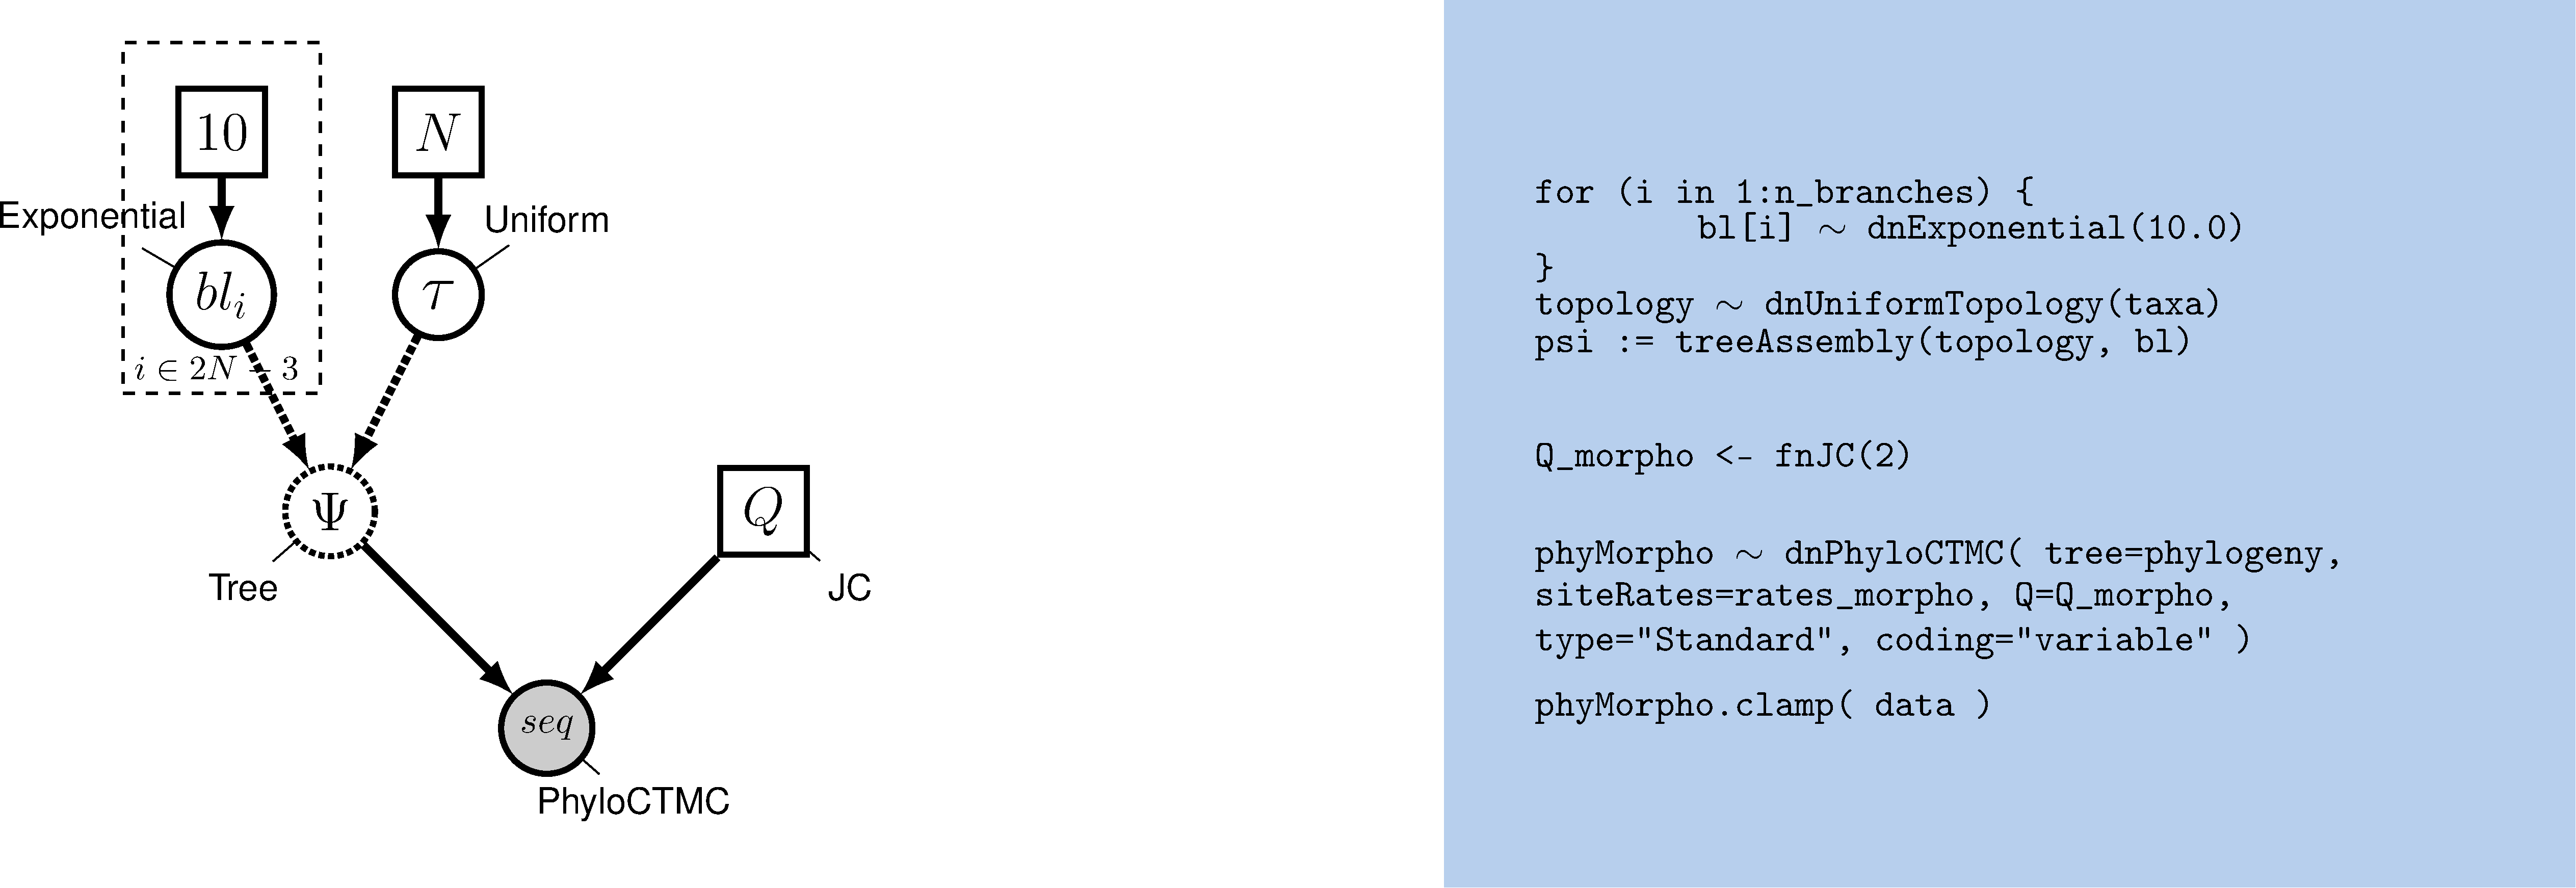
\includegraphics[width=0.92\textwidth,angle=0]{\ResourcePath figures/tikz/Mk_model}
\caption{\small Graphical model showing the Mk model (left panel). Rev code specifying the Mk model is on the right-hand panel.}
\end{minipage}}
\label{fig:module-gm}
\end{figure}
Molecular data forms the basis of most phylogenetic analyses today. 
However, morphological characters remain relevant: Fossils often provide our only direct observation of extinct biodiversity; DNA degradation can make it difficult or impossible to obtain sufficient molecular data from fragile museum specimens. 
Using morphological data can help researchers include specimens in their phylogeny that might be left out of a molecular tree. \par
To understand how morphological characters are modeled, it is important to understand how characters are collected.
Unlike in molecular data, for which homology is algorithmically determined, homology in a character is typically assessed an expert. 
Biologists will typically decide what characters are homologous by looking across specimens at the same structure in multiple taxa; they may also look at the developmental origin of structures in making this assessment \citep{Phillips06}.
Once homology is determined, characters are broken down into states, or different forms a single character can take.
The state `0' commonly refers to absence, meaning that character is not present.
In some codings, absence will mean that character has not evolved in that group.
In others, absence means that that character has not evolved in that group, and/or that that character has been lost in that group \citep{freudenstein05}. 
This type of coding is arbitrary, but both \textbf{non-random} and \textbf{meaningful}, and poses challenges for how we model the data. 
\par

Historically, most phylogenetic analyses using morphological characters have been performed using the maximum parsimony optimality criterion. 
Maximum parsimony analysis involves proposing trees from the morphological data.
Each tree is evaluated according to how many changes it implied in the data, and the tree that requires the fewest changes is preferred.
In this way of estimating a tree, a character that does not change, or changes only in one taxon, cannot be used to discriminate between trees (i.e., it does not favor a topology).
Therefore, workers with parsimony typically do not collect characters that are parsimony uninformative.
\par

In 2001, Paul Lewis \citep{lewis01} introduced a generalization of the Jukes-Cantor model of sequence evolution for use with morphological data.
This model, called the Mk (Markov model, assuming each character is in one of \textit{k} states) model provided a mathemetical formulation that could be used to estimate trees from morphological data in both likelihood and Bayesian frameworks. 
While this model is a useful step forward, as a generalization of the Jukes-Cantor, it still makes fairly simplistic assumptions.
This tutorial will guide you through estimating a phylogeny with the Mk model, and two useful extensions to the model. \par

\subsection{The Mk Model}
{\begin{framed}
Make a copy of the MCMC and model files you just made. 
Call them \cl{mcmc\_mk\_dicretized.Rev} and \cl{model\_mk\_discretized.Rev}. 
These will contain the new model parameters and models. \par 
\end{framed}}

The Mk model is a generalization of the Jukes-Cantor model of nucleotide sequence evolution, which we discussed in \textbf{Molecular Models of Character Evolution}. 
The Q matrix for a two-state Mk model looks like so:

\begin{equation*}
Q = \begin{pmatrix} -\mu_0 & \mu_{01} \\
\mu_{10} & -\mu_1  &\\
\end{pmatrix} \mbox{  ,}
\end{equation*}

This matrix can be expanded to accommodate multi-state data, as well:

\begin{equation*}
Q = \begin{pmatrix} -\mu_0 & \mu_{01} & \mu_{02} & \mu_{03} \\
\mu_{10} & -\mu_1  & \mu_{12} & \mu_{13} \\
\mu_{20} & \mu_{21} & -\mu_2  & \mu_{23} \\
\mu_{30} & \mu_{31} & \mu_{32} & -\mu_3 
\end{pmatrix} \mbox{  ,}
\end{equation*}

However, the Mk model sets transitions to be equal from any state to any other state. 
In that sense, our multistate matrix really looks like this:

\begin{equation*}
Q = \begin{pmatrix} -\mu_0 & \mu & \mu & \mu \\
\mu & -\mu_1  & \mu & \mu \\
\mu & \mu & -\mu_2  & \mu \\
\mu & \mu & \mu & -\mu_3 \\
\end{pmatrix} \mbox{  ,}
\end{equation*}

Because this is a Jukes-Cantor-like model, state frequencies do not vary as a model parameter.
These assumptions may seem unrealistic.
However, all models are a compromise between reality and generalizability.
Prior work has demonstrated that, in many conditions, the model does perform adequately \citep{wright14}.
Because morphological characters do not carry common meaning across sites in a matrix in the way that nucleotide characters do, making assumptions that fit all characters is challenging. 
A visualization of this simple model can be seen in Fig. 1.\par

We will first perform a phylogenetic analysis using the Mk model.
In further sections, we will explore how to relax key assumptions of the Mk model. \par

\subsection{Ascertainment Bias}

When Lewis first introduced the Mk model, he observed that branch lengths on the trees were greatly inflated.
The reason for this is that when morphological characters are collected, characters that do not vary, or vary in a non-parsimony-informative way (such as autapomorphies) are excluded.
Excluding these low-rate characters causes the overall amount of evolution to be over-estimated.
This causes an inflation in the branch lengths \cite{lewis01}.
\par

Therefore, when performing a morphological phylogenetic analysis, it is important to correct for this bias.
There are numerous statistically valid ways to perform this correction \cite{allman08b}.
Original corrections simulated invariant and non-parsimony informative characters along the proposed tree.
The likelihood of these characters would then be calculated and used to normalize the total likelihood value.
RevBayes implements a dynamic programming approach that calculates the same likelihood, but  does so faster. \par

\section{Example: Inferring a Phylogeny of Fossil Bears Using the Mk Model}\label{sec:dm_simple}

In this example, we will use morphological character data from 18 taxa of extinct bears \citep{abella2011}. 
The dataset contains 62 binary characters, a fairly typical dataset size for morphological characters. \par

\medskip
\subsection{Tutorial Format}\label{subsect:Exercise-Format}

This tutorial follows a specific format for issuing instructions and information.

{\begin{framed}
The boxed instructions guide you to complete tasks that are not part of the \RevBayes syntax, but rather direct you to create directories or files or similar.
\end{framed}}


Information describing the commands and instructions will be written in paragraph-form before or after they are issued.

All command-line text, including all \Rev syntax, are given in \cl{monotype font}. 
Furthermore, blocks of \Rev code that are needed to build the model, specify the analysis, or execute the run are given in separate shaded boxes.
For example, we will instruct you to create a constant node called \cl{example} that is equal to \cl{1.0} using the \cl{<-} operator like this:
%Load the cytochrome-b sequences from file and assign the data matrix to a variable called \cl{cytb}.
{\tt \begin{snugshade*}
\begin{lstlisting}
example <- 1.0
\end{lstlisting}
\end{snugshade*}
}

It is important to be aware that some PDF viewers may render some characters given as \colorbox{shadecolor}{\tt{Rev commands}} differently. 
Thus, if you copy and paste text from this PDF, you may introduce some incorrect characters. 
Because of this, we recommend that you type the instructions in this tutorial or copy them from the scripts provided. 


\medskip
\subsection{Data and Files}\label{subsect:Exercise-DataFiles}

{\begin{framed}
On your own computer, create a directory called {\textcolor{red}{\cl{RB\_DiscreteMorphology\_Tutorial}}} (or any name you like). 

In this directory download and unzip the archive containing the data files: \href{https://github.com/revbayes/revbayes_tutorial/tree/master/RB_Discrete_Morphology_Tutorial/data.zip}{\cl{data.zip}}.

This will create a folder called \cl{data} that contains the files necessary to complete this exercise.
\end{framed}}


\bigskip
\subsection{Getting Started}\label{subsect:Exercise-GetStart}

{\begin{framed}
Create a new directory (in \cl{RB\_DiscreteMorphology\_Tutorial}) called {\textcolor{red}{\cl{scripts}}}. (If you do not have this folder, please refer to the directions in section \ref{subsect:Exercise-DataFiles}.)
\end{framed}}

When you execute \RevBayes in this exercise, you will do so within the main directory you created (\cl{RB\_DiscreteMorphology\_Tutorial}), thus, if you are using a Unix-based operating system, we recommend that you add the \RevBayes binary to your path.
\bigskip

\subsection{Creating \Rev Files}\label{subsect:Exercise-CreatingFiles}

For complex models and analyses, it is best to create \Rev script files that will contain all of the model parameters, moves, and functions. 
In this exercise, you will work primarily in your text editor\footnote{In section \ref{subsub:Req-Software} we offer a recommendation for a text editor.} and create a set of modular files that will be easily managed and interchanged.
In this first section, you will write the following files from scratch and save them in the \cl{scripts} directory:
\begin{itemize}[noitemsep,topsep=0pt]
\item \cl{mcmc\_mk.Rev}: the master \Rev file that loads the data, the separate model files, and specifies the monitors and MCMC sampler.
\item \cl{model\_mk.Rev}: specifies the model describing discrete morphological character change (binary characters). 
\end{itemize}

All of the files that you will create are also provided in the \RevBayes tutorial repository\footnote{\url{https://github.com/revbayes/revbayes_tutorial/tree/master/RB_Discrete_Morphology_Tutorial/scripts}}. 
Please refer to these files to verify or troubleshoot your own scripts. 
%TODO add link to scripts

{\begin{framed}
Open your text editor and create the master \Rev file called {\textcolor{red}{\cl{mcmc\_Mk.Rev}}} in the \cl{scripts} directory.

Enter the \Rev code provided in this section in the new model file.
\end{framed}}

The file you will begin in this section will be the one you load into \RevBayes when you've completed all of the components of the analysis.
In this section you will begin the file and write the \Rev commands for loading in the taxon list and managing the data matrices.
Then, starting in section \ref{subsect:Exercise-MkModel}, you will move on to writing module files for each of the model components. 
Once the model files are complete, you will return to editing \cl{mcmc\_Mk.Rev} and complete the \Rev script with the instructions given in section \ref{subsect:Exercise-CompleteMCMC}.

\medskip
\subsubsection{Load Data Matrices}\label{subsub:Exercise-LoadData}

\RevBayes uses the function \cl{readDiscreteCharacterData()} to load a data matrix to the workspace from a formatted file. 
This function can be used for both molecular sequences and discrete morphological characters.
Import the morphological character matrix and assign it to the variable \cl{morpho}. 
{\tt \begin{snugshade*}
\begin{lstlisting}
morpho <- readDiscreteCharacterData("data/bears.nex")
\end{lstlisting}
\end{snugshade*}}

 \medskip
\subsubsection{Create Helper Variables}\label{subsub:Exercise-mviVar}

Before we begin writing the \Rev scripts for each of the model components, we need to instantiate a couple ``helper variables'' that will be used by downstream parts of our model specification files. 
These variables will be used in more than one of the module files so it's best to initialize them in the master file.

Create a new constant node called \cl{n\_taxa} that is equal to the number of species in our analysis (18). 
We will also create a constant node of the taxon names.
This list will be used to initialize the tree.

{\tt \begin{snugshade*}
\begin{lstlisting}
taxa <- morpho.names()
n_taxa <- morpho.size() 
\end{lstlisting}
\end{snugshade*}}

Next, create a workspace variable called \cl{mvi}. 
This variable is an iterator that will build a vector containing all of the MCMC moves used to propose new states for every stochastic node in the model graph. 
Each time a new move is added to the vector, \cl{mvi} will be incremented by a value of \cl{1}.
{\tt \begin{snugshade*}
\begin{lstlisting}
mvi = 1
\end{lstlisting}
\end{snugshade*}}
One important distinction here is that \cl{mvi} is part of the \RevBayes workspace and not the hierarchical model. 
Thus, we use the workspace assignment operator \cl{=} instead of the constant node assignment \cl{<-}. 

{\begin{framed}
Save your current working version of \cl{mcmc\_Mk.Rev} in the \cl{scripts} directory.

We will now move on to the next \Rev file and will complete \cl{mcmc\_Mk.Rev} in section \ref{subsect:Exercise-CompleteMCMC}.
\end{framed}}


\bigskip
\subsection{The Mk Model}

{\begin{framed}
Open your text editor and create the master \Rev file called {\textcolor{red}{\cl{model\_Mk.Rev}}} in the \cl{scripts} directory.

Enter the \Rev code provided in this section in the new model file.
\end{framed}}

First, we will create a vector of moves on branch lengths. 
This should be familiar from the \cl{RB\_CTMC} tutorial:
{\tt \begin{snugshade*}
\begin{lstlisting}
br_len_lambda ~ dnExp(0.2)
moves[mvi++] = mvScale(br_len_lambda, weight=5)
nbr <- 2*names.size() - 3
for (i in 1:nbr){
    br_lens[i] ~ dnExponential(br_len_lambda)
    moves[mvi++] = mvScale(br_lens[i]) 
}
\end{lstlisting}
\end{snugshade*}}

Next, we will create a Q matrix. 
Recall that the Mk model is simply a generalization of the JC model.
Therefore, we will create a 2x2 Q matrix using \cl{fnJC}, which initializes Q-matrices with equal transition probabilities between all states.

{\tt \begin{snugshade*}
\begin{lstlisting}
Q_morpho := fnJC(2)
\end{lstlisting}
\end{snugshade*}}

Now that we have the basics of the model specified, we will add Gamma-distributed rate variation and specify moves on the parameter to the Gamma distribution.


{\tt \begin{snugshade*}
\begin{lstlisting}
alpha_morpho ~ dnExponential( 1.0 )
rates_morpho := fnDiscretizeGamma( alpha_morpho, alpha_morpho, 4 )

#Moves on the parameters to the Gamma distribution.
moves[mvi++] = mvScale(alpha_morpho, lambda=0.01, weight=5.0)
moves[mvi++] = mvScale(alpha_morpho, lambda=0.1,  weight=3.0)
moves[mvi++] = mvScale(alpha_morpho, lambda=1,    weight=1.0)
\end{lstlisting}
\end{snugshade*}}

Next we assemble the tree and specify a move on the topology.

{\tt \begin{snugshade*}
\begin{lstlisting}
tau ~ dnUniformTopology(names)
phylogeny := treeAssembly(tau, br_lens)
moves[mvi++] = mvNNI(tau, weight=2*nbr)
moves[mvi++] = mvSPR(tau, weight=nbr)
tree_length := phylogeny.treeLength()
\end{lstlisting}
\end{snugshade*}}

Lastly, we set up the CTMC. 
This should be familiar from the \cl{RB\_CTMC} tutorial.
We see some familiar pieces: tree, Q matrix and site\_rates.
We also have two new keywords: data type and coding.
The data type argument specifies the type of data - in our case, "Standard", the specification for morphology.
Coding specifies what type of ascertainment bias is expected.
We are using the `variable' correction, as we have no invariant character in our matrix.
If we also lacked parsimony non-informative characters, we would use the coding `informative'. 

{\tt \begin{snugshade*}
\begin{lstlisting}
phyMorpho ~ dnPhyloCTMC(tree=phylogeny, siteRates=rates_morpho, Q=Q_morpho, type="Standard", coding="variable")
phyMorpho.clamp(morpho)
\end{lstlisting}
\end{snugshade*}}

All of the components of the model are now specified. \par

\subsection{Complete Master \Rev File}\label{subsect:Exercise-CompleteMCMC}

{\begin{framed}
Return to the master \Rev file you created in section \ref{subsect:Exercise-StartMasterRev} called {\textcolor{red}{\cl{mcmc\_Mk.Rev}}} in the \cl{scripts} directory.

Enter the \Rev code provided in this section in this file.
\end{framed}}

\medskip
\subsubsection{Source Model Scripts}\label{subsub:Exercise-SourceMods}

\RevBayes uses the \cl{source()} function to load commands from \Rev files into the workspace.
Use this function to load in the model scripts we have written in the text editor and saved in the \cl{scripts} directory.
{\tt \begin{snugshade*}
\begin{lstlisting}
source("scripts/model_Mk.Rev")

\end{lstlisting}
\end{snugshade*}}


\medskip
\subsubsection{Create Model Object}\label{subsub:Exercise-ModObj}

We can now create our workspace model variable with our fully specified model DAG. 
We will do this with the \cl{model()} function and provide a single node in the graph (\cl{phylogeny}).
{\tt \begin{snugshade*}
\begin{lstlisting}
mymodel = model(phylogeny)
\end{lstlisting}
\end{snugshade*}}

The object \cl{mymodel} is a wrapper around the entire model graph and allows us to pass the model to various functions that are specific to our MCMC analysis.

\medskip
\subsubsection{Specify Monitors and Output Filenames}\label{subsub:Exercise-Monitors}

The next important step for our master \Rev file is to specify the monitors and output file names.
For this, we create a vector called \cl{monitors} that will each sample and record or output our MCMC. 

First, we will specify a workspace variable to iterate over the \cl{monitors} vector.
{\tt \begin{snugshade*}
\begin{lstlisting}
mni = 1
\end{lstlisting}
\end{snugshade*}}

The first monitor we will create will monitor every named random variable in our model graph. 
This will include every stochastic and deterministic node using the \cl{mnModel} monitor.
The only parameter that is not included in the \cl{mnModel} is the tree topology. 
Therefore, the parameters in the file written by this monitor are all numerical parameters written to a tab-separated text file that can be opened by accessory programs for evaluating such parameters.
We will also name the output file for this monitor and indicate that we wish to sample our MCMC every 10 cycles.
{\tt \begin{snugshade*}
\begin{lstlisting}
monitors[mni++] = mnModel(filename="output/mk_simple.log", printgen=10)
\end{lstlisting}
\end{snugshade*}}

The \cl{mnFile} monitor writes any parameter we specify to file.
Thus, if we only cared about the branch lengths and nothing else (this is not a typical or recommended attitude for an analysis this complex) we wouldn't use the \cl{mnModel} monitor above and just use the \cl{mnFile} monitor to write a smaller and simpler output file.
Since the tree topology is not included in the \cl{mnModel} monitor (because it is not numerical), we will use \cl{mnFile} to write the tree to file by specifying our \cl{phylogeny} variable in the arguments.
{\tt \begin{snugshade*}
\begin{lstlisting}
monitors[mni++] = mnFile(filename="output/mk_simple.trees", printgen=10, phylogeny)
\end{lstlisting}
\end{snugshade*}}

The third monitor we will add to our analysis will print information to the screen.
Like with \cl{mnFile} we must tell \cl{mnScreen} which parameters we'd like to see updated on the screen. 
{\tt \begin{snugshade*}
\begin{lstlisting}
monitors[mni++] = mnScreen(printgen=10)
\end{lstlisting}
\end{snugshade*}}

Finally, we'll create an ancestral state monitor, which is described in more detail in Section \ref{sec:anc_states}.
{\tt \begin{snugshade*}
\begin{lstlisting}
monitors[mni++] = mnJointConditionalAncestralState(
    tree=phylogeny,
    ctmc=phyMorpho,
    filename="output/mk_simple.states.txt",
    type="Standard",
    printgen=10,
    withStartStates=false)
\end{lstlisting}
\end{snugshade*}}


\medskip
\subsubsection{Set-Up the MCMC}

Once we have set up our model, moves, and monitors, we can now create the workspace variable that defines our MCMC run. 
We do this using the \cl{mcmc()} function that simply takes the three main analysis components as arguments.
{\tt \begin{snugshade*}
\begin{lstlisting}
mymcmc = mcmc(mymodel, monitors, moves)\end{lstlisting}
\end{snugshade*}}

The MCMC object that we named \cl{mymcmc} has a member method called \cl{.run()}. 
This will execute our analysis and we will set the chain length to \cl{10000} cycles using the \cl{generations} option.
{\tt \begin{snugshade*}
\begin{lstlisting}
mymcmc.run(generations=20000)
\end{lstlisting}
\end{snugshade*}}

Once our Markov chain has terminated, we will want \RevBayes to close. 
Tell the program to quit using the \cl{q()} function.
{\tt \begin{snugshade*}
\begin{lstlisting}
q()
\end{lstlisting}
\end{snugshade*}}

{\begin{framed}
You made it! Save all of your files.
\end{framed}}

\bigskip
\subsection{Execute the MCMC Analysis}\label{subsect:Exercise-RunMCMC}

With all the parameters specified and all analysis components in place, you are now ready to run your analysis. 
The \Rev scripts you just created will all be used by \RevBayes and loaded in the appropriate order.

{\begin{framed}
Begin by running the \RevBayes executable. In Unix systems, type the following in your terminal (if the \RevBayes binary is in your path):

\colorbox{black}{\strut\hspace{1mm}\textcolor[rgb]{0,1,1}{\cl{rb}}\hspace{0.925\textwidth}}
\end{framed}}

Provided that you started \RevBayes from the correct directory (\cl{RB\_DiscreteMorphology\_Tutorial}), you can then use the \cl{source()} function to feed \RevBayes your master script file (\cl{mcmc\_mk.Rev}).
{\tt \begin{snugshade*}
\begin{lstlisting}
source("scripts/mcmc_mk.Rev")
\end{lstlisting}
\end{snugshade*}}

This will execute the analysis and you should see the following output (though not the exact same values):


{\tiny{\tt \begin{snugshade*}
\begin{lstlisting}
|* source("scripts/mcmc_mk.rev")
|*   Processing file "scripts/mcmc_mk.rev"
|*   Successfully read one character matrix from
|* file 'data/bears.nex'
|*   Processing file "scripts/mk_simple.rev"
|*   Processing of file "scripts/mk_simple.rev"
|* completed

|*   Running MCMC simulation
|*   This simulation runs 1 independent replicate.
|*   The simulator uses 37 different moves in a
|* random move schedule with 37 moves per iteration
|*
|* Iter        |      Posterior   |     Likelihood  
|* |          Prior   |    elapsed   |        ETA   
|*
|*
|* ---------------------------------------------------------------------------------------------------
|* 0           |       -685.779   |       -666.105   |       -19.6731   |   00:00:00   |   --:--:--   |

|* 10          |       -633.737   |       -608.951   |        -24.786   |   00:00:00   |   --:--:--   |

|* 20          |       -593.634   |       -558.797   |       -34.8368   |   00:00:00   |   00:00:00   |
|* 30          |       -578.661   |       -536.125   |       -42.5362   |   00:00:00   |   00:00:00   |
|* 40          |        -544.22   |       -514.098   |       -30.1223   |   00:00:00   |   00:00:00   |
|* 50          |       -515.505   |       -492.988   |       -22.5169   |   00:00:00   |   00:00:00   |
|* 60          |       -483.695   |       -461.347   |       -22.3479   |   00:00:00   |   00:00:00   |

|*...
\end{lstlisting}
\end{snugshade*}}}

When the analysis is complete, \RevBayes will quit and you will have a new directory called \cl{output} that will contain all of the files you specified with the monitors (Sect.\ \ref{subsub:Exercise-Monitors}).

\subsubsection{Ascertainment Bias}

As discussed in (Sect.\ \ref{subsub:Ascertainment Bias}), we also need to correct for ascertainment bias. 
Once your initial Mk model estimation, source the mcmc\_simple.Rev script. 
This file is an estimation of the Mk model without any correction for ascertainment bias. 
We will use this for comparison in a moment. \par


 

\newpage

\section{Beyond binary rate matrices} \label{sec:dm_matrix}

The instantaneous rate matrix encodes the transition rates between all pairs of evolutionary states.
It is important to emphasize that all rate matrices are assertions about how morphological evolution operates.
Depending on how one populates the rate matrix elements, different evolutionary hypotheses may be expressed. \par

When we model the evolution of morphological data, unlike nucleotide data, each change may require a sequence of intermediate changes.
Getting to one state may require going through another.
In short, it is probably not likely that one single model describes all characters well. \par 


\subsection{Symmetric unordered}

The standard Mk model of character evolution, where M denotes it is a Markov model and $K$ denotes the number of states for the character.
The lineage may transition directly from state 1 to state 4 without going through states 2 and 3, which is representative of a character with {\it unordered} states.
In addition, all transition rates are equal as they are in the Jukes-Cantor rate matrix \citep{jukes69}.
Here is an example of a symmetric unordered Mk model for $K=4$.

\begin{equation*}
Q = \begin{pmatrix}
- & r & r & r \\
r & - & r & r \\
r & r & - & r \\
r & r & r & - 
\end{pmatrix}
\end{equation*}


Define the single shared rate parameter
{\tt \begin{snugshade*}
\begin{lstlisting}
r <- 1.0
\end{lstlisting}
\end{snugshade*}}

Define the rates
{\tt \begin{snugshade*}
\begin{lstlisting}
rates := [ [0.0,   r,   r,   r],
           [  r, 0.0,   r,   r],
           [  r,   r, 0.0,   r],
           [  r,   r,   r, 0.0] ]
\end{lstlisting}
\end{snugshade*}}

Create the rate matrix
{\tt \begin{snugshade*}
\begin{lstlisting}
Q := fnFreeK(rates)
Q
|*[ [ -1.0000, 0.3333, 0.3333, 0.3333 ] ,
|*    0.3333, -1.0000, 0.3333, 0.3333 ] ,
|*    0.3333, 0.3333, -1.0000, 0.3333 ] ,
|*    0.3333, 0.3333, 0.3333, -1.0000 ] ]
\end{lstlisting}
\end{snugshade*}}

Compute the transition probability matrix for a branch length of 0.1.

{\tt \begin{snugshade*}
\begin{lstlisting}
P <- Q.getTransitionProbabilities(0.1)
P
|*[ [ 0.906, 0.031, 0.031, 0.031],
|*  [ 0.031, 0.906, 0.031, 0.031],
|*  [ 0.031, 0.031, 0.906, 0.031],
|*  [ 0.031, 0.031, 0.031, 0.906] ]
\end{lstlisting}
\end{snugshade*}}

If we believed that, for example, for a couple of states, some transitions are strongly more likely, we could add a multiplier between those two states:

{\tt \begin{snugshade*}
\begin{lstlisting}
rates := [ [0.0,   r*2,   r,   r],
           [  r, 0.0,   r,   r],
           [  r,   r, 0.0,   r],
           [  r,   r*2,   r, 0.0] ]
Q := fnFreeK(rates)
Q
   [ [ -1.1765, 0.5882, 0.2941, 0.2941 ] ,
     0.2941, -0.8824, 0.2941, 0.2941 ] ,
     0.2941, 0.2941, -0.8824, 0.2941 ] ,
     0.2941, 0.5882, 0.2941, -1.1765 ] ]

 P <- Q.getTransitionProbabilities(0.1)
 P
   [ [ 0.891, 0.054, 0.028, 0.027], 
   [ 0.027, 0.918, 0.028, 0.027], 
   [ 0.027, 0.029, 0.917, 0.027], 
   [ 0.027, 0.054, 0.028, 0.891]]
\end{lstlisting}
\end{snugshade*}}

If we then get our transition probabilities, we see that this changes our probability of observing the not simply of our two state transitions that we changed the rate for, but others as well.

This type of approach is common in parsimony, where it is one of several things referred to as weighted parsimony. 
This approach to using different matrices requires you to, \textit{a priori} specify your matrix.
But in reality, there is often fairly little guidance or information by which we decide if a weight applied to a transition is appropriate.
Biologists still use models of this type - the Dollo model, in which a character is assumed not to be able to re-evolve once lost, is an extreme version of penalizing one change.

Because the transition rates between all differing pairs of states are the same, so are the transition probabilities.
Similarly, the probability of remaining in any given state is also equal across states.

\subsection{Asymmetric ordered}

Character states that are ordered imply that evolutionary transitions occur in particular sequences.
For example, the number of digits on a foot might vary by gaining and losing single digits, meaning the transition from three to five digits cannot occur without going through the evolutionary state of possessing four digits.
Below, we assume that gain events ( $n \rightarrow n+1$ ) occur at rate $\mu_1$ and loss events ($n \rightarrow n-1$) occur at rate $\mu_2$.
The zeroes indicate that there is no immediate evolutionary path between states $1$ and $4$: states $2$ and $3$ must be used to reach $4$ from $1$.

\begin{equation*}
Q = \begin{pmatrix}
- & r_1 & 0 & 0 \\
r_2 & -   & r_1 & 0 \\
0 & r_2 & -   & r_1 \\
0 & 0 & r_2 & - 
\end{pmatrix}
\end{equation*}


Create a simplex of unscaled rate parameters for gain ({\tt r[1]}) and loss ({\tt r[2]}) events.
The simplex is assigned a flat Dirichlet prior with an initial gain-to-loss rate ratio of 3:1

{\tt \begin{snugshade*}
\begin{lstlisting}
r ~ dnDirichlet( [1,1] )
r.setValue( simplex(3,1) )
\end{lstlisting}
\end{snugshade*}}

Create a tridiagonal matrix of transition rates, meaning state $i$ may only transition to states $i-1$ and $i+1$

{\tt \begin{snugshade*}
\begin{lstlisting}
rates := [ [  0.0, r[1],  0.0,  0.0],
           [ r[2],  0.0, r[1],  0.0],
           [  0.0, r[2],  0.0, r[1]],
           [  0.0,  0.0, r[2],  0.0] ]
\end{lstlisting}
\end{snugshade*}}

Create the rate matrix

{\tt \begin{snugshade*}
\begin{lstlisting}
Q := fnFreeK(rates)
|*[ [ -1.5385, 1.5385, 0.0000, 0.0000 ] ,
|*     0.5128, -2.0513, 1.5385, 0.0000 ] ,
|*     0.0000, 0.5128, -2.0513, 1.5385 ] ,
|*     0.0000, 0.0000, 0.5128, -0.5128 ] ]
\end{lstlisting}
\end{snugshade*}}

Compute the transition probability matrix for a branch length of 0.1.

{\tt \begin{snugshade*}
\begin{lstlisting}
P <- Q.getTransitionProbabilities(rate=0.1)
|*[ [ 0.861, 0.129, 0.010, 0.001],
|*  [ 0.043, 0.821, 0.126, 0.010],
|*  [ 0.001, 0.042, 0.821, 0.136],
|*  [ 0.000, 0.001, 0.045, 0.954]]
\end{lstlisting}
\end{snugshade*}}

Note that {\tt P[1][2]} > {\tt P[1][3]} > {\tt P[1][4]}, primarily because those transitions require a minimum of one, two, and three events, respectively.
In addition, note that assigning asymmetric transition rates causes {\tt P[1][2]} > {\tt P[2][1]} because {\tt rates[1][2]} > {\tt rates[2][1]}.


\subsection{Correlated binary characters}

Two characters do not necessarily evolve independently of one another.
Take two characters in plants: the presence or absence of toothed leaf margins (character X) is thought to be ecologically correlated with the presence of absence of leaf lobing (character Y).
For a single binary character, there are two states (0 and 1), but there are four states for a pair of non-independent binary characters (00, 10, 01, and 11).
\citet{pagel04} introduced a general framework for modeling the evolution of joint sets of characters.
These models require that only one evolutionary event can occur in a moment of time, which is enforced with the 0 terms.
In addition, the transition rate that, say, character X goes from 0 to 1 depends on the current value of character Y.

\subsubsection{Seven free parameters}

In the first case, all possible transitions might be assigned their own parameter.
Here, we'll assign a simplex over all rates, leaving seven free parameters (plus an eighth parameter that scales the rate matrix).

\begin{equation*}
Q = \begin{pmatrix}
                      - & \mu_{00 \rightarrow 10} & \mu_{00 \rightarrow 01} &                       0 \\
\mu_{10 \rightarrow 00} &                       - &                       0 & \mu_{10 \rightarrow 11} \\
\mu_{01 \rightarrow 00} &                       0 &                       - & \mu_{01 \rightarrow 11} \\
                      0 & \mu_{11 \rightarrow 10} & \mu_{11 \rightarrow 01} &                       - \\
\end{pmatrix}
\end{equation*}

{\tt \begin{snugshade*}
\begin{lstlisting}
r ~ dnDirichlet( [1,1,1,1,1,1,1,1] )
r.setValue( simplex(1,1,3,3,3,3,1,1) )
\end{lstlisting}
\end{snugshade*}}

Create an array of zeroes for the four states (00, 10, 01, 11)

{\tt \begin{snugshade*}
\begin{lstlisting}
for (i in 1:4) {
    for (j in 1:4) {
        rates[i][j] <- 0.0
    }
}
\end{lstlisting}
\end{snugshade*}}

Populate the elements of {\tt rates}

{\tt \begin{snugshade*}
\begin{lstlisting}
rates[1][2] := r[1] # 00->10
rates[1][3] := r[2] # 00->01
rates[2][1] := r[3] # 10->00
rates[2][4] := r[4] # 10->11
rates[3][1] := r[5] # 01->00
rates[3][4] := r[6] # 01->11
rates[4][2] := r[7] # 11->10
rates[4][3] := r[8] # 11->01
\end{lstlisting}
\end{snugshade*}}

Create the rate matrix

{\tt \begin{snugshade*}
\begin{lstlisting}
Q := fnFreeK(rates)
|*[ [ -0.6667, 0.3333, 0.3333, 0.0000 ] ,
|*     1.0000, -2.0000, 0.0000, 1.0000 ] ,
|*     1.0000, 0.0000, -2.0000, 1.0000 ] ,
|*     0.0000, 0.3333, 0.3333, -0.6667 ] ]
\end{lstlisting}
\end{snugshade*}}

Compute the transition probability matrix for a branch length of 0.1.

{\tt \begin{snugshade*}
\begin{lstlisting}
P <- Q.getTransitionProbabilities(rate=0.1)
|*[ [ 0.938, 0.029, 0.029, 0.003],
|*  [ 0.088, 0.822, 0.003, 0.088],
|*  [ 0.088, 0.003, 0.822, 0.088],
|*  [ 0.003, 0.029, 0.029, 0.938] ]
\end{lstlisting}
\end{snugshade*}}

Note that the probability of remaining in state 10 or state 01 is less than the probability of remaining in state 00 or state 11.
In this toy example, these probabilities reflect that states 10 an 01 are less evolutionarily stable than states 00 and 11.

\subsubsection{Four free parameters}

Alternatively, characters X and Y might share state frequencies, $\pi_j$, and transition rates $\mu_{ij}^{(k)}$, where $i$ is the starting state for the character undergoing change, $j$ is the ending state, and $k$ is the state of the other character.
This results in two stationary frequencies (one free parameter), four transition rates for $0 \rightarrow 1$ and $1 \rightarrow 0$ given that the other character is in state 0 or state 1 (three free parameters), plus one free parameter to scale the rate matrix.

\begin{equation*}
Q = \begin{pmatrix}
- & \mu_{01}^{(0)} \pi_1 \pi_0 & \mu_{01}^{(0)} \pi_0 \pi_1 & 0 \\
\mu_{10}^{(0)} \pi_0 \pi_0 & -   & 0 & \mu_{01}^{(1)} \pi_1 \pi_1 \\
\mu_{10}^{(0)} \pi_0 \pi_0 & 0   & - & \mu_{01}^{(1)} \pi_1 \pi_1 \\
0 & \mu_{10}^{(1)} \pi_1 \pi_0 & \mu_{10}^{(1)} \pi_0 \pi_1 & - \\
\end{pmatrix}
\end{equation*}

Assign the stationary frequencies of being in state 0 or state 1 shared by both characters X and Y.

{\tt \begin{snugshade*}
\begin{lstlisting}
pi ~ dnDirichlet([1,1])
pi.setValue( simplex(1,3) )
\end{lstlisting}
\end{snugshade*}}

Assign the relative transition rates for gain and loss provided that the other character is in state 0 or 1.

{\tt \begin{snugshade*}
\begin{lstlisting}
r ~ dnDirichlet( [1,1,1,1] )
r.setValue( simplex(1,3,3,1) )
\end{lstlisting}
\end{snugshade*}}

Create an array of zeroes for the four states (00, 10, 01, 11)

{\tt \begin{snugshade*}
\begin{lstlisting}
for (i in 1:4) {
    for (j in 1:4) {
        rates[i][j] <- 0.0
    }
}
\end{lstlisting}
\end{snugshade*}}

Populate the elements of {\tt rates}

{\tt \begin{snugshade*}
\begin{lstlisting}
rates[1][2] := r[1] * pi[2] * pi[1] # 00->10
rates[1][3] := r[1] * pi[1] * pi[2] # 00->01
rates[2][1] := r[3] * pi[1] * pi[1] # 10->00
rates[2][4] := r[2] * pi[2] * pi[2] # 10->11
rates[3][1] := r[2] * pi[1] * pi[1] # 01->00
rates[3][4] := r[3] * pi[2] * pi[2] # 01->11
rates[4][2] := r[4] * pi[2] * pi[1] # 11->10
rates[4][3] := r[4] * pi[1] * pi[2] # 11->01
\end{lstlisting}
\end{snugshade*}}

Create the rate matrix

{\tt \begin{snugshade*}
\begin{lstlisting}
Q := fnFreeK(rates)
Q
|*[ [ -0.6333, 0.3167, 0.3167, 0.0000 ] ,
|*     0.4750, -2.3750, 0.0000, 1.9000 ] ,
|*     0.4750, 0.0000, -2.3750, 1.9000 ] ,
|*     0.0000, 0.3167, 0.3167, -0.6333 ] ]
\end{lstlisting}
\end{snugshade*}}

Compute the transition probability matrix for a branch length of 0.1.

{\tt \begin{snugshade*}
\begin{lstlisting}
P <- Q.getTransitionProbabilities(0.1)
P
|*[ [ 0.940, 0.027, 0.027, 0.005],
|*  [ 0.041, 0.792, 0.003, 0.164],
|*  [ 0.041, 0.003, 0.792, 0.164],
|*  [ 0.001, 0.027, 0.027, 0.944] ]
\end{lstlisting}
\end{snugshade*}}

Note that this model has a tendency towards state 11.

{\tt \begin{snugshade*}
\begin{lstlisting}
P_10 <- Q.getTransitionProbabilities(10.0)
P_10
|*[ [ 0.159, 0.105, 0.105, 0.630],
|*  [ 0.158, 0.105, 0.105, 0.632],
|*  [ 0.158, 0.105, 0.105, 0.632],
|*  [ 0.158, 0.105, 0.105, 0.632] ]
\end{lstlisting}
\end{snugshade*}}


\subsection{Covarion}

Covarion models \citep{tuffley98} capture the possibility that a ``hidden'' (unobserved or unmeasurable) states cause evolutionary processes to vary in tempo and modes.
For example, phylogenetically local clusters of plant lineages appear to transition between herbaceous and woody habits at relatively high rates, so one might want to quantify where these bursts occur \citep{beaulieu2013}.
While similar in structure to the correlated character model of \citet{pagel94}, covarion models do not observe the hidden state that induce the mode-shifts.
Instead, covarion models expand the character's state space by a factor of $K$, and observe the character once for each of the $K$ categories.
For example, take a binary character modeled with $K=2$ hidden state classes.
The model would treat a character that is observed as being in state 0 as possibly being in either of the $K=2$ classes (0,1) and (0,2).
In practice, this is done by setting the likelihood of observing those $0k$ states to equal 1.

The expanded structure of a simple covarion rate matrix with $K=2$ is

\begin{equation*}
Q = \left(
\arraycolsep=6pt\def\arraystretch{2.5}
\begin{array}{cc|cc}
- & r_1 q_{01}^{(1)} & s_{12} & 0 \\
r_1 q_{10}^{(1)} & - & 0 & s_{12} \\
\hline
s_{21} & 0 & - & r_2 q_{01}^{(2)} \\
0 & s_{21} & r_2 q_{10}^{(2)} & -  \\

\end{array}
\right)    
\end{equation*}

This form can be reduced to a simpler block-matrix representation

\begin{equation*}
Q = \left(
\arraycolsep=8pt\def\arraystretch{3.0}
\begin{array}{c|c}
r_1 Q^{(1)} & s_{12} I  \\
\hline
s_{21} I & r_2 Q^{(2)} \\
\end{array}
\right)
\end{equation*}


where $Q^{(i)}$ is the rate matrix for the $i$th class, $r_i \in r$ is the clock rate for the $i$th class, and $S$ is the rate matrix to switch between classes.


{\tt \begin{snugshade*}
\begin{lstlisting}
sr ~ dnDirichlet([1,1])
sr.setValue( simplex(1,2) )
switch_rates := [ [   0.0, sr[1] ],
                  [ sr[2],   0.0 ] ]
Q_switch := fnFreeK(switch_rates)
\end{lstlisting}
\end{snugshade*}}

Create an array of zeroes for the four states (00, 10, 01, 11)

{\tt \begin{snugshade*}
\begin{lstlisting}
cr[1] ~ dnExp(1)
cr[2] ~ dnExp(1)
cr[1].setValue(3)
cr[2].setValue(1)
\end{lstlisting}
\end{snugshade*}}

Populate the elements of {\tt rates}

{\tt \begin{snugshade*}
\begin{lstlisting}
Q_class[1] := fnJC(2)

bf ~ dnDirichlet( [1,1] )
bf.setValue( simplex(1,3) )
Q_class[2] := fnF81( bf )

\end{lstlisting}
\end{snugshade*}}

Create the rate matrix

{\tt \begin{snugshade*}
\begin{lstlisting}
Q := fnCovarionRateMatrix(Q=Q_class, switch_rates=Q_switch, clock_rates=cr)

Q
|*[ [ -1.1126, 0.8901, 0.2225, 0.0000 ] ,
|*     0.8901, -1.1126, 0.0000, 0.2225 ] ,
|*     0.4451, 0.0000, -1.0385, 0.5934 ] ,
|*     0.0000, 0.4451, 0.1978, -0.6429 ] ]
\end{lstlisting}
\end{snugshade*}}

Compute the transition probability matrix for a branch length of 0.1.

{\tt \begin{snugshade*}
\begin{lstlisting}
P <- Q.getTransitionProbabilities(0.1)
P <- Q.getTransitionProbabilities(1)
P
|*[ [ 0.899, 0.080, 0.020, 0.002],
|*  [ 0.080, 0.899, 0.001, 0.020],
|*  [ 0.040, 0.003, 0.902, 0.055],
|*  [ 0.002, 0.041, 0.018, 0.939] ]
\end{lstlisting}
\end{snugshade*}}

The rows and columns correspond to (in order): state 0 evolving by $r_1 Q^{(1)}$, state 1 evolving by $r_1 Q^{(1)}$, state 1 evolving by $r_2 Q^{(2)}$, and state 2 evolving by $r_2 Q^{(2)}$.
Note that {\tt P[1][2]} > {\tt P[3][4]}, which is largely due to the fact that $r_1 > r_2$.

\newpage

\section{Example: Relaxing the Assumption of Equal Transition Probabilities }\label{sec:dm_disc}


{\begin{framed}
Make a copy of the MCMC and model files you just made. 
Call them \cl{mcmc\_mk\_dicretized.Rev} and \cl{model\_mk\_discretized.Rev}. 
These will contain the new model parameters and models. \par 
\end{framed}}
\begin{figure}[h!]
\fbox{%
\begin{minipage}{\textwidth}\centering
% \includegraphics[width=0.5\textwidth,angle=0]{\ResourcePath figures/tikz/morpho_gm-eps-converted-to} % 
\caption{\small Graphical model demonstrating the discretized Beta distribution for allowing variable state frequencies.}
\end{minipage}}
\label{fig:module-gm}
\end{figure}
The Mk model makes a number of assumptions, but one that may strike you as unrealistic is the assumption that characters are equally likely to change from any one state to any other state.
That means that a trait is as likely to be gained as lost.
While this may hold true for some traits, we expect that it may be untrue for many others. \par
\cl{RevBayes} has functionality to allow us to relax this assumption.
We do this by specifying a Beta prior on state frequencies.
Remember from the \cl{RB\_CTMC} lesson that stationary frequencies impact how likely we are to see changes in a character.
For example, it may be very likely, in a character, to change from 0 to 1.
But if the frequency of 0 is very low, we will still seldom see this change. \par
We can exploit the relationship between state frequencies and observed changes to allow for variable Q matrices across characters (Fig. 2).
To do this, we generate a Beta distribution on state frequencies \citep{huelsenbeck01c}, and use the state frequencies from that Beta distribution to generate a series of Q-matrices to use to evaluate our data \citep{pagel04}. \par
This type of model is called a \textbf{mixture model}.
There are assumed to be subdivisions in the data, which may require different parameters (in this case, state frequencies).
These subdivisions are not defined \textit{a priori}. 
This model has previously been shown to be effective for a range of empirical and simulated datasets \citep{wright16}.\par




\subsection{Modifying the MCMC File}

At each place in which the output files are specified in the MCMC file, change the output path so you don't overwrite the output from the previous exercise. 
For example, you might call your output file \cl{output/mk\_discretized.log} and \cl{output/mk\_discretized.trees}.
Change source statement to indicate the new model file.

\subsection{Modifying the Model File}

Open the new model file that you created. We need to modify the way in which the Q matrix is specified. 
We will use a discretized Beta distribution to place a prior on state frequencies. 
The Beta distribution has two parameters, $\alpha$ and $\beta$.
These two parameters specify the shape of the distribution.
State frequencies will be evaluated according to this distribution, in the same way that rate variation is evaluated according to the Gamma distribution. 
The discretized distribution is split into multiple classes, each with it's own set of frequencies for the 0 and 1 characters.
The number of classes can vary; we have chosen 4 for tractability.\par

{\tt \begin{snugshade*}
\begin{lstlisting}
n_cats = 4
alpha_ofbeta ~ dnExponential( 1 )
beta_ofbeta ~ dnExponential( 1 )
moves[mvi++] = mvScale(alpha_ofbeta, lambda=1,    weight=1.0 )
moves[mvi++] = mvScale(alpha_ofbeta, lambda=0.1,  weight=3.0 )
moves[mvi++] = mvScale(alpha_ofbeta, lambda=0.01, weight=5.0 )
moves[mvi++] = mvScale(beta_ofbeta, lambda=1,    weight=1.0 )
moves[mvi++] = mvScale(beta_ofbeta, lambda=0.1,  weight=3.0 )
moves[mvi++] = mvScale(beta_ofbeta, lambda=0.01, weight=5.0 )
\end{lstlisting}
\end{snugshade*}}

Above, we initialized the number of categories,  the parameters to the Beta distribution, and the moves on the parameters to the Beta. 

Next, we set the categories to each represent a quadrant of the Beta distribution specified by the \cl{alpha\_ofbeta} and \cl{beta\_ofbeta}. The {\tt +1} values are added to the beta shape and scale parameters to prevent model overfitting.

{\tt \begin{snugshade*}
\begin{lstlisting}
cats := fnDiscretizeBeta(alpha_ofbeta+1, beta_ofbeta+1, 4)
\end{lstlisting}
\end{snugshade*}}

If you were to print the \cl{cats} variable, you would see a list of state frequencies like so:

{\tiny{\tt \begin{snugshade*}
\begin{lstlisting}
|*   0.0780943
|*   0.40457
|*   0.769453
|*   0.97106
\end{lstlisting}
\end{snugshade*}}}

Using these state frequencies, we will generate a new vector of Q matrices.
Because we are varying the state frequencies, we must use a Q matrix generation function that allows for state frequencies to vary as a parameter.
We will, therefore, use the \cl{fnF81} function.

{\tt \begin{snugshade*}
\begin{lstlisting}
for (i in 1:cats.size())
{
    Q[i] := fnF81(simplex(abs(1-cats[i]), cats[i]))
}
\end{lstlisting}
\end{snugshade*}}

Once we've made the our vector of matrices, we specified moves on our matrix vector:
{\tt \begin{snugshade*}
\begin{lstlisting}
matrix_probs ~ dnDirichlet(v(1,1,1,1))
moves[mvi++] = mvSimplexElementScale(matrix_probs, alpha=10, weight=1.0) 
\end{lstlisting}
\end{snugshade*}}

This Dirichlet prior says that no category is expected to have more characters than another. If you expected some category to hold more of the characters, you could put more weight on that category. \par

The only other specification that needs to change in the model file is the CTMC:
{\tt \begin{snugshade*}
\begin{lstlisting}
phyMorpho ~ dnPhyloCTMC(tree=phylogeny, siteRates=rates_morpho, Q=Q, type="Standard", coding="variable", siteMatrices=matrix_probs)
\end{lstlisting}
\end{snugshade*}}

You'll notice that we've added a command to tell the CTMC that we have multiple site matrices that will be applied to different characters in the matrix.

\medskip
\subsubsection{Set-Up the MCMC}

The MCMC chain set-up does not need to change. 
Run the new MCMC file, just as you ran the plain Mk file.
This estimation will take longer than the Mk model, due to increased model complexity. \par


\section{Site-Heterogeneous Discrete Morphology Model} \label{sec:dm_dir}

\begin{figure}[h!]
\fbox{%
\begin{minipage}{\textwidth}\centering
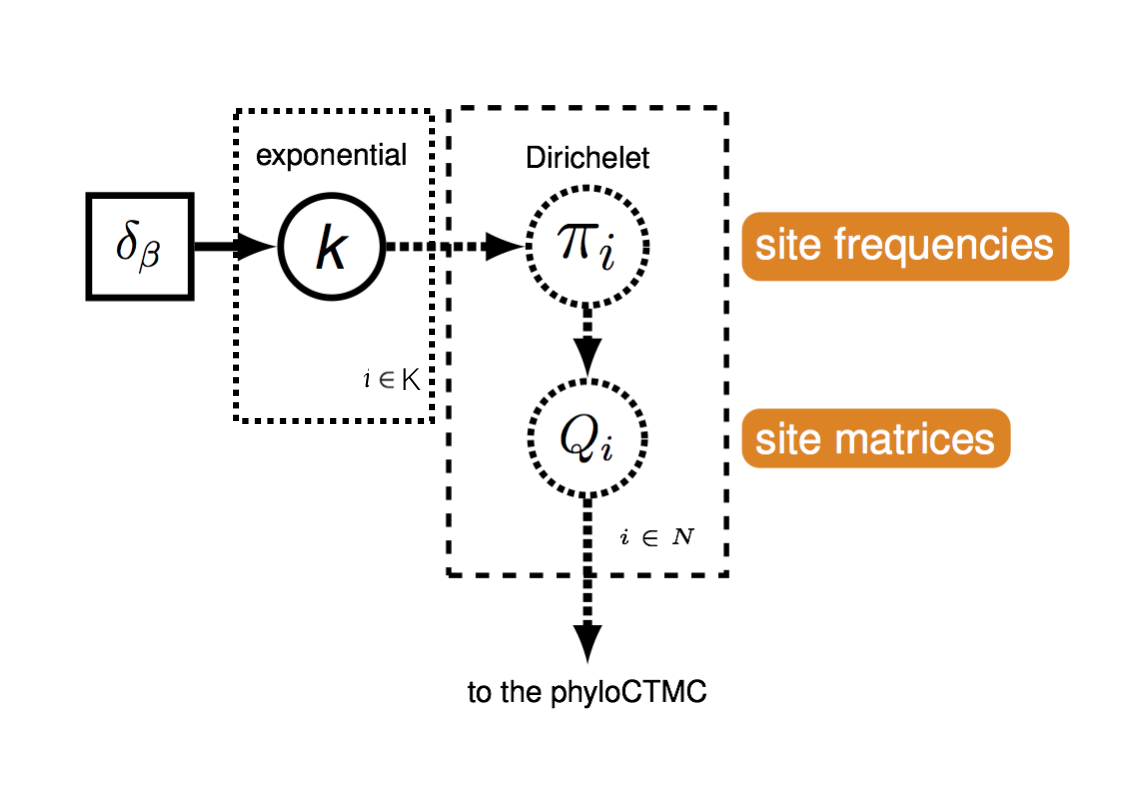
\includegraphics[width=0.5\textwidth,angle=0]{\ResourcePath figures/catplate}
\caption{\small Graphical model demonstrating the Dirichlet prior to allow variable state frequencies in both binary and multistate data.}
\end{minipage}}
\label{fig:module-relaxed morphology}
\end{figure}

In the previous example, we explored allowing among-character variation in state frequencies.
This is an excellent start for allowing more complex models for morphology.
But this approach also has several shortcomings.
First, because we use a Beta distribution, this model really only works for binary data.
Secondly, oftentimes, we will not have a good idea of the shape of the distribution from which we expect state frequencies to be drawn. \par
To accommodate for these concerns, \cl{RevBayes} also has a model that is similar to the CAT model \citep{lartillot04}. \par
The site-heterogeneous discrete morphology model (SHDM) uses a hyperprior on the prior on state frequencies to mix over different possible combinations state frequencies.
In this mixture model, F81 Q-matrices (an extension of the Jukes-Cantor which allows for different state frequencies between characters) is initialized from a set of state frequencies.
The number of Q-matrices initialized is equal to the number of user-defined categories, as in the discretized Beta model.
The state frequencies used to initialize the Q-matrices are drawn from a Dirichelet prior distribution, which is generated by drawing values from an exponential hyperprior distribution. 
This model is visualized in Fig. 3.\par

\subsection{Example: Site-Heterogeneous Discrete Morphology Model }

{\begin{framed}
Make a copy of the MCMC and model files you just made. 
Call them \cl{mcmc\_mk\_hyperprior.Rev} and \cl{model\_mk\_hyperprior.Rev}. 
These will contain the new model parameters and models. \par 
\end{framed}}

\subsection{Modifying the MCMC File}

At each place in which the output files are specified in the MCMC file, change the output path so you don't overwrite the output from the previous exercise. 
For example, you might call your output file \cl{output/mk\_hyperprior.log} and \cl{output/mk\_hyperprior.trees}.
We will also monitor Q\_morpho and pi.
Add Q\_morpho and pi to the \cl{mnScreen}. 
Change source statement to indicate the new model file.

\subsection{Modifying the Model File}
Open the new model file that you created. We need to modify the way in which the Q-matrix is specified.
First, we will create a hyperprior called \cl{dir\_alpha} and specify a move on it.
{\tt \begin{snugshade*}
\begin{lstlisting}
dir_alpha ~ dnExponential(1)
moves[mvi++] = mvScale(dir_alpha, lambda=1,    weight=1.0 )
moves[mvi++] = mvScale(dir_alpha, lambda=0.1,  weight=3.0 )
moves[mvi++] = mvScale(dir_alpha, lambda=0.01, weight=5.0 )
\end{lstlisting}
\end{snugshade*}}

This hyperparameter, dir\_alpha, will be used as a parameter to a Dirichelet distribution from which our state frequencies will be drawn.

{\tt \begin{snugshade*}
\begin{lstlisting}
pi_prior := v(dir_alpha,dir_alpha)
\end{lstlisting}
\end{snugshade*}}

If you were using multistate data, the dir\_alpha can be repeated for each state.
Next, we will modify our previous loop to use these state frequencies to initialize our Q-matrices.

{\tt \begin{snugshade*}
\begin{lstlisting}for(i in 1:n_cats)
{
	pi[i] ~ dnDirichlet(pi_prior)
    moves[mvi++] = mvSimplexElementScale(pi[i], alpha=10, weight=1.0) 
    
    Q_morpho[i] := fnF81(pi[i])
}
\end{lstlisting}
\end{snugshade*}}

In the above loop, for each of our categories, we make a new draw of state frequencies from our Dirichelet distribution (the shape of which is determined by our dir\_alpha values).  
We then use \cl{fnF81} to make our Q-matrices.
For each \cl{RevBayes} iteration, we will have 4 pi values and 4 Q-matrices, one for each of the number of categories we specified. \par

No other aspects of the model file need to change.
Run the MCMC as before. \par

\include{RB_Discrete_Morphology_Tutorial/RB_DiscreteMorphology_Tutorial_4_content}
\bigskip
\section{Evaluate and Summarize Your Results}\label{sec:trace}

%TODO some text here
% what is interesting? What are we looking for? 

\medskip
\subsection{Evaluate MCMC}\label{subsub:Exercise-EvalMCMC}

We will use \Tracer to evaluate the MCMC samples from our three estimations. 
Load all three of the MCMC logs into the \Tracer window.
The MCMC chains will not have converged because they have not been run very long. 
Highlight all three files in the upper left-hand viewer (Fig.~\ref{fig:tracer-files}) by right- or command-clicking all three files.

\begin{figure}[h!]
\fbox{%
\begin{minipage}{\textwidth}\centering
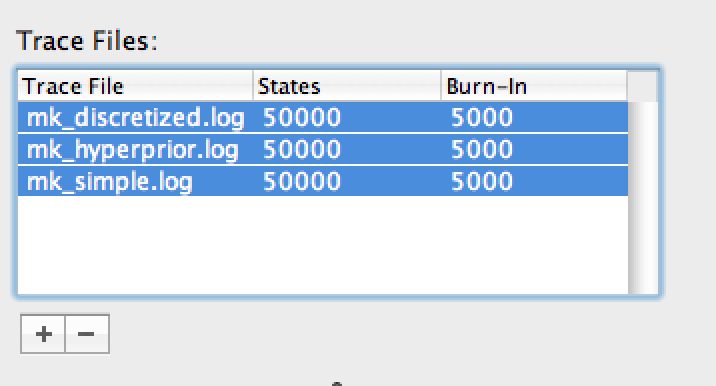
\includegraphics[width=0.5\textwidth,angle=0]{\ResourcePath figures/AddFiles}
\caption{\small Highlight all three files for model comparison.}
\end{minipage}}
\label{fig:tracer-files}
\end{figure}

Once all three trace logs are loaded and highlighted, first look at the estimated marginal likelihoods.
You will notice that the Mk model, as originally proposed by \citep{Lewis2001} is improved by allowing any state frequency heterogeneity at all. 
The discretized model and the Dirichlet model both represent improvements, but are fairly close in likelihood score to each other (Fig.~\ref{fig:tracer-llik}).
Likely, we would need to perform stepping stone model assessment to truly tell if the more complicated model is statistically justified.
This analysis is too complicated and time-consuming for this tutorial period, but you will find instructions below for performing the analysis. \par
\begin{figure}[h!]
\fbox{%
\begin{minipage}{\textwidth}\centering
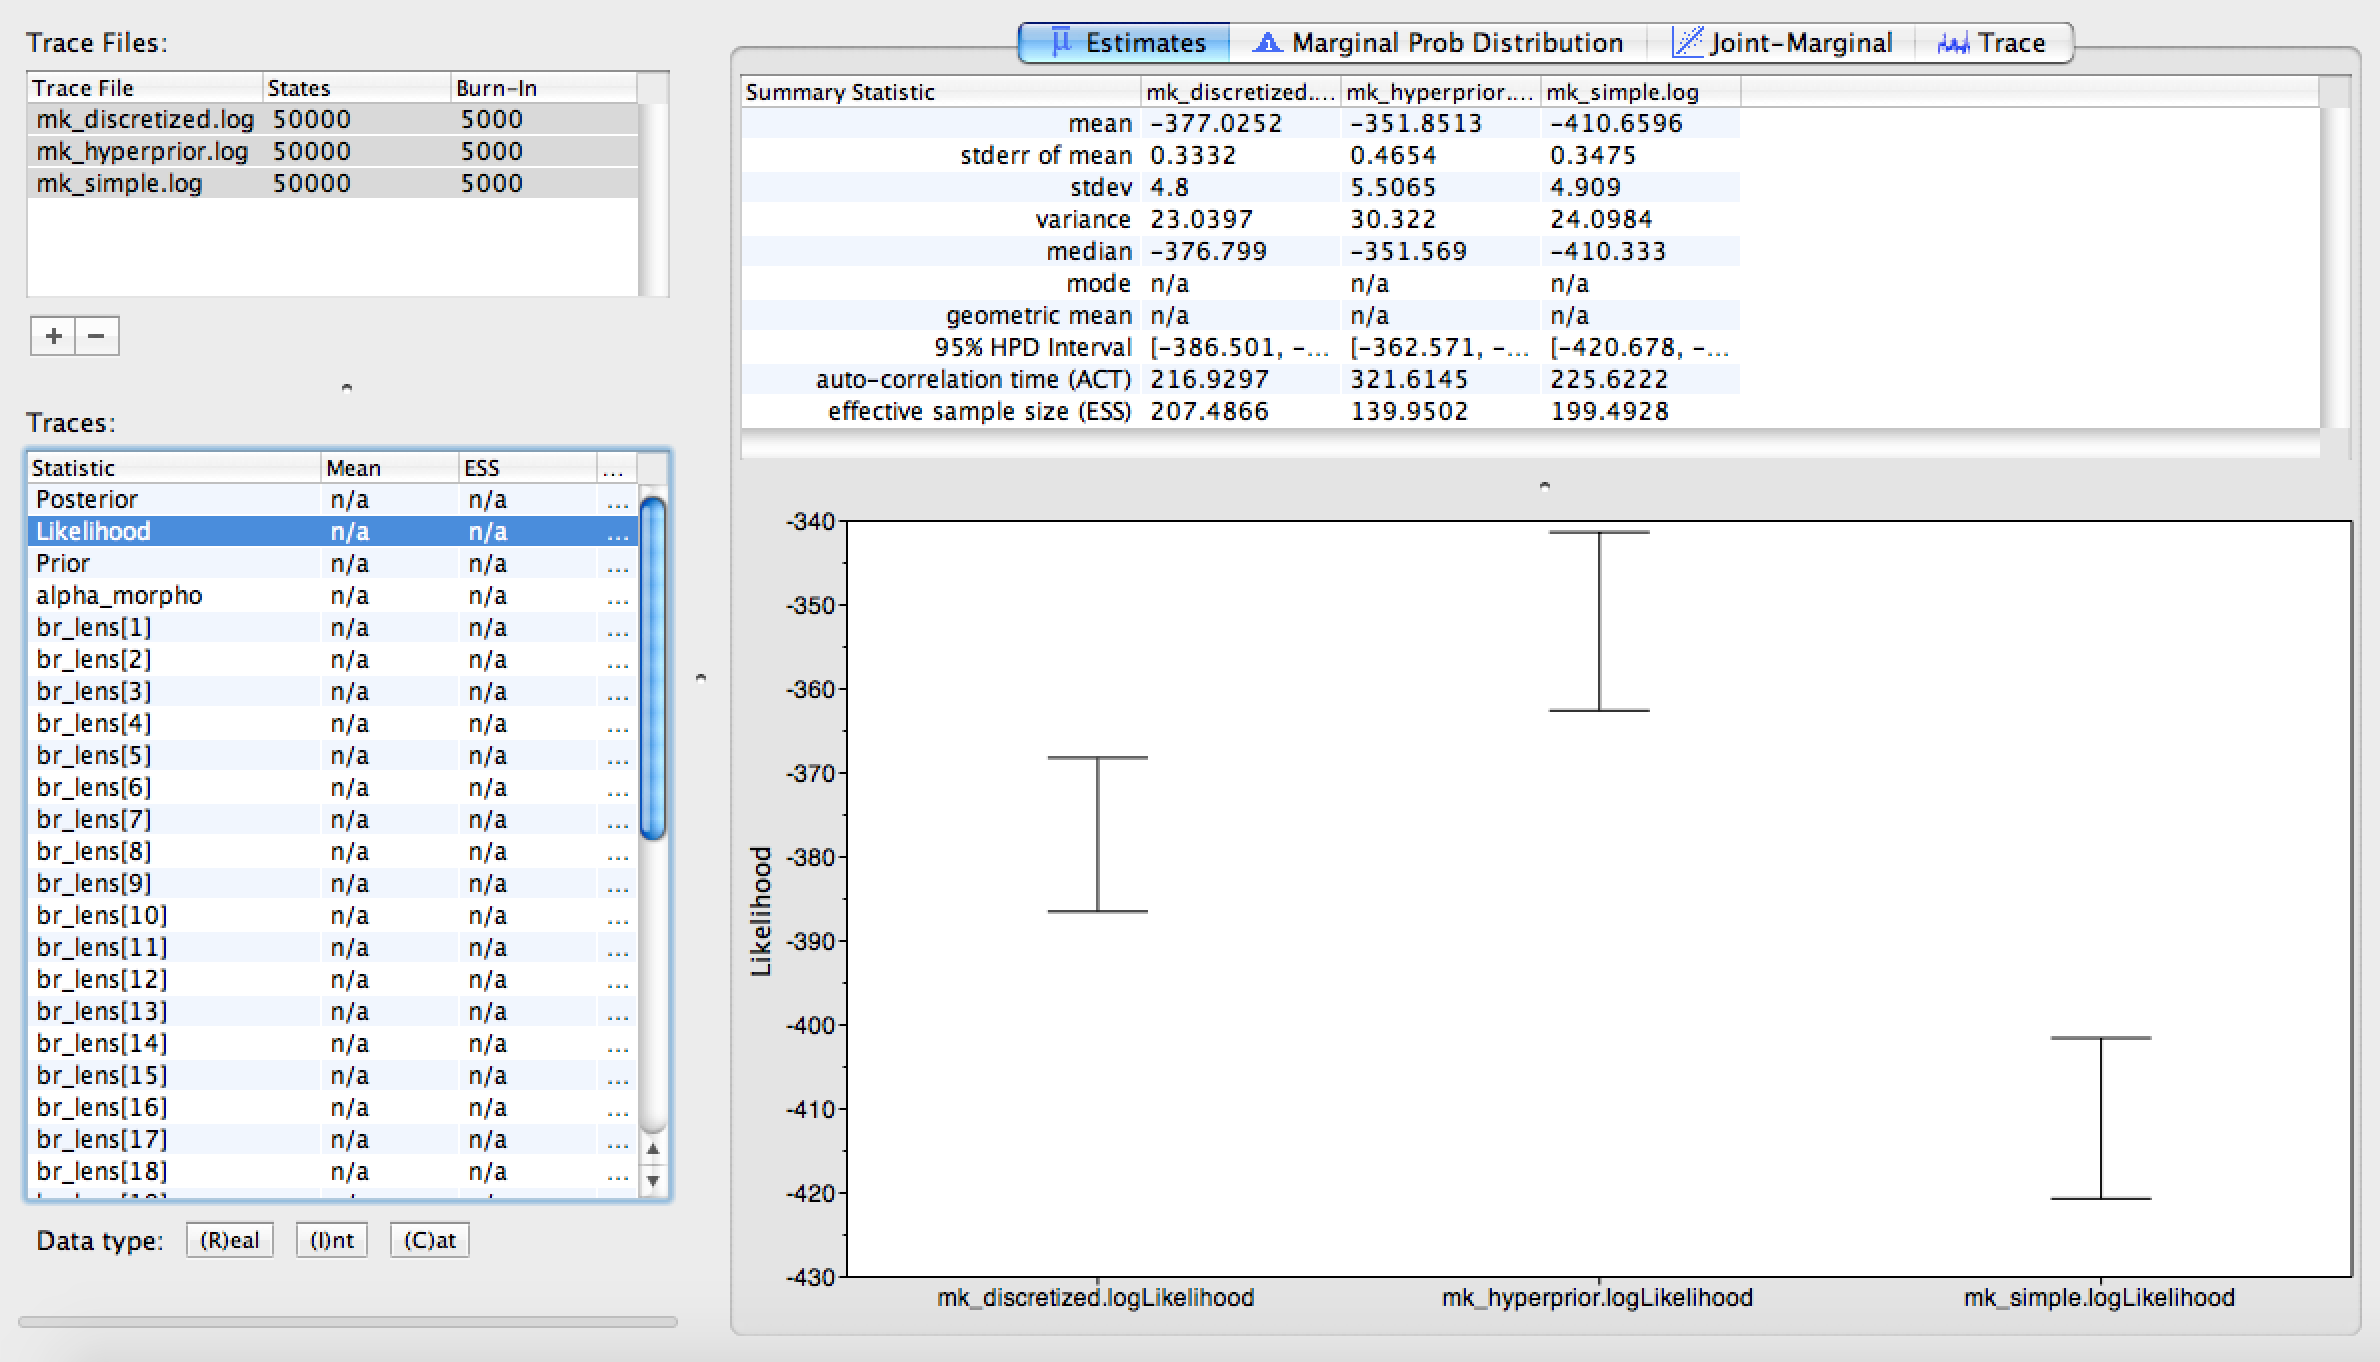
\includegraphics[width=0.75\textwidth,angle=0]{\ResourcePath figures/likelihoods}
\caption{\small Comparison of likelihood scores for all three models.}
\end{minipage}}
\label{fig:tracer-llik}
\end{figure}

Click on the `Trace' panel.
In the lower left hand corner, you will notice an option to color each trace by the file it came from.
Choose this option (you may need to expand the window slightly to see it).
Next to this option, you can also see an option to add a legend to your trace window.
The results of this coloring can be seen in Fig.~\ref{fig:coltrace}.
When the coloring is working, you will see that the Mk model mixes quite well, but that mixing becomes worse as we relax the assumption of equal state frequencies.
This is because we are greatly increasing model complexity.
Therefore, we would need to run the MCMC chains longer if we were to use these analyses in a paper. \par

\begin{figure}[h!]
\fbox{%
\begin{minipage}{\textwidth}\centering
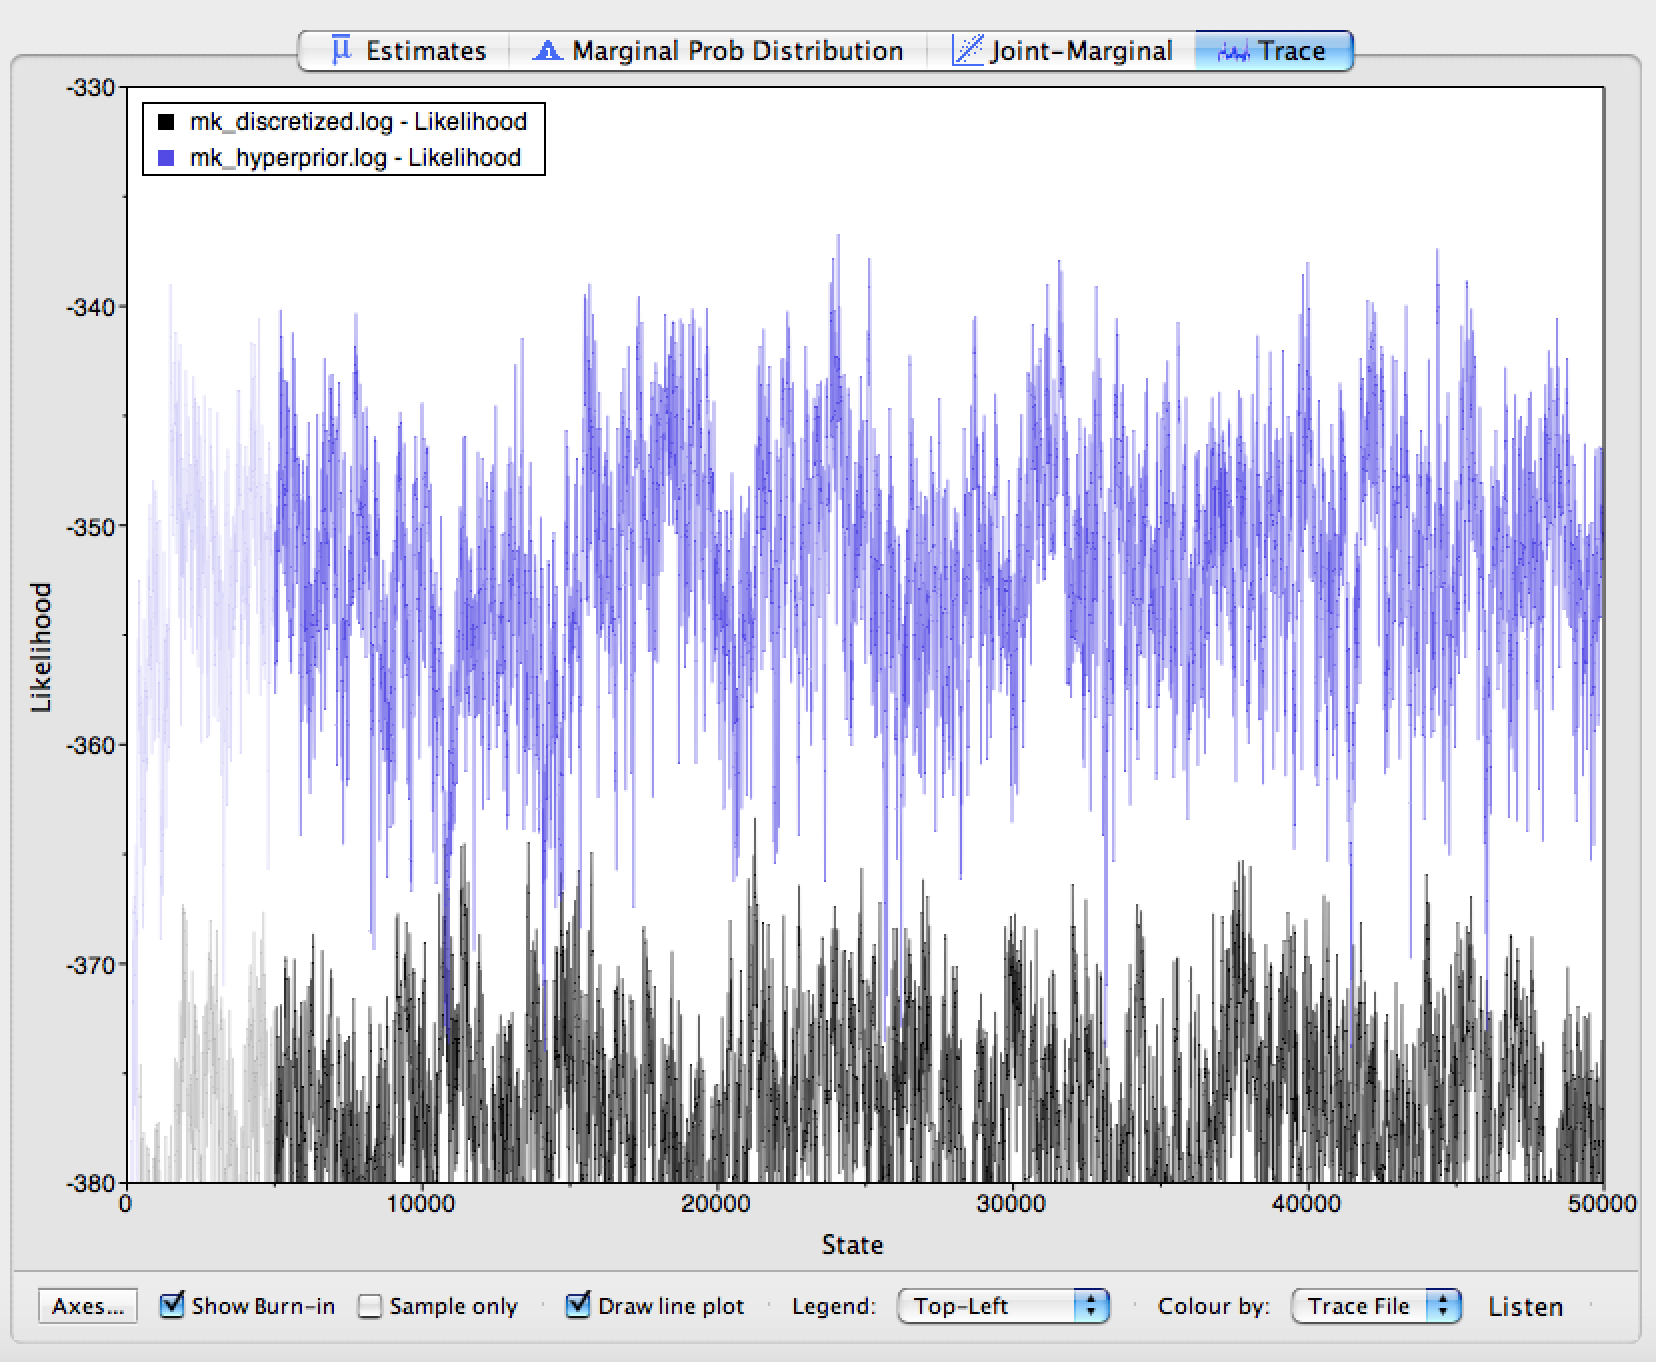
\includegraphics[width=0.6\textwidth,angle=0]{\ResourcePath figures/colortrace}
\caption{\small The Trace window. The traces are colored by which version of the Mk model they correspond to.}
\end{minipage}}
\label{fig:coltrace}
\end{figure}


We are interested in two aspects of the posterior distribution.
First, all analyses correct for the biased sampling of variable characters except for the {\tt simple} analysis.
Then, we expect the {\tt tree\_length} variable to be greater for {\tt simple} than for the remaining analyses, because our data are enriched for variation.
Figure~\ref{fig:tracer_tree_length} shows that {\tt tree\_length} is approximately 30\% greater for {\tt simple} than for {\tt mk\_simple}, which are identical except that {\tt mk\_simple} corrects for sampling bias.
To compare these densities, click the ``Marginal Prob Distribution'' tab in the upper part of the window, highlight all of the loaded Trace Files, then select {\tt tree\_length} from the list of Traces.

\begin{figure}[h!]
\fbox{%
\begin{minipage}{\textwidth}\centering
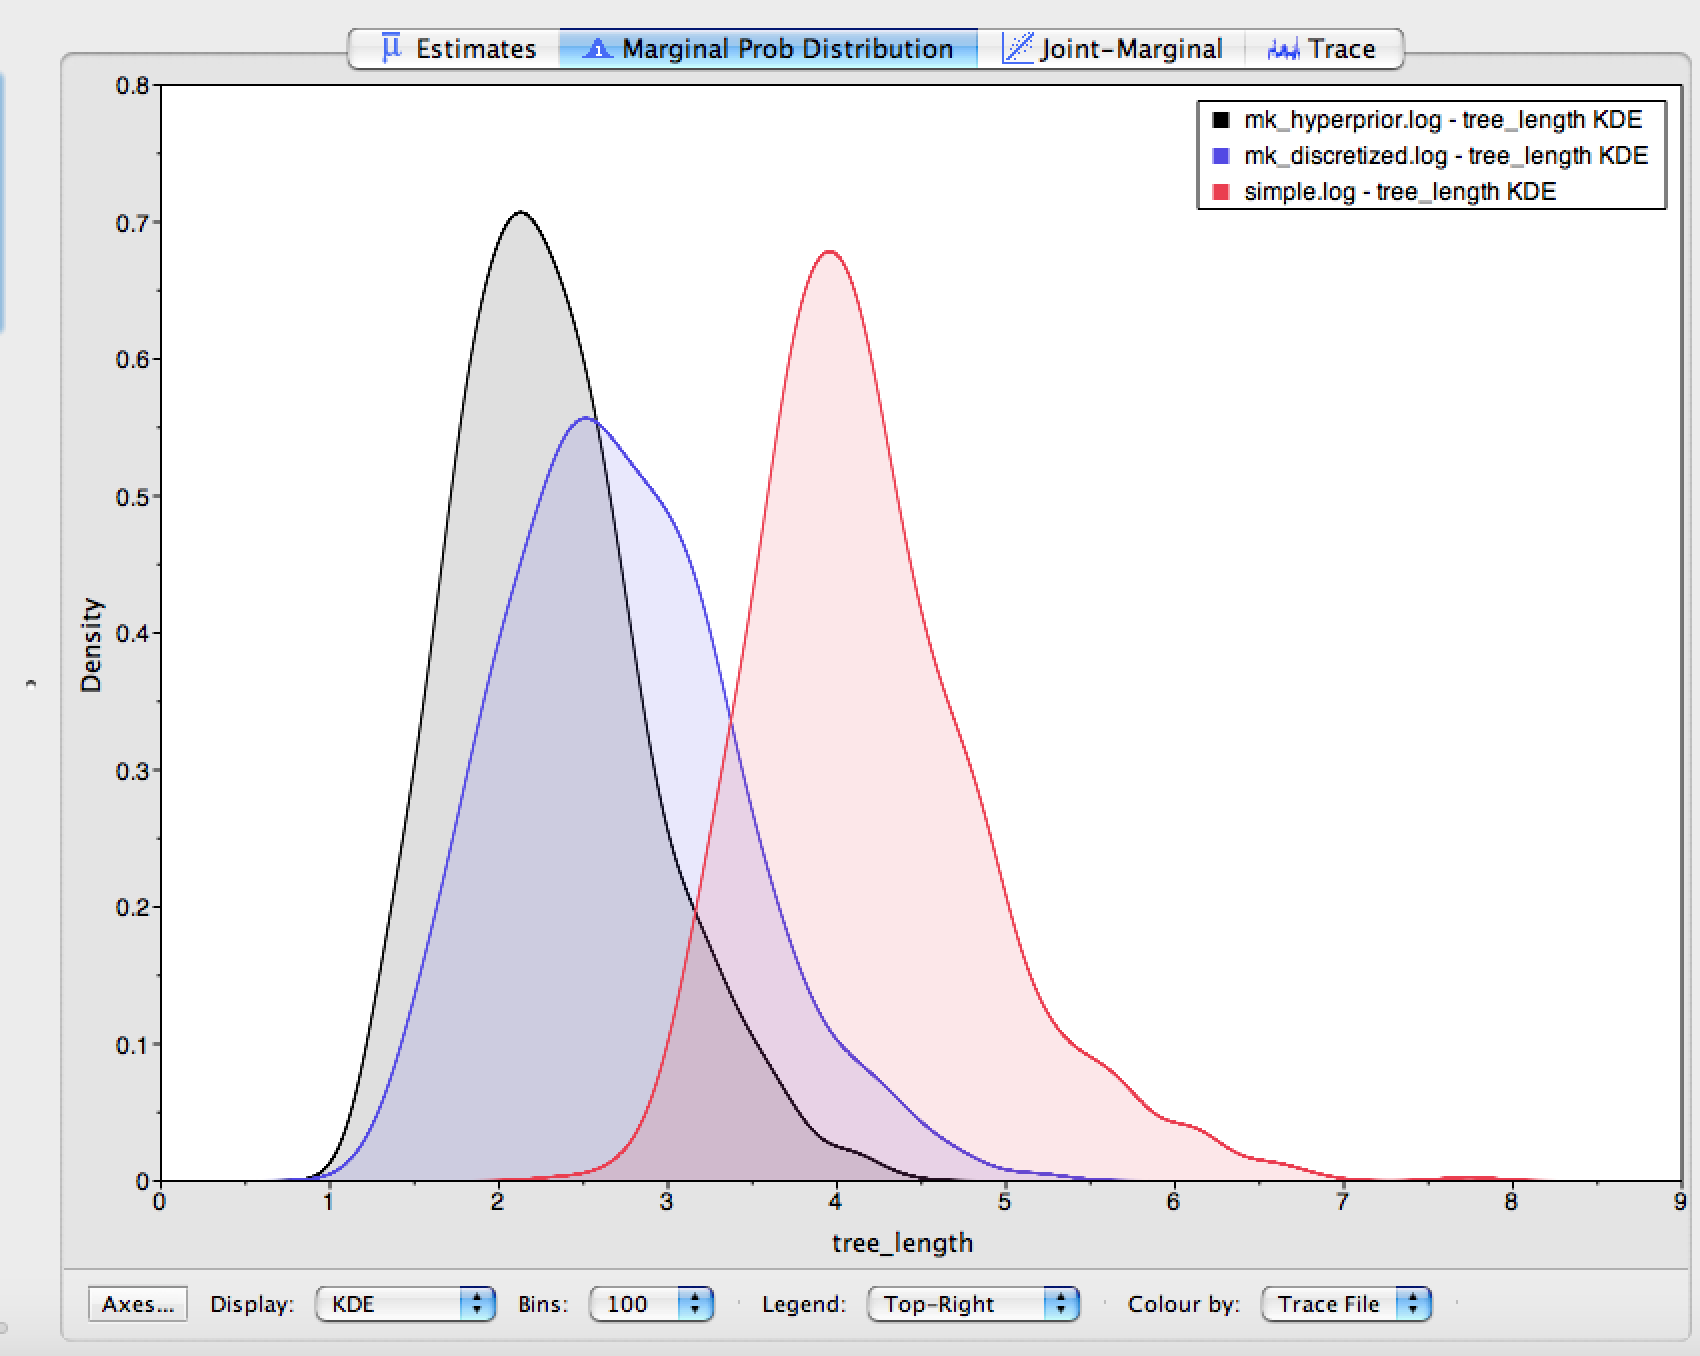
\includegraphics[width=0.9\textwidth,angle=0]{\ResourcePath figures/results/tracer_tree_length}
\caption{\small Posterior tree length estimates.}
\end{minipage}}
\label{fig:tracer_tree_length}
\end{figure}

Second, we are interested in characterizing the degree of heterogeneity estimated by the beta-discretized model.
If the data were distributed by a single morphological rate matrix, then we would expect to see very little variation among the different values in {\tt cats}, and very large values for the shape and scale parameters of the discrete-beta distribution.
For example, if {\tt alpha\_ofbeta = beta\_ofbeta = 1000}, then that would cause all discrete-beta categories to have values approaching 0.5, which approximates a symmetric Mk model.

\begin{figure}[h!]
\fbox{%
\begin{minipage}{\textwidth}\centering
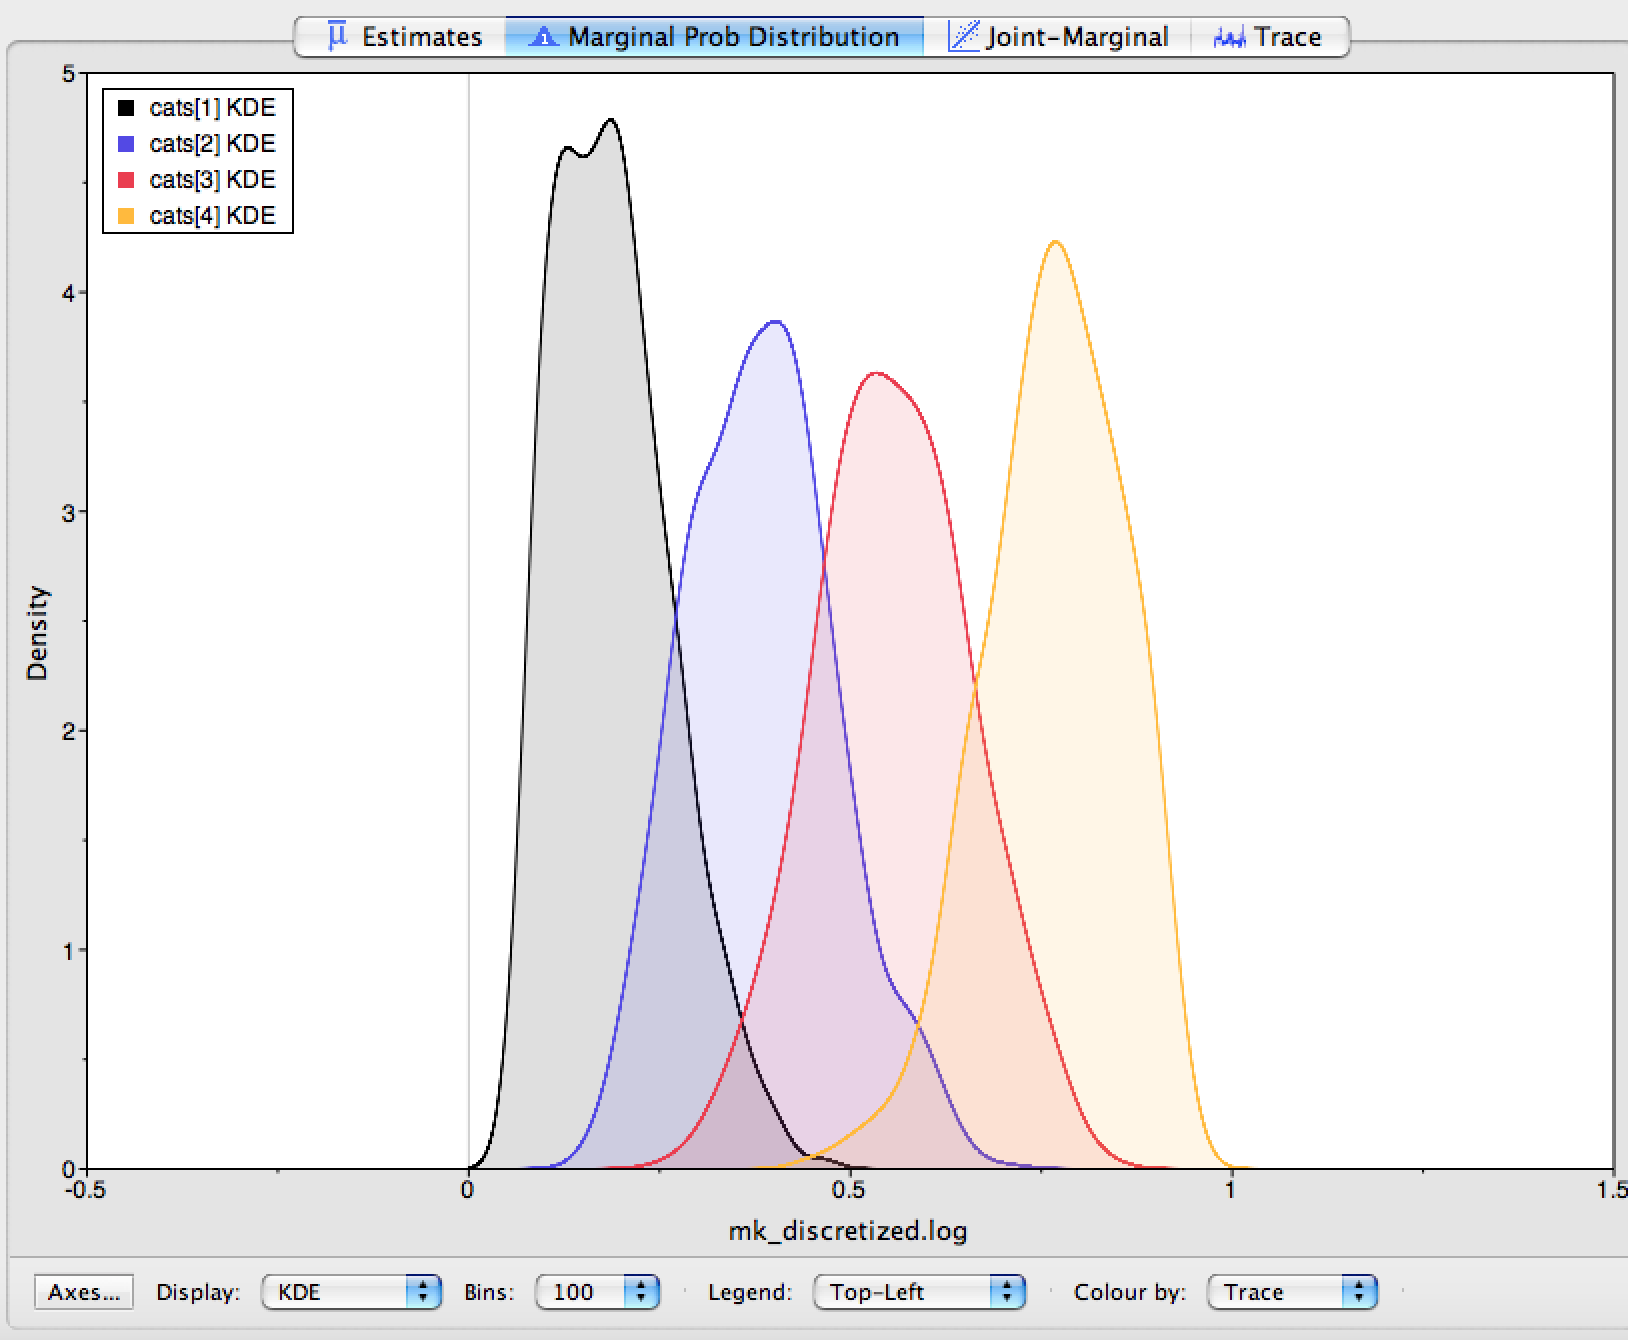
\includegraphics[width=0.9\textwidth,angle=0]{\ResourcePath figures/results/cats}
\caption{\small Posterior discretized state frequencies for the discrete-beta model.}
\end{minipage}}
\label{fig:tracer_cats}
\end{figure}

\begin{figure}[h!]
\fbox{%
\begin{minipage}{\textwidth}\centering
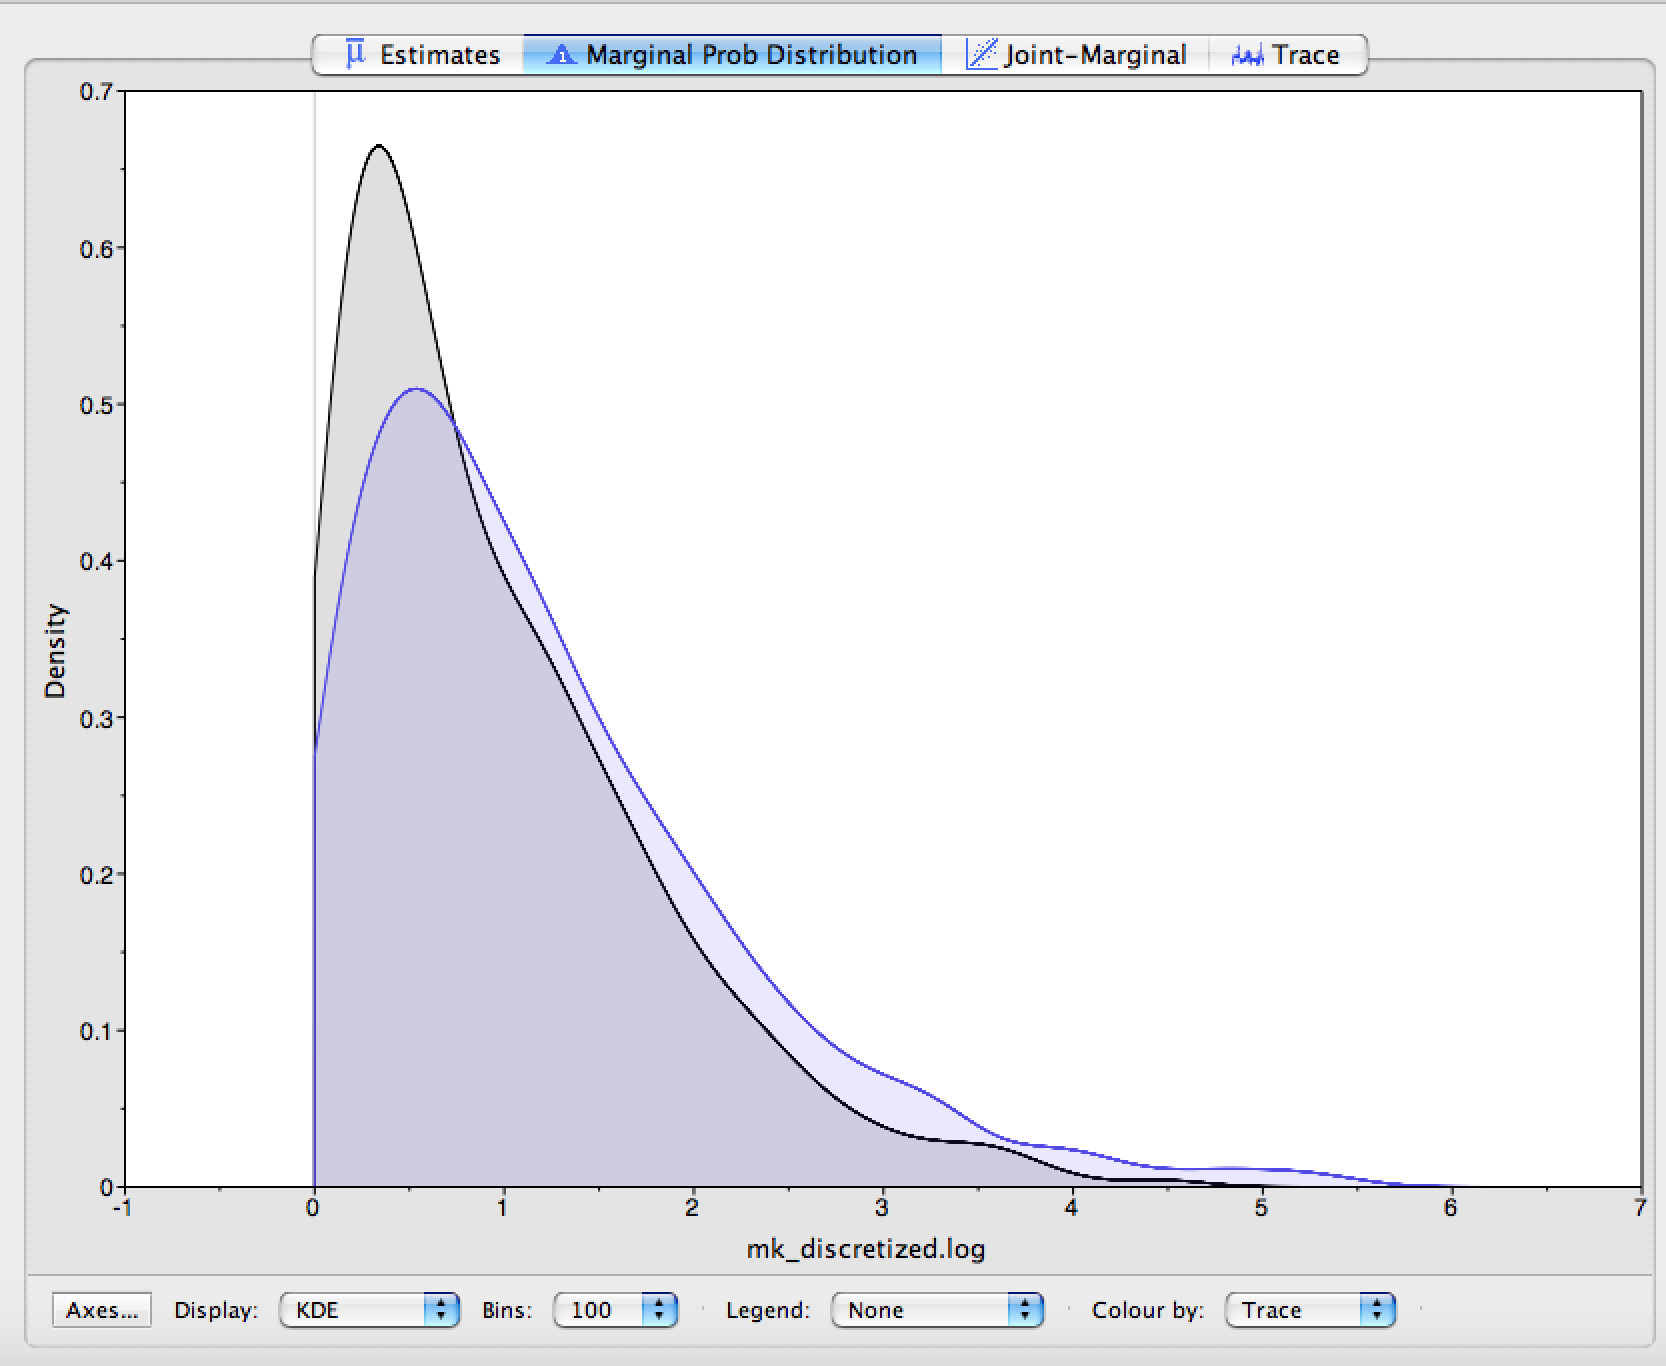
\includegraphics[width=0.9\textwidth,angle=0]{\ResourcePath figures/results/alpha_beta}
\caption{\small Posterior alpha and beta parameters for the discrete-beta model.}
\end{minipage}}
\label{fig:tracer_alpha_beta}
\end{figure}

Figure~\ref{fig:tracer_cats} shows that the four discrete-beta state frequencies do not all have the exact same value.
In addition, Figure~\ref{fig:tracer_alpha_beta} shows that the priors on the discrete-beta distribution are small enough that we expect to see variance among {\tt cat} values.
If the data contained no information regarding the distribution of {\tt cat} values, then the posterior estimates for {\tt alpha\_ofbeta} and {\tt beta\_ofbeta} would resemble the prior.

\subsection{Summarizing tree estimates}

%\begin{figure}[h!]
%\fbox{%
%\begin{minipage}{\textwidth}\centering
%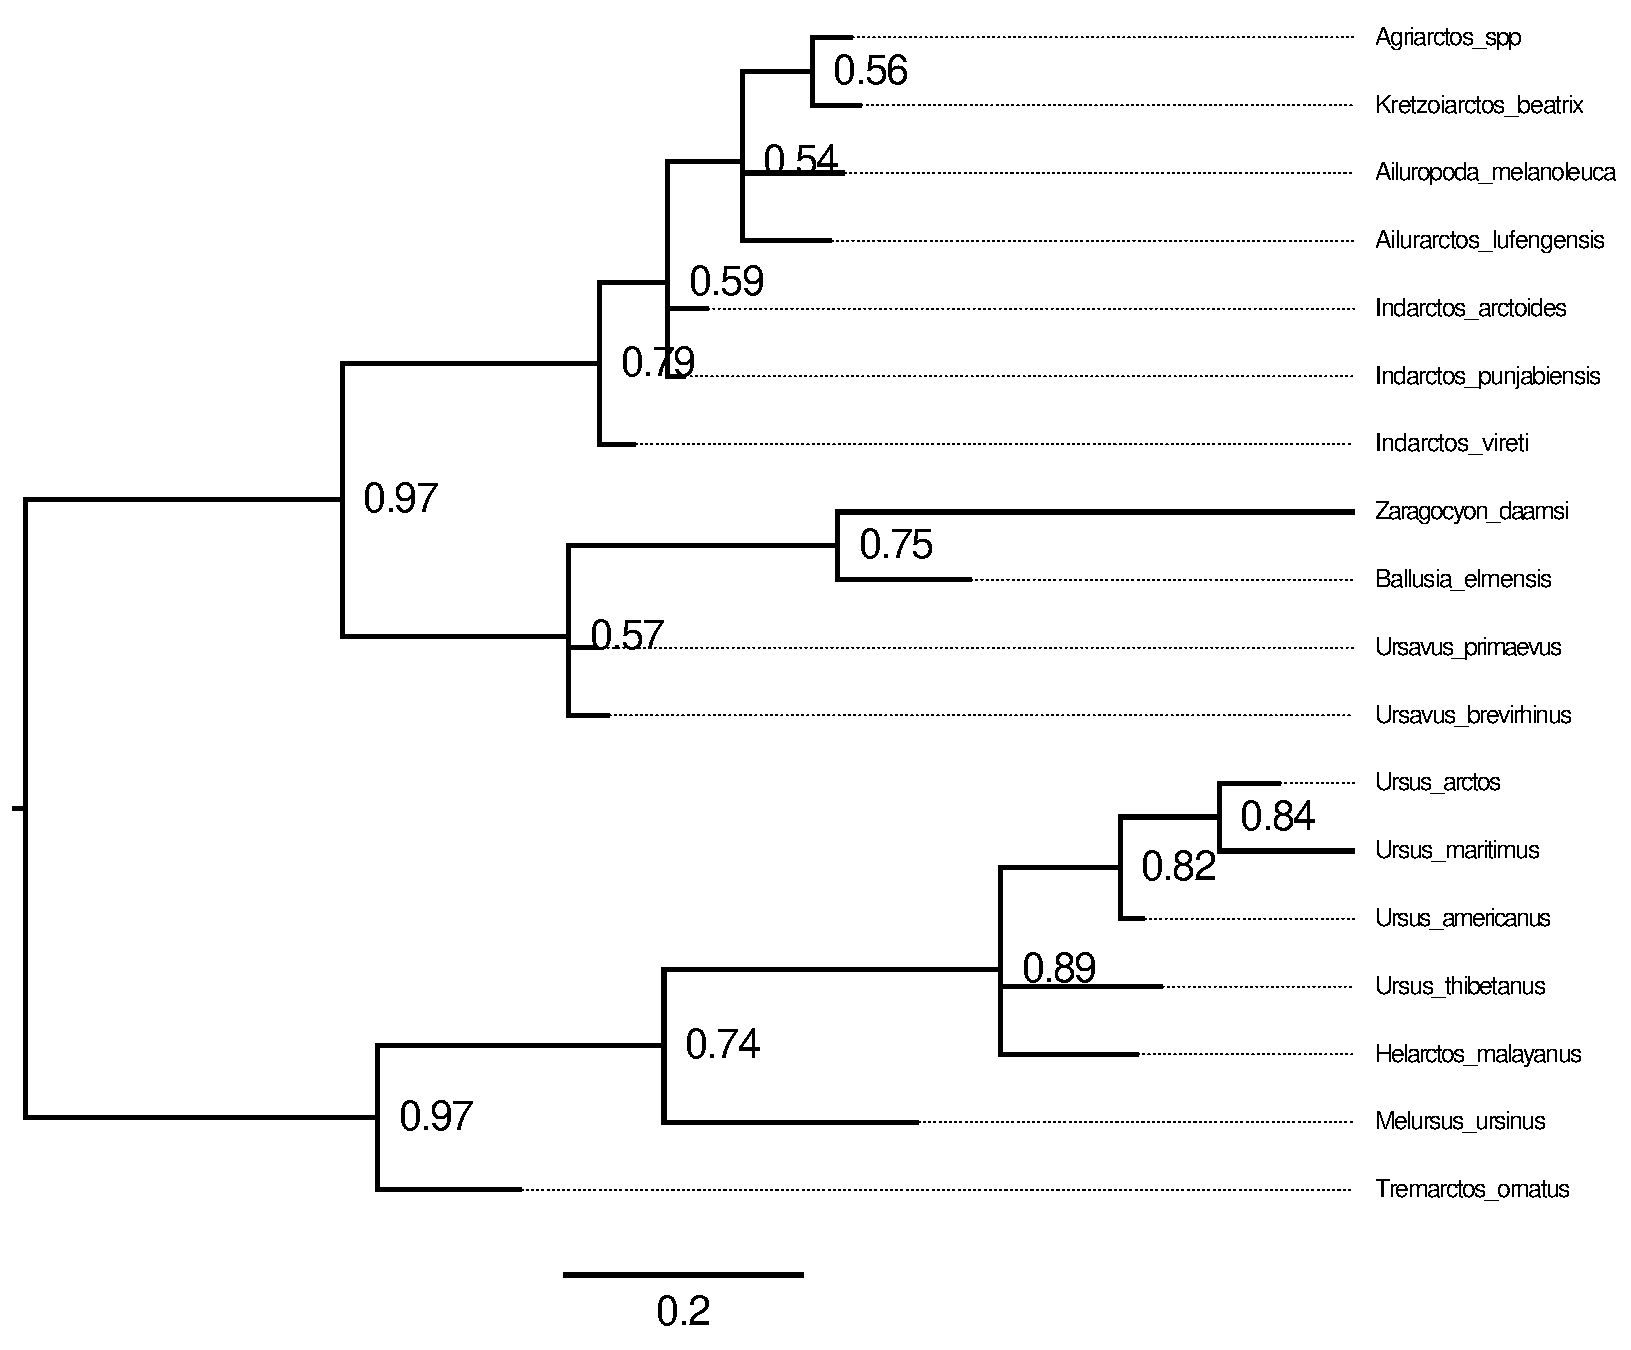
\includegraphics[width=0.6\textwidth,angle=0]{\ResourcePath figures/results/simple_majrule_tre}
%\caption{\small Majority rule consensus tree for the uniform Mk analysis.}
%\end{minipage}}
%\label{fig:simple_majrule}
%\end{figure}

The morphology trees estimated in \ref{sec:dm_simple} and \ref{sec:dm_disc} are summarized using a majority rule consensus tree (MRCT).
Clades appearing in $p>0.5$ of posterior samples are resolved in the MRCT, while poorly support clades with $p \leq 0.5$ are shown as unresolved polytomies.
%Poor support for clades is typically caused by either having too little  conflicting phylogenetic information.
Poor phylogenetic resolution might be caused by having too few phylogenetically informative characters, or it might be due to conflicting signals for certain species relationships.
Because phylogenetic information is generated through model choice, let's compare our topological estimates across models.

\begin{figure}[h!]
\fbox{%
\begin{minipage}{\textwidth}\centering
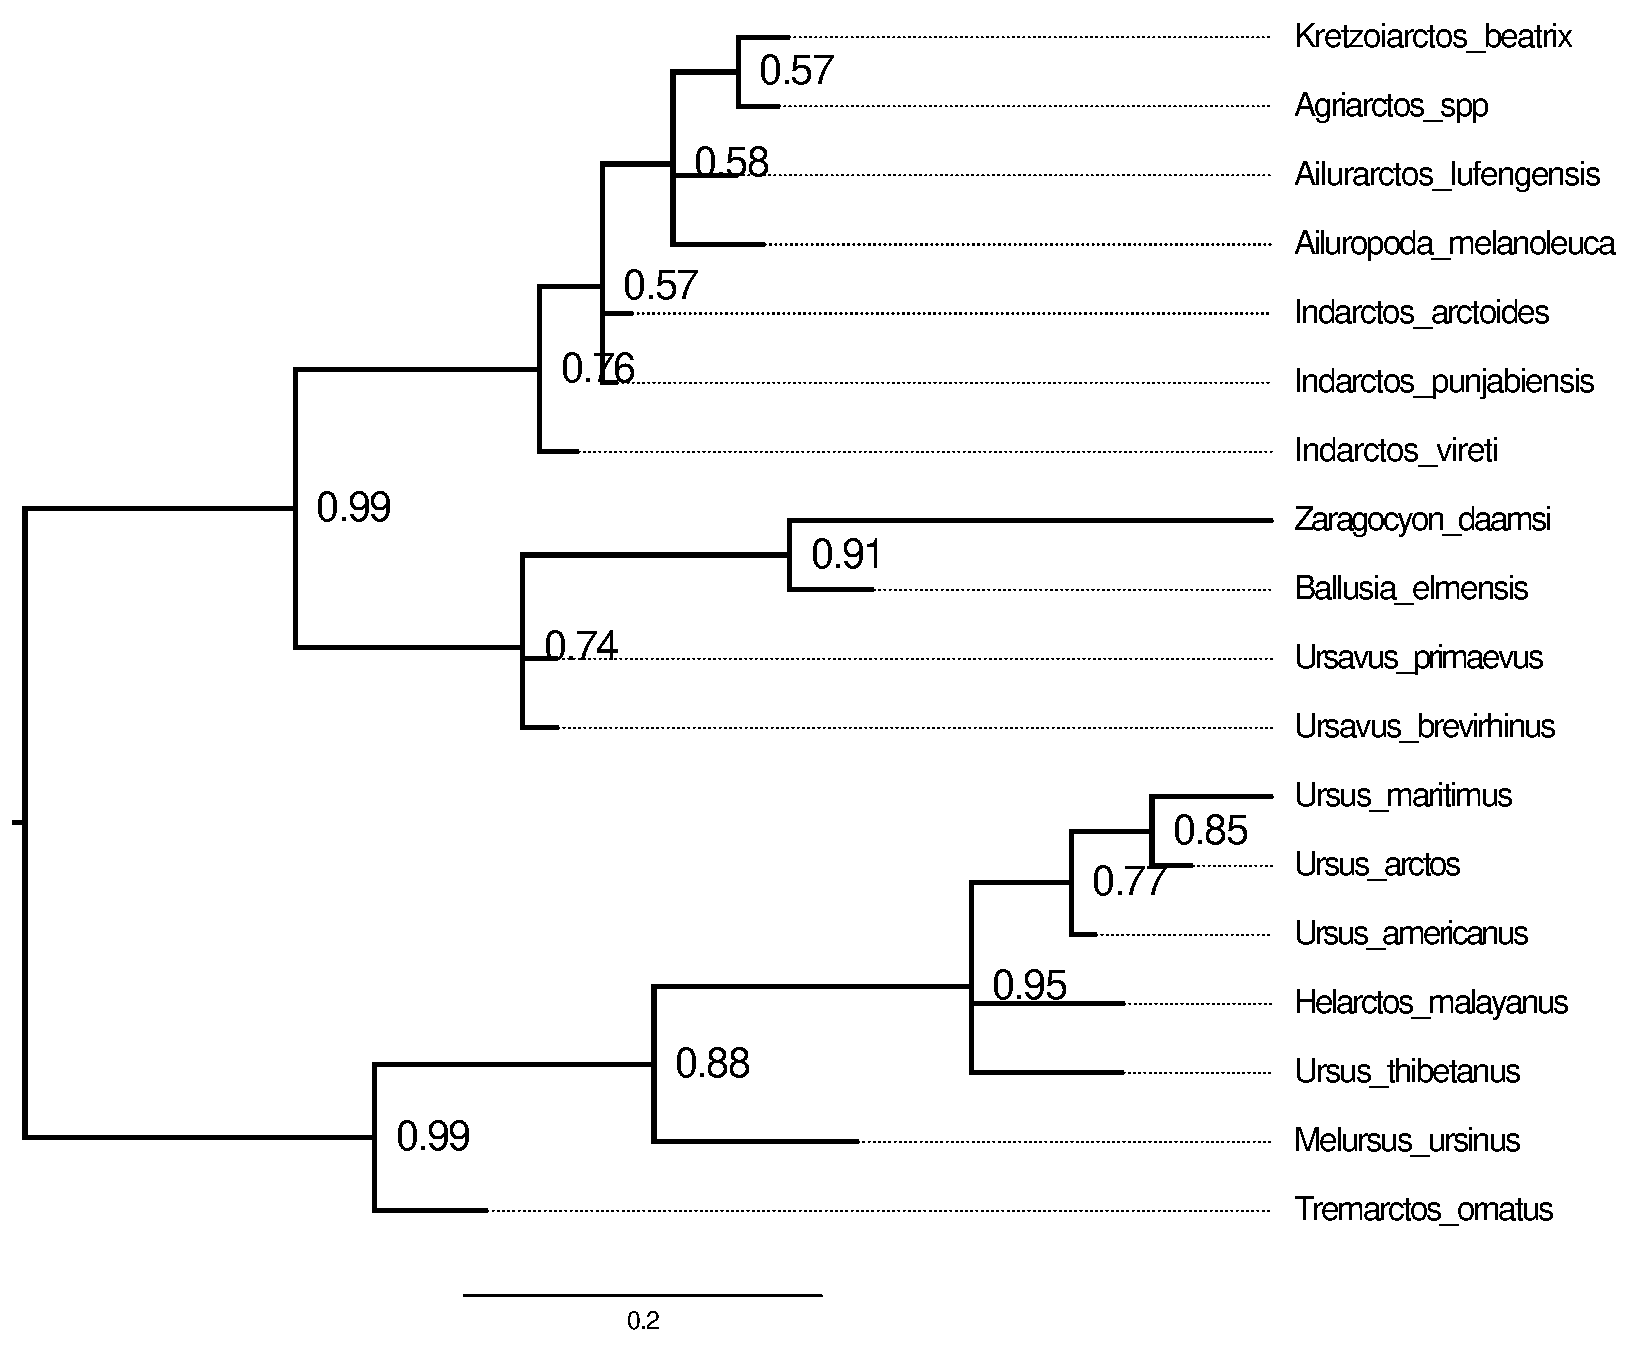
\includegraphics[width=0.6\textwidth,angle=0]{\ResourcePath figures/results/mk_discretized_majrule_tre}
\caption{\small Majority rule consensus tree for the beta-discretized Mkv analysis.}
\end{minipage}}
\label{fig:mk_discretized_majrule}
\end{figure}

The MRCTs for the simple model with and without the +v correction are very similar to that for the discretized-beta model (Fig.~\ref{fig:mk_discretized_majrule}).
Note that the scale bars for branch lengths differ greatly, indicating that tree length estimates are inflated without the +v correction, just as we saw when comparing the posterior tree length densities.
In general, it is important to assess whether your results are sensitive to model assumptions, such as the degree of model complexity, and any mechanistic assumptions that motivate the model's design.
In this case, our tree estimate appears to be robust to model complexity.

%\subsection{Ancestral state estimation} \label{sec:anc_states}
%
%Discrete morphological models are not only useful for tree estimation, as was done in Section \ref{sec:dm_overview}, but also for ancestral state estimation.
%The central problem in statistical phylogenetics concerns {\it marginalizing} over all unobserved character histories that evolved along the branches of a given phylogenetic tree according to some model, $M$, under some parameters, $\theta$.
%This marginalization yields the probability of observing the tip states, $X_\text{tip}$, given the model and its parameters, $P( X_\text{tip} | \theta, M ) = \sum_{X_\text{internal}} P( X_\text{internal}, X_\text{tip} \mid \theta, M )$.
%One might also wish to find the probability distribution of ancestral state configurations that are consistent with the tip state distribution, $P( X_\text{internal} \mid X_\text{tip}, \theta, M )$, and to sample ancestral states from that distribution.
%This procedure is known as {\it ancestral state estimation}.
%
%There are several strategies for ancestral state estimation, each with their own advantages and disadvantages.
%One can compute the {\it exact probability} of any given ancestral node having an ancestral state value; or one can {\it sample} states from that distribution in proportion to the exact probability.
%One can produce {\it marginal} ancestral state estimates that report how often any given node is in a state without the context of the ancestral states of the remaining nodes; or one can produce {\it joint} ancestral state estimates that report the probability of particular combinations of sequences of evolutionary histories, running from the root to the tips of the phylogeny.
%
%While it is straightforward to produce exact probabilities for marginal histories, sampling is generally required to produce joint histories.
%Exact marginal approaches are fast, accurate, and compact, while joint sampling approaches require more samples to achieve accuracy comparable to marginal estimates, along with large files to store those samples.
%While one can obtain marginal estimates from joint estimates, one cannot obtain joint estimates from marginal estimates.
%
%This tutorial uses a joint sampling strategy because they yield the most complete representation of possible evolutionary scenarios.
%
%\subsection{Ancestral state monitors}
%
%The completed exercises from Section \ref{sec:dm_overview} made use of a monitor names {\tt mnJointConditionalAncestralState}, which was created with the command
%
%{\tt \begin{snugshade*}
%\begin{lstlisting}
%monitors[mni++] = mnJointConditionalAncestralState(tree=phylogeny,
%                                                   ctmc=phyMorpho,
%                                                   filename="output/simple.states.txt",
%                                                   type="Standard",
%                                                   printgen=10,
%                                                   withTips=false)
%\end{lstlisting}
%\end{snugshade*}}
%
%The core arguments this monitor needs are a tree object ({\tt tree=phylogeny}), the phylogenetic model ({\tt ctmc=phyMorpho}), an output filename ({\tt filename="output/simple.states.txt"}), the data type for the characters ({\tt type="Standard"}), and the sampling frequency ({\tt printgen=10}).
%The final argument, {\tt withTips=false}, indicates that we do not wish to record the starting state for each branch, since it will always be identical to the ending state of the parental branch (but this is not necessarily so for models with cladogenesis).
%
%The monitor will produce a joint sample of ancestral states (conditional on the tip states) every 10 iterations, storing the samples to the file {\tt "output/simple.states.txt"}.
%Viewing the states file, we see
%
%{\tt \begin{snugshade*}
%\begin{lstlisting}
%|*Iteration	end_1	end_2	end_3	end_4
%|*0	?,0,?,?,?,?,?,?,?,?,?,?,?,?,?,?,0,0,0, ...
%|*10	?,0,?,?,?,?,?,?,?,?,?,?,?,?,?,?,0,0,0, ...
%|*20	?,0,?,?,?,?,?,?,?,?,?,?,?,?,?,?,0,0,0, ...
%|*30	?,0,?,?,?,?,?,?,?,?,?,?,?,?,?,?,0,0,0, ...
%|*40	?,0,?,?,?,?,?,?,?,?,?,?,?,?,?,?,0,0,0, ...
%|*50	?,0,?,?,?,?,?,?,?,?,?,?,?,?,?,?,0,0,0, ...
%|*...
%\end{lstlisting}
%\end{snugshade*}}
%
%The first column is the MCMC iteration, and the remaining columns represent the states sampled at end of the branch for an indexed node.
%When the phylogeny is a random variable, the index is used to map an ancestral state estimate to the node in any given tree sample from the analysis.
%The vector of comma-delimited ancestral state estimates is reported for each column value.
%In the example above, we see that the node indexed 1 (a tip node) always produces the observed character matrix [ future versions will sample ambiguous tip states, e.g. {\tt ?} ].
%The first $1 \ldots N$ index values are assigned to tip nodes in a tree with $N$ tips.
%We observe the uncertainty in our ancestral state estimates by viewing the final column
%
%{\tt \begin{snugshade*}
%\begin{lstlisting}
%[ column headers are far to the left ]
%|*... 1,0,1,0,1,0,1,1,0,0,0,1,1,1
%|*... 1,1,1,1,1,0,0,1,0,0,1,1,1,0
%|*... 1,1,1,0,0,0,0,0,0,0,0,0,1,0
%|*... 1,1,0,1,1,0,1,0,0,1,0,0,1,0
%|*... 1,1,0,1,1,0,1,0,1,0,0,0,1,0
%|*... 1,1,0,1,1,0,1,0,1,1,0,0,1,0
%|*...
%\end{lstlisting}
%\end{snugshade*}}
%
%\subsection{Ancestral state figures}
%
%Now that we have our posterior distribution of ancestral states and of phylogenetic trees, we want to summarize those results into something simpler.
%This section will aim to produce a pdf containing figures for the ancestral state estimates mapped onto a consensus tree for all 62 characters.
%
%\subsection{Output processing}
%
%To accomplish this, we will rely on a combination of \RevBayes, {\tt R}, and {\tt bash} scripts.
%The contents of the following scripts demonstrate how one might integrate \RevBayes into a pipeline to process output using a variety of tools.
%Precomputed results are found in {\tt example\_output}.
%[ Unfortunately, this exact pipeline probably does not work for Windows users at this time. ]
%
%To generate the figure {\tt output/mk\_simple.char\_1\_to\_5.pdf} containing ancestral state estimates for characters 1 through 5, use the following command
%
%{\tt \begin{snugshade*}
%\begin{lstlisting}
%./scripts/make_anc_trees.sh output/mk_simple 1 5
%\end{lstlisting}
%\end{snugshade*}}
%
%This shell script first generates ancestral state trees using the analysis files prefixed with {\tt "output/mk\_simple"} for characters {\tt 1} through {\tt 5} by piping those variables into the \RevBayes script {\tt scripts/make\_anc\_states.Rev}.
%The {\tt make\_anc\_states.Rev} script produces a series of tree files annotated with the ancestral state estimates and probabilities named e.g. {\tt mk\_simple.char\_1.ase.tre}.
%Next, the shell script calls {\tt Rscript} to execute {\tt scripts/plot\_anc\_state.R} using the tree filenames as arguments.
%The {\tt plot\_anc\_states.R} file produces a tree figure for each file using the {\tt R} package, {\tt RevGadgets}.
%Finally, the shell script combines the resulting figures into a single concatenated pdf using the tool {\tt gs}.
%
%
%
%{\tt \begin{snugshade*}
%\begin{lstlisting}
%./scripts/make_anc_trees.sh output/mk_simple 1 5
%\end{lstlisting}
%\end{snugshade*}}
%
%
%
%
%\subsection{Results}
%
%\begin{figure}[h!]
%\fbox{%
%\begin{minipage}{\textwidth}\centering
%\includegraphics[width=0.92\textwidth,angle=0]{\ResourcePath figures/results/mk_simple_char_36_ase}
%\caption{\small Ancestral state estimates assuming the uniform Mk model for character 36.}
%\end{minipage}}
%\label{fig:mk_simple_ase}
%\end{figure}
%
%Knowing what we do about the various models, how might we expect the ancestral state estimates to differ?
%For one, the {\tt simple} model does not condition on ascertainment bias towards variable characters.
%This leads to overestimated branch lengths when compared to the {\tt mk\_simple} model.
%
%\begin{figure}[h!]
%\fbox{%
%\begin{minipage}{\textwidth}\centering
%\includegraphics[width=0.92\textwidth,angle=0]{\ResourcePath figures/results/mk_discretized_char_36_ase}
%\caption{\small Ancestral state estimates assuming the beta-discretized Mkv model for character 36.}
%\end{minipage}}
%\label{fig:mk_discretized_ase}
%\end{figure}
%
%We might expect that {\tt mk\_simple}, because it forces all characters to evolve under a single symmetric model of evolution, would have more ambiguity in ancestral state estimates.
%In contrast {\tt mk\_discretized} allows characters to evolve with different tendencies towards 0- or 1-valued states, which might increase the certainty in ancestral state estimates.
%
%Many ancestral state estimates are fairly insensitive to model choice, particularly for characters that underwent only a single transition.
%Characters that underwent a reversion are more sensitive.
%Character 36, for example:
%Figure \ref{fig:mk_simple_ase} shows that the uniform Mkv model has a weak preference for the two immediate ancestral nodes for {\it Melursus urisinus} and {\it Tremarctos ornatus} to be in the absent state ($p < 0.55$).
%Figure \ref{fig:mk_simple_ase}) shows that the discretized-beta model provides stronger and contradictory support for the present state ($0.65 \leq p \leq 0.70$).



\bibliographystyle{sysbio}
\bibliography{\GlobalResourcePath refs}



\part{Phylogenetic Comparative Method}
\chapter{Phylogenetic Comparative Analyses: Continuous Trait Evolution}
\def \ResourcePath {RB_PhyloComparative_Tutorial/}
\include{RB_PhyloComparative_Tutorial/RB_PhyloComparative_Tutorial_content}



\end{document}
